% !TEX program = lualatex
\documentclass[UTF8]{ctexbook}
\usepackage[a4paper,margin=2.5cm]{geometry}\usepackage{amsmath,amssymb,amsthm}
\usepackage{graphicx}
\usepackage{hyperref}
\usepackage{booktabs}
\usepackage{array}
\newcolumntype{C}[1]{>{\centering\arraybackslash}m{#1}}
\usepackage{tikz}
\usepackage{tikz-cd}
\usepackage{multicol}

\usepackage{wrapfig}
\usepackage{float}
\usepackage{subcaption}

\usepackage{needspace}

\usepackage{xcolor}

% 定义纯黑白灰颜色
\definecolor{bg}{HTML}{FFFFFF}       % 白色背景
\definecolor{highlight}{HTML}{000000} % 纯黑 (显色数字)
\definecolor{dim}{HTML}{A3A3A3}      % 浅灰 (暗数字，调白了)
\definecolor{labelcolor}{HTML}{000000}

\newtheorem{definition}{定义}[section]
\newtheorem{theorem}{定理}[section]
\newtheorem{example}{例}[section]

\usetikzlibrary{arrows.meta,positioning,calc}
\newcommand{\R}{\mathbb{R}}
\raggedbottom

\begin{document}

\tableofcontents



\chapter{几何学}



描述世界的第一步就是描述物体的位置，我们最熟知的方法就是建立坐标系，从一维数轴，到二维的平面直角坐标系，到三维的空间直角坐标系，我们描述位置的难度也在不断增加，每增加一个维度，确定一个点的参数就增加一个。

在一维中，我们研究的对象只有点；二维则包括点和线；三维则包括点，线和面。点动成线，所以只要将点的两个坐标都换成关于某一参数的函数，那么所有这么确定的点组成的集合就是线，三维的线也同理。
\[
\Gamma=\left\{(x,y,z)\in\mathbb{R}^3\ \middle|\
\begin{aligned}
x&=x(t),\\
y&=y(t),\\
z&=z(t),\quad t\in I
\end{aligned}
\right\}
\]
而描述三维空间中的平面，只需要减少集合的一个约束，比如我们舍去关于$y$坐标的约束，那么这个点集描述的其实就是一个面，所有的点都在这个面内，不难看出维数和约束存在某种关系，只有当维数和约束的个数达到统一的时候才能描写具体的一个点。我们管这样的约束叫做自由度，这也就是说三维空间有三个自由度，而二维空间有两个自由度，因而只需要两个约束就可以描述一个平面。
\[
\Gamma=\left\{(x,y,z)\in\mathbb{R}^3\ \middle|\
\begin{aligned}
x&=x(t),\\
z&=z(t),\quad t\in I
\end{aligned}
\right\}
\]

这样我们就有足够的能力描述一个空间对象了，但是我们又该如何描述它的性质呢？就像二维的线我们使用切线描述，三维则更复杂，不仅曲线有切线，曲面还会有切平面，此外还有法平面这样的东西，我们又该如何描述？

描述一个几何体，首先还是要描述它的几何性质——长度，面积和体积。无论几维空间，距离都可以根据勾股定理由三个坐标差的平方和再开根得到，面积就更加复杂，一般需要使用在知道边长后结合正余弦定理才可以得到，体积就更别说了，即使是高中的学习也为曾涉及太多。

为了建立一个统一的数学工具，数学家发明了向量，它是一个有方向的量，从起始点指向终点，在物理学中我们称之为位矢，可以很好的描述物体间的相对位置，所以讲解解析几何就要先从向量说起。

\newpage

\section{向量运算}

解析几何的基础就是点，线，面可以在三维直角坐标系中定量表示，我们接下来的讨论都基于在三维坐标系中的向量
\[
\mathbf{a}=(a_1,a_2,a_3),\quad \mathbf{b}=(b_1,b_2,b_3),\quad \mathbf{c}=(c_1,c_2,c_3).
\]

\subsection{数量积（点积）}
\label{dotp}

我们在许多的物理问题中，都会遇到一个矢量在另一个矢量上投影的积这样的运算，这主要是为了描述只有共线的成分可以为某个量做贡献的情况，比如功之类的。在一维坐标系中，就只是两个向量长度乘积；在二维坐标系中，可以表示为$\mathbf{a}\cdot\mathbf{b}=|\mathbf{a}|\,|\mathbf{b}|\cos\theta$，我们数学定理在任意维度上是对称的，所以我们可以将该式推广到任意维度，也就是说数量积的定义是
\[
\mathbf{a}\cdot\mathbf{b}=|\mathbf{a}|\,|\mathbf{b}|\cos\theta,
\]
其中 $\theta$ 为 $\mathbf{a}$ 与 $\mathbf{b}$ 的夹角（$0\le \theta \le \pi$）。所以数量积也可以帮助我们求解向量的夹角。

数量积刻画一个向量在另一个向量方向上的投影程度。
在直角坐标系中，$\mathbf{a}$ 与 $\mathbf{b}$ 的点积可以被表示为坐标积之和，在三维直角坐标系中就是：
\[
\mathbf{a}\cdot\mathbf{b}=a_1b_1+a_2b_2+a_3b_3.
\]
由此可得
\[
|\mathbf{a}|=\sqrt{\mathbf{a}\cdot\mathbf{a}}=\sqrt{a_1^2+a_2^2+a_3^2},
\quad
\cos\theta=\frac{\mathbf{a}\cdot\mathbf{b}}{|\mathbf{a}|\,|\mathbf{b}|}.
\]
从这个公式我们不仅可以求得一个向量在另一个向量方向上的投影程度，更可以求解任意两个向量的角度。因此在接下来的学习中，我们可以通过运算方向向量和法向量的夹角来表征线和面的关系。


\subsection{向量积（叉积）}

在物理世界中向量积也极经常被使用，
两个向量的向量积定义为
\[
\mathbf{a}\times\mathbf{b}
=|\mathbf{a}|\,|\mathbf{b}|\sin\theta\,\mathbf{n},
\]
其中 $\mathbf{n}$ 是与 $\mathbf{a},\mathbf{b}$ 都垂直的单位法向量，方向由右手定则确定。显然它在向量空间的运算意义就是产生一个新的基（或者说新的维度，在线性代数章节会介绍），而我们使用它更多是为了得到法向量。

此外，从表达式不难看出，它很像正弦定理推导出的面积公式，所以向量积具有的\textbf{几何意义}是$|\mathbf{a}\times\mathbf{b}|$ 等于以 $\mathbf{a},\mathbf{b}$ 为邻边的平行四边形面积，所以许多和面积有关的物理定律，比如开普勒第二定律，都最终被表示为向量积的运算；
此外，若 $\mathbf{a}\times\mathbf{b}=\mathbf{0}$，则 $\mathbf{a},\mathbf{b}$ 共线（或有零向量）。




在三维直角坐标系中，其运算可以写作：
\[
\mathbf{a}\times\mathbf{b}
=\begin{vmatrix}
\mathbf{i} & \mathbf{j} & \mathbf{k}\\
a_1 & a_2 & a_3\\
b_1 & b_2 & b_3
\end{vmatrix}
=\mathbf{i}\begin{vmatrix}
a_2 & a_3\\
b_2 & b_3
\end{vmatrix}
-\mathbf{j}\begin{vmatrix}
a_1 & a_3\\
b_1 & b_3
\end{vmatrix}
+\mathbf{k}\begin{vmatrix}
a_1 & a_2\\
b_1 & b_2
\end{vmatrix}
=(a_2b_3-a_3b_2,\ a_3b_1-a_1b_3,\ a_1b_2-a_2b_1).
\]
记住这个复杂结果是非常困难的，我在高中学习麦克斯韦方程时就曾经尝试硬记它，可惜到现在也没有成功过，所以更推荐的做法是记住标量三重积的展开法，这样就可以简化成一个简单的对角线计算了。

\subsection{混合积（标量三重积）}

混合积最显著的意义是它表征了任意个向量在任意维空间围成的体积，在三维空间中三个向量的混合积\textbf{定义} 为：
\[
[\mathbf{a},\mathbf{b},\mathbf{c}]
=(\mathbf{a}\times\mathbf{b})\cdot\mathbf{c}.
\]


它的计算方法就是：
\[
[\mathbf{a},\mathbf{b},\mathbf{c}]
=\begin{vmatrix}
a_1 & a_2 & a_3\\
b_1 & b_2 & b_3\\
c_1 & c_2 & c_3
\end{vmatrix}.
\]
并且满足循环置换不变性：
\[
(\mathbf{a}\times\mathbf{b})\cdot\mathbf{c}
=(\mathbf{b}\times\mathbf{c})\cdot\mathbf{a}
=(\mathbf{c}\times\mathbf{a})\cdot\mathbf{b}.
\]


\newpage

\section{三维空间中的方程}

我们知道三维空间里的一个点需要三个坐标来确定，所以当你写下一个关于 $x,y,z$ 的方程
\[
F(x,y,z)=0
\]
时，你其实已经在做一件很有野心的事：你想用一个代数条件，把整个空间里满足它的点统统挑出来。至于挑出来的到底是一个平面、一张曲面，还是某种更奇怪的东西，那要看这个方程本身的结构。最简单的情形当然是一次方程
\[
Ax+By+Cz+D=0,
\]
它描述的是平面。因为一次关系并不会把空间拧弯，它只是规定了三个坐标之间保持某种线性平衡。可一旦次数升高，弯曲就开始出现了，于是我们进入曲面的世界。最常见也最重要的一类，就是二次曲面，它们可以统一写成
\[
ax^2+by^2+cz^2+2fyz+2gzx+2hxy+2px+2qy+2rz+d=0.
\]

第一次看到这个式子时，几乎每个人都会觉得它很丑：平方项、交叉项、一次项、常数项全挤在一起，像一团毫无头绪的代数藤蔓。可数学里常有这种时刻：对象表面上很乱，真正决定本质的部分却并不多。这里最核心的问题其实不是“记住这个式子”，而是：\textbf{面对这样一个看起来杂乱无章的二次曲面一般式，我们怎样一步步把它化成能看懂的标准式？}

这时线性代数的力量就突然显现出来了。因为如果一直盯着 $x,y,z$ 这些字母，你会觉得式子非常长；但如果换一种眼光，把它看成矩阵和向量的组合，结构马上就清晰得多。记
\[
\mathbf{x}=\begin{bmatrix}x\\y\\z\end{bmatrix},\quad
A=\begin{bmatrix}
a & h & g\\
h & b & f\\
g & f & c
\end{bmatrix},\quad
\mathbf{b}=\begin{bmatrix}p\\q\\r\end{bmatrix},
\]
那么原来的二次曲面方程就可以紧凑地写成
\[
\mathbf{x}^T A\mathbf{x}+2\mathbf{b}^T\mathbf{x}+d=0.
\]
写成这个样子以后，很多事情一下子变得可以思考了。你会发现，整个方程其实由三部分组成：二次型 $\mathbf{x}^TA\mathbf{x}$ 决定曲面的基本弯曲结构，一次项 $2\mathbf{b}^T\mathbf{x}$ 往往只是把图形从原点附近推开，常数项 $d$ 则像是最后的整体平移尺度。更重要的是，矩阵写法把原本散落在各项里的关系重新收拢了：哪些项彼此耦合，哪些方向彼此纠缠，哪些部分只是平移造成的“外观复杂”，一下子都被放到了同一张图纸上。于是化简的目标也就明确了：我们真正想做的，不过是把那些遮蔽本质的部分剥掉。

所以整个过程虽然看起来技术性很强，但思想其实非常统一：先用\textbf{平移变换}消去一次项，再用\textbf{正交变换}消去交叉项。先平移，是因为一次项常常只是在告诉你“这个曲面没坐在原点上”；再旋转，是因为交叉项往往意味着“你的坐标轴没有对准曲面的天然方向”。只要把位置摆正、方向摆正，曲面的本来面目就露出来了。

先说平移。我们希望把坐标原点挪到一个更合适的位置，使一次项尽可能消失。若存在某个点 $\mathbf{x}_0$ 满足
\[
A\mathbf{x}_0+\mathbf{b}=\mathbf{0},
\]
那么令
\[
\mathbf{x}=\mathbf{y}+\mathbf{x}_0,
\]
把它代回原方程，就得到
\[
\mathbf{y}^T A\mathbf{y}+d'=0,
\]
其中 $d'$ 是平移以后得到的新常数。这个结果的意义比公式本身更重要：它说明我们通过换一个原点，把所有一次项都吸收掉了。也就是说，新的坐标系不再带着“偏心”的信息，曲面的代数表达开始围绕它自身的中心结构展开。若 $A$ 可逆，那么这个点可以唯一写成
\[
\mathbf{x}_0=-A^{-1}\mathbf{b}.
\]
这时平移总是能够干净利落地完成。若 $A$ 不可逆，事情就会微妙一些：并不是所有一次项都一定能被同时消去，这通常暗示着曲面带有抛物型特征。换句话说，它可能根本没有一个真正意义上的“中心”，于是你再怎么挪坐标原点，也只能消掉一部分偏斜，而不能把它完全整理成中心型曲面的样子。

可就算一次项消失了，式子仍然可能不好看，因为还会残留像 $xy$、$yz$、$zx$ 这样的交叉项。它们的存在，往往意味着问题不在曲面本身，而在你选的坐标轴太笨了。就像你拿一把斜着的尺子去量一个本来很对称的物体，读出来的数据当然会显得扭扭捏捏。这时真正该做的不是抱怨物体复杂，而是把尺子转正。数学上，这一步就是正交变换。

由于矩阵 $A$ 是实对称矩阵，所以它一定可以正交对角化。也就是说，存在正交矩阵 $P$，使得
\[
P^TAP=\Lambda=
\begin{bmatrix}
\lambda_1 & 0 & 0\\
0 & \lambda_2 & 0\\
0 & 0 & \lambda_3
\end{bmatrix}.
\]
若再令
\[
\mathbf{y}=P\mathbf{u},
\]
那么方程就化为
\[
\lambda_1u_1^2+\lambda_2u_2^2+\lambda_3u_3^2+d'=0.
\]
这一刻事情终于变得透明了。交叉项全都不见了，只剩下各个方向上独立的平方项。这在几何上意味着什么？意味着我们已经把坐标轴旋转到了曲面的主方向上。原来那些看起来纠缠在一起的弯曲，其实只是因为我们站的方向不对；一旦把坐标轴对准曲面自身最自然的方向，结构就会自己显露出来。正交变换之所以重要，就在于它不会拉伸空间、不会扭曲距离，它做的只是旋转坐标轴，所以它揭示的是图形原本就有的结构，而不是人为制造出来的结构。

到这里，二次曲面的分类几乎已经完成了。接下来无非是根据 $\lambda_1,\lambda_2,\lambda_3$ 以及 $d'$ 的符号，做一些移项、约分和归一化。可千万别小看这最后一步，因为真正决定曲面类型的，恰恰就是这些符号结构：哪些平方项同号，哪些异号，是否还残留线性项，这些信息才是曲面的“身份证”。所以判断曲面时，最不重要的往往是原方程写得多么庞杂，最重要的反而是化简以后，平方项之间到底呈现出怎样的符号关系。一般而言，常见的二次曲面最终都可以归入几种标准模型之中。


如果你此刻愿意在脑中想象一下这些式子，会发现分类这件事其实并不神秘。三个平方项若都同号，图形往往会朝着“封闭”那边走；若其中一个与另外两个异号，图形就开始朝双曲型张开；若某个方向上的二次项干脆消失，而只剩线性项，那就会出现抛物面的气质。也就是说，所谓分类，并不是死记五个名字，而是在训练一种眼力：看到标准式，就能立刻猜到它大概要朝哪里鼓起、朝哪里张开、又是否会无限延伸。再进一步说，标准型真正提供的不是一张死板的对照表，而是一种压缩信息的方式：你不必把整个方程从头读到尾，只要先看二次项的组合，就已经抓住了这个曲面最主要的几何性格。\label{2times}


以下给出五种标准型二次曲面：
\begin{table}[htbp]
  \centering
  \renewcommand{\arraystretch}{1.4}
  \begin{tabular}{C{0.18\textwidth} C{0.42\textwidth} C{0.30\textwidth}}
    \toprule
    曲面类型 & 方程 & 图像 \\
    \midrule
    椭球面 &
    $\dfrac{x^2}{a^2}+\dfrac{y^2}{b^2}+\dfrac{z^2}{c^2}=1\ (a,b,c>0)$ &
    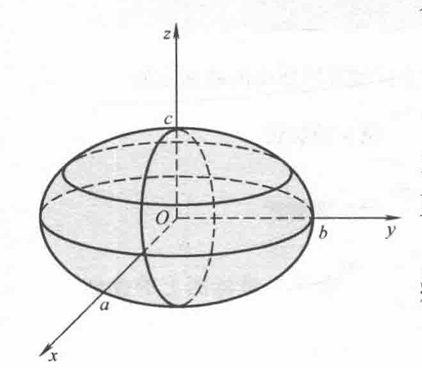
\includegraphics[width=0.95\linewidth,height=3.8cm,keepaspectratio]{Ellipsoid.png} \\
    单叶双曲面 &
    $\dfrac{x^2}{a^2}+\dfrac{y^2}{b^2}-\dfrac{z^2}{c^2}=1\ (a,b,c>0)$ &
    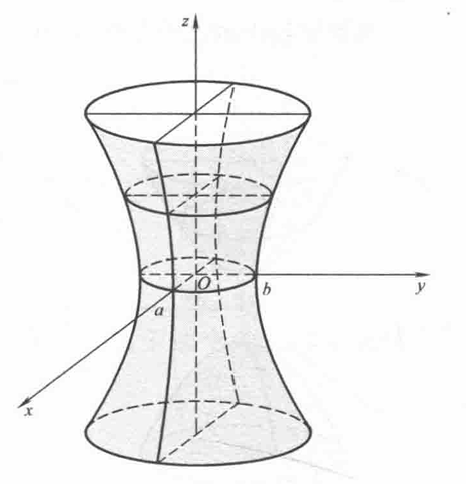
\includegraphics[width=0.95\linewidth,height=3.8cm,keepaspectratio]{Single-leaf_hyperbolic_surface.png} \\
    双叶双曲面 &
    $\dfrac{z^2}{c^2}-\dfrac{x^2}{a^2}-\dfrac{y^2}{b^2}=1\ (a,b,c>0)$ &
    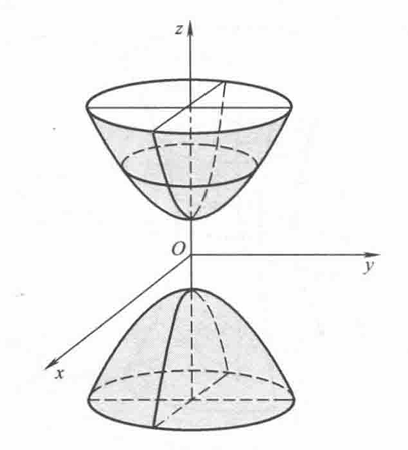
\includegraphics[width=0.95\linewidth,height=3.8cm,keepaspectratio]{Double-leaf_hyperbolic_surface.png} \\
    椭圆抛物面 &
    $z=\dfrac{x^2}{a^2}+\dfrac{y^2}{b^2}\ (a,b>0)$ &
    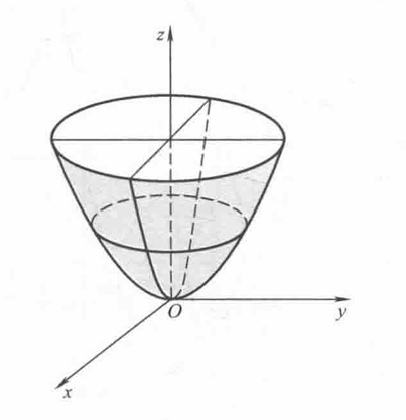
\includegraphics[width=0.95\linewidth,height=3.8cm,keepaspectratio]{Elliptic_paraboloid.png} \\
    双曲抛物面 &
    $z=\dfrac{x^2}{a^2}-\dfrac{y^2}{b^2}\ (a,b>0)$ &
    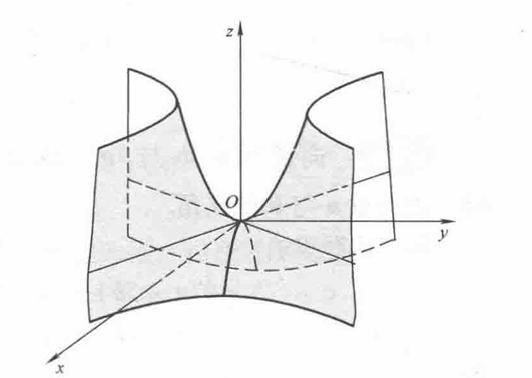
\includegraphics[width=0.95\linewidth,height=3.8cm,keepaspectratio]{Hyperbolic_paraboloid.png} \\
    \bottomrule
  \end{tabular}
  \caption{五种常见二次曲面}
\end{table}



总而言之，判断曲面类型时，最关键的其实不是原方程长什么样，而是化简后\textbf{平方项的符号结构}和\textbf{是否还保留线性项}。这里还有一个容易被略过去的点：经过平移与正交变换之后，我们并没有“改造”曲面本身，只是换了观察它的坐标系，所以标准式与原方程描述的是同一个几何对象。也正因如此，分类结果才有意义；否则我们整理出来的只会是一堆漂亮却无关的代数式。

我们来看一个例子，考虑二次曲面方程：
\[
x^2 + y^2 + 5z^2 - 6xy - 4x + 8y - 12z + 14 = 0.
\]

第一次看到它，你可能会觉得又是一堆项胡乱纠缠在一起，平方项、交叉项、一次项、常数项谁也不服谁。可是别忘了，数学里最迷人的时刻，往往就藏在表面杂乱无章的东西下面——关键是换一双眼睛去看。记
\[
\mathbf{x} = \begin{bmatrix} x \\ y \\ z \end{bmatrix},\quad
A = \begin{bmatrix}
1 & -3 & 0 \\
-3 & 1 & 0 \\
0 & 0 & 5
\end{bmatrix},\quad
\mathbf{b} = \begin{bmatrix} -2 \\ 4 \\ -6 \end{bmatrix},\quad d = 14.
\]
这里要注意交叉项的分配：方程中 \(-6xy\) 对应 \(2hxy\) 得 \(h=-3\)，没有 \(yz\) 和 \(zx\) 项，所以 \(f=g=0\)。于是原方程简洁地写作：
\[
\begin{bmatrix} x & y & z \end{bmatrix}
\begin{bmatrix}
1 & -3 & 0 \\
-3 & 1 & 0 \\
0 & 0 & 5
\end{bmatrix}
\begin{bmatrix} x \\ y \\ z \end{bmatrix}
+ 2\begin{bmatrix} -2 & 4 & -6 \end{bmatrix}
\begin{bmatrix} x \\ y \\ z \end{bmatrix}
+ 14 = \mathbf{x}^T A \mathbf{x} + 2\mathbf{b}^T \mathbf{x} + d = 0.
\]

写成这个样子以后，混乱感已经开始退去——原来那些散落在各处的系数，现在被收拢进了矩阵 \(A\) 和向量 \(\mathbf{b}\) 里。我们希望找到一个中心点 \(\mathbf{x}_0\) 使得一次项消失。解方程 \(A\mathbf{x}_0 + \mathbf{b} = \mathbf{0}\)，即
\[
\begin{cases}
x_0 - 3y_0 = 2,\\
-3x_0 + y_0 = -4,\\
5z_0 = 6.
\end{cases}
\]
解这个线性方程组，得到 \(\mathbf{x}_0 = \left(\frac{5}{4},\, -\frac{1}{4},\, \frac{6}{5}\right)^\mathrm{T}\)。令 \(\mathbf{x} = \mathbf{y} + \mathbf{x}_0\)，代入原方程。经过计算，新常数项变为
\[
d' = d + 2\mathbf{b}^T\mathbf{x}_0 + \mathbf{x}_0^T A \mathbf{x}_0 = 14 + 2(-2\cdot\frac{5}{4}+4\cdot(-\frac{1}{4})-6\cdot\frac{6}{5}) + \mathbf{x}_0^T A \mathbf{x}_0.
\]
平移后的方程为：
\[
\mathbf{y}^T A \mathbf{y} + \frac{33}{10} = 0 \quad \text{即} \quad \mathbf{y}^T A \mathbf{y} = -\frac{33}{10}.
\]
你看，所有一次项已经被吸收掉了。新坐标系的原点放在了曲面真正的中心——原来的方程看起来偏心，只是因为尺子没放对位置。

\(A\) 是实对称矩阵，它一定能被正交对角化。对角化的部分需要我们后面学习特征值与特征向量之后才可以做到，这部分内容在[P\label{quadratic}\pageref{diag}]，我们作为例题使用，这里直接给出对角化的结果是：

\[
P^T A P = \Lambda = \begin{bmatrix} 5 & 0 & 0 \\ 0 & 4 & 0 \\ 0 & 0 & -2 \end{bmatrix}.
\]
代入方程 \(\mathbf{y}^T A \mathbf{y} = -\frac{33}{10}\) 得：
\[
5u_1^2 + 4u_2^2 - 2u_3^2 = -\frac{33}{10}.
\]

两边乘以 \(-\frac{10}{33}\)，写成标准形式：
\[
-\frac{50}{33}u_1^2 - \frac{40}{33}u_2^2 + \frac{20}{33}u_3^2 = 1,
\]
或者等价地
\[
\frac{u_3^2}{33/20} - \frac{u_1^2}{33/50} - \frac{u_2^2}{33/40} = 1.
\]

两个平方项系数为负、一个为正，常数项为正，这正是\textbf{双叶双曲面}的特征。原来那团乱糟糟的代数藤蔓，经过平移和旋转之后，露出了它最质朴的面目：一个中心在原点的双叶双曲面。这印证了我们之前说的——曲面的本质不在于你最初用什么坐标去看它，而在于它平方项之间的符号结构。这里两个负一个正，曲面分成两片，无限延伸，正是双叶双曲面的性格。

当然后面还可以有一步操作就是把它化成规范型，具体操作就是抹除系数大小的信息，只保留正负号。这个操作是为了快速判断曲线的类型的，比如上面那个曲线的规范型就是：
\[
-z_1^2- z_2^2 + z_3^2 = 1.
\]

\begin{table}[htbp]
  \centering
  \renewcommand{\arraystretch}{1.4}
  \begin{tabular}{C{0.30\textwidth} C{0.60\textwidth}}
    \toprule
    曲面类型 & 规范型方程 \\
    \midrule
    椭球面 &
    $z_1^2 + z_2^2 + z_3^2 = 1$ \\
    单叶双曲面 &
    $z_1^2 + z_2^2 - z_3^2 = 1$ \\
    双叶双曲面 &
     $-z_1^2 - z_2^2 + z_3^2 = 1$ \\
    椭圆抛物面 &
    $ z_1^2 + z_2^2-z_3 =0$ \\
    双曲抛物面 &
    $ z_1^2 - z_2^2-z_3 =0$ \\
    \bottomrule
  \end{tabular}
  \caption{五种常见二次曲面的规范型}
\end{table}

我们看到其实曲面的类型本质上只由正系数的个数决定：全是正指数的方程是椭球；两个正系数的是单页双曲面；两个负系数的是双叶双曲面……于是数学上我们定义这样的系数叫做正惯性指数。这就引出了正定性这个概念。一个实对称矩阵 \(A\)（或者说它对应的二次型 \(f(\mathbf{x})=\mathbf{x}^T A\mathbf{x}\)）被称为\textbf{正定的}，如果对于任意非零向量 \(\mathbf{x}\in\mathbb{R}^n\)，都有 \(f(\mathbf{x})>0\)。换句话说，无论你朝哪个方向走，这个二次型的值都严格大于零，只在原点处才降为零。几何上看，这意味着 \(f(\mathbf{x})=1\) 的等值面是一个椭球，所有方向都被“拉向外侧”，没有哪个方向是向里凹的。正定性最核心的判定准则藏在特征值里：\(A\) 正定当且仅当它的所有特征值都大于零。原因很简单——通过正交变换（也就是旋转坐标系）把 \(A\) 对角化，得到 \(Q^T A Q = \operatorname{diag}(\lambda_1,\dots,\lambda_n)\)，此时二次型变成 \(\lambda_1 y_1^2+\cdots+\lambda_n y_n^2\)。要让这个和对于任何非零的 \((y_1,\dots,y_n)\) 都大于零，每个 \(\lambda_i\) 必须严格为正。一个更实操的办法是看顺序主子式：\(A\) 正定当且仅当它的各阶顺序主子式都大于零。这个法则在手算小规模矩阵时非常高效，但它本质上是特征值判据的推论，而不是替代。

与正定相对的，是\textbf{负定}：所有特征值小于零，二次型恒为负。介于两者之间的，是\textbf{半正定}（特征值非负，可以为零）和\textbf{半负定}（特征值非正）。如果一个矩阵的特征值既有正又有负，那就叫\textbf{不定}——它对应的二次型像马鞍一样，在某些方向向上弯曲，在另一些方向向下弯曲。这几种情况合在一起，恰好构成了对称矩阵在“符号”意义上的完整分类。你会发现，这个分类和之前讨论的惯性指数是一回事：正惯性指数 \(p\) 就是正特征值的个数，负惯性指数 \(q\) 就是负特征值的个数，而 \(r=p+q\) 就是矩阵的秩。正定对应 \(p=n\)，负定对应 \(q=n\)，半正定对应 \(p<n\) 且 \(q=0\)，不定对应 \(p>0\) 且 \(q>0\)。


\begin{itemize}
  \item \textbf{正定二次型}：正惯性指数 $p = n$（满秩，且所有系数为正）。  
  此时规范型为 $z_1^2 + z_2^2 + \cdots + z_n^2$。  
  \textbf{输出值特征}：对任意非零向量 $\mathbf{x}$，有 $f(\mathbf{x}) > 0$；几何上对应椭球面。

  \item \textbf{半正定二次型}：正惯性指数 $p < n$，且负惯性指数 $q = 0$（没有负平方项，但可能有零系数）。  
  规范型为 $z_1^2 + \cdots + z_p^2$（$p < n$）。  
  \textbf{输出值特征}：$f(\mathbf{x}) \ge 0$，且存在非零 $\mathbf{x}$ 使 $f(\mathbf{x}) = 0$；几何上对应“退化的”抛物柱面之类。

  \item \textbf{负定二次型}：正惯性指数 $p = 0$，负惯性指数 $q = n$（满秩且全负）。  
  规范型为 $-z_1^2 - z_2^2 - \cdots - z_n^2$。  
  \textbf{输出值特征}：对任意非零 $\mathbf{x}$，有 $f(\mathbf{x}) < 0$。

  \item \textbf{半负定二次型}：正惯性指数 $p = 0$，负惯性指数 $q < n$（没有正平方项，可能有零）。  
  规范型为 $ -z_1^2 - \cdots - z_q^2$。  
  \textbf{输出值特征}：$f(\mathbf{x}) \le 0$，且存在非零 $\mathbf{x}$ 使 $f(\mathbf{x}) = 0$。

  \item \textbf{不定二次型}：正惯性指数 $p > 0$ 且负惯性指数 $q > 0$。  
  \textbf{输出值特征}：$f(\mathbf{x})$ 既可正也可负（取决于方向），几何上对应双曲面或双曲抛物面。
\end{itemize}

于是判断系数矩阵$\mathbf{A}$的正定性可以直接告知我们其表征的几何形状，

可正定性为什么如此重要？原因不在定义本身，而在于它几乎无处不在。在优化中，一个多元函数的局部极小点，其海森矩阵必须是正定或半正定的——正定性直接告诉你这个临界点是不是真正的谷底。在统计学里，协方差矩阵天生就是半正定的，因为方差不可能为负。在物理中，弹性势能的二阶导数矩阵（刚度矩阵）正定时，系统才是稳定的；如果它不定，轻轻一推就会翻倒。甚至在机器学习里，核矩阵的正定性保证了优化问题的凸性，从而保证算法能找到全局最优解。换句话说，正定性是一种“能量符号”的检查：它回答的问题是，这个系统在每一个方向上，到底是抵制偏离（正定），还是放任甚至助长偏离（不定）？

如果你把矩阵想象成一个地形，正定的 \(A\) 就是一口碗——无论你从哪个方向离开原点，你都得往上爬。负定的 \(A\) 则是一个倒扣的碗，处处下坡。不定的 \(A\) 好比一个马鞍，沿着一条脊线向上，沿着另一条脊线向下。而半正定则像一条山谷——有些方向是平坦的，但不会有向下的方向。你看，这个分类并不抽象，它直接对应着物理直觉：稳定与不稳定，约束与自由，凸与凹。

判定一个具体矩阵是否正定，最直接的方法是检查它的特征值。但特征值计算往往代价较高，尤其当矩阵规模变大时。对于小矩阵，顺序主子式法则更便捷。还有一种常用的构造方式：若矩阵 \(A\) 可以写成 \(A = R^T R\) 且 \(R\) 列满秩，那么 \(A\) 自动正定——因为 \(\mathbf{x}^T A\mathbf{x} = \|R\mathbf{x}\|^2\)，而 \(R\mathbf{x}=0\) 当且仅当 \(\mathbf{x}=0\)。这种分解不仅给出了正定性的一个充分条件，还揭示了正定矩阵与内积之间的深层联系。事实上，任何一个正定矩阵都可以看作某个内积的度量矩阵：定义 \(\langle \mathbf{u},\mathbf{v}\rangle_A = \mathbf{u}^T A \mathbf{v}\)，它就成为一个合法的内积。从这个角度看，正定矩阵不过是“把标准点积换了一种尺度”而已——只要这个尺度在任何方向上都保持正性，就是正定的。

所以回到最初的问题：正定性究竟在说什么？它说的是，这个矩阵在任何方向上都不翻转符号。它像一杆秤，无论你从哪边称，重量都是正的。这种“方向无关的正性”看似苛刻，却恰恰是许多稳定系统、凸函数和概率结构的基石。就像一个房间里的温度分布，无论你朝哪个方向走，温度都在升高——那最低点一定就在你的脚下。正定性，正是那个告诉你“脚下就是谷底”的代数信使。


\subsection{解析几何}

现在我们拥有了这些观测这些曲面的初步视野，但是要解析这个曲面，如果总是解方程组的话，未免繁琐，那么有没有描述这些面更好的方法？

如何唯一确定一个平面？你的思绪或许会回溯到高中的那个下午，数学老师在黑板上口沫横飞的讲着立体几何，但是你只是望着窗外的树叶随风飘摆——没错！就是法向量，一个平面唯一由它的法向量确定。

但是怎么确定呢？平面里的所有线都是垂直于法向量的，但是我们只能描述点，如何用线描述点呢？没错，就是位矢！只要知道平面上的一个点$M_0(x_0,y_0,z_0)$，我们就可以根据这个点生成无数个向量，并根据垂直法向量$\mathbf{n}=(A,B,C)$约束这些生成向量的坐标：
\[
 \mathbf{n} \cdot (x-x_0,y-y_0,z-z_0) =0
\]

我们清楚的知道点积的运算法则，也就是说这个方程就是：
\[
  A(x-x_0)+B(y-y_0)+C(z-z_0)=0
\]
没错！这就是平面的方程，如果你将所有常数组合到一起，于是和我们上一章讨论的一样，平面的方程：
\[
  Ax+By+Cz+D=0
\]
就被这么构造出来了，这就是一般空间平面的一般式方程！

显然，我们之前的表述“一个平面唯一由它的法向量确定”并不完全正确，确切的说，它完全确定一类平面，这些平面互相平行，而具体确定一个平面还需要知道一个点。但我们是三维生物啊，我们知道三维空间长什么样子，要区别这些平行的平面，我们肯定不会看什么点啊什么乱七八糟的数学玩意，而是最返璞归真的观测平面间的距离，但是平面的距离怎么求呢？我们现在有一个平面$\pi$和一个点$M(x_0,y_0,z_0)$，现在要求点到平面的距离，怎么办？如果你上过高中你一定会，就是寻找平面上一个点和$M(x_0,y_0,z_0)$形成的向量在法向量上的投影，具体而言就是：
\[
 d(P,\pi)=\frac{|Ax_0+By_0+Cz_0+D|}{\sqrt{A^2+B^2+C^2}}.
\]

而直接计算两个平行的面的间距呢？就是把点$M(x_0,y_0,z_0)$的信息等价的换成平面方程中的信息罢了，还记得我们在点法式到一般式的过度吗，平面方程的参数$D$正是蕴含了关于经过点$M$的平面的一切信息，所以两个平行平面的间距只是：
\[
 d(P,\pi)=\frac{|D_1-D_2|}{\sqrt{A^2+B^2+C^2}}.
\]

之后我们便可以考虑构造直线了，在三维空间构造一个直线，最简单的方法就是拿两个平面相交一下，就得到了有两个约束方程的直线。这样求解出来的方程一般具有形式：
\[
  \frac{x-x_0}{a}=\frac{y-y_0}{b}=\frac{z-z_0}{c}.
\]
但是一直解方程肯定不是事，仿照我们考虑平面的思路，没错我们可以用向量，只不过我们用的不再是法向量，而是方向向量，在三维空间中，设直线 $l$ 过点 $P_0(x_0,y_0,z_0)$，方向向量为
$\mathbf{v}=(a,b,c)$（$\mathbf{v}\neq\mathbf{0}$），则有
\[
  (x,y,z)=(x_0,y_0,z_0)+t(a,b,c),\quad t\in\R,
\]

此外，过直线的平面方程可以表达为任意两平面方程的线性组合：
\[
  m(A_1x+B_1y+C_1z+D_1)+n(A_2x+B_2y+C_2z+D_2)=0
\]
这个源自于任意两个不共线的法向量可以作为这线性空间的基（线性代数部分会提到）。在高中学习圆锥曲线的时候，我就曾发现过这个规律，那时候虽然上课什么都没讲，但我已经悟到了所谓交点就是求两个约束方程的共解，当两个约束方程都知道后，就可以自然的生成无数经过这个点的线。这个好像是叫做“直线系方程”，真是有趣，很难想象那才是两年前，AI还不存在的时代。

\subsection{曲线和曲面}

既然一般二次曲面和直线平面我们已经了解了，那我们不由得思考：“弯曲的对象”呢？没错，弯曲的对象无法用一个向量描述，每一个坐标对应的向量可能都不一样，这时候你也许会想：那我岂不是给每一个坐标都规定一个向量就好了，这样点的运动就可以描述了，诶没错。这样你就发明了向量场！于是空间曲线可以被描述为：
\[
\mathbf{r}(t)=(x(t),y(t),z(t)),\quad t\in I.
\]


空间曲线最常见的局部几何对象就是\textbf{切线}和\textbf{法平面}。我们在二维空间中，切线的方程由曲线在点的导数和点的坐标决定，但是这无法普及到三维空间，因为三维空间有三个坐标，导数这一个只涉及两个对象的数学语言难以描述。

取曲线上一点 $P_0=\mathbf{r}(t_0)$。
当 $\mathbf{r}'(t_0)\neq\mathbf{0}$ 时，$\mathbf{r}'(t_0)$ 就是该点的切向量，因此切线可写为
\[
\ell:\ \mathbf{R}=\mathbf{r}(t_0)+s\,\mathbf{r}'(t_0),\quad s\in\mathbb{R}.
\]

法平面的意义可能是为了散度服务的，法平面是“垂直于切向量”的平面，描述这个平面必然会把法向量取为 $\mathbf{n}=\mathbf{r}'(t_0)$。于是法平面方程为
\[
\mathbf{r}'(t_0)\cdot\bigl((X,Y,Z)-\mathbf{r}(t_0)\bigr)=0,
\]

这就是我们描述曲线的切线和法向量的基本理论了，它很简单，但是我们遇到的问题却不一定这么简单。有时候我们并不知道曲线的具体表达式，而是以两个曲面的交线的形式描述一条曲线：
\[
\begin{cases}
F(x,y,z)=0,\\
G(x,y,z)=0.
\end{cases}
\]
若点 $P_0(x_0,y_0,z_0)$ 在交线上且梯度存在，则两个曲面的法向量分别是$\nabla F(P_0)$ 和$ \nabla G(P_0)$，那么交线在该点的切向量（方向向量）可取为
\[
\mathbf{v}=\nabla F(P_0)\times \nabla G(P_0).
\]
因此切线可以写成
\[
\ell:\ (X,Y,Z)=P_0+t\,\mathbf{v},\quad t\in\mathbb{R}.
\]

如果把它写成雅可比语言，等价于取
\[
\mathbf{v}=
\left(
\frac{\partial(F,G)}{\partial(y,z)},
\frac{\partial(F,G)}{\partial(z,x)},
\frac{\partial(F,G)}{\partial(x,y)}
\right)_{P_0},
\]
和叉积表达是同一个结论。

但是这样还是有问题，空间曲面呢？空间曲面怎么描述？

要想描述一个东西的本质，首先我们需要会构造它。构造一个曲面，肯定就是平移或者旋转二维曲线了，于是我们创造出两种空间曲面：
\begin{enumerate}
  \item \textbf{柱面（母线平行于某固定方向）}：
  当母线平行于 $z$ 轴时，柱面方程可写成
  \[
  F(x,y)=0,
  \]
  它与 $z$ 无关，表示把平面曲线 $F(x,y)=0$ 沿 作为母线的 $z$ 轴平移得到的曲面。
  更一般地，若柱面母线方向向量为 $\mathbf{v}$，可取两个与 $\mathbf{v}$ 垂直的线性函数
  $u=a_1x+b_1y+c_1z+d_1,\ v=a_2x+b_2y+c_2z+d_2$，则柱面可写为：
  \[
  \Phi(u,v)=0.
  \]

  \item \textbf{旋转曲面}：
  若母线在 $rz$ 平面上方程为 $F(r,z)=0$，绕 $z$ 轴旋转后得到，其余类型同理。
  \[
  F\!\left(\sqrt{x^2+y^2},z\right)=0,
  \]
\end{enumerate}

空间曲线当然可以用两个曲面方程的联立得到，不过那个有些复杂。

现在有了两类曲面，但是它们的形式还是太过于美好了一些，并非我们希望的统一工具，那看来这条路很难走通了，毕竟曲面的形式千千万，很难找到一个统一的构造法。

但是我们还是可以探究它的性质啊，也许可以有一些想法呢？

在点 $P_0$ 处，\textbf{切平面与曲面一阶近似重合}，其法向量就是曲面在该点的法向量。对于曲面 $F(x,y,z)=0$，若 $P_0$ 满足 $F(P_0)=0$ 且 $\nabla F(P_0)\neq\mathbf{0}$，则切平面方程是

\[
\nabla F(P_0)\cdot\bigl((X,Y,Z)-P_0\bigr)=0,
\]
法线（过 $P_0$ 且方向为法向量）可写为
\[
\frac{X-x_0}{F_x(P_0)}=\frac{Y-y_0}{F_y(P_0)}=\frac{Z-z_0}{F_z(P_0)}.
\]

显然完全没有任何值得探究的想法啊，难道真的就没有办法了吗？

\newpage

\section{基向量张成平面与曲面}

在线性代数还没发展起来的时代，我们只能向上面那样仿照二维笛卡尔空间讨论解析几何，当时随着线性代数蓬勃发展，我们发现空间是可以被线性表示的。从线性代数视角看，平面与曲面的核心都和“基向量如何张成”有关。

\subsection{两个基向量张成平面}

线性代数中提到，线性无关的基向量可张成一个向量空间，对于三维向量而言，这向量空间中的所有向量都可以具象化在三维空间的某个平面内，而对于零空间的向量，它们就表征的是空间中点的位矢，也就是点的坐标。这样我们就表示出所有过原点的平面了。而非零空间，也就是小节3.4.3中提到的仿射平面。构成仿射平面的向量并不能构成一个向量空间所以在线性代数部分我们并未过多的探讨它，但是在解析几何部分，我们可以简单的通过给定一点 $P_0$ 与两个不共线向量 $\mathbf{e}_1,\mathbf{e}_2$，就得到任何一个平面：
\[
\mathbf{X}(u,v)=\mathbf{P}_0+\begin{bmatrix}\mathbf{e}_1 & \mathbf{e}_2\end{bmatrix}\begin{bmatrix}u\\v\end{bmatrix},
\quad (u,v)\in\R^2.
\]
这说明平面本质上是二维参数空间到三维空间的线性嵌入，
$\mathbf{e}_1,\mathbf{e}_2$ 就是这个平面的基向量。


但除了简单的两种切平面描述之外，还有一种更通用的，就是利用矢量，显然曲面的矢量式我们是知道的：
\[
\mathbf{r}(u,v)=(x(u,v),y(u,v),z(u,v)),\quad P_0=\mathbf{r}(u_0,v_0).
\]
对于平面元上两个不共线的切向量，则切平面的法向量可取
\[
\mathbf{n}=\partial_u \mathbf{r}(u_0,v_0)\times \partial_v \mathbf{r}(u_0,v_0),
\]
切平面方程为
\[
\mathbf{n}\cdot\bigl((X,Y,Z)-P_0\bigr)=0.
\]

这是一个十分有趣的形式，你会发现平面和曲面之间并没有很大的区别，只不过它们的基向量有一些区别。我们考虑它们的矢量式：
\[
\mathbf{r}(u,v)=(x(u,v),y(u,v),z(u,v)),
\]
思索一下，如果三个坐标都是关于两个参量的线性函数，那么它是不是就是平面了？如果是非线性的，是不是就是曲面了？

\subsection{参数曲面由“变化的基向量”张成}

学习到这里时候我在想，如果二维平面可以被基向量张成那么平面是不是也可以呢？但是平面的基向量会随位置坐标而曲折，这就需要一个矩阵来参与进来拉伸旋转这些基向量。想到这里我猛然意识到，这不就是爱因斯坦场方程的度规张量！对参数曲面
\[
\mathbf{r}(u,v)=(x(u,v),y(u,v),z(u,v)),
\]
在每个点处都有两个切向量
\[
\mathbf{r}_u=\frac{\partial \mathbf{r}}{\partial u},\qquad
\mathbf{r}_v=\frac{\partial \mathbf{r}}{\partial v}.
\]
若 $\mathbf{r}_u\times\mathbf{r}_v\neq\mathbf{0}$，则它们线性无关并张成该点的切平面：
\[
T_{P}\Sigma=\mathrm{span}\{\mathbf{r}_u,\mathbf{r}_v\}.
\]
这些切平面可以包络出一个曲面，我们每次只需要考虑在切点处的微元就好了，那根据这个想法我们怎么描述基向量的变化呢？我们现在有两个切向量，那我们是否可以通过求切向量的变化率去预测呢？可以但是它没法任意生成曲面，并不直观。

怎么办呢？弯曲空间的坐标轴都是会改变的，即使向一个方向移动，基向量也会随着坐标的改变而改变，但是我们关心的只有方向不是么？我们可以让考虑的基向量都作为单位向量，这样我们就有了第一个不变量了——长度。

既然长度是不变量，那么这说明矩阵对在坐标轴上的量不存在拉伸作用，保证了基向量的归一化。那么显然这些量一定是在对角线上的，所以我们可以写出平面的变换：
\[
\operatorname{diag}\!\bigl(\mathbf{r}_1\!\cdot\!\mathbf{r}_1,\mathbf{r}_2\!\cdot\!\mathbf{r}_2,\ldots,\mathbf{r}_n\!\cdot\!\mathbf{r}_n\bigr)
\]
这个度规张量作用在一个基向量组上得到的还是它本身，至少是合理的不是？推而广之，对角项的意义不就是对坐标轴的拉伸？不过我们现在并不关心坐标轴刻度的变化，但是至少我们知道对角项的意义是距离的平方的拉伸。

然后我们就可以思考一下非对角元的作用了，显然它和曲面的几何量存在很大关系。现在我们采用的策略是使用点积制造不变量，那么根据自由组合定律我们可以先草拟一个二维度规：
\[
    g = 
    \begin{bmatrix} 
    g_{uu} & g_{uv} \\ 
    g_{vu} & g_{vv} 
    \end{bmatrix} = 
    \begin{bmatrix} 
    \mathbf{r}_u \cdot \mathbf{r}_u & \mathbf{r}_u \cdot \mathbf{r}_v \\ 
    \mathbf{r}_v \cdot \mathbf{r}_u & \mathbf{r}_v \cdot \mathbf{r}_v 
    \end{bmatrix}
\]

将这个度规矩阵作用于两个坐标增量向量 $\mathbf{a} = \begin{bmatrix} a_1 \\ a_2 \end{bmatrix}$ 和 $\mathbf{b} = \begin{bmatrix} b_1 \\ b_2 \end{bmatrix}$ 时，得到：

\[
    \langle \mathbf{a}, \mathbf{b} \rangle = \mathbf{a}^{\mathsf{T}} g \mathbf{b} = 
    \begin{bmatrix} a_1 & a_2 \end{bmatrix} 
    \begin{bmatrix} g_{11} & g_{12} \\ g_{21} & g_{22} \end{bmatrix} 
    \begin{bmatrix} b_1 \\ b_2 \end{bmatrix}
    = g_{11}a_1b_1 + g_{12}a_1b_2 + g_{21}a_2b_1 + g_{22}a_2b_2
\]
我们看到度规张量的分量在方程中就像一个权重，显然在基向量垂直的时候非对角元为零，可见非对角元描述了空间弯曲对内积的贡献权重，给出了它们在曲面切空间中的真实几何内积。度规张量 $g$ 的本质是一个将坐标微分映射为物理距离的二阶对称张量。
\begin{itemize}
    \item \textbf{对角项 ($g_{11}, g_{22}$)}：衡量了坐标轴在对应方向上的伸缩程度（归一化因子）。
    \item \textbf{非对角项 ($g_{12}, g_{21}$)}：衡量了坐标轴之间的夹角及扭曲程度（由于内积满足交换律，故 $g_{12} = g_{21}$，矩阵必须对称）。
\end{itemize}

于是弧长元与面积元分别为
\[
ds^2=E\,du^2+2F\,du\,dv+G\,dv^2,
\qquad
dS=\|\mathbf{r}_u\times\mathbf{r}_v\|\,du\,dv=\sqrt{EG-F^2}\,du\,dv.
\]

所以度规直接决定长度、角度与面积等几何量。

\newpage

\section{统一思想：n维体的边界包裹出n+1维体的内部}

在数学物理中，有一条贯穿始终的几何直觉：\textbf{低维的边界，包裹着高维的内部}。一条闭合曲线围出一块平面区域；一个封闭曲面包裹出一块空间区域；一个$n$维的有向流形，它的边界是一个$n-1$维的闭流形。这种“包裹”关系，是积分学中最深刻的纽带。

当我们计算一个量在边界上的累积时，往往可以转化为计算它的某种“变化率”在内部区域的累积。这就是\textbf{斯托克斯定理}的统一形式：
\[
\int_{\partial \Omega} \omega = \int_{\Omega} d\omega.
\]
其中$\Omega$是一个$n+1$维的区域，$\partial\Omega$是它的$n$维边界，$\omega$是一个$n$阶微分形式，$d\omega$是它的外微分。

这个公式像一把钥匙，打开了从曲线到曲面、从曲面到区域的所有积分转化之门：

\begin{itemize}
    \item 当$n=1$时，它是\textbf{格林公式}：边界曲线上的环量，等于内部区域的旋度积分。
    \item 当$n=2$且$\Omega$为曲面时，它是\textbf{斯托克斯公式}：边界曲线上的环量，等于曲面上旋度的通量。
    \item 当$n=2$且$\Omega$为立体区域时，它是\textbf{高斯公式}（散度定理）：边界曲面上的通量，等于内部散度的体积分。
\end{itemize}

本文将从最朴素的“投影原理”出发，逐步揭示这一统一思想在具体计算中的实现方式——无论是弯曲的曲线还是扭曲的曲面，我们都可以通过投影到平坦的参数空间，用拉伸因子将复杂的几何转化为简单的重积分。最终你会发现，所有那些看似繁复的积分公式，不过是同一个几何直觉在不同坐标系下的倒影。

\subsection{曲线积分的投影原理}
\label{path-independent}
现在从面降到线。思路一模一样：一条空间曲线 $C$ 是弯的，要沿着它累积什么量，我们就把它``拉直''——投影到一个参数轴上去，通常选时间 $t$。

曲线由参数方程 $\mathbf{r}(t) = (x(t), y(t), z(t))$ 给出。曲线上一个微小的弧长元素 $ds$，和参数 $t$ 的微小增量 $dt$ 之间，又有一个拉伸关系。这个关系由曲线的切向量长度给出：
\[
ds = \left| \frac{d\mathbf{r}}{dt} \right| dt = \sqrt{\left(\frac{dx}{dt}\right)^2 + \left(\frac{dy}{dt}\right)^2 + \left(\frac{dz}{dt}\right)^2} \, dt
\]
这就是曲线积分的投影原理：弧长元素等于参数轴上线元 $dt$ 乘以``速度''大小这个拉伸因子。

\begin{wrapfigure}{l}{0.32\textwidth}
  \begin{center}
    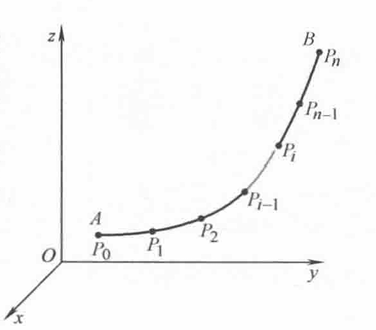
\includegraphics[width=0.3\textwidth]{line_integeal1.png}
  \end{center}
    \caption{第一类曲线积分}
    \label{fig:line_integeal1}
    \vspace{5pt}
\end{wrapfigure}
第一类曲线积分，就是对\textbf{标量场的路径积分}。物理上，如果一根弯曲的金属丝有线密度 $\lambda(x,y,z)$，总质量就是：
\[
M = \int_C \lambda \, ds
\]
把 $ds$ 换成那个带速度大小的 $dt$，把所有坐标换成 $t$ 的函数，积分就变成了关于参数 $t$ 的普通定积分。弯曲再一次被吞进了拉伸因子。吱吱吱吱吱吱吱吱吱吱吱吱吱吱吱吱吱吱吱吱吱吱吱吱吱吱吱吱吱吱吱吱吱吱吱吱吱吱吱吱吱吱吱吱吱吱吱吱吱吱吱吱吱吱吱吱吱吱吱吱吱吱吱吱吱吱吱吱吱吱吱吱吱吱吱吱吱吱吱吱吱吱吱吱吱吱吱吱吱吱吱吱吱吱吱吱吱吱吱吱吱吱吱吱吱吱吱吱吱吱吱吱吱吱吱吱吱吱

\begin{wrapfigure}{r}{0.32\textwidth}
  \begin{center}
    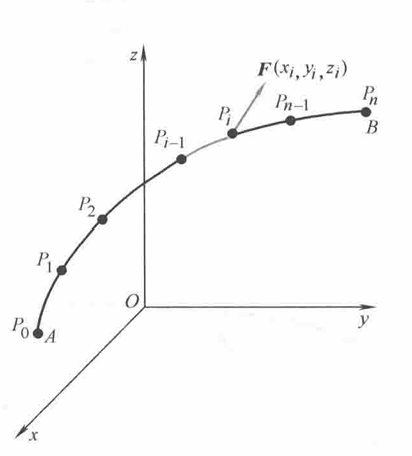
\includegraphics[width=0.3\textwidth]{line_integeal2.png}
  \end{center}
    \caption{第二类曲线积分}
    \label{fig:line_integeal2}
    \vspace{15pt}
\end{wrapfigure}

第二类曲线积分，是算一个\textbf{标量场$\mathbf{F}$的路径积分}。这次我们用有向弧元 $d\mathbf{r}$，它是切线方向乘以弧长：$d\mathbf{r} = \mathbf{T} \, ds$，其中 $\mathbf{T}$ 是单位切向量。但这里有个更直接的写法。注意到：
\[
d\mathbf{r} = \frac{d\mathbf{r}}{dt} dt
\]
这个切向量本身就包含了方向和拉伸两部分信息。因此第二类曲线积分：
\[
\int_C \mathbf{F} \cdot d\mathbf{r} = \int_{t_A}^{t_B} \mathbf{F}(\mathbf{r}(t)) \cdot \frac{d\mathbf{r}}{dt} dt
\]


我们看到，再次不需要单独处理弧长 $ds$ 和方向 $\mathbf{T}$，参数化一写，所有几何信息全被速度矢量 $d\mathbf{r}/dt$ 打包带走。积分号下不过是矢量场分量与速度分量的一对一乘积之和，在 $t$ 轴上老老实实地积分。

所以，整个故事惊人地统一：无论曲面还是曲线，无论第一类还是第二类，你做的无非是把弯曲的几何对象投影到平坦的参数空间，算出一个拉伸因子或者有向投影因子，然后一切就都变成了简单平凡的多重积分。弯曲世界的秘密，就是这么被拉平的。

\begin{wrapfigure}{r}{0.32\textwidth}
  \begin{center}
    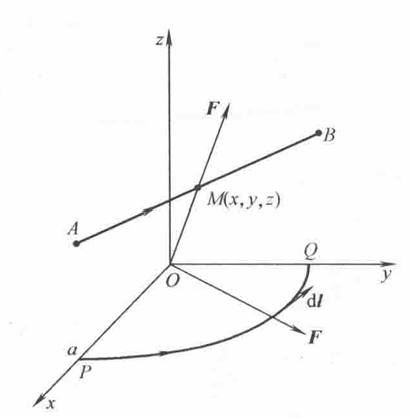
\includegraphics[width=0.3\textwidth]{line_integeal2-xyz.png}
  \end{center}
    \caption{直角坐标系下曲线积分}
    \label{fig:line_integeal2-xyz}
    \vspace{15pt}
\end{wrapfigure}

直角坐标系是最直白的情形，但它仍然完美服从这个投影逻辑。设空间曲线用参数 $t$ 写出 $\mathbf{r}(t) = (x(t), y(t), z(t))$，那么速度矢量为 $\dot{\mathbf{r}} = (\dot{x}, \dot{y}, \dot{z})$，拉伸因子就是
\[
\left|\frac{d\mathbf{r}}{dt}\right| = \sqrt{\dot{x}^2 + \dot{y}^2 + \dot{z}^2}.
\]
第一类曲线积分直接代入即得
\[
\int_C f \, ds = \int_{t_A}^{t_B} f(x(t), y(t), z(t)) \, \sqrt{\dot{x}^2 + \dot{y}^2 + \dot{z}^2} \, dt.
\]
第二类曲线积分同样是把矢量场 $\mathbf{F} = (P, Q, R)$ 与速度矢量做点乘：
\[
\int_C \mathbf{F} \cdot d\mathbf{r} = \int_{t_A}^{t_B} \left[ P \dot{x} + Q \dot{y} + R \dot{z} \right] dt.
\]
弯曲被彻底消化在 $\dot{x}, \dot{y}, \dot{z}$ 这些导数里，积分号下只剩 $t$ 的一元函数。




极坐标系处理平面曲线，当曲线本身直接用辐角 $\theta$ 作为参数时，事情反而变得更干净。此时参数方程写为$\mathbf{r}(\theta) = (r(\theta)\cos\theta,\; r(\theta)\sin\theta)$,其中 $r(\theta)$ 是极径关于辐角的函数。对参数 $\theta$ 求导，速度矢量（确切地说是切向量）为
\[
\frac{d\mathbf{r}}{d\theta} = \left( r'(\theta)\cos\theta - r(\theta)\sin\theta,\; r'(\theta)\sin\theta + r(\theta)\cos\theta \right).
\]
计算它的长度平方：
\[
\left|\frac{d\mathbf{r}}{d\theta}\right|^2 = (r'\cos\theta - r\sin\theta)^2 + (r'\sin\theta + r\cos\theta)^2= r'^2 + r^2.
\]
因此以 $\theta$ 为参数的拉伸因子为
\[
ds = \sqrt{r'^2 + r^2} \, d\theta,
\]
这个结果有一种朴素的美感：弧长元素在极坐标下以 $\theta$ 为自变量时，就是径向变化率 $r'$ 与当前位置 $r$ 的平方和开根号——前者告诉你曲线正在向外或向内跑得多快，后者告诉你即使 $r$ 不变，角向扫过的弧长本身就是 $r d\theta$。两者正交，各自的贡献以勾股定理叠加。

第一类曲线积分随之化为对 $\theta$ 的普通定积分：
\[
\int_C f \, ds = \int_{\theta_A}^{\theta_B} f(r(\theta), \theta) \, \sqrt{r'^2 + r^2} \, d\theta.
\]
被积函数里的 $f$ 照旧取曲线上的点坐标，弧长微元被拉伸因子全部吸收，弯曲再一次消失在积分号下。

第二类曲线积分同样简洁。当矢量场在极坐标基下写为 $\mathbf{F} = F_r \hat{\mathbf{r}} + F_\theta \hat{\boldsymbol{\theta}}$ 时，微位移沿曲线的表达式为$d\mathbf{r} = dr \, \hat{\mathbf{r}} + r d\theta \, \hat{\boldsymbol{\theta}}
        = \left( r' \hat{\mathbf{r}} + r \hat{\boldsymbol{\theta}} \right) d\theta$，
因此第二类曲线积分化为
\[
\int_C \mathbf{F} \cdot d\mathbf{r} = \int_{\theta_A}^{\theta_B} \left[ F_r(r(\theta),\theta) \, r'(\theta) + F_\theta(r(\theta),\theta) \, r(\theta) \right] d\theta.
\]
这里把 $\theta$ 作为参数的意义看得最清楚：径向分量 $F_r$ 与 $r'$ 配对，角向分量 $F_\theta$ 与 $r$ 配对，二者相加之后老老实实对 $\theta$ 积分。弧长微元的方向信息和拉伸信息全部被 $r'\hat{\mathbf{r}} + r\hat{\boldsymbol{\theta}}$ 这个切向量打包带走，积分号下不再有任何几何负担，只剩下关于 $\theta$ 的一元函数。投影原理在此处变得几乎透明：弯曲的曲线被参数 $\theta$ 拉直，拉伸因子 $\sqrt{r'^2+r^2}$ 和切向量 $r'\hat{\mathbf{r}}+r\hat{\boldsymbol{\theta}}$ 分别负责第一类和第二类积分中所需的全部几何信息。


柱坐标系是极坐标向空间的一层自然延伸。令参数化为 $r(t), \theta(t), z(t)$，直角坐标由 $x = r\cos\theta$，$y = r\sin\theta$，$z = z$ 给出。速度分量现在多了一个 $\dot{z}$：
\[
\dot{x} = \dot{r} \cos\theta - r \dot{\theta} \sin\theta, \quad
\dot{y} = \dot{r} \sin\theta + r \dot{\theta} \cos\theta, \quad
\dot{z} = \dot{z}.
\]
速度大小平方是三者各自贡献之和：
\[
\dot{x}^2 + \dot{y}^2 + \dot{z}^2 = \dot{r}^2 + r^2 \dot{\theta}^2 + \dot{z}^2.
\]
拉伸因子因此为
\[
\left|\frac{d\mathbf{r}}{dt}\right| = \sqrt{\dot{r}^2 + r^2 \dot{\theta}^2 + \dot{z}^2}.
\]
第一类曲线积分据此写出：
\[
\int_C f \, ds = \int_{t_A}^{t_B} f(r(t), \theta(t), z(t)) \, \sqrt{\dot{r}^2 + r^2 \dot{\theta}^2 + \dot{z}^2} \, dt.
\]
第二类曲线积分则在柱坐标基 $(\hat{\mathbf{r}}, \hat{\boldsymbol{\theta}}, \hat{\mathbf{z}})$ 下进行。设矢量场分量为 $F_r, F_\theta, F_z$，微位移在柱坐标下的表达式是
\[
d\mathbf{r} = dr \, \hat{\mathbf{r}} + r d\theta \, \hat{\boldsymbol{\theta}} + dz \, \hat{\mathbf{z}}.
\]
因此
\[
\mathbf{F} \cdot d\mathbf{r} = F_r \, dr + F_\theta \, r d\theta + F_z \, dz
    = \left[ F_r \dot{r} + F_\theta \, r \dot{\theta} + F_z \dot{z} \right] dt.
\]
于是
\[
\int_C \mathbf{F} \cdot d\mathbf{r} = \int_{t_A}^{t_B} \left[ F_r \dot{r} + F_\theta \, r \dot{\theta} + F_z \dot{z} \right] dt.
\]
竖直方向干干净净，径向与角向则完全沿用了极坐标的结构。弯曲的几何信息再一次被全部收纳进三个速度分量与那个由位置决定的拉伸因子 $r$ 中。

球坐标系是最复杂的情形，但投影思路一如既往。参数化为 $r(t), \theta(t), \phi(t)$，直角坐标的对应关系是
\[
x = r \sin\theta \cos\phi, \quad
y = r \sin\theta \sin\phi, \quad
z = r \cos\theta.
\]
对 $t$ 求导，速度分量为
\[
\begin{aligned}
\dot{x} &= \dot{r} \sin\theta \cos\phi + r \dot{\theta} \cos\theta \cos\phi - r \dot{\phi} \sin\theta \sin\phi, \\
\dot{y} &= \dot{r} \sin\theta \sin\phi + r \dot{\theta} \cos\theta \sin\phi + r \dot{\phi} \sin\theta \cos\phi, \\
\dot{z} &= \dot{r} \cos\theta - r \dot{\theta} \sin\theta.
\end{aligned}
\]
若老老实实去算 $\dot{x}^2 + \dot{y}^2 + \dot{z}^2$，交叉项全部奇迹般消去，剩下三个相互正交的贡献：
\[
\left|\frac{d\mathbf{r}}{dt}\right|^2 = \dot{r}^2 + r^2 \dot{\theta}^2 + r^2 \sin^2\theta \, \dot{\phi}^2.
\]
拉伸因子取平方根：
\[
\left|\frac{d\mathbf{r}}{dt}\right| = \sqrt{\dot{r}^2 + r^2 \dot{\theta}^2 + r^2 \sin^2\theta \, \dot{\phi}^2}.
\]
第一类曲线积分于是为
\[
\int_C f \, ds = \int_{t_A}^{t_B} f(r(t), \theta(t), \phi(t)) \, \sqrt{\dot{r}^2 + r^2 \dot{\theta}^2 + r^2 \sin^2\theta \, \dot{\phi}^2} \, dt.
\]
第二类曲线积分同样沿着球坐标基矢 $(\hat{\mathbf{r}}, \hat{\boldsymbol{\theta}}, \hat{\boldsymbol{\phi}})$ 展开。微位移在球坐标下的形式是
\[
d\mathbf{r} = dr \, \hat{\mathbf{r}} + r d\theta \, \hat{\boldsymbol{\theta}} + r \sin\theta \, d\phi \, \hat{\boldsymbol{\phi}}.
\]
设矢量场分量为 $F_r, F_\theta, F_\phi$，则
\[
\mathbf{F} \cdot d\mathbf{r} = F_r \, dr + F_\theta \, r d\theta + F_\phi \, r \sin\theta \, d\phi.
\]
化为参数积分：
\[
\int_C \mathbf{F} \cdot d\mathbf{r} = \int_{t_A}^{t_B} \left[ F_r \dot{r} + F_\theta \, r \dot{\theta} + F_\phi \, r \sin\theta \, \dot{\phi} \right] dt.
\]
径向拉伸系数为 $1$，极角方向的拉伸系数为 $r$，方位角方向的拉伸系数为 $r \sin\theta$。和曲面上的面积元素如出一辙，这些拉伸因子正是从参数空间 $(r,\theta,\phi)$ 投射到真实空间时，各坐标方向上的几何缩放率。弯曲的球面、弯曲的路径，所有这些一度让人感到棘手的几何，最后不过是在被导数和系数规整之后，安安静静地躺在一个关于 $t$ 的定积分里。整个故事的核心没有变过：参数化把曲线拉直，拉伸因子把弯曲吃掉，积分于是归为平凡。

\begin{table}[htbp]
\centering
\caption{曲线积分的投影原理：各坐标系下的积分公式}
\medskip
\label{tab:curve_integral}
\renewcommand{\arraystretch}{1.6}
\begin{tabular}{p{2.8cm}|p{6.5cm}|p{6.5cm}}
\toprule
\textbf{坐标系} & \textbf{第一类曲线积分 $\int_C f \, ds$} & \textbf{第二类曲线积分 $\int_C \mathbf{F} \cdot d\mathbf{r}$} \\
\midrule
一般参数\;$(t)$ & $\displaystyle \int_{t_A}^{t_B} f(\mathbf{r}(t)) \left| \frac{d\mathbf{r}}{dt} \right| dt$ & $\displaystyle \int_{t_A}^{t_B} \mathbf{F}(\mathbf{r}(t)) \cdot \frac{d\mathbf{r}}{dt} dt$ \\
\midrule
直角坐标\;$(t)$ & $\displaystyle \int_{t_A}^{t_B} f \sqrt{\dot{x}^2 + \dot{y}^2 + \dot{z}^2} \, dt$ & $\displaystyle \int_{t_A}^{t_B} \left( P\dot{x} + Q\dot{y} + R\dot{z} \right) dt$ \\
\midrule
极坐标\;$(\theta)$ & $\displaystyle \int_{\theta_A}^{\theta_B} f \sqrt{r'^2 + r^2} \, d\theta$ & $\displaystyle \int_{\theta_A}^{\theta_B} \left( F_r r' + F_\theta r \right) d\theta$ \\
\midrule
柱坐标\;(t) & $\displaystyle \int_{t_A}^{t_B} f \sqrt{\dot{r}^2 + r^2 \dot{\theta}^2 + \dot{z}^2} \, dt$ & $\displaystyle \int_{t_A}^{t_B} \left( F_r \dot{r} + F_\theta r \dot{\theta} + F_z \dot{z} \right) dt$ \\
\midrule
球坐标\;(t) & $\displaystyle \int_{t_A}^{t_B} f \sqrt{\dot{r}^2 + r^2 \dot{\theta}^2 + r^2 s_\theta^2 \dot{\phi}^2} \, dt$ & $\displaystyle \int_{t_A}^{t_B} \left( F_r \dot{r} + F_\theta r \dot{\theta} + F_\phi r s_\theta \dot{\phi} \right) dt$ \\
\bottomrule
\end{tabular}
\end{table}

这张表格本身就是投影原理最凝练的注脚。第一列是坐标系的名称，它们不过是参数空间的不同选法；第二列是第一类曲线积分，核心永远是“标量函数 $\times$ 拉伸因子”；第三列是第二类曲线积分，核心永远是“矢量场分量 $\times$ 有向速度分量”。无论曲线弯成什么样子，无论你选择哪种坐标语言去描述它，所有几何信息都被收纳进那几个导数与拉伸系数之中，积分号下最终只剩一个老老实实的定积分。弯曲世界的秘密，就是这样在参数轴上被一寸一寸拉平的。

前面我们花了很大力气说明一件事：弯曲的曲线可以通过参数化拉直，曲线积分最终都化成了参数轴上的定积分。但曲线积分还有另一个同样深刻的归宿——它不一定非要用参数 $t$ 来算。在某些条件下，一个沿闭合曲线的积分，可以转化为曲线所围区域上的二重积分。这就是格林公式。它在精神上和投影原理完全一致：把边界上弯弯绕绕的东西，投影到它围住的平坦区域里去，让二维的平面区域来承担所有的计算。

\begin{figure}[H]
    \centering
    \begin{subfigure}[b]{0.3\textwidth}
        \centering
        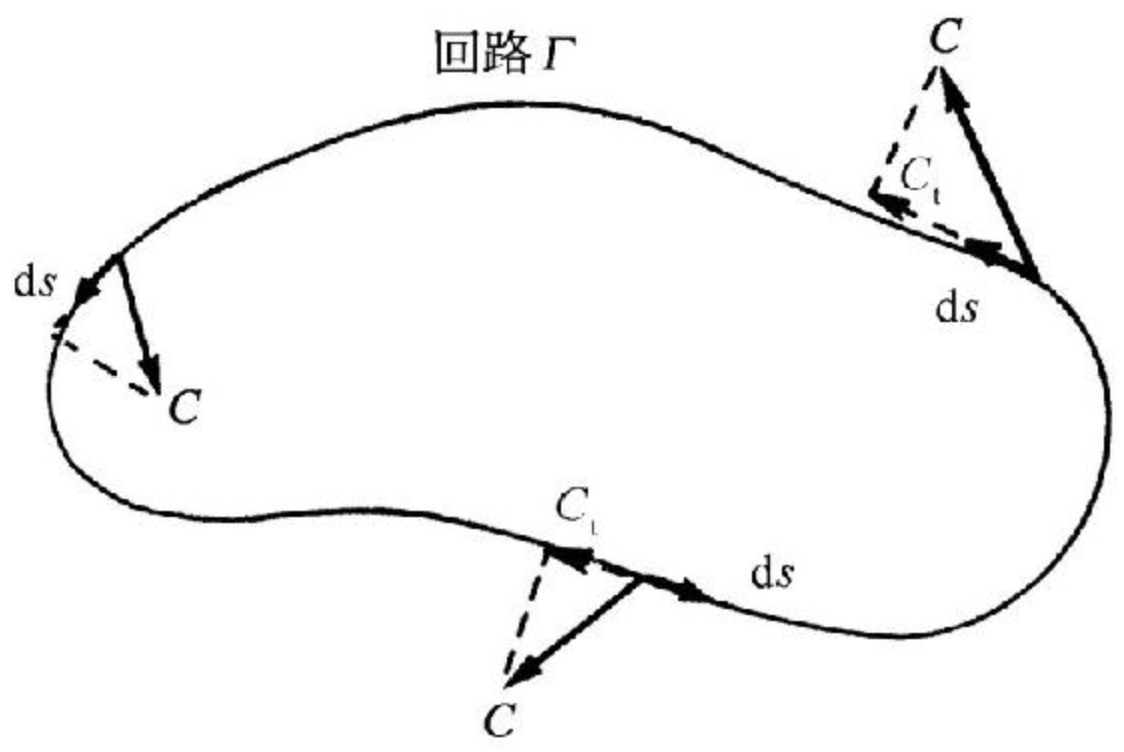
\includegraphics[width=0.7\textwidth]{circleintegral.png}
        \caption{任意回路}
        \label{fig:c1}
    \end{subfigure}
    \hfill
    \begin{subfigure}[b]{0.3\textwidth}
        \centering
        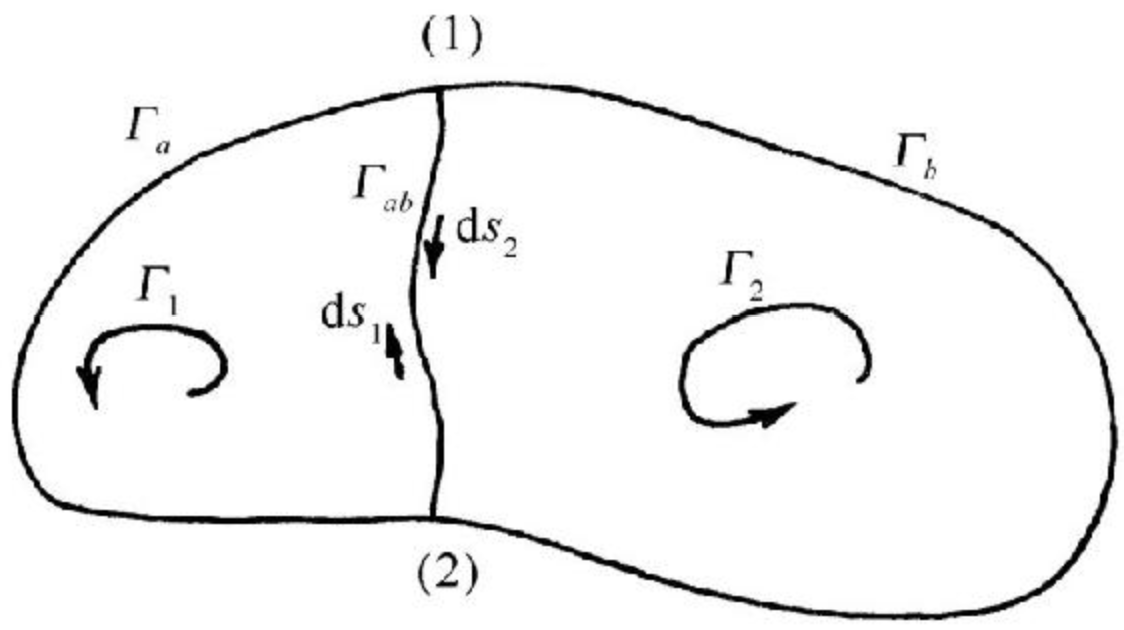
\includegraphics[width=0.7\textwidth]{circleintegral2.png}
        \caption{一分为二的任意回路}
        \label{fig:c2}
    \end{subfigure}
    \hfill
    \begin{subfigure}[b]{0.3\textwidth}
        \centering
        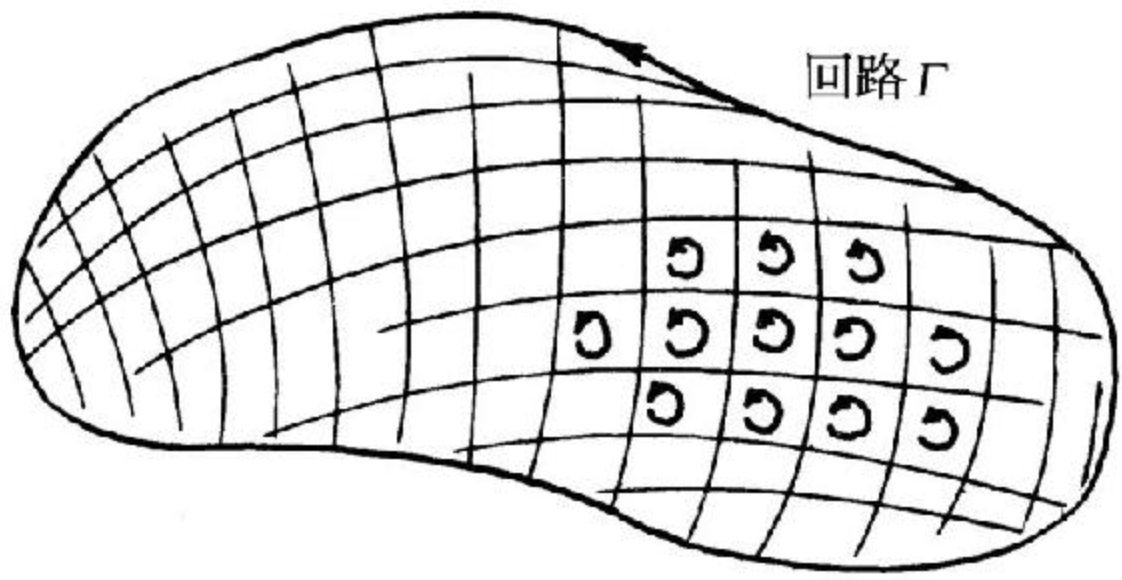
\includegraphics[width=0.7\textwidth]{circleintegraln.png}
        \caption{分割成无数小回路}
        \label{fig:cn}
    \end{subfigure}
    \caption{不断分割回路}
    \label{fig:combined}
\end{figure}

我们现在考虑任意回路$\Gamma$，对一个任意的向量$\mathbf{C}$环积分。现在我们在回路上任取两点(1)和(2)，在两点建建立一个新的曲线，那么我们就将原来的$\Gamma$分割为$\Gamma_1$和$\Gamma_2$。我们同样以逆时针对两个环路积分，我们发现在(1)和(2)连线上的路径积分恰好相抵，所以整个积分值不变。

以此类推，我们继续将这个环路分割成无数小环路$\Gamma_i$，那么根据我们上面的讨论，对所有$\Gamma_i$积分后结果和直接积分$\Gamma$是一样的。这就是最基本的微元分割法，将不规则的任意曲折环路分割成无数规则的小正方块，从而另辟蹊径，化繁为简，解决问题。


\begin{wrapfigure}{L}{0.32\textwidth}
  \begin{center}
    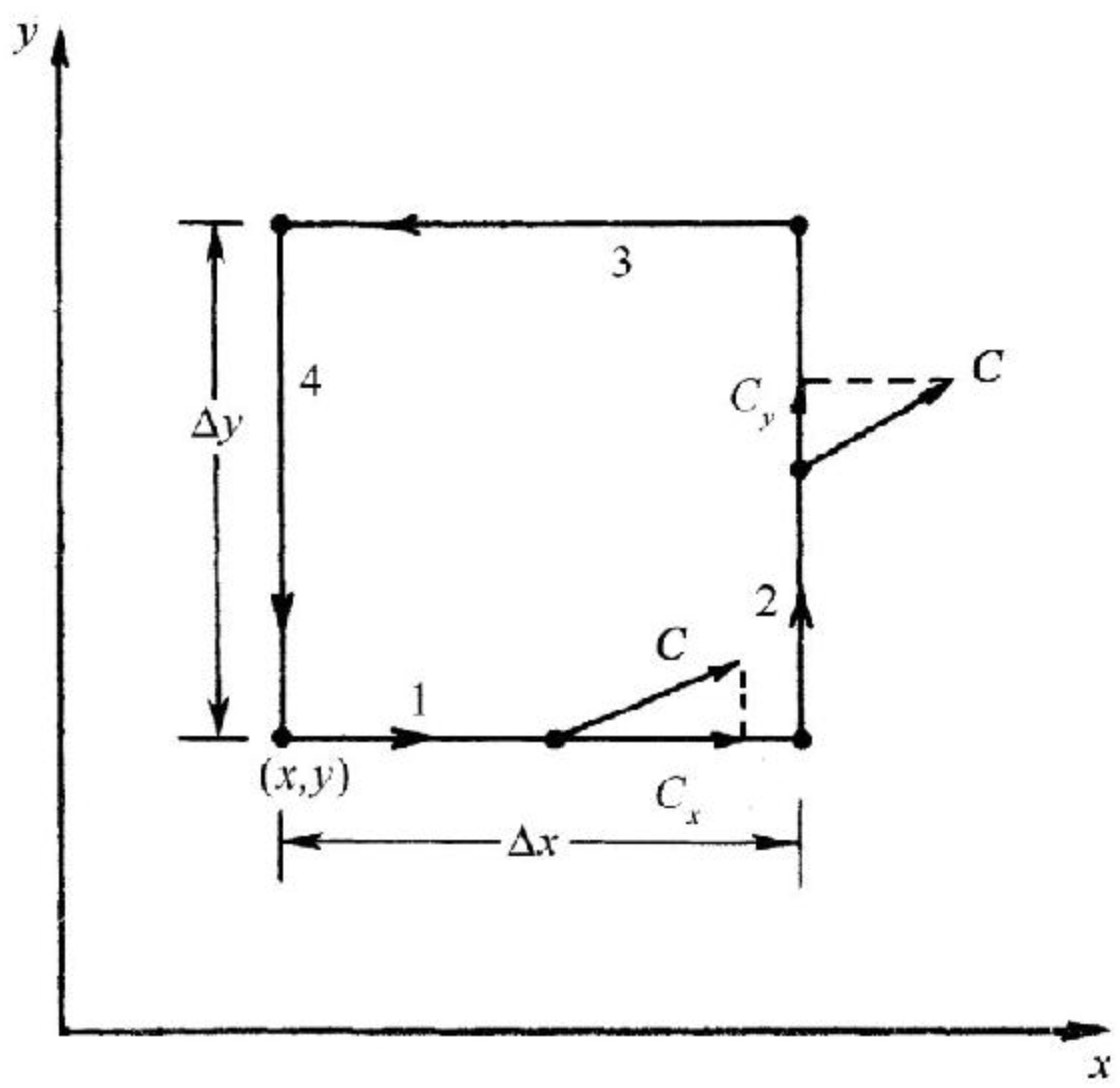
\includegraphics[width=0.3\textwidth]{circleintegralsquare.png}
  \end{center}
    \caption{小正方形环积分}
    \label{fig:squc}
\end{wrapfigure}

这样我们就可以通过只讨论一个小正方形的环路积分结果，然后反推整体了，一个小正方形微元，对于任意的向量场$\mathbf{C}(P,Q)$，我们不难写出它的路径积分的完整结果就是：
\[
\oint_C P \, dx + \oint_C Q \, dy 
\]

但是这个结果显然并不能令我们满意，我们要继续化简它。考虑到两个积分是对称的，所以我们先只考虑$\oint_C P \, dx $，这个积分是怎么回事呢？我们沿着路径一步步写下来，发现其实只有路径1和路径3对积分结果有贡献，所以显然：

\[
\oint_C P \, dx = \int P(x,y) dx - \int P(x,y+\Delta y) dx
\]

\bigskip

这时候熟悉导数定义的你可能已经看出一些端倪了，如果我们把原式稍微做一些改写，那么你就会发现：

\[
\int (P(x,y) - P(x,y+\Delta y) )dx = - \int \left[ \int \frac{\partial P}{\partial y} \, dy \right] dx= - \iint_D \frac{\partial P}{\partial y} \, dx\,dy.
\]

这个式子最后就变成了一个面积分！补全剩下的部分，我们得到：

\[
\iint_D (\frac{\partial Q}{\partial x}-\frac{\partial P}{\partial y}) \, dx\,dy 
\]

你会发现，面积分的母函数就是这个向量场的旋度！
\[
\iint_D (\nabla \times \mathbf{C}) \, dx\,dy 
\]

它的物理图像现在已经十分清晰。取一个极小的矩形回路，面积 $\Delta x \Delta y$，粗略算出沿其边界的环量就是小回路所包围的“微观旋转”。把一个宏观区域划分成无数这样的小方格，相邻方格之间边界上的积分方向相反，相互抵消，留下来的只有最外圈边界上的环量。内部所有微观旋转的总和，就这样一层层传递到了边界。格林公式不过是这个直觉的精确写法：边界上的大回路循环，是内部所有微小循环的加总。

它也为我们提供了一种选择策略：给定一个曲线积分，我们有两种办法——要么老老实实参数化把它拉直，要么用格林公式把它变成内部的二重积分。哪条路好算选哪条。如果积分路径是闭合的，被积函数又比较简单，格林公式往往把问题直接降维打击：二重积分比参数化绕圈算起来舒服得多。

格林公式最常写出的形式是上面那个关于环量的：
\[
\oint_C P \, dx + Q \, dy = \iint_D \left( \frac{\partial Q}{\partial x} - \frac{\partial P}{\partial y} \right) dx\,dy.=\iint_D (\nabla \times \mathbf{C}) \, dx\,dy 
\]
这被称为格林公式的切向形式，因为它处理的是矢量场沿边界切线方向的分量。

如果把二维矢量场看作三维矢量场在前两维的投影，它的旋度只有 $z$ 分量，即 $(\nabla \times \mathbf{F})_z$。于是格林公式可以写成
\[
\oint_C \mathbf{F} \cdot d\mathbf{r} = \iint_D (\nabla \times \mathbf{F}) \cdot \mathbf{n} \, dx\,dy.
\]
这就是斯托克斯公式，是一种更全面的描述。


\subsection{曲面积分的投影原理}

假设你有一块曲面 $S$，它在空间里弯来扭去。现在你想把某个依赖于位置的量 $f(x,y,z)$ 在这块曲面上累积起来。直接算没法算，因为曲面是弯的。但大自然给了我们一个极聪明的办法：把这块曲面压扁，投影到一个你熟悉的平面上，比如 $xy$ 平面。

\begin{wrapfigure}{L}{0.32\textwidth}
  \begin{center}
    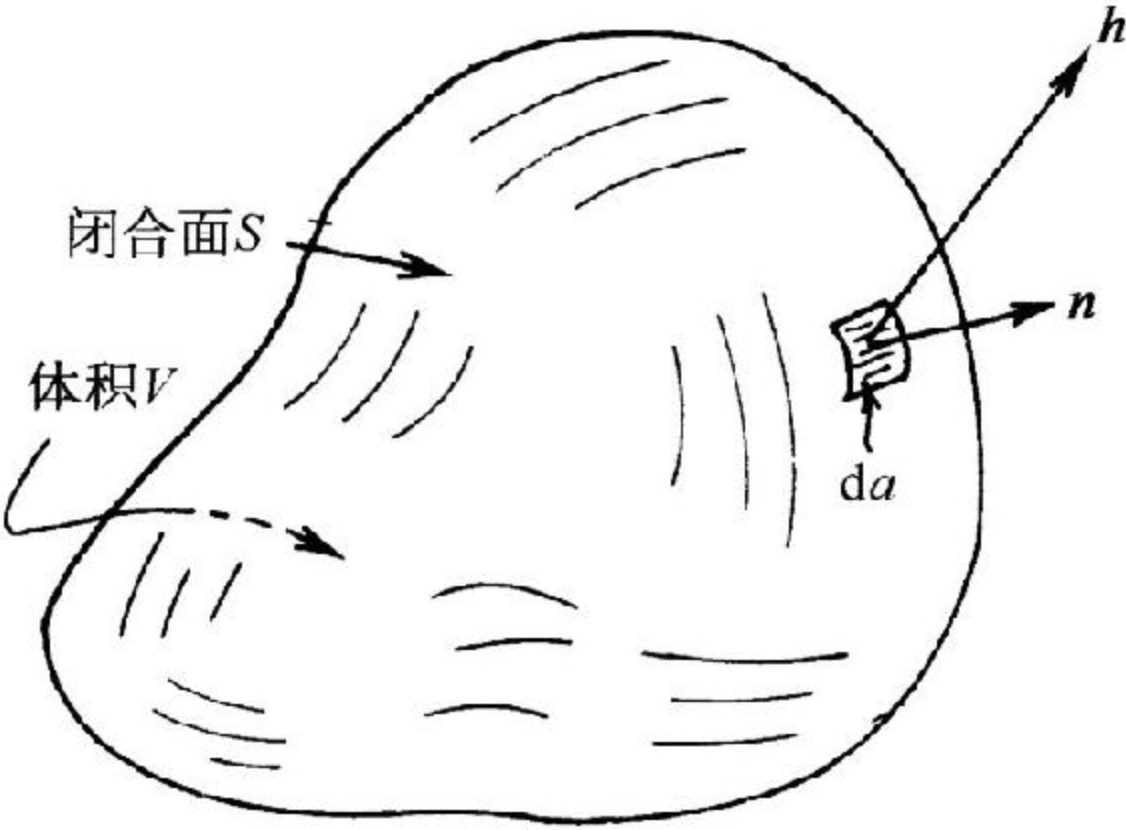
\includegraphics[width=0.3\textwidth]{closurface.png}
  \end{center}
    \caption{小正方形环积分}
    \label{fig:closurface}
\end{wrapfigure}

我们从最朴素的地方开始。在曲面上取一个微小的矩形面元 $dS$，把它投影到 $xy$ 平面上，得到一个影子，就是熟悉的小矩形 $dx\,dy$。这两个面积之间差了多少？你拿一张纸，把它倾斜，它在桌面上的投影面积就变小了。变小的比例就是倾斜角的余弦。设曲面的单位法向量为 $\mathbf{n}$，$xy$ 平面的单位法向量是 $\mathbf{k} = (0,0,1)$，那么：
\[
dx\,dy = dS \, |\mathbf{n} \cdot \mathbf{k}| = dS \, |\cos\theta|
\]
其中 $\theta$ 是法向量与垂直轴之间的夹角。反过来，曲面上的微小面积就是：
\[
dS = \frac{dx\,dy}{|\mathbf{n} \cdot \mathbf{k}|}
\]
如果曲面很平，几乎水平，$\mathbf{n}$ 近似垂直，$\cos\theta \approx 1$，那么 $dS \approx dx\,dy$。如果曲面很陡，几乎垂直，$\cos\theta$ 很小，投影面积就远远小于实际面积，$dS$ 比 $dx\,dy$ 大得多。这个分母 $|\mathbf{n} \cdot \mathbf{k}|$ 就是我们的拉伸因子。

现在把曲面漂亮地写成一个标量函数的等值面：$F(x,y,z)=0$。曲面上任意一点的法向量天然就是 $F$ 的梯度 $\nabla F$，它指向等值面变化最快的方向，也就是严格垂直于曲面的方向。单位法向量因此就是：
\[
\mathbf{n} = \frac{\nabla F}{|\nabla F|}
\]
把这个代入刚才的夹角余弦：
\[
\mathbf{n} \cdot \mathbf{k} = \frac{\nabla F}{|\nabla F|} \cdot (0,0,1) = \frac{F_z}{|\nabla F|}
\]
其中 $F_z = \partial F / \partial z$。于是我们就得到了从投影面积到曲面面积的转换公式：
\[
dS = \frac{dx\,dy}{|\mathbf{n} \cdot \mathbf{k}|} = \frac{|\nabla F|}{|F_z|} \, dx\,dy
\]
这个式子非常漂亮：右边的 $|\nabla F|/|F_z|$ 就是拉伸因子。它恰好是两个梯度量的比值，分子是法向量的全长，分母是法向量在 $z$ 轴上的投影长度。它们的比值刚好补偿了投影带来的面积收缩。这就是投影原理的核心：曲面上翘起的小块面积，等于它在平面上投影的面积，乘以这个由梯度比值决定的拉伸因子。

第一类曲面积分，就是把某个标量函数在曲面上累积。物理上常常是质量，或者电荷。如果面密度是 $\rho(x,y,z)$，那么总质量就是：
\[
M = \iint_S \rho \, dS
\]
一旦用投影原理把 $dS$ 换成 $(|\nabla F|/|F_z|) \, dx\,dy$，再根据 $F(x,y,z)=0$ 把被积函数里的 $z$ 用 $x,y$ 表达，这个积分就变成了在 $xy$ 投影区域 $D$ 上的普通二重积分：
\[
M = \iint_D \rho \, \frac{|\nabla F|}{|F_z|} \, dx\,dy
\]
弯的变成平的，秘密全在梯度的比值里。

第二类曲面积分，本质上是计算一个矢量场 $\mathbf{A}$ 穿过曲面 $S$ 的净流量。这里要小心：矢量场穿过一个面元，只和垂直于面元的分量有关。所以我们不用面元的纯面积 $dS$，而用有向面元 $d\mathbf{S} = \mathbf{n} \, dS$。流量就是 $\mathbf{A} \cdot d\mathbf{S}$。

梯度的语言让这件事格外优雅。把 $\mathbf{n} = \nabla F / |\nabla F|$ 和 $dS = (|\nabla F|/|F_z|) \, dx\,dy$ 同时代入，绝妙的事情发生了——$|\nabla F|$ 在上下的乘积中爽快地约掉：
\[
d\mathbf{S} = \mathbf{n} \, dS = \frac{\nabla F}{|\nabla F|} \cdot \frac{|\nabla F|}{|F_z|} \, dx\,dy = \frac{\nabla F}{|F_z|} \, dx\,dy
\]
有向面元就是梯度本身除以 $|F_z|$，再乘以投影面积元。通常我们取定投影区域的定向，把绝对值写进积分限，有向面元就是：
\[
d\mathbf{S} = \frac{\nabla F}{F_z} \, dx\,dy
\]
投影把面积和方向这两个信息同时编码进了梯度矢量与 $F_z$ 的比值里。于是第二类曲面积分：
\[
\iint_S \mathbf{A} \cdot d\mathbf{S} = \iint_D \mathbf{A} \cdot \frac{\nabla F}{F_z} \, dx\,dy
\]
又是一个平直区域上的普通二重积分。流量的计算，其实是矢量场分量与梯度分量之间的一场点积运算，在参数平面上干净利落地完成。


上面我们看到，第二类曲面积分通过梯度的语言，被干净利落地转化成了投影区域上的二重积分：
\[
\iint_S \mathbf{A} \cdot d\mathbf{S} = \iint_D \mathbf{A} \cdot \frac{\nabla F}{F_z} \, dx\,dy.
\]
这已经很漂亮了，但费曼可能会歪着头问：\emph{“如果我们不是仅仅算一张曲面的流量，而是算一个闭合曲面——比如一个气泡、一个盒子、或者一个土豆形状的东西——的总流量，有没有更聪明的办法？”}

\begin{wrapfigure}{L}{0.32\textwidth}
  \begin{center}
    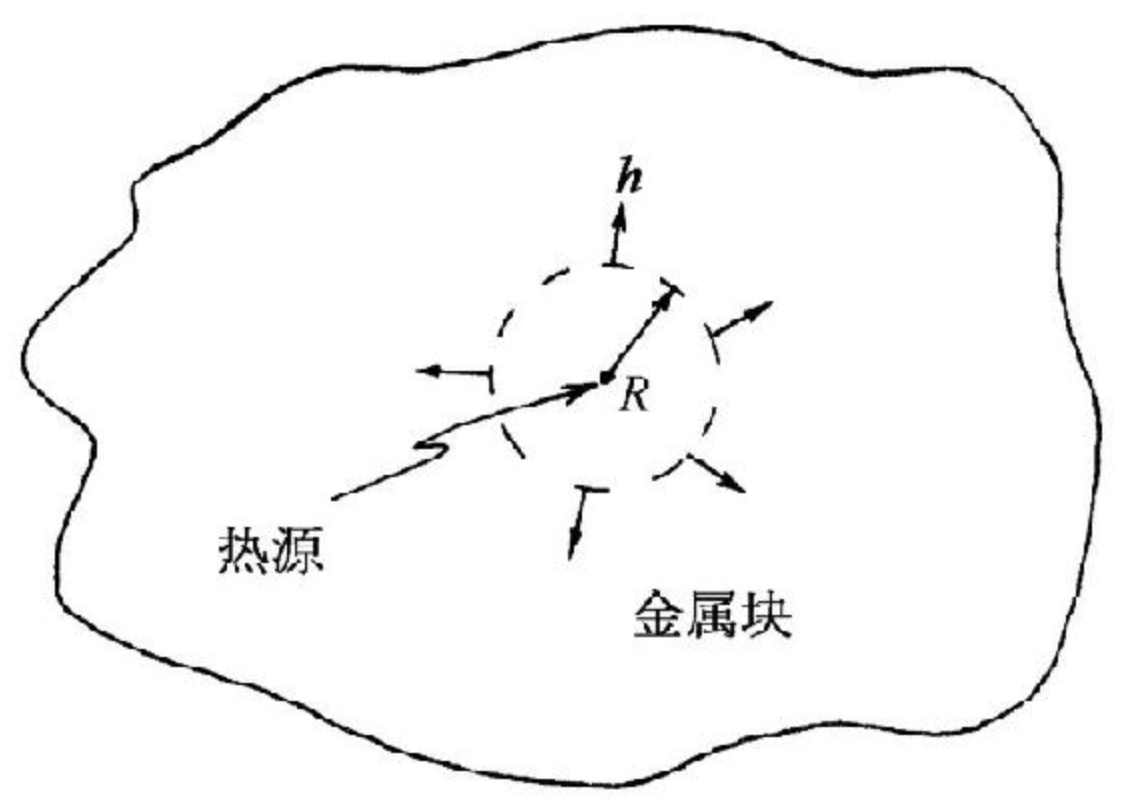
\includegraphics[width=0.3\textwidth]{flux.png}
  \end{center}
    \caption{小正方形环积分}
    \label{fig:closurface}
\end{wrapfigure}

答案是肯定的。而且这个办法会引出一个贯穿整个电磁学和流体力学的重要公式：\textbf{高斯公式}，也叫做散度定理。设想一个闭合曲面 $S$，它围出了一个三维区域 $V$。我们想计算矢量场 $\mathbf{A}$ 穿过这个闭合曲面的\textbf{净流量}——也就是流出去的减去流进来的。费曼可能会这样描述：\emph{“你在这块区域的边界上架设了一层细密的筛网，测量每一滴流体是跑出去还是钻进来，然后把所有结果加起来。”}

这个净流量，跟区域内部发生的事情密切相关。如果在区域内部的某一点，矢量场像一个小喷泉一样向外发散，那它对净流量的贡献就是正的；如果像一个小漏斗一样向内汇聚，贡献就是负的；如果只是单纯地流过而没有源头或陷阱，贡献就是零。

\begin{wrapfigure}{R}{0.32\textwidth}
  \begin{center}
    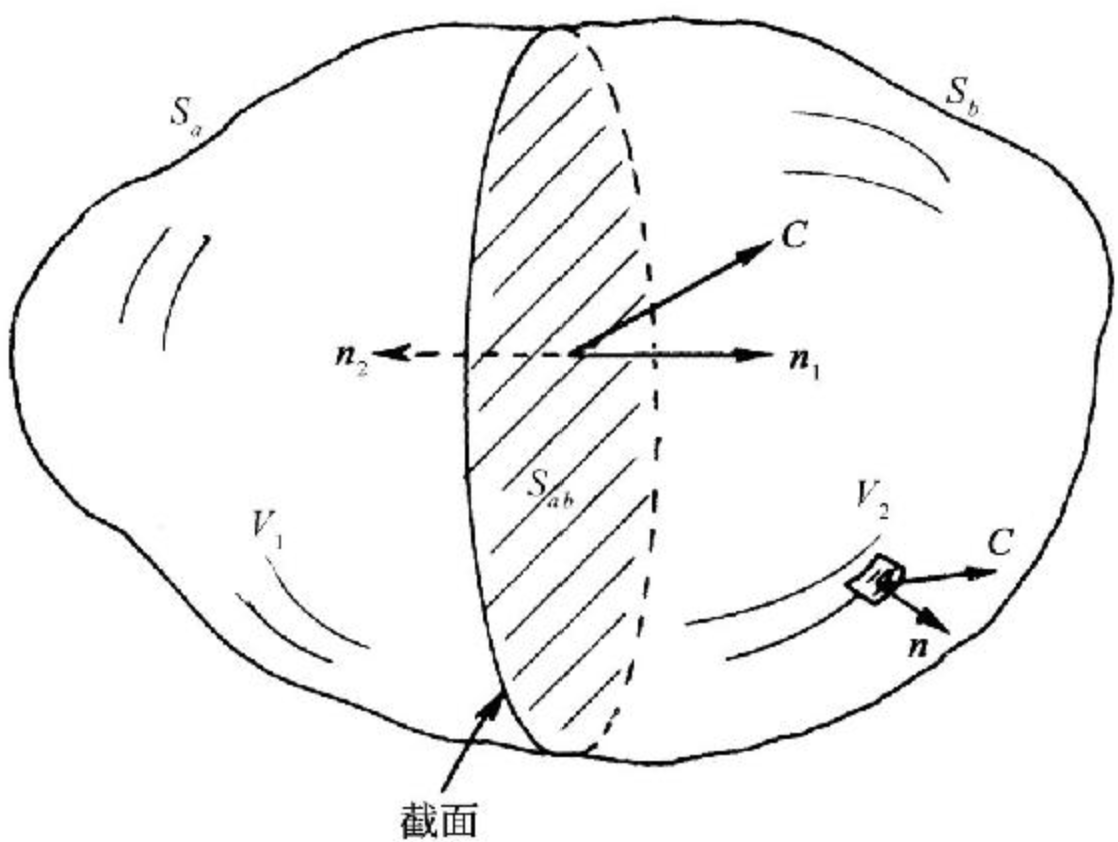
\includegraphics[width=0.3\textwidth]{divsurf.png}
  \end{center}
    \caption{小正方形环积分}
    \label{fig:closurface}
\end{wrapfigure}

但是我们该怎么描述这个想法呢？和格林公式如出一辙：我们把这个闭合的三维区域切成两块，比如分成 $V_1$ 和 $V_2$，它们的边界曲面分别是 $S_1$ 和 $S_2$，而公共截面则出现了两次。这时，一个绝妙的抵消发生了——在公共截面上，$S_1$ 的外法向与 $S_2$ 的外法向恰好相反，因此分别计算 $S_1$ 和 $S_2$ 上的通量再相加时，截面的贡献正好一正一负，爽快地抵消为零。剩下的部分拼起来，恰好就是原来那个闭合曲面 $S$ 上的总通量。所以说，先分割再求和，与直接对整个 $S$ 积分，结果完全一样。你看，这和格林公式切割平面区域时，内部线段上的线积分相互抵消的情形，是不是一模一样？多么有趣，这些方法论竟然在不同维度下达成了惊人的统一！


\begin{wrapfigure}{L}{0.32\textwidth}
  \begin{center}
    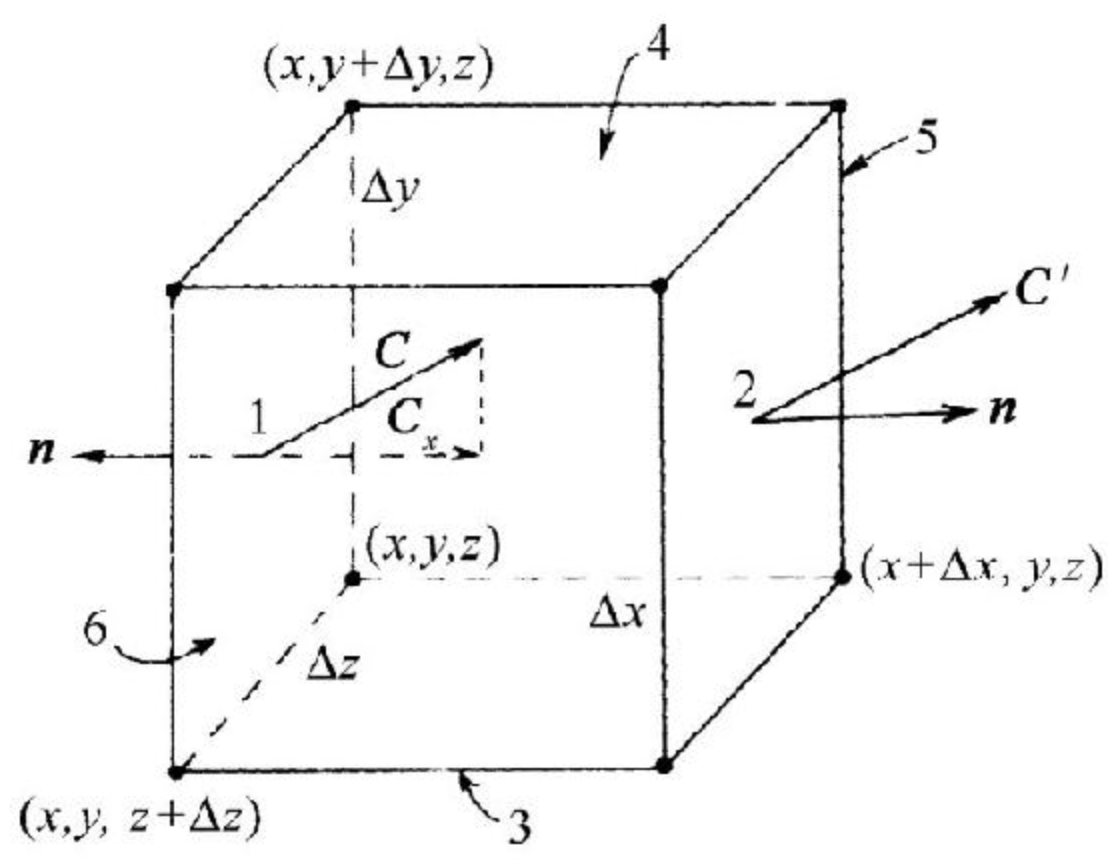
\includegraphics[width=0.3\textwidth]{suqflux.png}
  \end{center}
    \caption{小正方形环积分}
    \label{fig:closurface}
    \vspace{10pt}
\end{wrapfigure}


于是乎，我们就可以把任意一个复杂的三维体切割成无数个小正方体来讨论。考虑三个方向是对称的，所以我们以 $x$ 方向为例。对于矢量场 $\mathbf{C}$ 在面1和面2上的通量，就是：
\[
\mathbf{C}(x+\Delta x,y,z) \cdot \mathbf{n}\,\Delta y \Delta z \;+\; \mathbf{C}(x,y,z) \cdot (-\mathbf{n}\,\Delta y \Delta z).
\]
这个式子，是不是像之前一样，可以稍稍改写？
\[
\mathbf{C}(x+\Delta x,y,z) - \mathbf{C}(x,y,z) = \frac{\partial \mathbf{C}}{\partial x}\,\Delta x.
\]
于是，$x$ 方向上一对相对面贡献的净通量约为 
\[
\frac{\partial C_x}{\partial x}\,\Delta x \Delta y \Delta z.
\]
同理，$y$ 方向和 $z$ 方向也给出类似的表达式。把三个方向的贡献加起来，就得到这个小正方体总共的净通量：
\[
\left( \frac{\partial C_x}{\partial x} + \frac{\partial C_y}{\partial y} + \frac{\partial C_z}{\partial z} \right) \Delta V,
\]
其中 $\Delta V = \Delta x \Delta y \Delta z$ 是小正方体的体积。


这个表达式启发我们定义一个叫做\textbf{散度}的量，记作 $\nabla \cdot \mathbf{A}$。它是一个\textbf{标量场}，在每一点上的数值可以理解为：\emph{围绕该点取一个无穷小的体积，测量穿过这个小体积边界的净流量，再除以这个微小体积。}换句话说，散度就是“单位体积的净流出量”。

费曼可能会用他标志性的手势比划：\emph{“你取一粒灰尘那么小的小方块，看看有多少东西从它的六个面跑出来，再除以小方块的体积。当你把小方块缩得越来越小，这个比值会趋近于一个确定的数——这就是那一点的散度。”}


把上面这个小正方体的结果，对全部分割的小体求和，所有内部截面上的通量都会因为相邻小体法向相反而是相互抵消（就像格林公式中内部线段上的抵消一样），只剩下最外层边界曲面 $S$ 上的总通量。于是我们就得到了高斯公式：
\[
\iint_{S} \mathbf{A} \cdot d\mathbf{S} = \iiint_{V} (\nabla \cdot \mathbf{A}) \, dV.
\]
左边是矢量场穿过闭合曲面 $S$ 的净流量（边界上的总和），右边是散度在内部区域 $V$ 上的三重积分（内部源头强度的总和）。费曼会拍着桌子说：\emph{“看！外面发生了什么，完全由内部的总源头决定。你不需要真的绕着那个讨厌的曲面一格一格地算——你只需要钻进里面，把散度加起来就行了！”}



“散度”这个名字起得极其贴切。如果 $\nabla \cdot \mathbf{A} > 0$，表示该点是“源”，流体从这里\textbf{散}发出去；如果 $\nabla \cdot \mathbf{A} < 0$，表示该点是“汇”，流体向这里\textbf{汇聚}；如果 $\nabla \cdot \mathbf{A} = 0$，表示该点没有源头也没有陷阱，流进来的和流出去的一样多，也就是\textbf{无源场}（比如磁场）。


有趣的是，我们前面用梯度把有向面元写成 $d\mathbf{S} = (\nabla F / F_z) \, dx\,dy$ 的那个技巧，在高斯公式的证明中也扮演了角色。你可以把闭合曲面分成上下两半，分别用投影法计算，然后惊讶地发现：那些 $F_z$ 在分母上的项，经过微积分基本定理的魔力，最后变成了对 $A_z$ 的偏导数的积分——这正是散度的一部分。

高斯公式统一了三种偏导数：
\[
\nabla \cdot \mathbf{A} = \frac{\partial A_x}{\partial x} + \frac{\partial A_y}{\partial y} + \frac{\partial A_z}{\partial z}.
\]
每一个偏导数项，都来自对应方向上的“进出差额”。费曼可能会总结：\emph{“数学家的聪明之处在于，他们把边界上的复杂测量，转化成了内部一个简单的加法。你只需要知道‘每一点的喷泉有多强’，然后把它们全部加起来——就这么简单。”}


\subsection{结语}

我们一路从曲线到曲面，从投影到拉伸，从参数化到格林公式，始终在做同一件事：把弯曲或者复杂的几何对象上的积分，转化成更简单、更平坦的对象上的积分。这种转化的极致，出现在一个更宏大的观念里——\textbf{斯托克斯定理}的现代形式。

这个观念极其简单，却又极其深邃：\textbf{一个微分形式在区域边界上的积分，等于它的外微分在区域内部的积分}。用符号写出来，就是：
\[
\int_{\partial \Omega} \omega = \int_{\Omega} d\omega.
\]

这里的 $\Omega$ 是一个 $n+1$ 维的区域，$\partial \Omega$ 是它的边界——一个 $n$ 维的闭曲面（或闭曲线）。$\omega$ 是一个 $n$ 阶微分形式，$d\omega$ 是它的外微分，是一个 $n+1$ 阶微分形式。边界 $\partial \Omega$ 的定向由 $\Omega$ 的定向诱导。

这句话包含了我们见过的一切：

\begin{itemize}
    \item 当 $n=1$，$\Omega$ 是二维平面区域，$\partial \Omega$ 是它的边界曲线，$\omega = P\,dx + Q\,dy$，$d\omega = \left( \frac{\partial Q}{\partial x} - \frac{\partial P}{\partial y} \right) dx \wedge dy$，上式就是\textbf{格林公式}：
    \[
    \oint_{\partial \Omega} P\,dx + Q\,dy = \iint_{\Omega} \left( \frac{\partial Q}{\partial x} - \frac{\partial P}{\partial y} \right) dx\,dy.
    \]

    \item 当 $n=2$ 且 $\Omega$ 是三维空间中的一块曲面，$\partial \Omega$ 是它的边界曲线，$\omega = P\,dx + Q\,dy + R\,dz$，$d\omega$ 是它的旋度分量组成的二阶形式，上式就是\textbf{斯托克斯公式}：
    \[
    \oint_{\partial \Omega} P\,dx + Q\,dy + R\,dz = \iint_{\Omega} \left[ \left( \frac{\partial R}{\partial y} - \frac{\partial Q}{\partial z} \right) dy\wedge dz + \cdots \right] = \iint_{\Omega} (\nabla \times \mathbf{F}) \cdot \mathbf{n} \, dS.
    \]

    \item 当 $n=2$ 且 $\Omega$ 是三维空间中的一块立体区域，$\partial \Omega$ 是它的封闭边界曲面，$\omega = P\,dy\wedge dz + Q\,dz\wedge dx + R\,dx\wedge dy$，$d\omega = \left( \frac{\partial P}{\partial x} + \frac{\partial Q}{\partial y} + \frac{\partial R}{\partial z} \right) dx\wedge dy\wedge dz$，上式就是\textbf{高斯公式}（散度定理）：
    \[
    \iint_{\partial \Omega} \mathbf{F} \cdot d\mathbf{S} = \iiint_{\Omega} (\nabla \cdot \mathbf{F}) \, dV.
    \]
\end{itemize}

这个统一公式的威力在于：它把 \textbf{“边界上的累积”} 与 \textbf{“内部的总和”} 之间的等价性，提炼成了一个不可再分的几何真理。无论你面对的是曲线、曲面还是三维区域，无论你计算的是流量、环量还是通量，本质上都是同一件事情：\textbf{高维的内部效应，投影为低维的边界行为}。

回到我们最初的“投影原理”：把曲面投影到平面上，把曲线投影到参数轴上，无非是这种统一思想在具体坐标系下的操作。而斯托克斯定理，则是这个思想在最抽象、最本质层面上的宣告——所有的积分，归根结底，都是边界在说话。

\chapter{微积分}

第一节主要是介绍了极限的定义以及相关运算。

极限的定义一般只有考试会考，所以只要会做题就好。它的核心就是如何放缩 $|f(x)-L|$，使得可以找到一个简单的 $\delta(\varepsilon)$ 使得 $|x-a|<\delta$ 成立；你不必考虑多么精确，只要简单且正确就好。

极限的性质基本只会在数学分析的大题中考察，所以这点我们也不必在意。极限的性质如：迫敛性、归并性是比较重要的。

极限的运算是我们学习的重点，为方便计算，我们特意分了多类型的极限，诸如 $0/0$ 型、$\infty/\infty$ 型、$\infty\cdot 0$ 型、$1^\infty$ 型等。

对于数列的极限，难度较大。一种是使用单调有界准则和数列递推公式求极限；另一种是利用迫敛性夹出来，而这需要熟练的放缩技巧；还有一种是将数列转化为函数，利用函数的极限求数列的极限。

对于函数的极限，泰勒展开的使用是任何一个想要口算无穷小极限的人都逃不出的环节，因为你是希望得到“值 + 无穷小量”的和：当函数趋向于无穷小时，你会自然地希望分子的次数大于等于分母；当函数趋向于无穷大，你也会自然地希望分子的次数小于等于分母。这二者目的是等同的，都是希望只有次数相等的一项的值可以保留，剩下的都会成为无穷小量而被舍弃。你需要记住，没有泰勒展开解决不了的，如果有，那就是展得不够开；而对于无穷大的极限，我们不能使用泰勒展开，一般的方法都是直接洛（洛必达），总是能洛出来的。

第二节讲的是微分，即使你不学习第一节，理论上第二节也是可以学会八九成的。

微分，顾名思义，就是分得很微小。取微分是一个很重要的操作，是积分的一个重要基础。微分并没有什么难点，唯一需要耗费心神的也就只有背公式、记一下特殊函数求导方法论，然后考试时候耐心细心就好了。

积分是远比微分困难的一环。排开知道微分的基本函数，还有很多看着很简单但其实很难算的东西；在这一环节，你需要学习三种基本的积分法以及若干类别函数的积分方法。这里公式的记忆只是最基础的环节，你一定要记住。

微积分是一大块知识，很难完全分立地讲解；如果分离，不免有些连续的关系难以觉察，比如“可微强于可导强于连续强于可积”。



\newpage

\section{极限}
\subsection{极限的基本知识}
极限是微积分里最先出现、也最容易让人产生距离感的概念。因为它讨论的不是一个量“已经等于什么”，而是当我们把自变量不断推向某个目标时，函数值会不会稳定地靠近某个结果。换句话说，极限真正关心的不是某一时刻的取值，而是整个逼近过程是否有一个明确的归宿。

你可以把它理解成一种“先逼近，再观察”的方法。很多对象我们没法直接下结论，例如曲线在某点的切线斜率、函数在无穷远处的变化趋势、一个表达式在某个特殊点附近到底趋向什么，这些问题表面上各不相同，但本质上都在问同一件事：当自变量越来越接近某个位置时，函数值是否越来越接近某个确定的数。

为了把这种“越来越接近”的直觉说清楚，数学上才引入了严格的定义：
\[
\begin{aligned}
&\lim_{x\to\infty} f(x)=L \Longleftrightarrow \forall \varepsilon>0,\ \exists X>0,\ \text{使得当 } x>X \text{ 时，有 } |f(x)-L|<\varepsilon.\\
&\lim_{x\to a} f(x)=L \Longleftrightarrow \forall \varepsilon>0,\ \exists \delta>0,\ \text{使得当 } 0<|x-a|<\delta \text{ 时，有 } |f(x)-L|<\varepsilon.
\end{aligned}
\]

第一次看到这套 $\varepsilon$--$\delta$ 语言时，很多人会觉得它过于拗口。其实它翻成日常语言并不复杂：无论你希望函数值离极限多近，我总能通过限制自变量足够接近目标点，来保证这件事发生。极限定义真正严格的地方，就在于它不是模糊地说“差不多靠近”，而是要求“任意精度都能做到”。

所以从做题角度看，极限题虽然形式很多，但骨架其实非常统一。只要题目是在证明
\[
\lim_{x\to a}f(x)=L,
\]
那它最终都会落到控制
\[
|f(x)-L|
\]
这件事上。因为极限是否成立，说到底就是看这个“误差”能不能被压得任意小。

问题在于，写出 $|f(x)-L|$ 只是开始，真正困难的是怎样把它压小。一般来说，按定义证明极限时，最常见的思路大致可以分成两类。

\paragraph{第一种情况}
第一类题里，$|f(x)-L|$ 往往可以整理成
\[
|x-a|\cdot M(x)
\]
这样的结构。这里真正会趋于零的是 $|x-a|$，所以关键就在于把另一个因子 $M(x)$ 控制住。如果能证明它在某个邻域内有界，也就是 $|M(x)|\le C$，那么整个误差就有
\[
|f(x)-L|\le C|x-a|,
\]
接下来的任务就只剩下让 $|x-a|<\varepsilon/C$。

这也是为什么很多证明里会先写一句“设 $|x-a|<1$”。这句话并不是随便加的，而是在主动把变量限制在一个小邻域里，好让那些不好处理的因子先变成常数界。等这一步完成以后，整个证明就会顺势落回到 $|x-a|<\delta$ 这一标准形式上。对数列极限来说，思路完全一样，只是最后要把关于 $n$ 的条件改写成足够大的整数指标。

因此，证明结尾里常常会出现“取 $\delta$ 为几个条件中的较小者”这样的写法。它的意义非常简单：有的条件负责保证 $x$ 留在可控的邻域中，有的条件负责保证误差足够小，而最终的 $\delta$ 只是把这些要求同时满足起来。

\paragraph{第二种情况}
第二类题则更麻烦一些。它们的 $|f(x)-L|$ 常常带着分式、根式、绝对值嵌套，或者某些看起来很难直接放缩的结构。这时如果还硬把它往第一类思路里套，往往会发现后面的因子根本压不住。于是更自然的策略，是先把原式变形成一个更容易估计的等价表达。

例如，若问题本质上是在证明某个表达式趋于 $0$，那么我们常会把它改写成
\[
\lim_{x\to a}(f(x)-L)=0 \ \Rightarrow\  \lim_{x\to a}\frac{g(x)}{h(x)}=0.
\]
这样一来，问题就转成研究
\[
\left|\frac{g(x)}{h(x)}-0\right|<\varepsilon.
\]
接下来再通过通分、乘共轭、配方、分离主项等手段，把它变成一个一眼能看出大小关系的式子。你可以把这一步理解成：与其正面硬碰原来的复杂表达式，不如先把它整理成数学上更容易比较、也更容易放缩的样子。

当然，真正做计算题时，我们并不会每一道题都回到定义去证明。对大多数学习者来说，更常用的其实是极限的运算法则。它们的意义在于：当两个函数各自都稳定地逼近某个值时，对它们做通常的代数运算，结果往往也会稳定地逼近对应的运算结果。

若有 $\lim_{x\to x_0} f(x)=A$，$\lim_{x\to x_0} g(x)=B$，那么常见法则可以写成：

\[
\lim_{x\to x_0}[f(x)\pm g(x)]=A\pm B,\qquad
\lim_{x\to x_0}\bigl[f(x)^m g(x)^n\bigr]=A^m B^n,\qquad
\lim_{x\to x_0}\bigl[f(x)^{g(x)}\bigr]=A^B.
\]
不过这里一定要记得，运算法则不是无条件可用的。它依赖于相关极限存在，也依赖于表达式本身在邻域内有意义。你之所以会觉得这些法则“很自然”，其实正是因为极限的本质就是研究稳定逼近；既然逼近过程是稳定的，那么合理的代数运算也通常会把这种稳定性保留下来。

所以学这一小节时，真正重要的并不是把定义背得多熟，而是逐渐建立一种感觉：极限讨论的是误差如何变小；按定义证明时，本质是在控制误差；而在计算题里，我们则更多利用已经建立好的稳定规律来减少重复劳动。只要把这条主线抓住，后面的数列极限、函数极限、无穷小比较和导数定义都会自然地接上来。

\subsection{数列的极限}
\paragraph{关于数列极限定理的综述及应用}
数列极限可以看成是极限理论的另一种面貌。前面讨论函数极限时，自变量是在连续地逼近一个点；而到了数列这里，自变量不再连续变化，而只是 $n=1,2,3,\dots$ 这样一步一步往后走。可问题本身并没有变：当项数越来越大时，这一串数究竟会不会稳定下来，会不会越来越靠近某个确定的值。

所以你可以把数列理解成“离散版的函数”。它没有函数极限里那种光滑的逼近路径，但它同样在研究长期行为。很多题目看上去是完全不同的样子：有的是递推数列，有的是带求和号或乘积号的表达式，有的是夹在两个熟悉数列之间的复杂对象。可如果把这些外壳剥掉，你会发现真正反复出现的仍然是那几种非常核心的思想。

\begin{itemize}
  \item \textbf{单调有界准则和递推公式：}这一类题的出发点通常是先判断数列到底会不会收敛。单调有界准则说得很朴素：如果一个数列始终朝着一个方向变化，并且又不会无限跑远，那么它最终就会停靠在某个极限上。对于递推数列 $x_{n+1}=f(x_n)$，常见做法是先证明它单调，再证明它有界；只有这样，你才真正有资格去设 $\lim_{n\to\infty}x_n=A$，并把极限代回递推式，得到 $A=f(A)$。所以这类题最关键的部分，往往不是最后那一下“解极限方程”，而是前面证明收敛的过程。换句话说，先证明它会停，再讨论它停在哪里。
  \item \textbf{夹逼准则（迫敛性）：}有些数列本身很难直接看出极限，但它们的大小关系却很好控制。这时夹逼准则就非常有力：如果 $x_n\le y_n\le z_n$，且 $x_n,z_n$ 都收敛到同一个极限 $A$，那么中间的 $y_n$ 也只能收敛到 $A$。这件事其实很符合直觉，因为左右两边已经把它“逼”死了。做题时，这种方法常常和不等式工具连在一起使用，尤其是一些平均值之间的大小关系。例如满足
  \[
  H_n\le G_n\le A_n\le Q_n
  \]
  时，其中
  \[
  \begin{aligned}
  H_n&=\frac{n}{\sum_{i=1}^n \frac{1}{x_i}}
  &G_n&=\sqrt[n]{\prod_{i=1}^n x_i}\\
  A_n&=\frac{1}{n}\sum_{i=1}^n x_i
  &Q_n&=\sqrt{\frac{1}{n}\sum_{i=1}^n x_i^2}
  \end{aligned}
  \]
  这类不等式的价值不只是在于比较大小，更在于它们给复杂数列提供了一个可以借助已知极限来逼出结果的框架。
\end{itemize}

\paragraph{几个数列极限}

下面这些结论在计算题中经常直接作为工具使用。这里真正要记住的，不只是它们的结论本身，更是它们背后的增长直觉。

\begin{itemize}
  \item \textbf{指数和阶乘：}$\lim_{n\to\infty}\frac{n!}{n^n}=0,\qquad$
  这个结论告诉我们：虽然 $n!$ 看起来增长得很快，但和 $n^n$ 这种“每个因子都取到最大量级”的增长相比，它仍然明显慢了一层。你可以把它理解成：$n!$ 是把 $1,2,\dots,n$ 全都乘起来，而 $n^n$ 则是把 $n$ 连乘了 $n$ 次，所以后者在整体量级上更强。这类比较在后面分析数列大小、判断主导项时会不断出现。
  \item \textbf{柯西引理（Cauchy）：}对于数列 $\{a_n\}$，若 $\lim_{n\to\infty}a_n=a$，那么
\[
\lim_{n\to\infty}\frac{a_1+a_2+\cdots+a_n}{n}=a,
\qquad
\lim_{n\to\infty}\sqrt[n]{a_1a_2\cdots a_n}=a.
\]
这两个结论其实都在表达同一层意思：如果数列后面的项越来越像某个数 $a$，那么把前 $n$ 项拿来做平均，无论是算术平均还是几何平均，最终都不会偏离这个中心太远。特别是几何平均这个结论看起来更“神奇”一些，但它本质上仍然是在说：整体平均行为会继承单项的稳定趋势。由均值不等式可得
\[
\frac{n}{\frac{1}{a_1}+\frac{1}{a_2}+\cdots+\frac{1}{a_n}}
\le
\sqrt[n]{a_1a_2\cdots a_n}
\le
\frac{a_1+a_2+\cdots+a_n}{n},
\]
再由迫敛性便能推出结论。这里你也能看见数列题一个很典型的思维方式：先用不等式搭桥，再用夹逼把极限送过去。
\end{itemize}

所以学习这一小节时，最重要的不是把所有定理分散地背下来，而是逐渐形成一种统一的判断框架：递推题先想单调和有界，复杂题先想能不能夹，出现和式与积式时再想平均意义和增长速度。只要这几条主线抓稳了，数列极限的大部分基本题型其实都会开始显得有路可循。

\subsection{函数的极限}
\paragraph{关于函数极限定理的综述}
函数极限的很多定理，平时做计算题时你未必直接拿出来用，但它们像是整个理论背后的骨架：你不一定天天看见骨架，却是靠它站着的。它们之所以重要，不是因为技巧性强，而是因为它们告诉你：极限的很多性质其实和我们对“稳定逼近”的直觉完全一致。
\begin{itemize}
  \item \textbf{归并性：}如果函数沿所有子途径都有相同的极限，那么函数收敛；反过来，只要你能找到两条趋近方式给出不同结果，极限就不存在。
  \item \textbf{连续性：}函数的极限值存在且等于函数值，即 $\lim_{x\to x_0}f(x)=f(x_0)$。连续函数的可贵之处正在这里：你逼近它的时候，它不会在最后一刻突然跳开。
  \item \textbf{保号性：}如果极限有确定符号，那么函数在足够靠近该点时也不会乱改符号。极限并不会在最后关头背叛整体趋势。
\end{itemize}

\paragraph{无穷大与无穷小到泰勒展开}
很多极限技巧最后都会汇到“比较谁更小、谁更快趋于零”这件事上。于是无穷小的阶就成了非常自然的语言。如果 $\alpha(x)$、$\beta(x)$ 都是无穷小，且 $\lim_{x\to a}\frac{\alpha(x)}{\beta(x)}=A$，那么规定：
\begin{itemize}
  \item 当 $\lim_{x\to a}\frac{\alpha(x)}{\beta(x)}=0$ 时，称 $\alpha(x)$ 是 $\beta(x)$ 的高阶无穷小。
  \item 当 $\lim_{x\to a}\frac{\alpha(x)}{\beta(x)}=A$ 时，称 $\alpha(x)$ 是 $\beta(x)$ 的同阶无穷小。
  \item 当 $\lim_{x\to a}\frac{\alpha(x)}{\beta(x)^k}=A$ 时，称 $\alpha(x)$ 是 $\beta(x)$ 的 $k$ 阶无穷小。
  \item 当 $\lim_{x\to a}\frac{\alpha(x)}{\beta(x)}=1$ 时，称 $\alpha(x)$ 是 $\beta(x)$ 的等阶无穷小。
  \item 当 $\lim_{x\to a}\frac{\alpha(x)}{\beta(x)}=\infty$ 时，称 $\alpha(x)$ 是 $\beta(x)$ 的低阶无穷小。
\end{itemize}

其中等阶无穷小之间可以替换，在 $x\to 0$ 时常用等价无穷小有：
\[
\sin x\sim x,\quad \tan x\sim x,\quad e^x-1\sim x,
\quad
 a^x-1\sim x\ln a,\quad \log_a(1+x)\sim \frac{x}{\ln a},
\quad
(1+x)^n\sim 1+nx.
\]
它们好用，是因为它们把复杂函数在零点附近最主要的那一层行为直接抽出来了。可要特别小心：等价无穷小只能在“被替换的部分是整个式子的一个因子”时安全使用，例如
\[
\lim_{x\to 0}\frac{\tan x-\sin x}{x^3}\ne \lim_{x\to 0}\frac{x-x}{x^3}.
\]
这里的问题在于，两项一旦相减，低阶项会彼此抵消，真正决定结果的是更高阶的细节。于是你若只保留最粗的近似，就会把最关键的信息一并抹掉。

这也正是泰勒展开真正登场的地方：它不只告诉你“这个函数大致像谁”，而是告诉你“它具体像到第几层”。例如
\[
\lim_{x\to 0}\frac{\tan x-\sin x}{x^3}
=
\lim_{x\to 0}\frac{\bigl(x+\tfrac{1}{3}x^3+o(x^5)\bigr)-\bigl(x-\tfrac{1}{3!}x^3+o(x^5)\bigr)}{x^3}
=\frac12.
\]
一般展开到几阶，取决于分母或目标阶数：我们希望保留下来的最低非零项，恰好能和分母同阶。高阶项会自动消失，低阶项若不抵消则往往意味着极限发散或另有主导项。

\[
\ln(1+x)=x-\frac{x^2}{2}+\frac{x^3}{3}+o(x^3)\qquad (x\to 0).
\]
以下列举一些 $x\to 0$ 下常用的泰勒展开：

\begin{itemize}
  \item \textbf{幂指数类：}
  \begin{itemize}
    \item $e^x=1+\dfrac{x}{1!}+\dfrac{x^2}{2!}+\dfrac{x^3}{3!}+o(x^3)$；
    \item $\ln(1+x)=x-\dfrac{x^2}{2}+\dfrac{x^3}{3}+o(x^3)$；
    \item $(1+x)^n=1+nx+\dfrac{n(n-1)}{2}x^2+o(x^2)$；
    \item $\dfrac{1}{1-x}=1+x+x^2+\cdots+x^n+o(x^n)$。
  \end{itemize}

  \item \textbf{三角函数：}
  \begin{itemize}
    \item $\sin x=x-\dfrac{x^3}{3!}+\dfrac{x^5}{5!}+o(x^5)$；
    \item $\cos x=1-\dfrac{x^2}{2!}+\dfrac{x^4}{4!}+o(x^5)$；
    \item $\tan x=x+\dfrac{1}{3}x^3+\dfrac{2}{15}x^5+O(x^7)$。
  \end{itemize}

  \item \textbf{反三角函数：}
  \begin{itemize}
    \item $\arcsin x=x+\dfrac{1}{6}x^3+\dfrac{3}{40}x^5+O(x^7)$；
    \item $\arccos x=\dfrac{\pi}{2}-x-\dfrac{1}{6}x^3-\dfrac{3}{40}x^5+O(x^7)$；
    \item $\arctan x=x-\dfrac{1}{3}x^3+\dfrac{1}{5}x^5-\dfrac{1}{7}x^7+\dfrac{1}{9}x^9+O(x^{11})$。
  \end{itemize}
\end{itemize}
注意：这里给出的展开都是在零点处的泰勒展开，只可以在 $x\to 0$ 时使用。它们之所以有效，不是因为这些函数“永远长这样”，而是因为在足够小的邻域里，这些多项式确实抓住了函数的主要局部行为。

\paragraph{洛必达法则}
该法则适用于处理 $0/0$ 型和 $\infty/\infty$ 型极限。它的精神其实很像“把最顽固的主导部分剥开再看一次”。适用条件是
\[
\lim_{x\to a}f(x)=\lim_{x\to a}g(x)=0
\quad\text{或}\quad
\lim_{x\to a}f(x)=\lim_{x\to a}g(x)=\infty,
\]
若条件持续满足则可反复使用，直到不满足为止：
\[
\lim_{x\to a}\frac{f(x)}{g(x)}=\lim_{x\to a}\frac{f'(x)}{g'(x)}.
\]
它好用，但并不神奇。很多时候它只是把一个难极限推成另一个更容易识别的极限；若新问题更难，那也照样无能为力。

\subsection{极限的求解}
\paragraph{$0/0$ 型与 $\infty/\infty$ 型极限}
这类极限通常首先考虑洛必达；若一次不够，就继续洛，直到结构明朗或条件失效为止。若一路洛下去仍然看不出答案，就要回头想：是不是其实更适合做泰勒展开、等价无穷小替换，或者先代数化简再说。工具本身没有高下，关键在于你能不能看出哪一种更贴合结构。

\paragraph{$\infty\cdot 0$ 型极限}
这类极限看上去像乘法，实质上往往要先把它改写成分式。做法通常是把 $0$ 那一部分取倒数变成 $\infty$，或者把 $\infty$ 那一部分搬到分母里去，于是就转化为 $0/0$ 或 $\infty/\infty$ 型，再交给洛必达或者其他方法。很多题真正的难点，不是算，而是第一眼能不能把它改写成“熟悉的类型”。

\paragraph{$1^\infty$ 型极限}
这类极限最经典的处理方式是“抬指数”。以 $f(x)\to 1$，$g(x)\to\infty$ 为例：
\[
\lim_{x\to x_0} f(x)^{g(x)}=1^\infty,
\]
改写为自然底数：
\[
\lim_{x\to x_0} f(x)^{g(x)}
=\lim_{x\to x_0} e^{g(x)\ln f(x)}
=e^{\lim_{x\to x_0} g(x)\ln f(x)}.
\]
这样一来，原本难以直接处理的幂，转化成了指数上的乘积极限。接下来通常对 $\ln f(x)$ 做等价无穷小或泰勒展开即可。这里的关键不是“公式炫不炫”，而是你意识到：幂指数型问题往往应该先把幂次拿下来处理。



\newpage

\section{微分}
\subsection{导数和导函数}
\paragraph{从微分到导数}
如果说极限回答的是“一个量在逼近过程中会不会稳定下来”，那么微分讨论的就是另一个更具体的问题：当自变量只发生极其微小的变化时，函数值到底会怎样跟着变化。你可以把它想成一种局部放大的眼光。远远看一条曲线，它可能弯来弯去、起起伏伏；可一旦你把视野缩到某一点附近，真正首先想知道的就不再是整条曲线的全貌，而是它在眼前这一瞬间究竟朝哪个方向走、走得快不快。

也正是在这个意义上，微分和导数是一起出现的。我们先想象自变量从 $x$ 变到 $x+\Delta x$，函数的变化量自然是
\[
\Delta y=f(x+\Delta x)-f(x).
\]
现在问题来了：如果 $\Delta x$ 很小，那么 $\Delta y$ 能不能被一个更简单的式子近似描述？也就是说，函数在这一点附近，是否能被某种线性的规律暂时抓住？这正是微分思想的出发点。

为了把“变化得多快”这件事刻画成一个确定的量，我们把函数增量和自变量增量相比，于是得到差商
\[
\frac{f(x+h)-f(x)}{h}.
\]
当 $h\to 0$ 时，如果这个比值稳定地趋向某个极限，我们就说函数在该点可导，并把这个极限记作
\[
f'(x)=\lim_{h\to 0}\frac{f(x+h)-f(x)}{h}.
\]
导数不是一个抽象符号，它描述的就是函数在某一点的\textbf{瞬时变化率}。在几何上，它是曲线在该点切线的斜率；在物理上，它常常对应某种瞬时速度、瞬时变化快慢；在分析上，它则告诉我们函数的局部线性主部到底是什么。

这样一来，微分的记号也就自然出现了。若函数可导，我们写
\[
\frac{df(x)}{dx}=f'(x),
\qquad
 df(x)=f'(x)\,dx.
\]
这里的 $df$ 并不是一个和导数无关的新对象，而是在说：当 $dx$ 很小时，函数在一阶近似下的主要变化就是 $f'(x)\,dx$。所以从思想上讲，导数更像是在问“比值是多少”，而微分更像是在说“变化可以怎样写出来”。它们是同一件事的两种语言。

这也解释了为什么“可导强于连续”。如果一个函数在某点有确定的瞬时变化率，那它当然不可能在那里突然断开；可反过来，连续并不足以保证切线斜率存在，比如尖点、拐折点、竖直切线附近，图像虽然没有断，却未必能给出唯一的局部斜率。很多初学者会觉得“函数既然不断，为什么还可能不可导”，其实你只要把图像想成一条路就明白了：路不断，不代表拐弯处一定有平滑方向。

从做题角度说，导数定义还有一个非常实用的价值：很多极限题并不是在考新知识，而是在考你能不能认出某个式子其实就是导数定义。例如当你看到
\[
\lim_{h\to 0}\frac{f(x+h)-f(x)}{h}
\]
或者经过整理后与它同型的表达式时，就应该立刻想到“这不是极限题的陌生对象，而是导数本身”。很多漂亮的化简，靠的正是这种识别能力。

有些求导公式看起来像额外补充，其实也都顺着这个思路而来。比如反函数求导公式
\[
\bigl(f^{-1}(x)\bigr)'=\frac{1}{f'(f^{-1}(x))},
\]
说的是：若 $f$ 在某点附近是可逆的，那么反函数的变化率，本质上就是原函数变化率的倒数。直觉上这也很好理解：原函数如果在某处变化得很快，那么反过来把输出改动一点点，要在输入上追溯出来的变化往往就会更小。

又比如遇到指幂函数或复杂乘除结构时，常常会先取对数，把幂次“拉下来”处理：
\[
 f(x)^{g(x)}=e^{g(x)\ln f(x)}.
\]
这不是技巧的炫耀，而是因为导数更擅长处理加法、乘法与复合，而不擅长直接对“函数的函数次方”下手。类似地，
\[
(\ln|f(x)|)'=\frac{f'(x)}{f(x)}
\]
也并不只是一个要背的公式，它反映的是对数求导在处理乘积、商式和幂式时的天然优势：它会把原来纠缠在一起的结构拆开。

\subsection{特殊求导}
如果说基本求导公式解决的是“函数已经显式给出”的情况，那么所谓特殊求导，解决的其实都是另一类问题：函数并没有老老实实写成 $y=f(x)$ 的样子，但它和变量之间依然存在某种关系。面对这种题，最重要的不是记住四套互不相干的公式，而是抓住一个统一思想：\textbf{既然函数本身不方便直接求导，那就对它所满足的关系整体求导。}

\paragraph{微分求导}
先说最直接的一种情况。很多时候我们并不真的把“求导”和“取微分”分开看，因为它们本来就是一体两面。写成
\[
 df(x)=f'(x)\,dx
\]
以后，你会发现很多式子的处理变得更顺手：乘法、除法、复合函数，都可以沿着“整体的微小变化如何传递”去理解。你可以把微分当成一种更流动的书写方式。它尤其适合处理复合关系，因为它总在提醒你：现在真正发生的，是一个小变化如何穿过一层层函数结构向下传递。

\paragraph{隐函数求导}
接下来最自然的问题就是：如果函数不是显式给出的呢？例如你只知道
\[
F(x,y)=0,
\]
却想求 $y$ 对 $x$ 的导数。这时候真正聪明的做法不是先想办法硬把 $y$ 解出来，而是承认 $x,y$ 之间已经通过这个方程绑在一起了，于是直接对整个关系求导：
\[
\frac{d}{dx}F(x,y)=0
\qquad\text{或}\qquad
 dF(x,y)=0.
\]
这一步的本质非常重要：我们并不是在对一个孤立的字母求导，而是在对“这个约束关系”求导。也就是说，既然 $x$ 和 $y$ 必须一起变化才能始终留在曲线 $F(x,y)=0$ 上，那么导数恰恰描述的就是这种被约束的联动方式。

它的一个典型用途，是处理反三角函数或更复杂的高阶导数。以 $y=\arctan x$ 为例，你当然知道最后会得到
\[
y'=\frac{1}{1+x^2},
\]
但更值得记住的是推导方式：因为 $\tan y=x$，所以原函数满足一个更适合整体求导的关系。很多高阶导数题之所以看起来难，不是因为答案复杂，而是因为你如果一直盯着显式表达式硬算，很快就会把自己绕进去；反过来，若把它放回原方程关系里，结构往往会清楚得多。

\paragraph{参数方程求导}
再往前走一步，有时连 $x,y$ 之间的关系都不是直接给出的，而是通过参数 $t$ 写成
\[
\begin{cases}
 x=f_1(t),\\
 y=f_2(t).
\end{cases}
\]
这时你若还执着于“先消去参数、再化成 $y=f(x)$ 再求导”，常常只会让计算变得更重。其实参数已经把运动过程描述得很清楚了：随着 $t$ 变化，点在平面上运动，于是
\[
\frac{dy}{dx}=\frac{dy/dt}{dx/dt}=\frac{f_2'(t)}{f_1'(t)}.
\]
它说的并不神秘，只是“$y$ 的变化速度”和“$x$ 的变化速度”之比。参数求导的关键从来不在公式本身，而在于你始终记得：最后我们要的是相对于 $x$ 的变化率，所以每一步都不能把“对 $t$ 求导”和“对 $x$ 求导”混为一谈。高阶导数也一样，真正要小心的是链式法则是否被完整保留下来。

\paragraph{反函数求导}
反函数求导则把我们带回一个更深的观察：若 $y=f(x)$，同时 $x=f^{-1}(y)$，那么原函数和反函数本质上是在做相反方向的映射。所以一阶导数有
\[
\bigl(f^{-1}(y)\bigr)'=\frac{1}{f'(x)}.
\]
而再往上求二阶导数时，真正困难的地方往往不在公式，而在变量切换：
\[
\bigl(f^{-1}(y)\bigr)''=\frac{d}{dy}\frac{1}{f'(x)}
=\frac{dx}{dy}\frac{d}{dx}\frac{1}{f'(x)}
=\bigl(f^{-1}(y)\bigr)'\frac{d}{dx}\frac{1}{f'(x)}.
\]
这类题特别容易让人混乱，因为你不断在 $x$ 和 $y$ 两个视角之间往返。所以真正的诀窍不是背更长的结果，而是始终追问一句：我现在对谁求导？变量一旦盯清，结构反而并不复杂。

\subsection{微分定理}
学到这里，一个很自然的问题就会冒出来：导数既然刻画的是局部变化率，那它为什么能告诉我们整个区间上的事情？为什么只知道某点附近的斜率，就能推出单调性、比较大小、甚至极限计算中的很多结论？答案就藏在中值定理里。它们把“局部信息”和“整体行为”牢牢接了起来。

\paragraph{罗尔定理（Rolle）}
最简单的一条是罗尔定理。若函数在区间两端取到相同的值，那么一定存在 $\xi\in(a,b)$，使得
\[
f'(\xi)=0.
\]
这件事几乎不需要公式去记：如果你从同一个高度出发，又回到同一个高度，那么中间总得有某一瞬间既没有上升也没有下降，也就是切线水平。图像不可能全程只上不下，或者只下不上，还能回到原高度。

\paragraph{拉格朗日中值定理（Lagrange）}
接下来是更常用的拉格朗日中值定理。若函数 $f(x)$ 在区间 $[a,b]$ 上连续，在 $(a,b)$ 上可导，则至少存在一个 $\xi\in(a,b)$，使得
\[
\frac{f(a)-f(b)}{a-b}=f'(\xi).
\]
这句话的分量非常重，因为它说明：整段区间上的平均变化率，一定会在某个点被某个瞬时变化率精确取到。于是“整体增长多少”与“局部斜率怎样”之间就不再是两个孤立的问题。很多看似关于整体比较的题，其实最后都是靠这一点落到某个导数值上解决的。

\paragraph{柯西中值定理（Cauchy）}
再往前一步，若我们比较的不只是一个函数本身的变化，而是两个函数变化的比例，就得到柯西中值定理：若 $f(x),g(x)$ 在 $[a,b]$ 上连续，在 $(a,b)$ 上可导，那么至少存在 $\xi\in(a,b)$，使得
\[
\frac{f(a)-f(b)}{g(a)-g(b)}=\frac{f'(\xi)}{g'(\xi)}.
\]
你可以把它理解成拉格朗日中值定理的“比例版”。这条定理的重要性不只在本身，更在于它直接通向一个后来极其常用的工具：洛必达法则。因为当两个函数在某点同时趋于 $0$ 或同时趋于无穷时，我们本质上正是在比较“它们谁变化得更快”。而柯西中值定理正是把这种比较合法化的桥梁。

于是洛必达法则就不再显得像一道神秘口令，而像一个顺理成章的推论：对于
\[
\frac00,\qquad \frac{\infty}{\infty}
\]
这类未定式，若条件满足，就可以转而比较分子和分母的导数。它好用的地方就在于：原式难以直接比较，但变化率也许更容易比较。不过真正会用它的人都知道，洛必达不是“见分式就上”的机械按钮，而是一种结构判断——当问题本质上是比较两个量局部变化的快慢时，它才真正贴合。

\paragraph{高阶导数与泰勒展开}
可是中值定理并没有把故事讲完。导数告诉我们函数在一点附近的一阶线性近似，中值定理告诉我们局部斜率如何支配整体行为，那么再往前走一步，我们自然会问：如果只用一阶近似还不够精细怎么办？如果我不仅想知道“它大致朝哪走”，还想知道“它弯得怎样、偏得多快、更高阶的细节是什么”，那就必须引入高阶导数和泰勒展开。

泰勒展开的出发点，其实非常朴素：我们想用一个多项式，在某个点附近尽可能像原函数。设
\[
f(x)=\sum_{k=0}^{n}a_k(x-x_0)^k+R_{n+1}(x),
\]
其中前面那一串多项式负责捕捉主要局部行为，余项负责记录“还差多少”。如果不断对这个式子求导，再代入 $x=x_0$，就会发现这些系数并不是随便选的，而是被函数在该点的各阶导数唯一决定。于是得到
\[
f(x)=\sum_{k=0}^{n}\frac{f^{(k)}(x_0)}{k!}(x-x_0)^k+R_{n+1}(x).
\]
这就是泰勒公式。

它最值得理解的地方，不在于形式好不好记，而在于它把“函数局部最像什么”这件事彻底说清楚了：零阶只告诉你函数值，一阶告诉你切线斜率，二阶告诉你弯曲方向，三阶以后则继续刻画更细的偏离。高阶导数越多，你对函数局部形态的把握就越细。

余项的写法常见两种：
\[
R_{n+1}(x)=\frac{f^{(n+1)}(\xi)}{(n+1)!}(x-x_0)^{n+1},
\qquad
R_{n+1}(x)=o\bigl((x-x_0)^n\bigr).
\]
前者是拉格朗日余项，强调“误差具体有多大”；后者是皮亚诺余项，强调“误差相对于主项来说有多小”。一个更适合估计，一个更适合讨论局部主部。两者关注的重点不同，但都在告诉我们同一件事：多项式并不是随便写着玩的，它确实抓住了函数的主要局部行为，而剩下的部分是可控的。

高阶导数本身也有一些很重要的规律。常见公式如
\begin{itemize}
  \item $(x^\alpha)^{(n)}=\alpha(\alpha-1)\cdots(\alpha-n+1)x^{\alpha-n}$；
  \item $(a^x)^{(n)}=(\ln a)^n a^x$；
  \item $(\ln x)^{(n)}=(-1)^{n-1}\dfrac{(n-1)!}{x^n}$；
  \item $(\sin x)^{(n)}=\sin\!\left(x+\dfrac{n\pi}{2}\right)$；
  \item $(\cos x)^{(n)}=\cos\!\left(x+\dfrac{n\pi}{2}\right)$。
\end{itemize}
它们之所以值得记，不是为了背一张更长的表，而是因为泰勒展开、微分方程、近似计算都会反复用到这些模式。

与此同时，高阶导数的线性性
\[
[\alpha f(x)\pm \beta g(x)]^{(n)}=\alpha f^{(n)}(x)\pm \beta g^{(n)}(x)
\]
和乘积的莱布尼茨公式
\[
(uv)^{(n)}=\sum_{k=0}^{n}\binom{n}{k}u^{(k)}v^{(n-k)}
\]
则告诉我们：哪怕进入高阶，导数仍然保留着极强的代数组织能力。函数不是一层层乱掉的，而是依然可以被规则地拆解和重组。

\subsection{函数的性态}
到了这里，我们终于可以回过头来回答一个更像“观察图像”的问题：函数到底长什么脾气？学单调性、极值、凹凸、渐近线这些内容，目的从来不是把函数分成一串词条背下来，而是要学会用导数去读图像。换句话说，导数并不只是计算工具，它还是一副解释图像性格的眼镜。

\paragraph{函数的单调性}
最先读出来的是单调性。一阶导数告诉你函数是在上升还是下降：导数为正，函数在局部往上走；导数为负，函数在局部往下走。于是单调区间、极大值、极小值，本质上都来自一阶导数符号的变化。很多同学会把“求导—列表—判断增减”当成机械步骤，但其实它背后是在回答非常自然的问题：当你沿着横轴往右走时，函数值总体是在升、在降，还是在某些位置发生了方向切换？

\paragraph{函数的凹凸性}
如果说一阶导数研究的是“走的方向”，那么二阶导数研究的就是“这个方向变化得有多快”。因此凹凸性由二阶导数控制：
\[
f''(x)>0 \Rightarrow \text{函数下凸}
\qquad
f''(x)<0 \Rightarrow \text{函数上凸}
\qquad
f''(x)=0 \Rightarrow \text{该点可能为拐点}.
\]
这里最值得建立的是图像感：二阶导数大于零，不是在说函数一定上升，而是在说斜率整体上倾向于变大；二阶导数小于零，则说明斜率整体上倾向于变小。于是凹凸性讨论的不是“值本身”，而是“变化率的变化率”。这就是为什么它能揭示图像是像碗一样托起来，还是像拱一样压下来。

\paragraph{函数的渐近线}
再把视野从局部拉远，我们就开始关心函数在远处会长成什么样。这个问题最终落回极限，所以渐近线通常由极限刻画：
\[
\lim_{x\to\infty}f(x)=A \Rightarrow \text{水平渐近线},
\qquad
\lim_{x\to a}f(x)=\infty \Rightarrow \text{铅直渐近线}.
\]
如果进一步有
\[
\lim_{x\to\infty}\frac{f(x)}{x}=a,
\qquad
\lim_{x\to\infty}\bigl(f(x)-ax\bigr)=b,
\]
那么就得到斜渐近线 $y=ax+b$。这里“渐近”二字特别值得体会：函数并不是在远处真的贴到那条线上，而是在说它和那条线的差越来越小。也就是说，渐近线刻画的是函数在无穷远处的主导骨架。

\paragraph{函数的曲率}
如果还想更细地描述“弯得有多厉害”，那就要引入曲率。曲率讨论的不是函数值大小，也不是简单的升降，而是曲线在局部偏离直线的强弱程度。对平面曲线，弧长微元满足
\[
ds^2=dx^2+dy^2,
\qquad
 ds=\sqrt{1+\bigl(y'(x)\bigr)^2}\,dx,
\]
曲率 $\kappa=R^{-1}$ 可写成
\[
\kappa=\frac{|y''|}{\bigl(1+(y')^2\bigr)^{3/2}}.
\]
若曲线用参数方程给出，则有
\[
ds=\sqrt{(x')^2+(y')^2}\,dt,
\qquad
\kappa=\frac{|x'y''-y'x''|}{\bigl((x')^2+(y')^2\bigr)^{3/2}}.
\]
它们看上去公式感很强，但直观含义很简单：曲率越大，拐得越急；曲率越小，拐得越缓。前面的一阶导数给你方向，二阶导数给你凹凸，而曲率则进一步把“弯曲程度”定量化了。

回头看这一整段内容，主线其实非常连贯。我们先从“函数在极小尺度下怎么变”出发，于是引出微分；再把这种局部变化率固定成一个确定的极限，于是得到导数；接着发现函数不总是显式给出，于是发展出隐函数、参数方程、反函数这些整体求导的方法；然后通过中值定理，把局部导数和整体区间行为连起来；再通过高阶导数与泰勒展开，把局部近似推进到更高精度；最后再回到图像本身，从单调、凹凸、渐近线到曲率，一层层读出函数的性态。也就是说，微分这一章真正讲的并不是一堆分散技巧，而是在教你如何用“局部变化”去理解一个函数的整体面貌。

\newpage
\section{积分}
\subsection{定积分}
如果说微分是在问“局部怎样变化”，那么积分就在问“这些局部变化全部累积起来以后，总体到底有多少”。这句话听起来很抽象，但它其实非常朴素。你想求一段曲线下的面积，可以先把区间切成很多很细的小段；每一小段都很窄时，那一小块面积几乎就像一个小矩形，它的面积近似是“高度乘宽度”。于是把所有这些小矩形面积加起来，再把分割推到无限细，真正的总面积就被逼出来了。也正是在这个意义上，积分从一开始就不是某一类图形专用的面积公式，而是一种“把无数微小贡献重新加总”的统一思想。

这就是定积分定义背后的动机。若把区间 $[a,b]$ 分成很多小段，每一段长度记作 $\Delta x_i$，并在第 $i$ 段里取一点 $x_i$，那么总量近似写成
\[
\int_a^b f(x)\,dx=\lim_{\Delta x\to 0}\sum_i f(x_i)\Delta x_i.
\]
你应当特别注意这里的结构：先求和，再取极限。也就是说，积分本质上是“和的极限”。许多极限题之所以最后能转写成定积分，就是因为它们本来就在做这件事，只是伪装成了另一种样子。

从这个定义里还能顺便看出一个常被忽略的层次关系：连续一定可积，但可积不一定连续。原因也不难想，连续函数的图像足够温和，切碎以后总量自然稳定；可一个函数即便存在个别跳点或瑕点，只要这些不规则没有把总量搞乱，它依然可能可积。所以积分关心的核心不是“函数有没有处处平滑”，而是“总体累积是否稳定”。这也是为什么遇到瑕点、无穷间断或者无穷区间时，我们总要额外检查它会不会失控。

在理解了“积分是总体累积量”以后，接下来就会自然想到另一个问题：这个总体量，能不能和某个代表性的函数值联系起来？如果函数在整个区间上连续，那么答案是可以。对区间 $[a,b]$ 上连续的函数 $f(x)$，存在 $\xi\in[a,b]$ 使得
\[
f(\xi)=\frac{1}{b-a}\int_a^b f(x)\,dx.
\]
这就是积分中值定理。它的意义很直接：整个区间上的平均高度，不只是一个抽象数字，它一定在某个实际点上真的被函数取到。于是积分就不再只是“总面积”这样的总体印象，而还带着一种平均意义。

不过，积分真正深刻的地方还不在这里，而在于它和微分之间那种几乎令人惊讶的咬合关系。若 $F'(x)=f(x)$，那么
\[
\int_a^b f(x)\,dx=F(b)-F(a).
\]
这就是通常所说的莱布尼茨公式，也就是微积分基本定理在实际计算中的表现形式。你可以把它理解成一件非常重要的事：微分研究的是变化率，积分研究的是累积量，而这两个过程居然彼此反演。局部变化一旦被全部累积起来，就回到了总效应；反过来，若你知道一个原函数，那么累积量根本不用再一小块一小块地去加，只看两端的差就够了。

这一点在变上限积分中尤其值得体会。例如若
\[
\Psi(a)=\int_{h(a)}^{g(a)}f(x)\,dx=F(g(a))-F(h(a)),
\]
那么立刻有
\[
\Psi'(a)=F'(g(a))g'(a)-F'(h(a))h'(a).
\]
这里你会看到一个非常美的结构：积分看起来是个“总体量”，但一旦端点开始变化，它自己也会产生新的变化率，而这个变化率又会被链式法则准确接住。于是微分与积分之间并不是“先学这个再学那个”的顺序关系，而是两种彼此纠缠、相互解释的语言。

\subsection{不定积分}
当我们从定积分转向不定积分时，问题就换了个方向。定积分是在已知局部贡献的情况下求总体累积，而不定积分则是在问：如果我知道一个函数的导数长什么样，那么原函数可能是谁？也就是说，不定积分本质上是在做“求导的逆过程”。因此，与其把积分公式当作死记硬背的清单，不如把它们看成一张“导数反查表”。

例如最基本的幂函数和指数函数，我们有
\begin{itemize}
  \item \textbf{幂指数类：}
  \begin{itemize}
    \item $\int x^n\,dx=\frac{x^{n+1}}{n+1}+C\qquad (n\ne -1)$
    \item $\int \frac{1}{x}\,dx=\ln|x|+C$
    \item $\int e^x\,dx=e^x+C$
    \item $\int \ln x\,dx=x\ln x-x+C$
    \item $\int a^x\,dx=\frac{a^x}{\ln a}+C$
  \end{itemize}
\end{itemize}
这些式子之所以值得记住，不是因为它们本身多么神奇，而是因为它们是很多复杂积分最后会回到的基础骨架。尤其像 $\int \frac1x\,dx=\ln|x|+C$ 这样的结果，几乎在每一类换元或分部中都会突然冒出来。

类似地，三角函数和反三角函数的积分也构成了另一组非常核心的母式：
\begin{itemize}
  \item \textbf{三角函数类：}
  \begin{itemize}
    \item $\int \sin x\,dx=-\cos x+C$
    \item $\int \cos x\,dx=\sin x+C$
    \item $\int \tan x\,dx=-\ln|\cos x|+C$
    \item $\int \sec^2 x\,dx=\tan x+C$
    \item $\int \csc^2 x\,dx=-\cot x+C$
    \item $\int \sec x\,dx=\ln|\sec x+\tan x|+C$
    \item $\int \csc x\,dx=\ln|\csc x-\cot x|+C$
  \end{itemize}

  \item \textbf{反三角函数类：}
  \begin{itemize}
    \item $\int \frac{1}{\sqrt{a^2-x^2}}\,dx=\frac{1}{a}\arcsin\!\left(\frac{x}{a}\right)+C$
    \item $\int \sqrt{a^2-x^2}\,dx=\frac{x}{2}\sqrt{a^2-x^2}+\frac{a^2}{2}\arcsin\!\left(\frac{x}{a}\right)+C$
    \item $\int \frac{1}{1+x^2}\,dx=\arctan x+C$
    \item $\int \frac{1}{x^2+a^2}\,dx=\frac{1}{a}\arctan\!\left(\frac{x}{a}\right)+C$
  \end{itemize}

  \item \textbf{反双曲/根式类（常见形式）：}
  \begin{itemize}
    \item $\int \frac{1}{\sqrt{x^2\pm a^2}}\,dx=\ln\left|x+\sqrt{x^2\pm a^2}\right|+C$
    \item $\int \frac{1}{x^2-a^2}\,dx=\frac{1}{2a}\ln\left|\frac{x-a}{x+a}\right|+C$
  \end{itemize}
\end{itemize}
这里真正该建立的是“结果类型的感觉”。看到 $1+x^2$ 你要联想到反正切，看到 $a^2-x^2$ 下的平方根你要联想到反三角函数，看到某些分式结构你要想到对数。积分往往难在认不出它属于哪一类，而不是真的无从下手。

再往前一点，还有一些经典结论，它们之所以经典，不是因为单纯难算，而是因为它们集中体现了积分里的对称性和递推性。例如
\[
\int_0^{\pi/2}(\sin x)^n\,dx=
\begin{cases}
\dfrac{(n-1)!!}{n!!}\cdot \dfrac{\pi}{2}, & n\text{ 为偶数},\\[4pt]
\dfrac{(n-1)!!}{n!!}, & n\text{ 为奇数},
\end{cases}
\qquad
\int_0^\pi \ln(\sin x)\,dx=-\frac{\pi}{2}\ln 2.
\]
这些结果背后的信息其实很丰富：一方面，三角函数在特殊区间上往往有极强的对称结构；另一方面，看起来复杂的积分，有时并不靠蛮力，而是靠递推、代换和区间变换把自己逼出来。

\subsection{积分法}
真正做题时，你很快就会发现：会背公式远远不够。因为大多数积分都不会老老实实写成标准形。于是所谓积分法，本质上就是一件事：把陌生结构改造成你认识的结构。

第一类换元积分法是最自然的。若你看到一个整体函数和它的导数一起出现，那么就该立刻想到“把整个东西当作一个新变量”。它的通式写成
\[
\int f(g(x))g'(x)\,dx=\int f(g(x))\,dg(x).
\]
你可以把它理解成链式法则的逆向使用。求导时，复合函数会自动带出内层导数；积分时，只要你认出了这个内层导数也在场，换元就几乎是顺势而为。

但有些题不会把结构摆得这么整齐，于是就有第二类换元积分法。若令 $x=\varphi(t)$，则
\[
\int f(x)\,dx=\int g(t)\,dt.
\]
这相当于主动改变观察问题的坐标。多根式时令 $t=\sqrt[n]{ax+b}$ 或 $t=\sqrt[n]{\frac{ax+b}{cx+d}}$（$n$ 取最小公倍数）；$\sqrt{a^2-x^2}$ 令 $x=a\sin t$；$\sqrt{a^2+x^2}$ 令 $x=a\tan t$；分子次数高于分母时令 $x=1/t$；含 $\arctan x$ 时令 $x=\frac{1-t}{1+t}$ 等。这些技巧看上去五花八门，但底层逻辑完全一致：原变量下不好算，就换到一个结构更顺手的变量里去算。

还有一种常常决定胜负的方法，是分部积分法：
\[
\int u\,dv=uv-\int v\,du.
\]
很多人把它当成机械公式，其实它的核心是一种“困难转移”。你把原来那个不太好积的式子拆成两部分：一部分求导后会变简单，另一部分积分后也不至于更糟。于是麻烦不是真的被消灭了，而是被转移到一个你更能控制的新积分上。也正因为如此，分部积分最考验的不是背不背得住公式，而是你会不会选 $u$ 和 $dv$。

再往后，有些积分做了几次分部以后仍然不干净，这时就会出现递推公式或所谓“区间再现法”。例如设
\[
I=\int_a^b f(x)\,dx,\qquad x=a+b-t\Rightarrow I=\int_a^b f(a+b-t)\,dt.
\]
这类技巧的精髓，在于你把同一个积分从另一个角度再写一遍，让它和自己发生关系。于是原问题不再只是“直接算”，而变成“利用自身结构构造方程”。这比表面看上去要深刻得多，因为它意味着积分有时是靠对称性和自我再现来求解的。

\subsection{不同函数的积分}
方法有了以后，接下来更实际的问题就是：面对不同类型的函数，优先往哪个方向想。

对有理函数而言，理论上它们一定能积成初等函数，所以真正的问题不是“可不可以积”，而是“怎样把它拆到能积”。一般先把假分式化成真分式，再把分母因式分解：
\[
a_nx^n+a_{n-1}x^{n-1}+\cdots+a_0=\prod (x-a)^s\cdot \prod (x^2+px+q)^t.
\]
然后通过待定系数法分解成两类最基本的部件：
\[
\frac{A}{(x-a)^n},\qquad \frac{Mx+N}{(x^2+px+q)^n}.
\]
第一类可以直接凑微分：
\[
\int \frac{A}{(x-a)^n}\,d(x-a)=
\begin{cases}
A\ln|x-a|+C,& n=1,\\
-\dfrac{A}{n-1}(x-a)^{-(n-1)}+C,& n>1.
\end{cases}
\]
第二类则常通过配方、换元、反三角或对数公式继续化简。你可以把整个过程想成拆机器：先把庞杂的分式拆成若干标准零件，再分别处理，而不是一开始就试图面对整个怪物。

三角有理函数 $R(\sin\theta,\cos\theta)$ 的积分，则更依赖恒等变换和对称性。带根号时往往先用三角恒等式化简；若始终看不出结构，万能代换
\[
u=\tan\frac{x}{2}
\]
可以把它整体转成有理函数积分。这不是最优雅的办法，但胜在统一而稳定。定积分里还常用到
\[
\int_0^{\pi/2} f(\sin x)\,dx=\int_0^{\pi/2} f(\cos x)\,dx,
\]
以及像 $t=\pi-x$ 这样的区间变换，用来处理含 $x f(\sin x)$ 一类积分。也就是说，三角积分真正厉害的地方，不在于公式多，而在于结构极其丰富。

无理函数积分 $R\bigl(f(x),\sqrt{g(x)}\bigr)$ 则通常要先配方，把根式凑成熟悉的标准形，例如
\[
\int \frac{1}{\sqrt{a^2-x^2}}\,dx,\quad
\int \sqrt{a^2-x^2}\,dx,\quad
\int \frac{1}{\sqrt{x^2\pm a^2}}\,dx.
\]
一旦变到这些形状，后面该用三角换元、欧拉换元还是对数型结果，路线就会清晰许多。特别是对 $R(x,\sqrt{ax^2+bx+c})$，欧拉换元之所以重要，是因为它给出了处理二次根式的系统办法，而不是零碎的小技巧。

上下限出现无穷或间断点时，我们进入广义积分。它的定义本质上又一次回到了极限。例如
\[
\int_a^{+\infty} f(x)\,dx=\lim_{b\to +\infty}F(b)-\lim_{x\to a}F(x).
\]
这里真正值得问的是：这个累积量到底会不会失控？例如当 $a>0$ 时，
\[
\int_a^{+\infty}\frac{dx}{x^p}=
\begin{cases}
\infty,& p\le 1,\\
\dfrac{a^{1-p}}{p-1},& p>1.
\end{cases}
\]
它告诉你：区间再长，如果衰减得足够快，总量仍可能有限；反之，哪怕函数值在远处已经很小，只要衰减不够快，累积起来仍会发散。广义积分讨论的本质从来不是“形式上能不能写出积分号”，而是“总贡献是否可控”。

最后，换个几何背景，积分仍然只是同一思想的不同面孔。极坐标下面积公式
\[
A=\int_a^b \frac12\rho(\theta)^2\,d\theta
\]
其实就是把区域切成许多小扇形；体积公式
\[
V=\int_a^b A(x)\,dx
\]
则是在把空间立体切成许多薄截面。旋转体的圆盘法与圆柱壳法：
\[
V=\int_a^b \pi[f(x)]^2\,dx\quad(\text{绕 }x\text{ 轴}),\qquad
V=\int_a^b 2\pi x\,f(x)\,dx\quad(\text{绕 }y\text{ 轴}),
\]
说到底也都只是在回答同一个问题：如果把一个整体切成足够薄的小块，每一块的贡献怎么写，全部加起来又会得到什么。

回过头看，这整段积分真正的主线其实非常统一。定积分告诉你如何把局部贡献累积成总体；不定积分告诉你如何反向追溯一个变化率背后的原函数；换元、分部、递推和分类讨论，则是在训练你识别结构、改造结构、利用结构。积分之所以让人觉得难，不是因为它没有规律，而是因为它总要求你先看穿表面形式，找到那个真正可以累积、可以变形、可以收拢的核心骨架。


\newpage
\section{无穷级数}

\subsection{从物理问题到数学抽象：为什么需要无穷级数？}

我们先考虑一个具体的物理问题：一个质点同时参与多个同方向、不同频率的简谐振动。其合位移为
\[
x(t) = A_1 \cos(\omega_1 t + \varphi_1) + A_2 \cos(\omega_2 t + \varphi_2) + \cdots + A_n \cos(\omega_n t + \varphi_n).
\]
当 $n$ 很大时，直接计算和式非常繁琐。更本质的是，许多物理过程（如阻尼振动、热传导、信号波形）要求我们考虑\textbf{无限多个}振动的叠加：
\[
x(t) = \sum_{n=1}^{\infty} A_n \cos(\omega_n t + \varphi_n).
\]

这里立刻出现一个数学问题：无限个函数相加是否有意义？我们无法像有限和那样直接“加完”，因为这是无穷次操作。于是必须从极限的角度重新定义“和”的概念——这便是无穷级数理论的出发点。

我们知道怎么把有限个数加起来。但无限个数呢？你不能真的一个一个加完，因为永远加不完。所以我们必须换一个想法：不是真的去加无限次，而是去看“加到第n项为止”的结果，然后问：随着n越来越大，那个部分和会不会趋近某个固定的数？

这就是级数收敛的核心思想。

设有一列数 $u_1, u_2, u_3, \dots$。我们把前n项的和记作
\[
S_n = u_1 + u_2 + \cdots + u_n.
\]
如果当 $n \to \infty$ 时，$S_n$ 趋于一个有限数 $S$，我们就说无穷级数 $\sum_{n=1}^{\infty} u_n$ 收敛，$S$ 就是它的和。否则就说它发散。
这个想法并不神秘。你在物理中早就见过类似的例子。比如RC电路中电容放电：电压随时间指数衰减。如果你每隔一小段时间测量一次电压，就会得到一串数：$a, ar, ar^2, ar^3, \dots$，其中 $0<r<1$。这些电压值对应的能量加起来是多少？有限项的和是
\[
S_n = a\frac{1-r^{n}}{1-r}.
\]
当 $n$ 越来越大时，$r^n$ 越来越小，趋近于0。所以 $S_n$ 趋近于 $\frac{a}{1-r}$。这意味着：虽然采样次数可以无限多，但总能量是有限的——物理世界就是这样运作的。


从收敛的定义立刻可以推出一条必要条件。因为
\[
u_n = S_n - S_{n-1},
\]
如果 $S_n$ 趋于 $S$，那么 $u_n$ 必然趋于 $0$。也就是说：如果级数收敛，那么它的通项必须趋于零。

但这里有一个陷阱：反过来不成立。通项趋于零并不能保证级数收敛。最著名的反例是调和级数
\[
1 + \frac12 + \frac13 + \frac14 + \cdots
\]
虽然 $\frac1n \to 0$，但这个级数实际上是发散的。我们可以用一个小技巧来看出来：把项分组
\[
1 + \frac12 + \left(\frac13+\frac14\right) + \left(\frac15+\frac16+\frac17+\frac18\right) + \cdots
\]
每一组的和都大于 $1/2$，所以部分和会无限增长。

物理上这就像：一个振子每次反弹的幅度按 $1/n$ 衰减——虽然最终会停下来（幅度趋于零），但它走过的总路径长度却是无限的。这告诉我们：“趋于零”的速度很重要。指数衰减（如 $1/2, 1/4, 1/8, \dots$）足够快，总路径有限；而 $1/n$ 衰减不够快。


如果两个级数收敛，它们的线性组合也收敛，而且和就是组合后的和。具体地说，若 $\sum u_n = A$，$\sum v_n = B$，则对任意常数 $\alpha, \beta$，
\[
\sum (\alpha u_n + \beta v_n) = \alpha A + \beta B.
\]
理由很简单：部分和的线性组合就是线性组合的部分和，然后取极限。这其实就是物理中的叠加原理——多个独立信号产生的总响应等于各自响应的线性叠加。

\subsection{正项级数：一个更简单的世界}

如果所有的 $u_n$ 都是非负的，情况会简单很多。此时部分和 $S_n$ 是单调递增的。单调递增数列要么趋于一个有限数（有上界），要么趋于无穷大（无上界）。所以：正项级数收敛当且仅当它的部分和有上界。这比原来容易多了——你不需要知道极限值是多少，只需要证明部分和不会无限增长。

现在我们来看怎么判断一个正项级数是否收敛。一个很自然的想法是：如果你能把你的级数和另一个已知收敛或发散的级数作比较，往往就能得到答案。

假设有两个正项级数，而且从某项开始，你的级数的每一项都比另一个级数的对应项小。那么，如果那个较大的级数收敛，你的级数一定也收敛——它被压住了，不可能比有限的和更大。反过来，如果你的级数发散（部分和可以跑到任意大），那么比它更大的级数当然也发散。这就是所谓的比较思想。最常用的“比较标准”是\textbf{ $p$-级数 $\sum \frac{1}{n^p}$}。通过把它和积分 $\int_1^\infty x^{-p} dx$ 比较可以知道：
\[
\sum \frac{1}{n^p} \quad \text{收敛当且仅当} \quad p > 1.
\]
当 $p=1$ 就是我们刚才说的调和级数（发散）；$p=2$ 是 $\sum 1/n^2$，它是收敛的（实际上和是 $\pi^2/6$，一个有趣的结果）。

当你运用熟练后，我们往往还可以通过放缩的方式将未知敛散性的级数和已知敛散性的其它级数作比较，这就是高数书里更普遍的比较判别法。这就像把两个确定级数的函数的定义域从正整数变成实数域，然后应用夹逼定理，对于已知收敛的级数$\sum_{n=1}^{\infty}b_n$，如果该级数的每一个通项$b_n$都大于$a_n$，那么有：
\[
0<a_n<b_n \longrightarrow 0<\sum_{n=1}^{\infty}a_n<\sum_{n=1}^{\infty}b_n<M
\]
这说明正项级数$\sum_{n=1}^{\infty}a_n$有界，它再单调增长也捅不破$\sum_{n=1}^{\infty}b_n$的天，所以么它一定是收敛的。这个直观结论的背后，是正项级数收敛的一个本质判别准则：正项级数 $\sum_{n=1}^{\infty} a_n$（其中 $a_n \ge 0$）收敛的充要条件是它的部分和数列 $\{S_N\}$（$S_N = \sum_{n=1}^{N} a_n$）有上界。具体而言：
\begin{itemize}
    \item[$\Rightarrow$] 若 $\sum a_n$ 收敛于 $S$，则 $S_N \to S$。收敛数列必有界，且因 $a_n \ge 0$，$S_N$ 单调递增，故 $S_N \le S$，即有上界 $S$。
    \item[$\Leftarrow$] 若 $\{S_N\}$ 有上界，又因 $S_{N+1} - S_N = a_{N+1} \ge 0$，故 $\{S_N\}$ 单调递增。由\textbf{单调有界定理}，单调递增且有上界的数列必收敛，因此 $\sum a_n$ 收敛。
\end{itemize}

基于此，比较判别法的逻辑便完全严谨了：

\textbf{比较判别法：} 设 $\sum a_n$ 与 $\sum b_n$ 均为正项级数，且存在 $N_0$，当 $n \ge N_0$ 时，有 $0 \le a_n \le b_n$。
\begin{enumerate}
    \item 若 $\sum b_n$ 收敛，则 $\sum a_n$ 收敛；
    \item 若 $\sum a_n$ 发散，则 $\sum b_n$ 发散。
\end{enumerate}




当通项里出现阶乘、指数或者高次幂时，直接比较可能不太方便。这时候有个更巧妙的办法：看看相邻两项的比值 $u_{n+1}/u_n$，这个判别法也叫达朗贝尔判别法。如果这个比值趋于一个小于1的数，那$u_n$大约是以几何级数的速度衰减——几何级数 $\sum r^n$ 在 $|r|<1$ 时是收敛的，所以我们也能指望级数收敛。如果比值趋于大于1，那么通项反而不趋于零（实际上它会增长），级数当然发散。如果比值趋于1，那就说不准了——可能收敛也可能发散，需要更精细的分析。我们来看一个例子：$\sum_{n=1}^{\infty} \frac{n!}{n^n}$。计算比值
\[
\frac{u_{n+1}}{u_n} = \frac{(n+1)!}{(n+1)^{n+1}} \cdot \frac{n^n}{n!} = \frac{n+1}{(n+1)^{n+1}/n^n} = \frac{n+1}{(n+1)\left(1+\frac{1}{n}\right)^n} = \frac{1}{\left(1+\frac{1}{n}\right)^n} \to \frac{1}{e} < 1.
\]
所以级数收敛。这个例子说明阶乘增长虽快，但 $n^n$ 增长更快，使得比值趋于 $1/e$。

但对于绝大多数带有$n$次幂的级数使用达朗贝尔判别法往往难以计算。这时候我们一定希望消去那恼人的$n$次幂，于是柯西判别法应运而生。
与达朗贝尔判别法类似，柯西判别法（根值判别法）也是通过与几何级数比较来判断正项级数的敛散性，但它考察的是通项的 $n$ 次方根，当 $\sqrt[n]{u_n} \to \rho < 1$ 时，对于充分大的 $n$，有 $\sqrt[n]{u_n} \le r < 1$，即 $u_n \le r^n$，而 $\sum r^n$ 收敛，由比较判别法知原级数收敛；若 $\rho > 1$，则 $u_n \ge r^n$ 对某个 $r>1$ 成立，通项不趋于零，级数发散。对于 $\sum_{n=1}^{\infty} u_n$ 为正项级数，且 $\lim_{n\to\infty} \sqrt[n]{u_n} = \rho$，那么
\begin{itemize}
    \item 若 $\rho < 1$，级数收敛；
    \item 若 $\rho > 1$（或 $\rho = +\infty$），级数发散；
    \item 若 $\rho = 1$，本判别法失效，需改用其他方法。
\end{itemize}

柯西判别法在处理含有 $n$ 次幂的项时尤为方便。例如，考虑级数
\[
\sum_{n=1}^{\infty} \left( \frac{n}{2n+1} \right)^{\!n}.
\]
计算
\[
\sqrt[n]{u_n} = \frac{n}{2n+1} \to \frac{1}{2} < 1,
\]
因此级数收敛。若用达朗贝尔判别法，比值 $\frac{u_{n+1}}{u_n}$ 的极限计算较为繁琐，不如柯西判别法直接。

最后，柯西判别法比达朗贝尔判别法适用范围更广：只要 $\lim_{n\to\infty} \frac{u_{n+1}}{u_n}$ 存在，则 $\lim_{n\to\infty} \sqrt[n]{u_n}$ 也存在且与之相等；反之则不成立。换句话说，比值判别法有效时根值判别法必有效，但根值判别法能处理某些比值极限不存在的级数。

\begin{table}[h]
\centering
\caption{正项级数三大判别法对比}
\begin{tabular}{lcc}
\toprule
\textbf{判别法} & \textbf{收敛条件} & \textbf{发散条件} \\
\midrule
比较判别法 & $\sum v_n$ 收敛且从某项起 $u_n \le v_n$  & $\sum u_n$ 发散且 $u_n \le v_n$ $\Rightarrow$ $\sum v_n$ 发散 \\
达朗贝尔判别法 & $\displaystyle \lim_{n\to\infty} \frac{u_{n+1}}{u_n} = \rho < 1$ & $\displaystyle \lim_{n\to\infty} \frac{u_{n+1}}{u_n} = \rho > 1$（或 $+\infty$） \\
柯西判别法 & $\displaystyle \lim_{n\to\infty} \sqrt[n]{u_n} = \rho < 1$ & $\displaystyle \lim_{n\to\infty} \sqrt[n]{u_n} = \rho > 1$（或 $+\infty$） \\
\bottomrule
\end{tabular}
\begin{center}
\scriptsize 注：当 $\rho = 1$ 时，达朗贝尔与柯西判别法均失效；比较判别法需已知一个敛散性明确的级数作为参照。
\end{center}
\end{table}

\subsection{正负交替的情况}

但事实上我们一般遇到的级数并非往往全是正数，而是正负交替的，当级数里既有正项又有负项时，事情变得更微妙。一个简单但重要的特殊情况是交错级数，比如
\[
u_1 - u_2 + u_3 - u_4 + \cdots \quad (u_n > 0).
\]
\textbf{如果 $u_n$ 单调递减趋于0，那么这个交错级数一定收敛}，这是由莱布尼茨条件直接给出的。直观上可以这样理解：部分和在两个逐渐靠近的数值之间来回摆动，因为每次加的正项和减的项越来越小。而且，你还可以用第一项被忽略的项来估计误差——这在实际计算中非常有用。

不过，并不是所有带正负项的级数都这么好对付。我们问一个更根本的问题：如果一个级数本身收敛，那么把每一项都换成绝对值之后，得到的正项级数还会收敛吗？不一定。历史上最著名的例子是交错调和级数
\[
1 - \frac12 + \frac13 - \frac14 + \cdots
\]
它是收敛的（根据刚才说的莱布尼茨条件），但绝对值级数 $\sum 1/n$ 是发散的。我们把前一种情况叫做\textbf{条件收敛}——它依赖于正负项的相互抵消才能收敛；后一种情况，即绝对值级数也收敛的，叫做\textbf{绝对收敛}。

绝对收敛的级数非常“乖”：它收敛，而且你可以任意重排它的各项而不改变和。更重要的是，两个绝对收敛的级数可以像有限和那样直接相乘，这就是\textbf{柯西乘积}。设有两个绝对收敛的级数 $\sum_{n=0}^{\infty} a_n$ 和 $\sum_{n=0}^{\infty} b_n$，定义它们的柯西乘积为
\[
\sum_{n=0}^{\infty} c_n, \quad \text{其中} \quad c_n = \sum_{k=0}^{n} a_k b_{n-k}.
\]
换言之，$c_n$ 是将下标和为 $n$ 的所有配对乘积相加。关于柯西乘积的敛散性，有重要结论：若 $\sum a_n$ 和 $\sum b_n$ 都绝对收敛，则它们的柯西乘积 $\sum c_n$ 也绝对收敛，且
\[
\sum_{n=0}^{\infty} c_n = \left( \sum_{n=0}^{\infty} a_n \right) \left( \sum_{n=0}^{\infty} b_n \right).
\]
这一性质被称为\textbf{柯西定理}（或称\textbf{乘积定理}）。它表明：绝对收敛级数的乘法与有限和完全一致——和可以逐项相乘再重组，结果不变。

作为对比，如果两个级数只是条件收敛，柯西乘积未必收敛，即使收敛也不一定等于原级数和的乘积。例如，交错调和级数 $\sum_{n=1}^{\infty} \frac{(-1)^{n-1}}{n}$ 条件收敛，它与自身的柯西乘积是发散的。这说明“绝对收敛”是一个非常稳固的条件，能让级数的运算变得如同有限和一样安全。

在分析学中，柯西乘积也是研究幂级数、傅里叶级数以及卷积的重要工具。例如，两个函数的傅里叶级数在绝对收敛的假设下，其乘积的傅里叶系数正好是各自系数的离散卷积，这正是柯西乘积的形式。

\subsection{幂级数：函数的多项式化身}

现在我们从泰勒公式出发。如果函数 $f(x)$ 在 $x_0$ 处无限次可导，我们可以形式地写出它的\textbf{泰勒级数}
\[
\sum_{n=0}^{\infty} \frac{f^{(n)}(x_0)}{n!} (x-x_0)^n.
\]
这就是一类极其重要的函数项级数——\textbf{幂级数}。通项是 $a_n (x-x_0)^n$。这类级数叫做幂级数。它在物理中几乎无处不在——从简谐振动到量子力学中的薛定谔方程求解，都离不开它。

不过要小心：泰勒级数不一定收敛到 $f(x)$，甚至不一定收敛。这就引出了幂级数理论的核心问题：给定一个幂级数 $\sum a_n (x-x_0)^n$，它在哪些 $x$ 处收敛？

\textbf{阿贝尔定理（Abel 定理）}给出了一个漂亮的答案：对于幂级数 $\sum_{n=0}^{\infty} a_n (x-x_0)^n$，存在一个 $R \in [0, +\infty]$，称为\textbf{收敛半径}，使得
\begin{itemize}
    \item 当 $|x-x_0| < R$ 时，级数绝对收敛；
    \item 当 $|x-x_0| > R$ 时，级数发散；
    \item 在端点 $|x-x_0| = R$ 处，级数可能收敛也可能发散，需要单独判断。
\end{itemize}

如何求收敛半径 $R$？利用正项级数的判别法，我们有两种常用方法就是我们之前提到的达朗贝尔判别法和柯西判别法，在那一章的结尾我们说到两种判别法的$\rho$相等，但是没有具体给出它到底是什么，今天我告诉你它的倒数就是我们的收敛半径。所以当\textbf{幂级数中奇偶项齐全}时比如$\displaystyle\sum_{n=0}^\infty a_n x^n$，我们一般使用达朗贝尔或者柯西方法求解收敛半径：
\[
    R = \frac{1}{\rho}, \quad \text{其中 } \rho = \lim_{n\to\infty}\left|\frac{a_{n+1}}{a_n}\right| \quad \text{或} \quad \rho = \lim_{n\to\infty}\sqrt[n]{|a_n|}.
    \]

而对于那些不齐全的级数，比如$\sum a_n x^{2n+1}$，上述方法会失效，这时候我们只能直接使用定义去求解，也就是应用代换法，令 $t=x-x_0$ 化为 $\sum a_n t^n$ 处理。

一旦幂级数在收敛域内确定，就可以像处理多项式一样处理它。在收敛区间内部，幂级数可以\textbf{逐项求导}和\textbf{逐项积分}，收敛半径保持不变。这是幂级数最强大的性质之一——它将复杂的函数转化为无限次多项式，使得分析变得机械而可靠。\noindent\textbf{幂级数的分析性质}包括：
\begin{enumerate}
    \item \textbf{连续性：} 幂级数 $\sum_{n=0}^\infty a_n x^n$ 的和函数 $s(x)$ 在收敛域上连续。若在端点收敛，则在端点处单侧连续。
    \item \textbf{逐项可积性：} 和函数 $s(x)$ 在包含于收敛域内的任意闭区间上可积，且可逐项积分：
    \[
    \int s(x)\,dx = \int \left( \sum_{n=0}^\infty a_n x^n \right) dx = \sum_{n=0}^\infty \int a_n x^n dx = \sum_{n=0}^\infty \frac{a_n}{n+1} x^{n+1} + C,
    \]
    收敛半径不变。
    \item \textbf{逐项可导性：} 和函数 $s(x)$ 在收敛区间 $(-R,R)$ 内可导，并可逐项求导任意次：
    \[
    s'(x) = \left( \sum_{n=0}^\infty a_n x^n \right)' = \sum_{n=0}^\infty (a_n x^n)' = \sum_{n=1}^\infty n a_n x^{n-1},
    \]
    收敛半径不变。
\end{enumerate}

简而言之：\textbf{积分和求和的操作顺序可以互换，而不影响结果}。

但是值得注意的是：幂级数逐项求导后，收敛半径不变，但收敛域可能改变。例如：
\[
f(x) = \sum_{n=1}^\infty \frac{x^n}{n^2}, \quad f'(x) = \sum_{n=1}^\infty \frac{x^{n-1}}{n},
\]
它们的收敛半径都是 $1$，但收敛域分别为 $[-1,1]$ 和 $[-1,1)$（后者在 $x=1$ 处发散）。

于是我们就可以求出幂级数的原函数是什么，我们总是会采取各种方法，比如积分，求导，提出若干个$x$到求和号外面等，将幂级数化为等比级数(注意！首项为1)，并求和：
\[
\left.
\begin{array}{c}
\displaystyle \sum_{n=1}^{\infty} nx^{n-1} \quad \text{（积分）} \\[1.5em]
\displaystyle \sum_{n=0}^{\infty} \frac{x^{n+1}}{n+1} \quad \text{（求导）}
\end{array}
\right\}
\xrightarrow[\text{或求导}]{\text{通过积分}}
\quad
\sum_{n=0}^{\infty} x^n = 
\begin{cases}
\dfrac{1}{1-x}, & |x| < 1 \\[1em]
\text{发散}, & |x| \geq 1
\end{cases}
\]
这样我们就可以将幂级数化为函数了。我们现在来用这个技巧证明一个常用的式子，我们知道几何级数是最基本的幂级数，当 $|x|<1$ 时，有
\[
    \sum_{n=0}^{\infty} x^n = \frac{1}{1-x}. 
\]

% 推导第一个公式 (n x^n)
利用\textbf{逐项求导}性质，对上式两边关于 $x$ 求导，得
\[
    \frac{d}{dx}\left( \sum_{n=0}^{\infty} x^n \right)
    = \sum_{n=1}^{\infty} n x^{n-1}
    = \frac{d}{dx}\left( \frac{1}{1-x} \right)
    = \frac{1}{(1-x)^2}.
\]
为了得到 $\sum n x^n$ 的形式，等式两边乘以 $x$，得到
\[
    \sum_{n=1}^{\infty} n x^{n} = \frac{x}{(1-x)^2}. 
\]
这样我们就得到了这个十分常见的结构，接着我们再次利用逐项求导，对上式两边关于 $x$ 求导：
\[
    \frac{d}{dx}\left( \sum_{n=1}^{\infty} n x^{n} \right)
    = \sum_{n=1}^{\infty} n^2 x^{n-1}
    = \frac{d}{dx}\left( \frac{x}{(1-x)^2} \right).
\]
计算右端的导数（应用商法则或链式法则）：
\[
    \frac{d}{dx}\left( \frac{x}{(1-x)^2} \right)
    = \frac{(1-x)^2 + 2x(1-x)}{(1-x)^4}
    = \frac{1+x}{(1-x)^3}.
\]
等式两边再乘以 $x$，即得
\[
    \sum_{n=1}^{\infty} n^2 x^{n} = \frac{x(1+x)}{(1-x)^3}. 
\]

% 总结与推广
由此可见，通过反复执行“求导后乘以 $x$”的操作（即微分算子 $x\frac{d}{dx}$），我们可以由几何级数得到任意 $n^k$ 的生成函数。这种做法的本质正是利用了幂级数在收敛区间内可逐项求导的优良性质。特别地，上述推导过程也验证了求和下限从 $n=0$ 改为 $n=1$ 是合理的，因为 $n=0$ 的项对和式贡献为零。

既然有幂级数到函数的方法，那么对应也存在把函数写成幂级数的操作——没错！就是我们耳熟能详的泰勒展开！那么是不是任何函数都能展开为幂级数呢？答案是\textbf{不能}。 函数能展开为幂级数（在 $x=a$ 处）的前提是它在 $x=a$ 处\textbf{无限可导}（即所有阶导数存在）。但即便满足这一条件，也未必能展开成收敛到自身的幂级数。这里给出一个\textbf{经典反例（非解析函数）}：
\[
f(x) = 
\begin{cases}
e^{-1/x^2}, & x \neq 0 \\
0, & x = 0
\end{cases}
\]
可以验证 $f^{(n)}(0)=0$ 对所有 $n$ 成立，因此它的泰勒级数恒为零：
\[
\sum_{n=0}^{\infty} \frac{f^{(n)}(0)}{n!} x^n = 0
\]
但 $f(x) \neq 0$（当 $x \neq 0$），所以泰勒级数仅在 $x=0$ 处收敛到 $f(x)$，其余点皆不相等。这类函数称为\textbf{非解析函数}。

那么 泰勒级数收敛到 $f(x)$ 的条件是什么？我们考虑一个在 $x=a$ 处无限可导的 $f(x)$ ，定义泰勒级数：
\[
T(x) = \sum_{n=0}^{\infty} \frac{f^{(n)}(a)}{n!} (x-a)^n
\]
我们写出一个泰勒级数，但它不一定真的等于原来的函数 $f(x)$。为了判断在某个具体的 $x$ 处两者是否相等，我们引入一个叫做\textbf{余项}的量。余项的定义很简单：它就是原来的函数值 $f(x)$，减去泰勒多项式的前有限项之和。换句话说，余项衡量的是“用前 $n+1$ 项来近似 $f(x)$ 时，还差多少”。
\[
R_n(x) = f(x) - \sum_{k=0}^{n} \frac{f^{(k)}(a)}{k!} (x-a)^k
\]
如果当 $n$ 越来越大、趋向无穷时，这个余项趋向于零，那就说明泰勒多项式越来越接近 $f(x)$，最终泰勒级数就精确等于 $f(x)$。反过来，如果余项不趋于零，泰勒级数就不等于原函数。也就是说 $T(x)$ 收敛到 $f(x)$ 当且仅当：
\[
\boxed{\lim_{n\to\infty} R_n(x) = 0}
\]

\textbf{拉格朗日余项}给出了余项的一种具体估计形式：它等于 $f$ 的 $n+1$ 阶导数在某个中间点处的值，除以 $(n+1)!$，再乘以 $(x-a)^{n+1}$。若 $f$ 在包含 $a$ 与 $x$ 的区间上有 $n+1$ 阶导数，则存在 $\xi$ 介于 $a$ 与 $x$ 之间，有拉格朗日余项为：
\[
R_n(x) = \frac{f^{(n+1)}(\xi)}{(n+1)!} (x-a)^{n+1}
\]
这个形式虽然看起来复杂，但它的作用是让我们能够具体判断余项是否趋于零。因此，判断泰勒级数是否收敛到原函数的关键条件就是：当 $n$ 趋于无穷时，拉格朗日余项是否趋于零。如果趋于零，那么泰勒级数在这一点上就收敛到 $f(x)$；否则就不收敛。至于证明它，常见的\textbf{充分条件}：若存在常数 $M>0$ 使得对所有 $n$ 和 $|x-a|<R$ 有 $|f^{(n)}(x)| \leq M$，则当 $|x-a|<R$ 时泰勒级数收敛到 $f(x)$。例如 $e^x, \sin x, \cos x$ 均满足此条件（$R=\infty$）。


那么如何确定一个函数的幂级数呢？假设我们知道 $f(x)$ 可以写成一个幂级数：
\[
f(x) = \sum_{n=0}^{\infty} a_n (x-a)^n
\]
问题是：系数 $a_n$ 怎么确定？我们先代入 $x=a$。因为所有带 $(x-a)$ 的项都变成零，只剩下第一项，所以：
\[
a_0 = f(a)
\]
接下来求一次导数。幂级数可以逐项求导（在收敛区间内）。求导后，原来的常数项消失，每一项的指数都会拉下来乘到系数上：
\[
f'(x) = \sum_{n=1}^{\infty} n a_n (x-a)^{n-1}
\]
再代入 $x=a$，只有 $n=1$ 的项幸存，得到：
\[
a_1 = f'(a)
\]
再求第二次导数：
\[
f''(x) = \sum_{n=2}^{\infty} n(n-1) a_n (x-a)^{n-2}
\]
代入 $x=a$，只有 $n=2$ 的项幸存，得到：
\[
a_2 = \frac{f''(a)}{2}
\]
对 $(x-a)^n$ 求 $n$ 次导数时，每次求导都会把当前的指数拉下来：第一次拉下 $n$，第二次拉下 $n-1$，……，第 $n$ 次拉下 $1$。全部乘起来正好是 $n!$。因此，一般规律是：
\[
a_n = \frac{f^{(n)}(a)}{n!}
\]

\textbf{如果 $f(x)$ 能展开成幂级数，那么这个幂级数必为泰勒级数：}
\[
f(x) = \sum_{n=0}^{\infty} \frac{f^{(n)}(a)}{n!} (x-a)^n
\]
并且这种展开是唯一的。展开一个函数为幂级数，我们一般不依靠定义去求它的$n$阶导数，而是直接背下来泰勒展开表，利用已知的基本展开式，通过变量代换、逐项求导、逐项积分、四则运算等操作得到新展开式。\textbf{常见基本展开式}（$|x|<1$ 或 $x\in\mathbb{R}$）有：
\begin{align*}
\frac{1}{1-x} &= \sum_{n=0}^{\infty} x^n \\
e^x &= \sum_{n=0}^{\infty} \frac{x^n}{n!}, \quad \forall x\in\mathbb{R} \\
\sin x &= \sum_{n=0}^{\infty} \frac{(-1)^n x^{2n+1}}{(2n+1)!}, \quad \forall x\in\mathbb{R} \\
\cos x &= \sum_{n=0}^{\infty} \frac{(-1)^n x^{2n}}{(2n)!}, \quad \forall x\in\mathbb{R} \\
\ln(1+x) &= \sum_{n=1}^{\infty} \frac{(-1)^{n-1} x^n}{n}, \quad |x|<1 \\
\arctan x &= \sum_{n=0}^{\infty} \frac{(-1)^n x^{2n+1}}{2n+1}, \quad |x|\le 1
\end{align*}

现在我们就得到初等函数的所有幂级数展开式了，接下来我们考虑一个简单的变形——有限项幂级数函数和幂级数函数的乘积。考虑两个幂级数 $\sum a_n x^n$ 和 $\sum b_n x^n$（有穷），那么二者乘积可以表示为：
\[
\left( \sum_{n=0}^{\infty} a_n x^n \right) \left( \sum_{n=0}^{k} b_n x^n \right) = \left( \sum_{n=0}^{\infty} a_n x^n \right) \left( b_1x^1+b_2x^2+\cdot+b_kx^k \right).
\]
之后我们展开右面那个式子，得到了$k$个新的幂级数，我们肯定是希望把它表示为一个幂级数的，这时候我们就需要统一幂指数，空谈怕是有点难以说明白，我们直接采用一道考研题作为例题,要处理这道题，首先写出其幂级数：
\[
\frac{1+x^2}{x}arctanx=\sum_{n=0}^{\infty} (-1)^n \frac{x^{2n}}{2n+1} + \sum_{n=0}^{\infty} (-1)^n \frac{x^{2n+2}}{2n+1}
\]
我们发现两个式子$x$幂指数不一样，这时候我们就需要统一它，尝试把幂指数先统一：
\[
 \sum_{n=0}^{\infty} (-1)^n \frac{x^{2n+2}}{2n+1}= \sum_{n=0}^{\infty} (-1)^{n+1-1} \frac{x^{2(n+1)}}{2(n+1)-1}= \sum_{n=1}^{\infty} (-1)^n \frac{x^{2n}}{2n-1}
\]
注意到两个幂级数的求和首项不一样，于是提出第一个幂级数的首项：
\[
\sum_{n=0}^{\infty} (-1)^n \frac{x^{2n}}{2n+1} = (-1)^0 \frac{x^{2\times 0}}{2\times 0+1} + \sum_{n=1}^{\infty} (-1)^n \frac{x^{2n}}{2n+1} =1+\sum_{n=1}^{\infty} (-1)^n \frac{x^{2n}}{2n+1}
\]
于是原幂级数化为：
\[
\frac{1+x^2}{x}arctanx=1+\sum_{n=1}^{\infty} (-1)^n \frac{x^{2n}}{2n+1} + \sum_{n=1}^{\infty} (-1)^n \frac{x^{2n}}{2n-1}=1+\sum_{n=1}^{\infty} (-1)^n \frac{2x^{2n}}{(2n+1)(2n-1)}
\]
这个就是最终的结果了。

正如有限多项式可以相乘，幂级数在收敛区间内也可以相乘。设两个幂级数 $\sum a_n x^n$ 和 $\sum b_n x^n$ 的收敛半径分别为 $R_1$ 和 $R_2$，则在 $|x| < \min(R_1, R_2)$ 内，它们的乘积仍可展开为幂级数，其系数为\textbf{柯西乘积}：
\[
\left( \sum_{n=0}^{\infty} a_n x^n \right) \left( \sum_{n=0}^{\infty} b_n x^n \right) = \sum_{n=0}^{\infty} c_n x^n, \quad 
c_n = \sum_{k=0}^{n} a_k b_{n-k}.
\]
这一公式将幂级数的乘法转化为系数的离散卷积，在组合数学、信号处理和微分方程求解中都有广泛应用。而微分方程就是我们下一章节的内容。



\subsection{傅里叶展开：从幂级数到三角级数}


我们现在可以回头看看微积分中一个更宏大的图景。无穷级数用无限个离散量的和去逼近一个连续的整体——比如一个函数。而积分则是用连续的求和去逼近同一个东西。这两者实际上是一体两面：
\[
\int_a^b f(x)\,dx = \lim_{n\to\infty} \sum_{k=1}^n f(x_k)\,\Delta x.
\]
这正是黎曼积分的定义。所以，当你理解了级数，你就已经站在了理解整个微积分深层结构的门槛上。剩下的只是练习和更多的例子。


如果说幂级数将函数表示为多项式之和，那么傅里叶展开则选择了一组全新的基函数——三角函数。它告诉我们：许多周期函数可以分解为不同频率的正弦波与余弦波的叠加。这一思想深刻改变了数学物理的面貌，从热传导、振动分析到信号处理、量子力学，傅里叶方法无处不在。

给定一个周期为 $T$ 的函数 $f(t)$（通常取 $T = 2\pi$ 以简化表达），我们试图将它写成如下形式的\textbf{三角级数}：
\[
f(t) = \frac{a_0}{2} + \sum_{n=1}^{\infty} \left( a_n \cos(nt) + b_n \sin(nt) \right).
\]
三角函数系 $\{1, \cos t, \sin t, \cos 2t, \sin 2t, \dots\}$ 在区间 $[-\pi, \pi]$ 上具有如下正交关系。设
\[
\phi_0(t)=1,\quad \phi_1(t)=\cos t,\quad \phi_2(t)=\sin t,\quad \phi_3(t)=\cos 2t,\quad \phi_4(t)=\sin 2t,\quad \dots
\]
定义内积 $\langle f,g\rangle = \int_{-\pi}^{\pi} f(t)g(t)\,dt$，则 Gram 矩阵 $G_{ij}=\langle \phi_i,\phi_j\rangle$ 为对角矩阵：
\[
G = \begin{pmatrix}
\langle 1,1\rangle & \langle 1,\cos t\rangle & \langle 1,\sin t\rangle & \langle 1,\cos 2t\rangle & \langle 1,\sin 2t\rangle & \cdots \\[4pt]
\langle \cos t,1\rangle & \langle \cos t,\cos t\rangle & \langle \cos t,\sin t\rangle & \langle \cos t,\cos 2t\rangle & \langle \cos t,\sin 2t\rangle & \cdots \\[4pt]
\langle \sin t,1\rangle & \langle \sin t,\cos t\rangle & \langle \sin t,\sin t\rangle & \langle \sin t,\cos 2t\rangle & \langle \sin t,\sin 2t\rangle & \cdots \\[4pt]
\vdots & \vdots & \vdots & \vdots & \vdots & \ddots
\end{pmatrix}
=
\begin{pmatrix}
2\pi & 0 & 0 & 0 & 0 & \cdots \\
0 & \pi & 0 & 0 & 0 & \cdots \\
0 & 0 & \pi & 0 & 0 & \cdots \\
0 & 0 & 0 & \pi & 0 & \cdots \\
0 & 0 & 0 & 0 & \pi & \cdots \\
\vdots & \vdots & \vdots & \vdots & \vdots & \ddots
\end{pmatrix}.
\]

利用这些正交性，两边乘以 $\cos(kt)$ 或 $\sin(kt)$ 并在 $[-\pi,\pi]$ 上积分，可得傅里叶系数的计算公式：
\[
\begin{gathered}
a_0 = \frac{2}{\pi} \int_{-\pi}^{\pi} f(t) \, dt, \\
a_n = \frac{1}{\pi} \int_{-\pi}^{\pi} f(t) \cos(nt) \, dt, \quad n = 0,1,2,\dots, \\
b_n = \frac{1}{\pi} \int_{-\pi}^{\pi} f(t) \sin(nt) \, dt, \quad n = 1,2,3,\dots.
\end{gathered}
\]
将这个式子推广到任意周期的函数，得到完整形式：
\[
\boxed{
\begin{gathered}
a_0 = \frac{2}{T} \int_{-T/2}^{T/2} f(t) \, dt, \\
a_n = \frac{2}{T} \int_{-T/2}^{T/2} f(t) \cos(n \omega t) \, dt, \quad n = 0,1,2,\dots, \\
b_n = \frac{2}{T} \int_{-T/2}^{T/2} f(t) \sin(n \omega t) \, dt, \quad n = 1,2,3,\dots.
\end{gathered}
}
\]

因为积分里总是包含三角函数和多项式函数的耦合项，导致计算往往变得极其麻烦。这导致我们不仅会频繁运用到分部积分，积化和差这种石山一样的数学公式，非常繁琐。所以对称性判断在这里是十分必要的，对于对称区间的积分，奇函数积分结果为0，偶函数总是等于0到半周期点的积分值的二倍，这样往往可以快速化简一些计算，比如$\sin nt = 0$又或者$\cos nt = (-1)^n$对于任意正整数都成立，这两个结果对于初学者而言可能并不显然，但其实是十分显然的。


与幂级数不同，傅里叶级数不要求函数无限可导。一个周期函数只要\textbf{绝对可积}（即 $\int_{-\pi}^{\pi} |f(t)| dt < \infty$），就可以形式地写出它的傅里叶级数。但同样，傅里叶级数不一定逐点收敛到原函数。经典结论如下：

\begin{enumerate}
    \item \textbf{收敛定理（狄利克雷条件）：} 若 $f$ 在 $[-\pi,\pi]$ 上分段连续且分段单调，则傅里叶级数收敛，且在连续点处收敛到 $f(t)$，在跳跃间断点处收敛到左右极限的平均值 。
    \[
S(x)=\begin{cases}
f(x) \quad (x_0 \text{ 为 } f \text{ 的连续点}),\\
\frac{1}{2}\left( \lim_{x \to x_0^+} f(x) + \lim_{x \to x_0^-} f(x) \right) \quad (x_0 \text{ 为 } f \text{ 的间断点}),\\
\frac{1}{2}\left( \lim_{x \to -\pi^+} f(x) + \lim_{x \to \pi^-} f(x) \right) \quad (x = \pm \pi)
\end{cases}
\]
一个不满足狄利克雷条件的例子也是由狄利克雷提出的狄利克雷函数：
\[
D(x) = \begin{cases} 
1, & x \in \mathbb{Q} \\ 
0, & x \notin \mathbb{Q} 
\end{cases}
\]
    \item \textbf{均方收敛：} 若 $f$ 平方可积（即 $\int_{-\pi}^{\pi} |f(t)|^2 dt < \infty$），则傅里叶级数在均方意义下收敛到 $f$，即
    \[
    \lim_{N\to\infty} \int_{-\pi}^{\pi} \left| f(t) - \left( \frac{a_0}{2} + \sum_{n=1}^{N} (a_n \cos(nt) + b_n \sin(nt)) \right) \right|^2 dt = 0.
    \]
\end{enumerate}

将周期函数展开为傅里叶级数后，我们可以从频域视角理解信号：$a_n$ 和 $b_n$ 表示不同频率分量的强度。对于周期为 $2\pi$ 的函数，基频为 $1$，谐波频率为 $n$。这一思想催生了\textbf{傅里叶变换}与\textbf{拉普拉斯变换}，将分析推广到非周期函数和复频域。

与幂级数类似，傅里叶展开也具有唯一性：若两个周期函数有相同的傅里叶系数（几乎处处），则它们几乎处处相等。但傅里叶级数并不像泰勒级数那样要求函数在一点处无限可导，只需整体可积。因此，傅里叶方法能处理的函数类远比幂级数广阔——它甚至可以展开方波、锯齿波等具有间断点的函数，而幂级数对此无能为力。

在实践中，傅里叶级数的计算常借助函数的奇偶性简化：
\begin{itemize}
    \item 若 $f$ 是偶函数，则 $b_n = 0$，级数仅含余弦项；
    \item 若 $f$ 是奇函数，则 $a_n = 0$，级数仅含正弦项。
\end{itemize}



傅里叶级数的一大优势就是可以迫近分段函数，设 $f(x)$ 是定义在 $[-\pi,\pi]$ 上的分段函数
\[
f(x)=\begin{cases}
g(x), & -\pi < x < 0,\\
h(x), & 0 < x < \pi,
\end{cases}
\]
这时候我们没法连续从 $-\pi$ 积到$\pi$，但是我们仍然可以通过直接拆分来得到傅里叶系数的计算公式：
\[
\boxed{
\begin{aligned}
a_n &= \frac{1}{\pi} \int_{-\pi}^{0} g(t) \cos(nt) \, dt + \frac{1}{\pi} \int_{0}^{\pi} h(t) \cos(nt) \, dt, \quad n = 0,1,2,\dots, \\
b_n &= \frac{1}{\pi} \int_{-\pi}^{0} g(t) \cos(nt) \, dt + \frac{1}{\pi} \int_{0}^{\pi} h(t) \cos(nt) \, dt, \quad n = 1,2,3,\dots.
\end{aligned}
}
\]



同样对于定义在 $[0,\pi]$ 上的函数，可通过\textbf{偶延拓}得到余弦级数，或通过\textbf{奇延拓}得到正弦级数。


\[
\text{余弦级数（偶延拓）：}f(x) \sim \frac{a_0}{2} + \sum_{n=1}^{\infty} a_n \cos(nx),\quad 
a_n = \frac{2}{\pi}\int_0^{\pi} f(x)\cos(nx)\,dx.
\]
\[
\text{正弦级数（奇延拓）：}f(x) \sim \sum_{n=1}^{\infty} b_n \sin(nx),\quad 
b_n = \frac{2}{\pi}\int_0^{\pi} f(x)\sin(nx)\,dx.
\]
这里你甚至不需要知道函数具体长什么样子，只要你知道延展开为正弦函数还是余弦函数就可以直接去算通项了。

值得注意的是，幂级数展开与傅里叶级数并非孤立的理论。通过欧拉公式 $e^{i\theta} = \cos\theta + i\sin\theta$，我们可以将傅里叶级数写成复指数形式：
\[
f(t) = \sum_{n=-\infty}^{\infty} c_n e^{int}, \quad c_n = \frac{1}{2\pi} \int_{-\pi}^{\pi} f(t) e^{-int} dt.
\]
这恰好是函数在正交基 $\{e^{int}\}_{n=-\infty}^{\infty}$ 上的展开，形式上与幂级数 $\sum a_n x^n$ 非常相似——只不过基函数从幂函数换成了复指数函数，求和范围变为双边无穷，自变量 $t$ 取实数而非复数。这种统一视角在信号处理（傅里叶变换）、微分方程（分离变量法）和泛函分析（希尔伯特空间正交基）中扮演着核心角色。

下一节，我们将进入微分方程的世界，在那里幂级数法和傅里叶级数法将成为求解微分方程的两大利器。


\newpage
\section{线性微分方程}
线性微分方程之所以值得单独拿出来讲，并不只是因为它们常见，而是因为它们有一种极其珍贵的“可组织性”。我们先把一般形式写下来：
\[
y^{(n)}+a_{n-1}(x)y^{(n-1)}+\cdots+a_0(x)y=f(x).
\]
这就叫做 $n$ 阶线性微分方程。当 $f(x)\equiv 0$ 时它是齐次方程；当 $f(x)\not\equiv 0$ 时它是非齐次方程。表面上看，齐次与非齐次只差右边那一项，可思想上的差别却很大：齐次方程描述的是系统“自己会怎样运动”，非齐次方程则是在问“外界再推它一把以后会怎样”。

线性这两个字真正厉害的地方，在于解可以叠加。对于 $n$ 阶齐次方程，只要找到 $n$ 个线性无关的特解 $y_1,\dots,y_n$，全部解就都被它们张成了：
\[
y=C_1y_1+C_2y_2+\cdots+C_ny_n.
\]
而一旦非齐次方程找到了一个特解 $y_p$，那么它的通解就只是
\[
y=y_h+y_p,
\]
其中 $y_h$ 是对应齐次方程的通解。也就是说，我们并不是每来一个新方程都从头开始，而是先把“骨架”搭好，再把外力造成的那一部分附着上去。你可以把这看成线性理论最重要的思想：复杂解不是凭空出现的，它们是由简单解线性拼接出来的。

\subsection{一阶（线性）微分方程}
最先遇到的一类，通常是一阶线性方程
\[
\frac{dy}{dx}+P(x)y=Q(x).
\]
它的可解性并不神秘。若先看对应的齐次方程
\[
\frac{dy}{dx}+P(x)y=0,
\]
把它改写成变量分离的样子，就会得到
\[
y=Ce^{-\int P(x)\,dx}.
\]
这说明齐次解已经把系统最基本的衰减、增长或者振荡趋势告诉我们了。那右端多出来的 $Q(x)$ 怎么办？最自然的想法就是：既然原来那个常数 $C$ 能控制所有齐次解，那么不如让它不再是常数，而变成会随着 $x$ 改变的函数。这就是常数变易法。算下去以后会得到通解
\[
y=e^{-\int P(x)\,dx}\left[\int Q(x)e^{\int P(x)\,dx}\,dx+C\right].
\]
这个公式当然要会用，但比公式更值得记住的是背后的思路：我们并没有推翻齐次解，而只是让它的“强度”随位置慢慢调整，于是非齐次项就被吸收进来了。

一阶方程里还有一类很典型的非线性方程，表面看上去不像线性，可一换元就会露出线性本质，比如伯努利方程
\[
\frac{dy}{dx}+P(x)y=Q(x)y^n.
\]
它之所以常被单独提出来，就是因为通过代换 $y^{1-n}$，便可以把它化为一阶线性方程。你会逐渐发现，许多所谓“方法”并不是不同的魔术，而是在问同一个问题：能不能换一种变量，把原来难看的结构变成熟悉的结构。

这种眼光在齐次型方程里尤其明显。若方程能化成像
\[
\frac{dy}{dx}=f\!\left(\frac{y}{x}\right)
\]
这样的形式，就令 $u=y/x$，也就是 $y=ux$。于是
\[
\frac{dy}{dx}=u+x\frac{du}{dx},
\]
代回去便得
\[
u+x\frac{du}{dx}=f(u)
\quad\Rightarrow\quad
\frac{du}{f(u)-u}=\frac{dx}{x}.
\]
原来两个变量纠缠在一起的方程，一下子就被拆开了。至于常见的代换 $u=x+y$、$u=xy$、$u=y/x$、$u=x^2+y^2$ 等，也最好不要把它们当成零散招式去背，因为它们共同训练的是同一种直觉：先观察方程里哪些量总是一起出现，再猜想有没有新的变量能把这种重复结构收拢起来。

\subsection{二阶线性微分方程}
到了二阶，最重要的不是立刻往下算，而是先判断方程到底是哪一类。很多题真正决定难度的，不是积分技巧，而是你有没有在一开始看出“它其实可以降阶”。例如若
\[
y''=f(x),
\]
那事情最直接，两次积分即可；若
\[
y''=f(x,y'),
\]
就令 $y'=P(x)$，于是 $P'=f(x,P)$，问题退化为一阶方程；若
\[
y''=f(y,y'),
\]
则可令 $y'=P(y)$，从而得到
\[
PP'=f(y,P).
\]
这些做法看似不同，实质都在做同一件事：设法减少未知对象的层级，把“关于 $y$ 的二阶问题”改写成“关于另一个量的一阶问题”。

如果降阶走不通，那么就进入二阶线性方程的一般理论。它的标准形式是
\[
y''+p(x)y'+q(x)y=f(x),
\]
对应的齐次方程为
\[
y''+p(x)y'+q(x)y=0.
\]
这里仍然应该先看齐次部分，因为它决定了解空间的基本几何结构。若找到一组线性无关的齐次解 $y_1,y_2$，那么齐次通解就是
\[
y_h=C_1y_1(x)+C_2y_2(x).
\]
接下来非齐次项怎么处理？最漂亮的办法仍然是常数变易。我们不妨大胆猜测：既然常数 $C_1,C_2$ 能描述全部齐次解，那么让它们变成函数，也许就能追上非齐次项带来的偏移。于是设
\[
y=\bar y=C_1(x)y_1(x)+C_2(x)y_2(x),
\]
再额外加上一个条件
\[
C_1'(x)y_1(x)+C_2'(x)y_2(x)=0,
\]
这样代入方程后，未知函数的导数就会被整理得比较干净，最终得到
\[
\begin{cases}
C_1'(x)y_1(x)+C_2'(x)y_2(x)=0,\\
C_1'(x)y_1'(x)+C_2'(x)y_2'(x)=f(x).
\end{cases}
\]
若记朗斯基行列式
\[
W(x)=y_1y_2'-y_1'y_2,
\]
那么
\[
C_1'(x)=-\frac{f(x)y_2(x)}{W(x)},\qquad
C_2'(x)=\frac{f(x)y_1(x)}{W(x)}.
\]
于是通解可以写成
\[
y=C_1y_1(x)+C_2y_2(x)+y_1(x)\int\frac{-f(x)y_2(x)}{W(x)}\,dx+y_2(x)\int\frac{f(x)y_1(x)}{W(x)}\,dx.
\]
如果你第一次见到这个公式，可能会觉得它有点长。但不要被长度吓住。它真正说的其实很简单：齐次解给出了解的骨架，非齐次项只不过迫使那两个原本固定的系数缓慢变化；一旦这两个变化率被求出来，整个新解也就跟着出来了。

\subsection{常系数线性微分方程}
在线性方程里，常系数情形之所以重要，不只是因为它常考，而是因为它把“微分”与“代数”之间的联系展示得最清楚。先看二阶常系数齐次方程
\[
y''+a_1y'+a_0y=0.
\]
为什么人们会想到设 $y^*=e^{rx}$？因为指数函数最特别的地方就在于：求导以后形状不变，只是多乘了一个常数。这和常系数方程的结构恰好咬合。代入以后，微分方程立刻压缩成一个代数方程
\[
r^2+a_1r+a_0=0.
\]
这就是特征方程。你原本想求的是函数，可一旦结构允许，你就先去求一个数 $r$；而这个数已经足以决定解的基本模样。

若特征方程有两个不同实根 $r_1\ne r_2$，则通解为
\[
y=C_1e^{r_1x}+C_2e^{r_2x}.
\]
若根是共轭复根 $r=\alpha\pm i\beta$，则实解可写成
\[
y=e^{\alpha x}(C_1\cos\beta x+C_2\sin\beta x).
\]
若出现重根 $r_1=r_2=r$，则通解变为
\[
y=(C_1+C_2x)e^{rx}.
\]
这三种情形看起来像三条公式，其实是在说明同一个事实：特征根的重数和类型，决定了解的独立方向应该怎样补齐。

当右端不为零，即
\[
y''+a_1y'+a_0y=f(x),
\]
除了继续使用常数变易法外，在常系数方程里还常用待定系数法。若 $f(x)$ 具有像 $P_n(x)e^{\omega x}$ 这样的形式，或者与 $\cos\beta x,\sin\beta x$ 的组合等价，我们就猜测特解也取类似形式
\[
y^*=Q_n(x)e^{\omega x},
\]
只是当它和齐次解“撞车”时，要乘上适当的 $x$ 来避开共振。具体说来：若 $\omega$ 不是特征根，就直接设 $y^*=Q_n(x)e^{\omega x}$；若 $\omega$ 是单特征根，就改设
\[
y^*=xQ_n(x)e^{\omega x};
\]
若 $\omega$ 是重特征根，就再多乘一个 $x$，设为
\[
y^*=x^2Q_n(x)e^{\omega x}.
\]
这里的规则看起来像经验，但本质上是在避免你猜到的特解落回齐次解空间里去。一个已经属于骨架的东西，当然不可能再用来充当新的外力响应。

还有一类表面上不属于常系数、却常常能被拉回常系数框架的方程，就是欧拉方程：
\[
x^ny^{(n)}+a_{n-1}x^{n-1}y^{(n-1)}+\cdots+a_1xy'+a_0y=f(x).
\]
它的系数跟 $x$ 的幂次绑在一起，看起来不像常数，可这种“幂次齐整”的结构恰恰暗示了换元的可能。若令 $x=e^t$，就有
\[
xy'=\frac{dy}{dt},\qquad x^2y''=\frac{d^2y}{dt^2}-\frac{dy}{dt},
\]
于是原来随 $x$ 变化的系数，会在新变量 $t$ 下重新整理成常系数形式。也就是说，它并不是真的远离常系数，而只是把常系数结构藏在了一个更合适的变量背后。

\subsection{幂级数法解线性微分方程}

幂级数法求解线性微分方程，其\textbf{本质}是\textbf{待定系数法}。即假设解为未知系数的幂级数形式，代入方程后，通过比较同次幂系数，建立关于系数的递推关系，从而逐项确定所有系数。

对于方程 $y'' + p(x)y' + q(x)y = 0$，设解为：
\[
y(x) = \sum_{n=0}^{\infty} a_n x^n.
\]
代入方程，合并同次幂，令各次幂系数为零，得到 $a_n$ 的递推公式。若 $p(x), q(x)$ 在 $x=0$ 处解析，意思就是这两个函数可以展开为幂级数，则级数在收敛域内即为解。

我们以最经典的二阶微分方程——简谐运动为例，我们知道方程为 $y'' + \omega^2 y = 0$（$\omega$ 为常数）。设 $y = \sum_{n=0}^{\infty} a_n x^n$，代入得：
\[
\sum_{n=2}^{\infty} n(n-1)a_n x^{n-2} + \omega^2 \sum_{n=0}^{\infty} a_n x^n = 0.
\]
调整第一项指标：令 $k=n-2$，第一项变为 $\sum_{k=0}^{\infty} (k+2)(k+1)a_{k+2} x^k$。故有：
\[
\sum_{n=0}^{\infty} \left[ (n+2)(n+1)a_{n+2} + \omega^2 a_n \right] x^n = 0.
\]
比较系数得递推公式：
\[
a_{n+2} = -\frac{\omega^2}{(n+2)(n+1)} a_n, \quad n=0,1,2,\dots
\]
由初始条件 $a_0, a_1$ 任意给定，则：
\begin{align*}
a_2 &= -\frac{\omega^2}{2\cdot1}a_0 = -\frac{\omega^2}{2!}a_0, \\
a_3 &= -\frac{\omega^2}{3\cdot2}a_1 = -\frac{\omega^2}{3!}a_1, \\
a_4 &= -\frac{\omega^2}{4\cdot3}a_2 = \frac{\omega^4}{4!}a_0, \\
a_5 &= -\frac{\omega^2}{5\cdot4}a_3 = \frac{\omega^4}{5!}a_1, \quad \text{etc.}
\end{align*}
于是：
\[
y(x) = a_0 \sum_{k=0}^{\infty} \frac{(-1)^k (\omega x)^{2k}}{(2k)!} + a_1 \sum_{k=0}^{\infty} \frac{(-1)^k (\omega x)^{2k+1}}{(2k+1)!},
\]
即 $y(x) = a_0 \cos(\omega x) + \frac{a_1}{\omega} \sin(\omega x)$，与待定系数法所得经典解一致。由此可见，幂级数法以待定系数为核心，通过递推得到解析解，是微分方程的万金油技法。


\subsection{一阶线性微分方程组}
最后把视角从一个未知函数扩展到多个未知函数共同演化的情形。最常见的一阶线性方程组形如
\[
\begin{cases}
\dfrac{dy}{dt}=a_1x+b_1y+c_1(t),\\
\dfrac{dx}{dt}=a_2x+b_2y+c_2(t).
\end{cases}
\]
这里真正新增的困难不在求导，而在耦合：$x$ 的变化依赖于 $y$，$y$ 的变化又依赖于 $x$。因此常用方法是消元，把一个未知函数逐步消掉，最终化成熟悉的单个高阶线性方程。你也可以把这理解成一种更一般的思想：所谓解方程组，并不是同时“猜中”所有函数，而是想办法把彼此牵连的关系一点点拆开，让复杂系统重新回到我们已经掌握的线性微分方程理论之中。

\newpage

\section{多元函数微分}

\subsection{二元函数的邻域与偏导数}

一元函数的微积分我们已经很熟悉了，但维度一增加，很多你以为理所当然的事情就不再那么简单。我们设二元函数
\[
z=f(x,y),\quad (x,y)\in D\subset \R^2.
\]

\begin{center}
  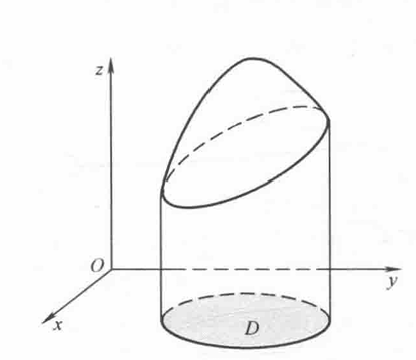
\includegraphics[width=0.5\textwidth]{Neighborhood_of_a multivariable_function.png}
\end{center}

和一元函数一样，我们首先要有\textbf{邻域}的概念。对于点 $P_0(x_0,y_0)$ 的 $\delta$ 邻域，就是以它为中心的一个小圆盘，定义为
\[
U_\delta(P_0)=\{(x,y)\mid \sqrt{(x-x_0)^2+(y-y_0)^2}<\delta\}.
\]

于是\textbf{二元函数极限}就可以描述为：若存在常数 $A$，使得对任意 $\varepsilon>0$，存在 $\delta>0$，当
$(x,y)\in \dot U_\delta(P_0)$ 时都有
\[
|f(x,y)-A|<\varepsilon,
\]

\[
\lim_{(x,y)\to(x_0,y_0)}f(x,y)=A.
\]

你会发现，这和一元函数的定义在精神上几乎一模一样，只不过“左右逼近”变成了“从平面里所有方向逼近”。真正增加的不是公式复杂度，而是逼近方式的自由度。

\textbf{连续性}的定义也仍然是同一套语言：若
\[
\lim_{(x,y)\to(x_0,y_0)}f(x,y)=f(x_0,y_0),
\]
则称 $f$ 在点 $(x_0,y_0)$ 连续。

但是一进入多元函数，很多你在一元世界里形成的习惯就需要重新审视。比如一元函数里我们知道可导一定连续，而多元函数里要判断可微，却不能只看某一个方向。因为平面不只有左右两个方向，而是有无穷多个方向，所以你要想描述这个曲面的变化率，最自然的第一步，就是先沿着两条坐标方向分别去看它怎样变化。这就是偏导数的出发点。数学上，偏导数的定义直接仿照一元函数写成：
\[
\frac{\partial f}{\partial x}(x_0,y_0)
=\lim_{\Delta x\to 0}\frac{f(x_0+\Delta x,y_0)-f(x_0,y_0)}{\Delta x}.
\]
\[
\frac{\partial f}{\partial y}(x_0,y_0)
=\lim_{\Delta y\to 0}\frac{f(x_0,y_0+\Delta y)-f(x_0,y_0)}{\Delta y}.
\]

它的\textbf{几何意义}也很好理解。比如
$\frac{\partial f}{\partial x}(x_0,y_0)$ 表示曲面 $z=f(x,y)$ 在点
$(x_0,y_0,f(x_0,y_0))$ 处，沿 $x$ 方向截线的切线斜率；
$\frac{\partial f}{\partial y}(x_0,y_0)$ 类似地表示沿 $y$ 方向的切线斜率。也就是说，偏导数并没有一下子告诉你整个曲面怎样弯，而只是先告诉你：如果我只沿着某一条最基本的方向去走，会看到什么。

\subsection{复合函数求导和雅可比矩阵}

在多元函数中，链式法则可以理解为“外层变化率乘以内层变化率，再把所有可能路径的贡献加起来”。我们设
\[
z=f(u,v),\qquad u=u(x,y),\ v=v(x,y),
\]
且各函数在对应点可微，则复合函数 $z=z(x,y)$ 的偏导为
\[
\frac{\partial z}{\partial x}=\frac{\partial f}{\partial u}\frac{\partial u}{\partial x}
+\frac{\partial f}{\partial v}\frac{\partial v}{\partial x},
\qquad
\frac{\partial z}{\partial y}=\frac{\partial f}{\partial u}\frac{\partial u}{\partial y}
+\frac{\partial f}{\partial v}\frac{\partial v}{\partial y}.
\]

这看起来像简单套公式，但真正值得记住的是：在多元世界里，一个变量的变化常常会通过不止一条路径传导到最终结果上，因此总变化率是“所有路径贡献的总和”。

更复杂的情况是隐函数。比如你只知道一个关系式
\[
f(x,y)=0,
\]
但你真正想求的是 $y$ 关于 $x$ 的导数，而函数又不是显式写成 $y=f(x)$ 的形式。这时我们就沿用一元微积分的想法，把整个关系一起求导：
\[
\frac{\partial f}{\partial x}+\frac{\partial f}{\partial y}\frac{dy}{dx}=0,
\]
无论几元函数，最后的结果一定是这个样子的，因为\textbf{自变量之间是绝对独立的}，也就是说自变量在偏导的时候互为常数，但是全导不是，我知道你们一定看不懂我雄鹰般的语言系统，举个例子：对于三元函数$u(x,y,z)$求$z$对$x$的导数怎么办？我们依旧直接让$z$对$x$求全导就好了，这时候$y$还是被视为常数。

但是如果给出更多的约束条件那么情况就大有所不同了,这时候 $x$,$y$,$z$ 就不再是独立的自变量了，它们构成了一个约束曲面。例如考虑二元方程组：
\[
\begin{cases}
F(x,y,u,v)=0,\\
G(x,y,u,v)=0,
\end{cases}
\]
这是一个典型的二元隐函数系统（把 $u,v$ 视作关于 $x,y$ 的隐函数）。我们对整体求导，会得到一个关于未知偏导数的线性系统，对于二维系统而言直接求解结构了，但是对于更高维的方程组我们人类无法轻易求解，而想到线性系统的解天然会和行列式联系起来，于是雅可比行列式便出现了。
\[
J=\frac{\partial(F,G)}{\partial(u,v)}
=\begin{vmatrix}
F_u & F_v\\
G_u & G_v
\end{vmatrix}\neq 0,
\]
则由隐函数定理可知局部可解为 $u=u(x,y),\ v=v(x,y)$，并且
\[
\frac{\partial u}{\partial x}
=-\frac{\dfrac{\partial(F,G)}{\partial(x,v)}}{\dfrac{\partial(F,G)}{\partial(u,v)}},
\qquad
\frac{\partial v}{\partial x}
=-\frac{\dfrac{\partial(F,G)}{\partial(u,x)}}{\dfrac{\partial(F,G)}{\partial(u,v)}},
\]
\[
\frac{\partial u}{\partial y}
=-\frac{\dfrac{\partial(F,G)}{\partial(y,v)}}{\dfrac{\partial(F,G)}{\partial(u,v)}},
\qquad
\frac{\partial v}{\partial y}
=-\frac{\dfrac{\partial(F,G)}{\partial(u,y)}}{\dfrac{\partial(F,G)}{\partial(u,v)}}.
\]

这就是“用雅可比行列式写解”的标准形式。推而广之，$n$ 元方程组的雅可比矩阵也是类似的。这里 $J_{\mathbf{g}}$ 称为 $\mathbf{g}$ 的\textbf{雅可比矩阵}，定义为
\[
J_{\mathbf{g}}(\mathbf{x})=
\begin{bmatrix}
\dfrac{\partial g_1}{\partial x_1} & \cdots & \dfrac{\partial g_1}{\partial x_n}\\
\vdots & \ddots & \vdots\\
\dfrac{\partial g_m}{\partial x_1} & \cdots & \dfrac{\partial g_m}{\partial x_n}
\end{bmatrix}.
\]

当 $m=n$ 时，其行列式
\[
\dfrac{\partial(g_1,\dots,g_n)}{\partial(x_1,\dots,x_n)}=\det J_{\mathbf{g}}(\mathbf{x})
\]
它记录的，其实就是这个变换在局部把空间怎样拉伸、压缩或翻转。

\subsection{全微分的定义与成立条件到方向导数}

接下来我们继续讨论二元函数的微元。既然已经有了偏导，自然就会有两个最基本方向上的线性变化：
\[
\frac{\partial f}{\partial x}dx\qquad\frac{\partial f}{\partial y}dy
\]
但问题也立刻显现出来：这还只是沿坐标方向各自的变化，它们还没有告诉你函数在平面里任意微小位移下到底总共改变了多少。于是为了真正描述整体变化，我们先写出全增量。设 $z=f(x,y)$，在点 $(x_0,y_0)$ 的增量为
\[
\Delta z=f(x_0+\Delta x,y_0+\Delta y)-f(x_0,y_0).
\]

现在的问题是：怎样把一个我们根本不知道具体表达式的函数增量，拆成“线性主部 + 更高阶小量”？这时只能借助一元微积分里的中值定理，把二维变化拆成两步走。于是先凑项：
\[
\begin{aligned}
\Delta z
&=\bigl[f(x_0+\Delta x,y_0+\Delta y)-f(x_0,y_0+\Delta y)\bigr]
+\bigl[f(x_0,y_0+\Delta y)-f(x_0,y_0)\bigr].
\end{aligned}
\]
对第一项把 $y=y_0+\Delta y$ 视为常数，关于 $x$ 用一元中值定理，存在
$\theta_1\in(0,1)$ 使
\[
f(x_0+\Delta x,y_0+\Delta y)-f(x_0,y_0+\Delta y)
=\frac{\partial f}{\partial x}(x_0+\theta_1\Delta x,\,y_0+\Delta y)\,\Delta x.
\]
对第二项把 $x=x_0$ 视为常数，关于 $y$ 用一元中值定理，存在
$\theta_2\in(0,1)$ 使
\[
f(x_0,y_0+\Delta y)-f(x_0,y_0)
=\frac{\partial f}{\partial y}(x_0,\,y_0+\theta_2\Delta y)\,\Delta y.
\]
因此
\[
\Delta z=\frac{\partial f}{\partial x}(x_0+\theta_1\Delta x,\,y_0+\Delta y)\,\Delta x
+\frac{\partial f}{\partial y}(x_0,\,y_0+\theta_2\Delta y)\,\Delta y.
\]
若两个偏导数在 $(x_0,y_0)$ 连续，那么上式右边的两个偏导值都会分别趋向
$\dfrac{\partial f}{\partial x}(x_0,y_0)$ 与 $\dfrac{\partial f}{\partial y}(x_0,y_0)$。于是我们把它们和基点处的偏导数作差，记
\[
\eta_1=\frac{\partial f}{\partial x}(x_0+\theta_1\Delta x,\,y_0+\Delta y)-\frac{\partial f}{\partial x}(x_0,y_0),
\]
\[
\eta_2=\frac{\partial f}{\partial y}(x_0,\,y_0+\theta_2\Delta y)-\frac{\partial f}{\partial y}(x_0,y_0).
\]
那么当 $(\Delta x,\Delta y)\to(0,0)$ 时，$\eta_1\to0$，$\eta_2\to0$，并且
\[
\Delta z=\frac{\partial f}{\partial x}(x_0,y_0)\Delta x+\frac{\partial f}{\partial y}(x_0,y_0)\Delta y+\eta_1\Delta x+\eta_2\Delta y.
\]

现在真正要解释的是：为什么最后那两项确实比一阶主部更小？因为
\[
|\eta_1\Delta x+\eta_2\Delta y|
\le |\eta_1|\,|\Delta x|+|\eta_2|\,|\Delta y|
\le (|\eta_1|+|\eta_2|)\sqrt{(\Delta x)^2+(\Delta y)^2}.
\]
而 $|\eta_1|+|\eta_2|\to0$，所以这整个余项相对于邻域半径
$\sqrt{(\Delta x)^2+(\Delta y)^2}$ 来说，确实是更高阶的小量。也就是说，真正主导函数变化的，是那两个一阶线性项；其余部分在尺度缩小时会更快消失。这也解释了为什么“偏导连续”常常足以推出“函数可微”：它保证了这种线性近似不是偶然碰巧，而是在各个方向上都稳定成立。

于是余项满足
\[
  \eta_1\Delta x+\eta_2\Delta y=o\!\left(\sqrt{(\Delta x)^2+(\Delta y)^2}\right)
  \quad ((\Delta x,\Delta y)\to(0,0)).
\]
因此我们就可以把 $\Delta z$ 写成

\[
\Delta z=\frac{\partial f}{\partial x}(x_0,y_0)\Delta x+\frac{\partial f}{\partial y}(x_0,y_0)\Delta y+o\!\left(\sqrt{(\Delta x)^2+(\Delta y)^2}\right)
\quad((\Delta x,\Delta y)\to(0,0)),
\]
则称 $f$ 在 $(x_0,y_0)$ \textbf{可微}，并称
\[
\mathrm{d}z=\frac{\partial f}{\partial x}(x_0,y_0)\mathrm{d}x+\frac{\partial f}{\partial y}(x_0,y_0)\mathrm{d}y.
\]
为该点的\textbf{全微分}。

从上述讨论我们不难看出：
\begin{itemize}
  \item \textbf{可微的必要性}是偏导数 $f'_x,f'_y$ 在该点存在。这时候你至少能写出候选的线性主部。
  \item \textbf{可微的充分性}是 $f'_x,f'_y$ 在 $(x_0,y_0)$ 的某邻域内存在且在该点连续。这样线性近似不只是形式上存在，而且真的能稳定控制误差。
\end{itemize}

在物理学中常用的全微分展开，就是建立在这个定义上的。若函数在该点邻域内有足够光滑的高阶偏导数，那么还可以继续写出二阶泰勒展开：
\[
\begin{aligned}
f(x_0+\Delta x,y_0+\Delta y)
={}&f(x_0,y_0)+\partial_x f(x_0,y_0)\Delta x+\partial_y f(x_0,y_0)\Delta y\\
&+\frac12\bigl(\partial_{xx}f(x_0,y_0)\Delta x^2+2\partial_{xy}f(x_0,y_0)\Delta x\Delta y+\partial_{yy}f(x_0,y_0)\Delta y^2\bigr)\\
&+o\!\left((\Delta x^2+\Delta y^2)^{\frac32}\right).
\end{aligned}
\]
这里的 $o\!\left((\Delta x^2+\Delta y^2)^{\frac32}\right)$ 表示三次小量；若只保留线性主部，则退化回前面的全微分近似。也就是说，泰勒展开只是把“局部近似”这件事从一阶继续向更高阶推进。


不难发现，全微分的一般形式都是形似：
\[
dz=Pdx+Qdy
\]
但是这并不意味着所有长成这个样子的微分都是全微分，要判断一个这样的微分式到底是不是一个全微分，需要用到的判据叫做“曲线积分是否和路径无关”，那很显然了这个事情肯定和曲线积分有着莫大的联系，大家可以先去第\pageref{path-independent}页看看曲线积分是怎么回事，特别是格林公式。总而言之，我们考虑 $Pdx+Qdy$ 为某个函数 $F(x,y)$ 的全微分，那么一定有
\[
P=\frac{\partial F}{\partial x},\qquad Q=\frac{\partial F}{\partial y}.
\]

任取区域内两点 $A$、$B$，以及连接 $A$、$B$ 的任意一条光滑曲线 $C$，其参数方程为
\[
x=x(t),\qquad y=y(t),\qquad \alpha\leq t\leq \beta,
\]
其中 $A=(x(\alpha),y(\alpha))$，$B=(x(\beta),y(\beta))$，沿曲线 $C$ 计算积分，由链式法则，沿曲线 $C$ 有
\[
\int_C Pdx+Qdy
=\int_C \frac{\partial F}{\partial x}dx+\frac{\partial F}{\partial y}dy
=dF(x(t),y(t))
=\int_\alpha^\beta \frac{dF}{dt}\,dt
=F(B)-F(A).
\]

上式右端仅与起点 $A$ 和终点 $B$ 有关，而与路径 $C$ 的具体选择无关。因此，对于连接 $A$、$B$ 的任意两条路径 $C_1$、$C_2$，都有
\[
\int_{C_1} Pdx+Qdy=F(B)-F(A)=\int_{C_2} Pdx+Qdy.
\]
故曲线积分与路径无关。必要性得证。

现在我们来考虑充分性，也是我们这部分的主要判据。若曲线积分与路径无关，则对区域内任意一条闭曲线 $C$，有
\[
\oint_C Pdx+Qdy=0.
\]
这描述了一个封闭回路所有全微分的积分沿着路径走一圈是$0$，很显然这就是微分的基本性质。由格林公式，
\[
\oint_C Pdx+Qdy
=\iint_D \left(\frac{\partial Q}{\partial x}-\frac{\partial P}{\partial y}\right)\,dxdy.
\]

因此必有
\[
\frac{\partial P}{\partial y}=\frac{\partial Q}{\partial x}
\]
在 $D$ 内处处成立。而上式正是 $Pdx+Qdy$ 为全微分的充要条件，故充分性得证。

不过这就远远偏离我们最初的想法了，回到我们最初的想法：如何求任意方向的导数\label{directional_derivative}？既然我们已经知道全增量满足
\[
f(x_0+\Delta x,y_0+\Delta y)-f(x_0,y_0)
=\frac{\partial f}{\partial x}(x_0,y_0)\Delta x+\frac{\partial f}{\partial y}(x_0,y_0)\Delta y +o\!\left(\sqrt{(\Delta x)^2+(\Delta y)^2}\right)
.
\]
那么只要把这个式子的每一项都除以位移长度 $\sqrt{(\Delta x)^2+(\Delta y)^2}$，方向导数的轮廓就已经出来了：
\[
\frac{f(x_0+\Delta x,y_0+\Delta y)-f(x_0,y_0)}{\sqrt{(\Delta x)^2+(\Delta y)^2}}
=\frac{\partial f}{\partial x}(x_0,y_0)\frac{\Delta x}{\sqrt{(\Delta x)^2+(\Delta y)^2}}
+\frac{\partial f}{\partial y}(x_0,y_0)\frac{\Delta y}{\sqrt{(\Delta x)^2+(\Delta y)^2}}
+o.
\]
若位移方向固定为单位向量 $\mathbf u=(\cos\theta,\sin\theta)$，那么
\[
\frac{\Delta x}{\sqrt{(\Delta x)^2+(\Delta y)^2}}\to \cos\theta,
\qquad
\frac{\Delta y}{\sqrt{(\Delta x)^2+(\Delta y)^2}}\to \sin\theta.
\]
于是方向导数自然写成
\[
 D_{\mathbf{u}}f=\frac{f(x_0+\Delta x,y_0+\Delta y)-f(x_0,y_0)}{\sqrt{(\Delta x)^2+(\Delta y)^2}}
=\frac{\partial f}{\partial x}(x_0,y_0)\cos\theta
+\frac{\partial f}{\partial y}(x_0,y_0)\sin\theta.
\]
这里的三角函数并不神秘，它们就是单位方向向量在二维坐标轴上的分量。于是要说明方向导数 $D_{\mathbf{u}}f$ 何时取得最大值，我们自然会想到点积。于是我们定义梯度向量
\[\nabla f = \left( \frac{\partial f}{\partial x}, \frac{\partial f}{\partial y} \right)
\]
加上单位方向向量 $\mathbf{u} = (\cos\theta, \sin\theta)$，则方向导数可表示为
\[
        D_{\mathbf{u}}f = \nabla f \cdot \mathbf{u} = \|\nabla f\| \|\mathbf{u}\| \cos\alpha
\]
其中 $\|\nabla f\|$ 是梯度模长，$\|\mathbf{u}\|=1$ 是单位向量模长，$\alpha$ 是向量 $\nabla f$ 与 $\mathbf{u}$ 之间的夹角。
由于 $\|\nabla f\|$ 在给定点处为常数，欲使 $D_{\mathbf{u}}f$ 最大，只需使 $\cos\alpha$ 最大。
当 $\alpha = 0$ 时，$\cos\alpha = 1$，此时 $D_{\mathbf{u}}f$ 取得最大值 $\|\nabla f\|$。
$\alpha = 0$ 意味着单位向量 $\mathbf{u}$ 的方向与梯度向量 $\nabla f$ 的方向完全相同。
   
综上所述，函数在某一点的增长最快方向即为梯度方向，其最大增长率为梯度的模长 $\|\nabla f\|$。

\subsection{梯度、极值与多元积分}

学到这里，我们其实已经隐约看见了一件很重要的事：偏导数虽然有用，但它太零碎了。它一次只告诉你沿某一个坐标轴方向怎样变化，可真实的问题很少只沿着 $x$ 轴或者 $y$ 轴发生。你真正想知道的是：在空间里的某一点，这个量到底朝哪里变化得最快，哪里根本不变，哪里像在往外冒，哪里又像在原地打转。于是人们开始想，要是能把这些分散的偏导数重新组织起来，像把一堆零件装成一台机器那样，能不能一下子看出整个场的局部结构？这就是向量分析诞生时最自然的动机。

首先出场的是梯度。我们把
\[
\nabla=\left(\frac{\partial}{\partial x},\frac{\partial}{\partial y},\frac{\partial}{\partial z}\right)
\]
看成一个“会微分的向量”。它本身不是普通向量，而更像一个等待作用的算符。它一旦作用在标量场 $\phi=\phi(x,y,z)$ 上，就得到
\[
\nabla\phi=
\left(\frac{\partial \phi}{\partial x},\frac{\partial \phi}{\partial y},\frac{\partial \phi}{\partial z}\right).
\]
这不是为了写法好看才这么定义的，而是因为它恰好把“各个方向上的变化率”打包成了一个几何对象。前面我们已经看到，方向导数可以写成 $D_{\mathbf u}\phi=\nabla\phi\cdot\mathbf u$，于是梯度的方向就是函数增长最快的方向，而它的模长就是最大方向导数。换句话说，当你站在一座山的某一点，梯度指向的就是最陡的上坡方向；若梯度为零，那就说明你在局部已经感觉不到一阶上的“上坡”或“下坡”了。

但自然界里不只有标量场。温度、势能这类量在每一点只给出一个数，可速度场、电场、力场在每一点给出的是一个向量。于是新的问题来了：一个向量场到底在说什么？设
\[
\mathbf{F}=(P,Q,R),
\]
我们可以把它想成一团充满空间的小箭头。现在不要急着算公式，先问一个更直观的问题：如果我在某一点周围取一个极小的小球，这些箭头总体上是更倾向于从里面流出去，还是从外面流进来？描述这件事的量就是散度：
\[
\nabla\cdot\mathbf{F}=\frac{\partial P}{\partial x}+\frac{\partial Q}{\partial y}+\frac{\partial R}{\partial z}.
\]
若它大于零，这个点附近更像一个源，仿佛有什么东西从里面涌出；若它小于零，这里更像一个汇，仿佛有什么东西被吸进去；若它等于零，就表示局部没有净流出也没有净流入。在流体力学里，不可压缩流体就常常满足这样的条件。这个定义看起来只是三个偏导数相加，但真正值得记住的是它背后的图像：散度测量的不是箭头有多大，而是“有没有净产生”这件事。

可空间中的箭头还有另一种可能：它们并不向外冒，也不向里缩，而是在一个点附近绕着打转。你把一小片树叶扔进水里，树叶会不会开始旋转？这时我们需要的不是散度，而是旋度。对向量场 $\mathbf{F}=(P,Q,R)$，定义
\[
\nabla\times\mathbf{F}=
\left(
\frac{\partial R}{\partial y}-\frac{\partial Q}{\partial z},
\frac{\partial P}{\partial z}-\frac{\partial R}{\partial x},
\frac{\partial Q}{\partial x}-\frac{\partial P}{\partial y}
\right),
\]
也可以记成行列式形式
\[
\nabla\times\mathbf{F}=
\begin{vmatrix}
\mathbf{i}&\mathbf{j}&\mathbf{k}\\
\dfrac{\partial}{\partial x}&\dfrac{\partial}{\partial y}&\dfrac{\partial}{\partial z}\\
P&Q&R
\end{vmatrix}.
\]
它刻画的是局部的旋转趋势。若 $\nabla\times\mathbf{F}=\mathbf{0}$，我们就说这个场在该区域无旋。你可以把散度和旋度看成两种完全不同的“局部检查”：前者问的是有没有净流出，后者问的是有没有局部打转。一个场可以无旋但有散度，也可以有旋但无散度，这两件事千万别混在一起。

然后还有一个在数学和物理里频繁出现的角色：拉普拉斯算符。它可以看成“先取梯度，再取散度”，于是对标量场 $\phi$ 有
\[
\Delta\phi=\nabla\cdot\nabla\phi
=\frac{\partial^2\phi}{\partial x^2}
+\frac{\partial^2\phi}{\partial y^2}
+\frac{\partial^2\phi}{\partial z^2}.
\]
这个式子看起来朴素得几乎不像一个重要对象，但它几乎无处不在：热会如何扩散，弦会如何振动，引力势和电势如何由源分布决定，这些问题最后都会碰到它。若 $\Delta\phi=0$，则 $\phi$ 称为调和函数。它们有一种很特别的平衡感：在局部没有额外的“鼓起”或“凹下”，像一张被自然拉平的薄膜。

一旦接受了 $\nabla$ 是个统一的微分机器，很多公式就不再像零散技巧，而像同一台机器吐出的不同结果。例如
\[
\nabla\cdot(\nabla\times\mathbf{F})=0,
\qquad
\nabla\times(\nabla\phi)=\mathbf{0}.
\]
这两条公式值得反复咀嚼：由纯旋转构成的东西不可能凭空制造源汇，而由纯粹“爬坡”得到的场也不可能自发形成环流。再比如乘法法则
\[
\nabla\cdot(\phi\mathbf{F})=\nabla\phi\cdot\mathbf{F}+\phi\,\nabla\cdot\mathbf{F},
\]
\[
\nabla\times(\phi\mathbf{F})=\nabla\phi\times\mathbf{F}+\phi\,(\nabla\times\mathbf{F}),
\]
以及二阶恒等式
\[
\nabla\times(\nabla\times\mathbf{F})
=\nabla(\nabla\cdot\mathbf{F})-\Delta\mathbf{F},
\qquad
\Delta\mathbf{F}=(\Delta P,\Delta Q,\Delta R).
\]
它们真正的价值不在于背下来，而在于你逐渐会发现：很多看起来复杂的场论表达式，只是在这些基本结构之间来回变形而已。数学训练做到后面，往往不是公式更多，而是你终于认出了公式背后的骨架。

现在我们把目光从“场怎样变化”转向“函数在哪里取极值”。一元函数里，极大极小通常出现在导数为零或导数不存在的地方。多元函数并没有改变这个逻辑，只是把“导数”换成了梯度。设 $z=f(x,y)$，若 $(x_0,y_0)$ 是定义域内部点，且 $f$ 在该点可微，那么如果 $f$ 在这里取得局部极大值或局部极小值，就必须满足
\[
f_x(x_0,y_0)=0,\qquad f_y(x_0,y_0)=0,
\]
也就是
\[
\nabla f(x_0,y_0)=\mathbf{0}.
\]
这样的点叫做驻点。可你千万别把“驻点”误听成“极值点”，因为函数有时只是暂时停住，却并没有真的到达山顶或谷底。最经典的例子是
\[
f(x,y)=x^2-y^2.
\]
在原点处，两个一阶偏导都为零，但如果沿着 $x$ 轴走，你觉得它像个谷底；沿着 $y$ 轴走，你又觉得它像个山顶。于是原点两头都像，却哪头都不是，它是一匹马鞍的鞍部，所以叫鞍点。这个例子非常重要，因为它提醒我们：一阶信息只能告诉你“这里暂时平了”，却不能告诉你“这里到底是顶、底，还是拐过去的地方”。

那么接下来该看什么？当然是二阶变化。对二元函数，若在 $(x_0,y_0)$ 的邻域内二阶偏导连续，记
\[
A=f_{xx}(x_0,y_0),\qquad B=f_{xy}(x_0,y_0),\qquad C=f_{yy}(x_0,y_0),
\]
并构造判别式
\[
D=AC-B^2.
\]
它的判定规则是
\[
\begin{cases}
D>0,\ A>0,&\text{局部极小值},\\
D>0,\ A<0,&\text{局部极大值},\\
D<0,&\text{鞍点}.
\end{cases}
\]
若 $D=0$，这套判据就暂时失灵，还得往更高阶看。这个规则看起来像考试技巧，其实本质非常几何：二阶项决定了函数在该点附近最先显露出来的曲面形状。它到底像一只碗、像一只倒扣的碗，还是像马鞍，取决于那个二次型的符号性质。到了高维，事情的语言会变得更整齐。设
\[
f=f(x_1,x_2,\dots,x_n),
\]
当 $\nabla f(\mathbf{x}_0)=\mathbf{0}$ 时，我们考察 Hessian 矩阵
\[
H_f(\mathbf{x}_0) = \begin{pmatrix}
\frac{\partial^2 f}{\partial x_1^2}(\mathbf{x}_0) & \frac{\partial^2 f}{\partial x_1 \partial x_2}(\mathbf{x}_0) & \cdots & \frac{\partial^2 f}{\partial x_1 \partial x_n}(\mathbf{x}_0) \\[6pt]
\frac{\partial^2 f}{\partial x_2 \partial x_1}(\mathbf{x}_0) & \frac{\partial^2 f}{\partial x_2^2}(\mathbf{x}_0) & \cdots & \frac{\partial^2 f}{\partial x_2 \partial x_n}(\mathbf{x}_0) \\[6pt]
\vdots & \vdots & \ddots & \vdots \\[6pt]
\frac{\partial^2 f}{\partial x_n \partial x_1}(\mathbf{x}_0) & \frac{\partial^2 f}{\partial x_n \partial x_2}(\mathbf{x}_0) & \cdots & \frac{\partial^2 f}{\partial x_n^2}(\mathbf{x}_0)
\end{pmatrix}_{n \times n}.
\]
若它正定，则 $\mathbf{x}_0$ 为局部极小点；若它负定，则为局部极大点；若它不定，则为鞍点。你会发现，所谓极值判定，本质上就是在研究“局部二次近似”的正负性。函数在足够小的尺度下，看起来越来越像一个二次型，而我们判断的正是这个近似模型的性格。

不过真正有趣的问题常常带着约束。你不是在整个平面上找最大最小，而是在一条曲线上、一个曲面上，或者某种守恒条件下去找。这时只令 $f_x=f_y=0$ 就不对了，因为你根本没有资格朝所有方向走；你只能沿着约束允许的方向移动。设约束为
\[
g(x,y)=0,
\]
那么在约束曲线上求极值时，常用拉格朗日乘子法：
\[
\nabla f(x,y)=\lambda\,\nabla g(x,y),\qquad g(x,y)=0.
\]
这行公式之所以漂亮，不是因为它多了个新字母 $\lambda$，而是因为它把几何直觉翻译成了代数语言。在极值点上，目标函数的等值线与约束曲线相切，所以它们的法向量必定平行。也就是说，真正的限制不是“梯度为零”，而是“梯度不能再沿约束方向产生一阶变化”。

\begin{center}
  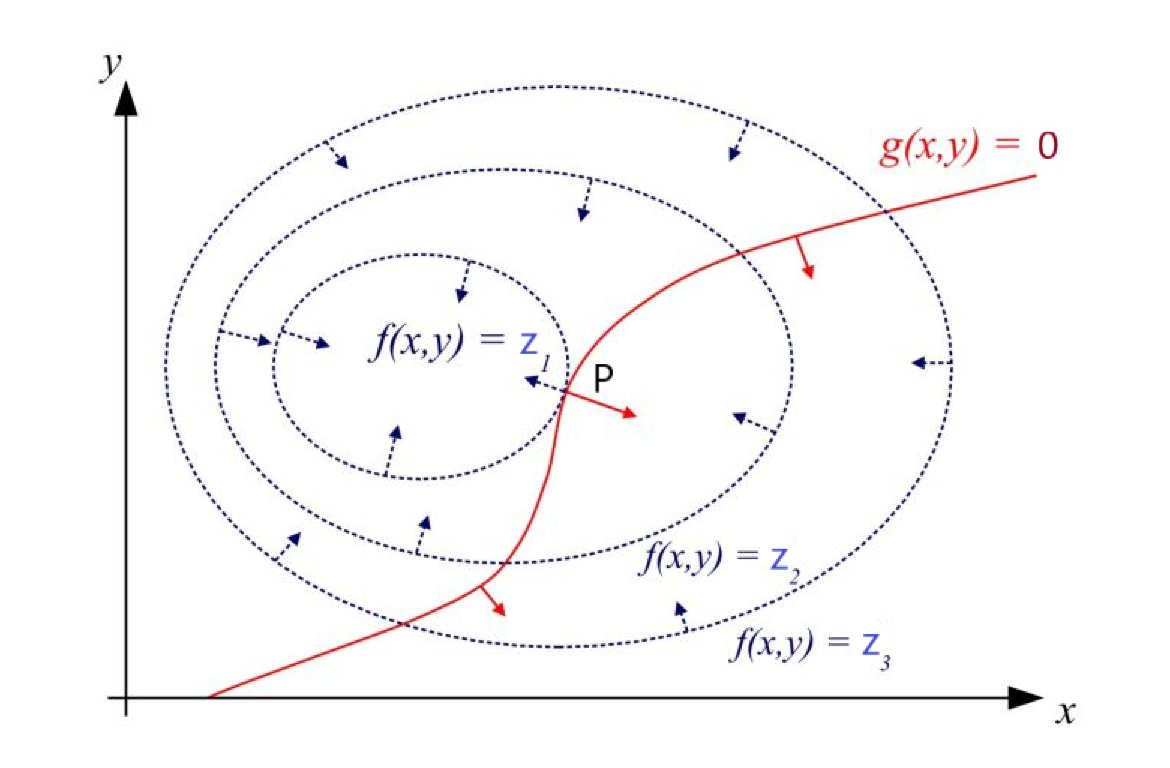
\includegraphics[width=0.5\textwidth]{image.png}
\end{center}

设约束曲线 $g(x,y)=0$ 上有一条参数曲线 $\mathbf{r}(t)=(x(t),y(t))$，且对任意 $t$ 都有 $g(x(t),y(t))=0$。我们要在曲线上求 $f$ 的极值，考虑
\[
F(t)=f(x(t),y(t)).
\]
若在曲线上某点取得局部极值，则必有 $F'(t)=0$。由链式法则，
\[
F'(t)=\nabla f\cdot\mathbf{r}'(t)=0.
\]
而由 $g(x(t),y(t))=0$ 对 $t$ 求导，得到
\[
\nabla g\cdot\mathbf{r}'(t)=0.
\]
这说明切向量 $\mathbf{r}'(t)$ 同时与 $\nabla f$ 和 $\nabla g$ 正交。在二维平面中，与同一非零切向量正交的所有向量都落在同一条直线上，因此 $\nabla f$ 与 $\nabla g$ 必然共线，即存在 $\lambda$ 使得
\[
\nabla f=\lambda\,\nabla g.
\]
这就是拉格朗日乘子法的具体原理，是不是很有趣？本质上就是对梯度的一个简单应用，在这里因为是二维平面所以 $\nabla f$ 与 $\nabla g$ 必然共线，但是在更高维度的空间就不是这样了，我们考虑$\mathbb{R}^n$ 上的函数 $f$  ，有 $m$ 个约束（$m<n$）：
\[
g_1(\mathbf{x})=0,\; g_2(\mathbf{x})=0,\; \dots,\; g_m(\mathbf{x})=0.
\]
这些方程定义了一个 $n-m$ 维的约束曲面。假设各 $\nabla g_i$ 线性无关，则约束曲面上过任意点的切空间恰好是所有 $\nabla g_i$ 的正交补。

极值条件仍然是：$f$ 沿切空间内任何方向的方向导数都为零。这意味着 $\nabla f$ 与整个切空间正交，因此 $\nabla f$ 必须落在由所有 $\nabla g_i$ 张成的子空间里。于是存在乘子 $\lambda_1,\lambda_2,\dots,\lambda_m$，使得
\[
\nabla f=\lambda_1\nabla g_1+\lambda_2\nabla g_2+\cdots+\lambda_m\nabla g_m.
\]

定义拉格朗日函数
\[
\mathcal{L}(\mathbf{x},\boldsymbol{\lambda})=f(\mathbf{x})-\sum_{i=1}^m\lambda_i g_i(\mathbf{x}),
\]
对 $\mathbf{x}$ 求梯度并令其为零即得上述方程，对 $\lambda_i$ 求导则得约束方程 $g_i(\mathbf{x})=0$。

整个方法的核心始终是“在切空间上没有一阶变化”，代数形式只是这一几何事实的等价表达。若约束不是光滑的，或极值点处 $\nabla g_i$ 线性相关，则上述推导的前提不成立。

\newpage

\section{多元函数积分}

最后我们来到多元函数积分。若说导数研究的是局部怎样变化，那么积分研究的就是这些局部变化怎样累积成总体。在一元函数里，积分常被解释为曲线下的面积；到了二元函数 $z=f(x,y)$，我们面对的不再是一条区间，而是一整块平面区域。最自然的想法是：把区域 $D$ 切成许多很小的小块，每一块面积记作 $\Delta\sigma_k$，在第 $k$ 块里任选一点 $(\xi_k,\eta_k)$，那么这一小块贡献的总量近似是
\[
f(\xi_k,\eta_k)\,\Delta\sigma_k.
\]
把所有小块加起来，就得到
\[
\sum_{k=1}^n f(\xi_k,\eta_k)\,\Delta\sigma_k.
\]
当分割越来越细、每一小块的直径都趋于零时，如果这个和有极限，我们就把它定义为二重积分：
\[
\iint_D f(x,y)\,\mathrm{d}\sigma.
\]
这里的 $\mathrm{d}\sigma$ 或 $\mathrm{d}A$ 就是面积微元。它听起来抽象，其实意思非常朴素：那只是“无限小的一块面积”。如果 $f(x,y)\equiv 1$，那么每一小块只是在单纯地数面积，于是
\[
\iint_D 1\,\mathrm{d}A=\mathrm{Area}(D).
\]
所以一般二重积分可以看作带权面积，或者更广泛地说，是平面区域上的总体累积。

\subsection{二重积分}

真正开始计算时，关键不在积分号本身，而在你怎样切这块区域。在直角坐标系中，最自然的面积微元是小矩形，于是
\[
\mathrm{d}A=\mathrm{d}x\,\mathrm{d}y.
\]
若区域写成
\[
D=\{(x,y)\mid a\le x\le b,\ y_1(x)\le y\le y_2(x)\},
\]
那么二重积分就能改写为
\[
\iint_D f(x,y)\,\mathrm{d}A
=\int_a^b\!\left(\int_{y_1(x)}^{y_2(x)} f(x,y)\,\mathrm{d}y\right)\mathrm{d}x.
\]
\begin{center}
  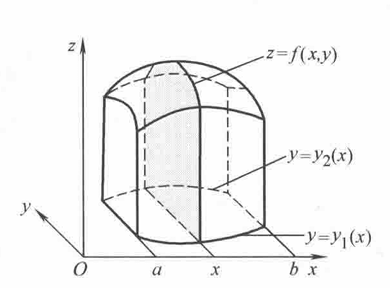
\includegraphics{2.6-1.png}
\end{center}

这句话的意思并不神秘：先固定 $x$，沿竖直方向把一条小线段上的贡献加起来，再让这条线段从左到右扫过整个区域。若区域更适合写成
\[
D=\{(x,y)\mid c\le y\le d,\ x_1(y)\le x\le x_2(y)\},
\]
那么也可以反过来先对 $x$ 积：
\[
\iint_D f(x,y)\,\mathrm{d}A
=\int_c^d\!\left(\int_{x_1(y)}^{x_2(y)} f(x,y)\,\mathrm{d}x\right)\mathrm{d}y.
\]

所以二重积分里最需要训练的直觉不是“会不会积分”，而是“会不会看区域”。图一旦画清楚，先积谁、后积谁，往往就顺了。



不过坐标并不是神圣不可改变的。若区域长得像圆、扇形、圆环，硬用直角坐标会把问题写得很别扭，这时极坐标就像专门为它们定做的一样。令
\[
x=r\cos\theta,\qquad y=r\sin\theta,
\]
你也许会想，面积微元是不是就简单变成 $\mathrm{d}r\,\mathrm{d}\theta$？这里恰恰有一个必须真正理解的细节：不是。因为在极坐标下，一个很小的小块并不是“小长方形”，而更像一块极细的扇环，它的面积约等于“半径方向厚度 $\mathrm{d}r$”乘上“圆弧长度 $r\,\mathrm{d}\theta$”，所以
\[
\mathrm{d}A=r\,\mathrm{d}r\,\mathrm{d}\theta.
\]
\begin{center}
  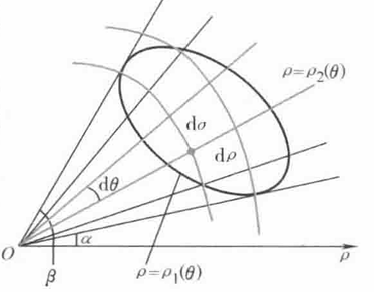
\includegraphics{2.6-2.png}
\end{center}

这个额外的 $r$ 绝不是装饰品，它反映的是同样大小的角度在远离原点时会扫出更长的弧。于是若区域在极坐标下表示为
\[
D=\{(r,\theta)\mid \alpha\le \theta\le \beta,\ r_1(\theta)\le r\le r_2(\theta)\},
\]
那么
\[
\iint_D f(x,y)\,\mathrm{d}A
=\int_{\alpha}^{\beta}\!\left(\int_{r_1(\theta)}^{r_2(\theta)} f(r\cos\theta,r\sin\theta)\,r\,\mathrm{d}r\right)\mathrm{d}\theta.
\]
做这种积分时，真正要同时记住三件事：区域边界要改写成 $r,\theta$ 的范围，被积函数里的 $x,y$ 要换成 $r\cos\theta,r\sin\theta$，而面积微元里那个 $r$ 一定不能丢。很多计算错误其实都不是算错，而是在变量代换的那一刻，没有真的接受“坐标变了，几何单位也跟着变了”这件事。

从形式上而言，我们经常会对这样一个积分形式感到熟悉而又神秘：
\[
 \iint_D \frac{x f'_x + y f'_y}{x^2 + y^2} \, \mathrm{d}x\mathrm{d}y 
\]
它看起来既像是一个普通的二重积分，又因为这个分母 \(x^2 + y^2\) 的存在，散发出一种“非标准”的气息。如果我们仍然死守直角坐标，这个分母会让我们陷入极其冗长的三角换元计算中，遮蔽了其背后深刻的几何意义。

然而，一旦我们引入极坐标变换 \(x = r\cos\theta, y = r\sin\theta\)，事情不仅变得简单，更是揭示出了多元微积分中的一个重要关联。让我们仔细观察分子中的组合 \(x f'_x + y f'_y\)。在多元函数微积分中，我们熟知方向导数\textsuperscript{[\pageref{directional_derivative}]}定义了函数在某个方向上的变化率。如果我们记极坐标下的径向单位向量为 \(\mathbf{e}_r = (\cos\theta, \sin\theta)\)，那么函数 \(f(x,y)\) 沿径向的导数恰好等于：
\[
 \frac{\partial f}{\partial r} = \nabla f \cdot \mathbf{e}_r = f'_x \cos\theta + f'_y \sin\theta 
\]
将其乘以半径 \(r\)，我们便奇迹般地发现了分子与方向导数的密切联系：
\[
 x f'_x + y f'_y = r \left( f'_x \cos\theta + f'_y \sin\theta \right) = r \frac{\partial f}{\partial r} 
\]

将这个优美的恒等式代回原积分，同时别忘了极坐标的面积微元为 \(\mathrm{d}A = r\,\mathrm{d}r\,\mathrm{d}\theta\)，我们得到：
\[
 \iint_D \frac{x f'_x + y f'_y}{x^2 + y^2} \, \mathrm{d}x\mathrm{d}y = \iint_D \frac{r \frac{\partial f}{\partial r}}{r^2} \cdot \left( r\,\mathrm{d}r\,\mathrm{d}\theta \right) 
\]
通过简单的约分，形式上出现了令人愉悦的简化：
\[
 \iint_D \frac{x f'_x + y f'_y}{x^2 + y^2} \, \mathrm{d}x\mathrm{d}y = \iint_D \frac{\partial f}{\partial r} \, \mathrm{d}r \, \mathrm{d}\theta 
\]

这个等式不仅解释了为何如此复杂的积分形式可以在极坐标下被瞬间降维，也凸显了一个核心逻辑：\textbf{被积函数分子中的 \(x,y\) 显式组合代表了梯度的径向分量，而分母的 \(x^2+y^2\) 又与面积微元中的 \(r\) 发生了完美的几何抵消}。这种结构上的巧合绝非偶然，它暗示着原积分是对函数的“径向变化率”在角度上的累积。

因此，当我们在极坐标下审视这类积分时，不必慌张于它复杂的外表。请记住，它的本质仅仅是方向导数 \(\frac{\partial f}{\partial r}\) 在圆环区域上的积分。通过对角度 \(\theta\) 进行积分，并利用微积分基本定理从内半径积到外半径，原问题就会剥去复杂的外壳，回归到一维微积分的基本结论中去。

回头看这一整段内容，主线其实非常统一。梯度、散度、旋度和拉普拉斯告诉我们怎样描述一个场在局部的变化；极值理论告诉我们怎样从这些局部变化中判断稳定、峰顶和鞍部；而多元积分则反过来把无数局部贡献重新累积成整体。微分是在问“这一点附近发生了什么”，积分是在问“所有这些点合在一起会给出什么”。把这两件事连在一起看，多元微积分才真正开始像一门完整的语言。

\subsection{三重积分}

如果二重积分是在平面上累积，那么三重积分就是把同样的思想推到三维空间。此时我们面对的不再是平面区域 $D$，而是空间区域 $\Omega$；被积函数不再是 $f(x,y)$，而是 $f(x,y,z)$；面积微元 $\mathrm{d}\sigma$ 变成了体积微元 $\mathrm{d}V$。定义的过程如出一辙：把 $\Omega$ 切成许多很小的小块，第 $k$ 块的体积记作 $\Delta V_k$，在其中任取一点 $(\xi_k,\eta_k,\zeta_k)$，作和
\[
\sum_{k=1}^n f(\xi_k,\eta_k,\zeta_k)\,\Delta V_k,
\]
当分割无限细密时，如果这个和存在极限，就把它定义为三重积分：
\[
\iiint_\Omega f(x,y,z)\,\mathrm{d}V.
\]
若 $f(x,y,z)\equiv 1$，那便只是在计算区域的体积：
\[
\iiint_\Omega 1\,\mathrm{d}V = \mathrm{Vol}(\Omega).
\]
所以三重积分无非是“带权体积”——空间区域上某个量的总体累积。

计算三重积分时，本质上还是那句话：关键看你怎样切这块区域。最自然的起点是直角坐标系，体积微元取作小长方体：
\[
\mathrm{d}V = \mathrm{d}x\,\mathrm{d}y\,\mathrm{d}z.
\]
如果区域可以描述为
\[
\Omega = \{(x,y,z)\mid (x,y)\in D,\ z_1(x,y)\le z\le z_2(x,y)\},
\]
\begin{center}
  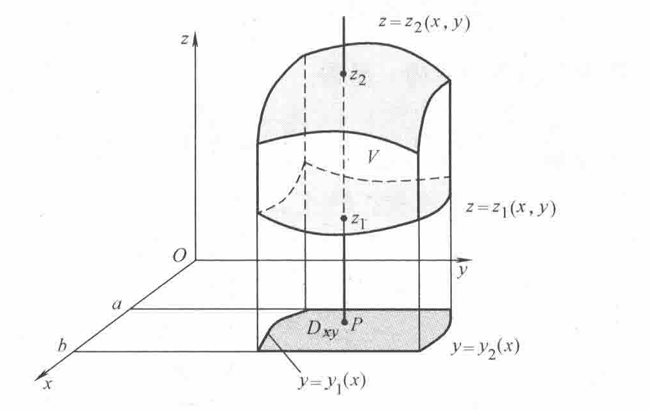
\includegraphics{2.6-3.png}
\end{center}
即先确定底面投影区域 $D$，再在每一点 $(x,y)$ 处 $z$ 从下曲面跑到上曲面，那么三重积分便化为
\[
\iiint_\Omega f(x,y,z)\,\mathrm{d}V
= \iint_D \left(\int_{z_1(x,y)}^{z_2(x,y)} f(x,y,z)\,\mathrm{d}z\right)\mathrm{d}A.
\]

其中 $\mathrm{d}A$ 就是底面上的面积微元。这句式并不陌生：先沿竖直方向把一根小柱上的贡献加起来，再让这根柱扫过整个底面。当然，你也可以按其他顺序投影——先固定 $z$ 看水平截面，或者先固定 $x$ 看 $yz$ 平面上的切片，全看区域长什么形状。

但空间中的区域往往不是方块。遇到圆柱、球体、圆锥这些带对称性的形体时，直角坐标就像用方榫去凿圆孔——能行，但很别扭。这时候柱坐标系和球坐标系便站出来说：换我试试。

柱坐标系其实是在极坐标的基础上加一个高度。令
\[
x = r\cos\theta,\quad y = r\sin\theta,\quad z = z,
\]
其中 $r\ge 0$，$0\le\theta<2\pi$，$z\in\mathbb{R}$。这里 $r,\theta$ 管着水平面，$z$ 管着竖直方向。和二重积分的极坐标一样，水平面的面积微元是 $r\,\mathrm{d}r\,\mathrm{d}\theta$，再乘上竖直方向的 $\mathrm{d}z$，就得到柱坐标下的体积微元：
\[
\mathrm{d}V = r\,\mathrm{d}r\,\mathrm{d}\theta\,\mathrm{d}z.
\]
\begin{center}
  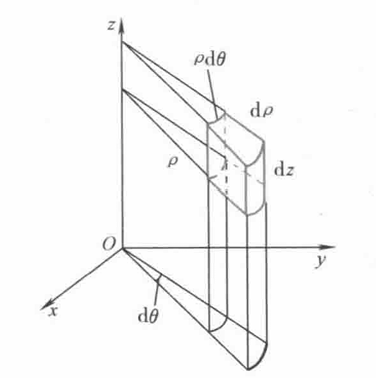
\includegraphics{2.6-4.png}
\end{center}

那个 $r$ 又来提醒你：远离 $z$ 轴的地方，同样大小的 $\mathrm{d}\theta$ 会扫出更长的弧。若区域在柱坐标下表示为
\[
\Omega = \{(r,\theta,z)\mid \alpha\le\theta\le\beta,\ r_1(\theta)\le r\le r_2(\theta),\ z_1(r,\theta)\le z\le z_2(r,\theta)\},
\]
则
\[
\iiint_\Omega f(x,y,z)\,\mathrm{d}V
= \int_{\alpha}^{\beta}\int_{r_1(\theta)}^{r_2(\theta)}\int_{z_1(r,\theta)}^{z_2(r,\theta)}
f(r\cos\theta,r\sin\theta,z)\; r\,\mathrm{d}z\,\mathrm{d}r\,\mathrm{d}\theta.
\]

\begin{center}
  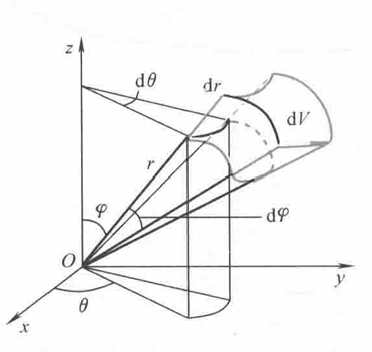
\includegraphics{2.6-5.png}
\end{center}


球坐标系则走得更远——它干脆把整个空间用半径和两个角度来刻画。令
\[
x = \rho\sin\phi\cos\theta,\quad y = \rho\sin\phi\sin\theta,\quad z = \rho\cos\phi,
\]
其中 $\rho\ge 0$ 是到原点的距离，$0\le\phi\le\pi$ 是与 $z$ 轴正方向的夹角（叫做极角），$0\le\theta<2\pi$ 是方位角。球坐标下的体积微元推导起来要多想一步：一个很小的区域近似于一个长方体，三条边的长度分别是 $\mathrm{d}\rho$、$\rho\,\mathrm{d}\phi$（沿着经线方向）、$\rho\sin\phi\,\mathrm{d}\theta$（沿着纬线方向），因此
\[
\mathrm{d}V = \rho^2\sin\phi\,\mathrm{d}\rho\,\mathrm{d}\phi\,\mathrm{d}\theta.
\]
$\rho^2\sin\phi$ 不是凭空冒出来的，它反映了距离原点越远，同样大小的角度变化扫过的弧长就越长这一几何事实。若区域在球坐标下简单（例如球体、球壳、圆锥面围出的部分），则
\[
\iiint_\Omega f(x,y,z)\,\mathrm{d}V
= \int_{\theta_1}^{\theta_2}\int_{\phi_1(\theta)}^{\phi_2(\theta)}\int_{\rho_1(\phi,\theta)}^{\rho_2(\phi,\theta)}
f(\rho\sin\phi\cos\theta,\rho\sin\phi\sin\theta,\rho\cos\phi)\;
\rho^2\sin\phi\;\mathrm{d}\rho\,\mathrm{d}\phi\,\mathrm{d}\theta.
\]

做柱坐标或球坐标的积分时，容易出错的地方其实和二重积分的极坐标完全一致：区域边界要写成新坐标下的范围，被积函数里的 $x,y,z$ 要替换干净，而体积微元里多出来的因子（柱坐标的 $r$，球坐标的 $\rho^2\sin\phi$）绝不能随手丢掉。很多人算出的错误答案，不是积分技术不行，而是在变量代换的瞬间没有真正接受“坐标系换了，度量也跟着变了”这件事——就像你在不同的地图上测量距离，用的尺子刻度是不一样的。

从二重积分到三重积分，从直角坐标到柱坐标、球坐标，你会发现数学里并没有那么多新东西。定义只有一种——把区域切成小块，求和，取极限。但坐标系可以有多种，每一种都在说：我帮你把区域的对称性翻译成最简单的积分限。理解了这个，所谓“重积分”就不再是一堆公式的堆叠，而是一套可以根据几何形状灵活切换的语言。



\chapter{线性代数}

如果群论是自然界偏爱对称性的签名，概率论是复杂系统粗粒化的通用语言，那么线性代数就是这一切的底层操作系统。它朴素到了近乎谦卑的程度——研究的无非是线性方程组、矩阵乘法和向量空间——但几乎每一种重要的数学结构在某个层次上都是线性空间的某种推广。线性代数的威力，在于它抓住了“线性”这个自然界最普遍也最简单的近似模式，然后用一整套干净利落的代数工具把它武装到了极致。

线性代数最早的推力来自坐标系变换。笛卡尔把几何放进坐标系，牛顿和莱布尼茨用微积分描述曲线，到了十九世纪，数学家们开始意识到：选什么样的坐标系不是无关紧要的，而坐标变换本身就携带着深刻的几何信息。当笛卡尔平面上的一条椭圆在标准坐标轴下表示为 $\frac{x^2}{a^2}+\frac{y^2}{b^2}=1$ 时，它看起来有点复杂；但只要把坐标轴旋转到椭圆的主轴方向，它立刻就变成最简单的形式。这个旋转就是线性代数中的正交对角化\textsuperscript{[\pageref{diag}]}：找一个正交矩阵 $Q$，使得 $Q^T A Q=\Lambda$ 成为对角阵，其中 $A$ 是二次型矩阵，$\Lambda$ 的对角元就是主轴长度平方的倒数。坐标变换不止是重新画网格，而是把几何对象从“斜着看”掰正了看，从而把纠缠在一起的方向拆成独立伸缩的维度。这个思想贯穿了全部线性代数：选对了基，一切都会变得简单。

如果说坐标系变换给出了线性代数的几何直觉，那么数列和递推则给了它一个通向离散动力学的入口。斐波那契数列的递推 $F_{k+2}=F_{k+1}+F_k$ 是一个二阶线性递推，写成矩阵形式就是
\[
\begin{pmatrix}F_{k+2}\\F_{k+1}\end{pmatrix}=
\begin{pmatrix}1&1\\1&0\end{pmatrix}
\begin{pmatrix}F_{k+1}\\F_k\end{pmatrix}.
\]
转移矩阵 $A$ 的特征值是 $\frac{1+\sqrt{5}}{2}$ 和 $\frac{1-\sqrt{5}}{2}$，对角化后通项公式一举写出：$F_k=\frac{1}{\sqrt{5}}(\lambda_1^k-\lambda_2^k)$。一个只看递推觉得不可思议的无理数通项，在特征向量构成的基下不过是两个等比数列的叠加。$k$ 步的演化不过是把初始状态在这组基上投影，在每个方向上伸缩对应特征值的 $k$ 次幂，再合回来。这层图景抽象出来就是一个普适框架：线性递推、微分方程组、马尔可夫链的平稳分布、PageRank 算法的迭代——全部都是同一个故事的不同版本：把变换对角化（或者变成若尔当形），然后看它在每个特征方向上伸缩。

物理学给线性代数递来了最华丽的请帖。量子力学的一开始，海森堡的矩阵力学就把物理量直接定义为矩阵。薛定谔的波动力学看似不同，但两人很快就证明了它们是等价的——一个用矩阵语言说话，一个用微分算子语言说话，而线性代数恰恰坐在它们中间。量子态是希尔伯特空间里的向量，可观测量的测量值是算符的特征值，系统的演化是酉矩阵的作用。狄拉克那本《量子力学原理》基本上是线性代数在物理空间中的一次辉煌展开。经典物理学同样充斥线性结构：刚体转动惯量是一个对称矩阵，它的特征向量是主轴方向，特征值是主转动惯量；弹性体中应力张量和应变张量通过一个四阶张量相联——在各向同性近似下退化为两个拉梅常数，但本质上仍然是线性算符在起作用。无论经典还是量子，物理学像是一部用线性代数谱写的交响曲：方程可以是偏微分的，可以是积分的，但剪开了看，大多数物理理论中真正能精确求解的核心部分，都是线性的。

化学同样离不开线性代数，只不过是悄悄地用。分子轨道理论中的分子轨道是原子轨道的线性组合：设原子轨道为基函数 $\chi_1,\dots,\chi_n$，分子轨道 $\psi_i$ 写为 $\psi_i=\sum_{\mu}c_{\mu i}\chi_\mu$。系数 $c_{\mu i}$ 由哈特里-福克方程 $FC=SC\varepsilon$ 迭代求解，其中 $F$ 是福克矩阵，$S$ 是重叠矩阵——两个矩阵都是对称的，求解本质上就是广义特征值问题 $F\mathbf{c}=\varepsilon S\mathbf{c}$。化学家用这个框架预测化学键的强度、分子的偶极矩、激发的能级跃迁。量子化学的另一个核心任务是振动分析：分子的谐振近似振动频率是海森矩阵（势能对核坐标的二阶导数矩阵）的特征值的平方根。苯的六个碳原子拉伸和弯曲振动模式被点群表示和矩阵对角化联合分类，红外光谱中哪些峰出现，哪几个是二重简并的，早在实验测量之前就已经由矩阵的特征结构决定了。化学家每天面对分子轨道能级图，那不过是一张排列整齐的特征值表，只是画成了竖线。

从坐标旋转到斐波那契数列，从量子态到分子轨道，线性代数把表面上彼此无关的问题翻译成同一套语法：向量空间、线性变换、特征值、对角化。初学者容易把它当成一堆矩阵乘法和行列式的枯燥规则来记忆，那样就会错过它的真正用途。它的本质并不复杂：把正确的问题写在正确的基下，答案常常自己浮现在对角线上。这句话在几何中成立，在数列中成立，在量子力学中成立，在化学计算中成立——这本身，就是线性代数最值得被记住的地方。

\subsection*{三种基本变换：线性代数的操作算子}

如果说线性代数的核心是“用基的观点看问题”，那么\textbf{变换}就是“在不同视角之间切换的操作”。初等变换、合同变换、相似变换分别对应着不同层面上的视角迁移。

\paragraph{初等变换\textsuperscript{[\pageref{Elementary_Transformation}]}（Elementary Transformation）}
操作方式是三种基本行操作（或列操作）：交换两行、某行乘以非零常数、某行加上另一行的倍数。它保持矩阵的秩、行空间和零空间不变，核心作用是解线性方程组、求逆矩阵和计算行列式。初等变换是最“底层”的操作——它不关心矩阵是否对称，也不关心是否保持几何距离，只是在数值上老老实实地把矩阵掰成行阶梯形。

\paragraph{合同变换\textsuperscript{[\pageref{Congruence_Transformation}]}（Congruence Transformation）}
形式上为 $B = C^T A C$，其中 $C$ 可逆。它要求“行、列同步操作”：对矩阵做了什么列变换，就要立刻对行做完全相同的变换。这个约束听起来有点麻烦，却换来一个宝贵的性质——保持对称矩阵的对称性，以及更深刻的\textbf{惯性定理}：正特征值个数、负特征值个数、零特征值个数在合同变换下纹丝不动。合同变换的任务是“化简二次型”：把 $x^T A x$ 变成 $y^T \Lambda y$，让纠缠在一起的交叉项消失。它不保持特征值的大小（特征值可以变），但死死守护住特征值的\textbf{符号分布}。

\paragraph{相似变换\textsuperscript{[\pageref{Similarity_Transformation}]}（Similarity Transformation）}
形式上为 $B = P^{-1} A P$，其中 $P$ 可逆。这是三种变换中最“豪华”的一种，因为它要求的条件最强：左乘的是 $P^{-1}$，右乘的是 $P$——两边的矩阵互为逆。几何上，相似变换描述的是\textbf{同一个线性变换在不同坐标系下的表达}。矩阵 $A$ 和 $B$ 本质上是同一个线性映射，只是观察的基不同。因此相似变换守护的是线性变换的\textbf{本质属性}：特征值、行列式、迹、秩、最小多项式——所有不依赖于坐标的东西都不动。对数学家而言，两个矩阵如果相似，它们就是“同一个东西穿上不同的衣服”。对角化 $P^{-1}AP = \Lambda$ 就是相似变换最华丽的应用：把矩阵写成特征值的集合，每个特征方向独立伸缩。

\begin{table}[H]
  \centering
  \renewcommand{\arraystretch}{1.4}
  \begin{tabular}{l|c|c|l}
    \toprule
    变换类型 & 公式 & 是否改变特征值？ & 保持的不变量 \\
    \midrule
    初等行变换（单独） & $EA$ & 改变（无规律） & 秩 \\
    初等列变换（单独） & $AE$ & 改变（无规律） & 秩 \\
    相似变换 & $P^{-1}AP$ & 不改变 & 特征值、秩、迹、行列式 \\
    合同变换（一般情况） & $C^{\!T}AC$ & 改变 & 惯性指数、对称性、秩 \\
    正交合同变换（$C^{\!T}=C^{-1}$） & $Q^{\!T}AQ$ & 不改变 & 特征值、惯性指数（此时两者等价） \\
    \bottomrule
  \end{tabular}
  \caption{三种变换对特征值的影响对比}
\end{table}


从线性方程组到二次型分类，从量子态演化到分子振动模式，这三种变换轮流登场。学线性代数到后来会发现：大部分定理无非是在问——在这个问题里，我允许用哪一种变换？保持哪些量不变？然后答案就会沿着那些不变量自然而然地浮现出来。

\newpage

\section{方程组}


如果你第一次接触线性方程组，很容易觉得这不过是“把几个未知数解出来”的技术题。可只要再多看一步，你就会发现它讨论的其实是一件更深的事：许多个线性条件同时加在一起，究竟还能给变量留下多少活动空间。于是线性方程组的核心问题，从来不只是算得快不快，而是这些条件彼此之间是独立的、重复的，还是互相冲突的。

最简单的情形当然是二元一次方程组
\begin{equation*}
\begin{cases}
 a_1x+b_1y=c_1,\\
 a_2x+b_2y=c_2.
\end{cases}
\end{equation*}
在这个层面上，我们从小学起就已经熟悉消元法了。若
\[
a_1b_2-a_2b_1\neq 0,
\]
那么两个方程提供的是两条彼此独立的约束，于是方程组有唯一解，而且可以显式写成
\begin{equation*}
 x=\frac{c_1b_2-c_2b_1}{a_1b_2-a_2b_1},\qquad
 y=\frac{a_1c_2-a_2c_1}{a_1b_2-a_2b_1}.
\end{equation*}
这个公式本身并不神秘，它只是告诉你：当两条约束真的在“不同方向”上发力时，交点就被唯一钉住了。

可是一旦未知元多起来，继续靠手工追着某个变量逐个消去，就会越来越混乱。比如考虑下面这个四元线性方程组：
\begin{equation*}
\begin{cases}
x+y+z+w=10,\\
2x-y+3z+2w=15,\\
-x+4y+z-w=5,\\
3x+y+2z+4w=20.
\end{cases}
\end{equation*}
这时候真正该注意到的一点是：在整个消元过程中，我们并不关心未知元本身长什么样，真正被加工的是它们前面的系数。因此，把方程组压缩成一张数表是很自然的想法，这张表就是增广矩阵：
\[
\left[
\begin{array}{cccc|c}
1&1&1&1&10\\
2&-1&3&2&15\\
-1&4&1&-1&5\\
3&1&2&4&20
\end{array}
\right].
\]
竖线左边是系数矩阵，右边是常数列；而单独把左边拿出来，就得到系数矩阵。从这个视角看，高斯消元法其实不再是“算术技巧”，而是在做一种系统整理：用初等行变换把一团纠缠的线性条件，一步步改写成层次分明、可以从下往上读的结构。

高斯消元通常分成两步：先消元，再回代。所谓消元，就是沿着一列一列往下走，每次选定一个主元，然后把这一列主元以下或周围不需要的项消掉，让矩阵逐渐逼近阶梯形。对上面的例子，消元过程可以写成
\[
\resizebox{\textwidth}{!}{$
\left[
\begin{array}{cccc|c}
1&1&1&1&10\\
2&-1&3&2&15\\
-1&4&1&-1&5\\
3&1&2&4&20
\end{array}
\right]
\xrightarrow{\substack{R_2\leftarrow R_2-2R_1\\R_3\leftarrow R_3+R_1\\R_4\leftarrow R_4-3R_1}}
\left[
\begin{array}{cccc|c}
1&1&1&1&10\\
0&-3&1&0&-5\\
0&5&2&0&15\\
0&-2&-1&1&-10
\end{array}
\right]
\xrightarrow{\substack{R_3\leftarrow 3R_3+5R_2\\R_4\leftarrow 3R_4-2R_2}}
\left[
\begin{array}{cccc|c}
1&1&1&1&10\\
0&-3&1&0&-5\\
0&0&11&0&20\\
0&0&-5&3&-20
\end{array}
\right]
\xrightarrow{R_4\leftarrow 11R_4+5R_3}
\left[
\begin{array}{cccc|c}
1&1&1&1&10\\
0&-3&1&0&-5\\
0&0&11&0&20\\
0&0&0&33&-120
\end{array}
\right]
$}
\]
做到这里，其实最困难的部分已经结束了。因为矩阵一旦变成这种上三角的阶梯结构，方程的层级关系就清楚了：最后一行先决定最后一个主元，再一层层往回带，于是就得到
\[
\left(x,y,z,w\right)=\left(\frac{105}{11},\frac{25}{11},\frac{20}{11},-\frac{40}{11}\right).
\]
这个例子给出了唯一解，但千万别误以为线性方程组总会这么听话。唯一解其实只是若干可能性中的一种。一个方程组还可能无解，也可能有无穷多解；而高斯消元法的真正威力，恰恰在于它不仅能“算解”，还能把这三种情况清清楚楚地区分出来。

为了看清这一点，不妨比较下面两个增广矩阵：
\[
\left[
\begin{array}{cccc|c}
1&1&1&1&10\\
0&-3&1&0&-5\\
0&0&11&0&20\\
0&0&0&0&-120
\end{array}
\right]
\qquad
\left[
\begin{array}{cccc|c}
1&1&1&1&10\\
0&-3&1&0&-5\\
0&0&11&0&20\\
0&0&0&0&0
\end{array}
\right].
\]
它们看上去只差最后一行，可几何意义完全不同。左边这个矩阵对应的最后一行实际上是
\[
0 \times x_4=-120,
\]
它提供了一个不真实的约束，所以它是无解的。

而右边这个矩阵的最后一行却退化成了
\[
0=0,
\]
也就是说，最后一个条件根本没有提供新信息，于是变量里会有一个方向没有被完全约束住，这时就会出现无穷多解。对于无穷多解的情形，我们可以把没有主元的变量看成自由变量，也就是你可以任意指定它的值，其余变量再被迫跟着调整。若取 $x_4$ 为自由变量，那么方程组就变成
{\renewcommand{\arraystretch}{1.45}
\[
\begin{cases}
 x_1+x_2+x_3+x_4=10\\
 -3x_2+x_3=-5\\
 11x_3=20\\
0=0
\end{cases}
\xrightarrow{\text{取 }x_4\text{ 为自由变量}}
\begin{cases}
 x_1+x_2+x_3=10-x_4\\
 x_2=\frac{25}{11}\\
 x_3=\frac{20}{11}
\end{cases}
\xrightarrow{\text{回代求 }x_1}
\begin{cases}
 x_1=\frac{65}{11}-x_4\\
 x_2=\frac{25}{11}\\
 x_3=\frac{20}{11}
\end{cases}
\]
}
这说明解不是一个孤零零的点，而是一整族由参数控制的解。你随便给 $x_4$ 一个值，其他变量就随之确定。这里最值得记住的，不是具体算出了哪个分式，而是“自由变量”这个概念：当约束不够多时，解会保留若干自由方向，而这些自由方向正是线性代数以后要不断追踪的东西。

怎样把这种“约束够不够”的直觉量化下来？这就引出了秩。把\textbf{矩阵化为最简行阶梯形之后，非零行的个数，也就是主元的个数}，称为矩阵的秩。秩测量的不是矩阵有多大，而是它真正提供了多少个彼此独立的线性条件。于是，判断方程组解的类型，本质上就是比较这些独立条件的数目，究竟和未知元个数之间是什么关系。


\subsection{线性方程组的基本定理}

在数学上，主元的个数称为矩阵的秩；数值上它等于最简行阶梯矩阵中非零行的个数。通过比较系数矩阵的秩、增广矩阵的秩以及未知元个数，我们就能统一判断线性方程组到底有没有解、如果有，是唯一还是无穷多。这就是线性方程组的基本定理。

设线性方程组写为
\[
A\mathbf{x}=\mathbf{b},\qquad
\begin{pmatrix}
a_{11} & a_{12} & \cdots & a_{1n} \\
a_{21} & a_{22} & \cdots & a_{2n} \\
\vdots & \vdots & \ddots & \vdots \\
a_{m1} & a_{m2} & \cdots & a_{mn}
\end{pmatrix}
\begin{pmatrix}x_1 \\ x_2 \\ \vdots \\ x_n\end{pmatrix}
=
\begin{pmatrix}b_1 \\ b_2 \\ \vdots \\ b_m\end{pmatrix}
\]

其中 $A\in\mathbb{R}^{m\times n}$ 为系数矩阵，$[A\mid \mathbf{b}]$ 为增广矩阵。写成方程组的形式就是：

\[
A\mathbf{x}=\mathbf{b}\quad\Longleftrightarrow\quad
\left\{\begin{aligned}
a_{11}x_1 + a_{12}x_2 + \cdots + a_{1n}x_n &= b_1 \\
a_{21}x_1 + a_{22}x_2 + \cdots + a_{2n}x_n &= b_2 \\
\vdots\qquad \vdots\qquad \vdots\qquad \vdots &\qquad \vdots \\
a_{m1}x_1 + a_{m2}x_2 + \cdots + a_{mn}x_n &= b_m
\end{aligned}\right.
\]

当我们将增广矩阵$[A\mid \mathbf{b}]$化简成最简行阶梯型矩阵后，则有以下几种情况

\begin{enumerate}
  \item 当 $\operatorname{rank}(A)=\operatorname{rank}([A\mid \mathbf{b}])$ 时，方程组有解；
  \item 当 $\operatorname{rank}(A)<\operatorname{rank}([A\mid \mathbf{b}])$ 时，方程组无解；
  \item 当 $\operatorname{rank}(A)=\operatorname{rank}([A\mid \mathbf{b}])=r<n$ 时，方程组有无穷多解，自由变量个数为 $n-r$；
 \item 当 $\operatorname{rank}(A)=\operatorname{rank}([A\mid \mathbf{b}])=n$ 时，方程组有唯一解。
\end{enumerate}

这一定理给出了线性方程组“有解、无解、唯一解、无穷多解”的统一判别标准。说得再直白一点：先看系数矩阵本身能提供多少个独立约束，再看把常数项并进去以后会不会多出新的矛盾，最后再和未知元总数比较，就知道解空间还剩下多少自由度。和我们上一小节所作的事情一模一样。

但是我们总不能每次都通过化简矩阵来判断方程组解的情况吧，特别是遇到一些带未知数的系数矩阵，那样运算简直麻烦上天了。这就不由得提到我们后面会讲解的克拉默法则\textsuperscript{[\pageref{Cramer}]}了。它指出方程组的唯一解总可以由行列式确定：
\[
x_j=\frac{|A_j|}{|A|}= \frac{
\begin{vmatrix}
a_{11} & a_{12} & \cdots & b_1 & \cdots & a_{1n} \\
a_{21} & a_{22} & \cdots & b_2 & \cdots & a_{2n} \\
\vdots & \vdots & & \vdots & & \vdots \\
a_{n1} & a_{n2} & \cdots & b_n & \cdots & a_{nn}
\end{vmatrix}
}{
\begin{vmatrix}
a_{11} & a_{12} & \cdots & a_{1n} \\
a_{21} & a_{22} & \cdots & a_{2n} \\
\vdots & \vdots & \ddots & \vdots \\
a_{n1} & a_{n2} & \cdots & a_{nn}
\end{vmatrix}
}, \quad j = 1, 2, \dots, n,
\]
这样我们只需要判断行列式$|A|$的情况就可以快速判断方程组是有唯一解还是无穷多解。





\subsection{线性方程组的解：从秩到零空间}
不过秩的意义并不止于“判断方程组有没有解”。它还是描述线性变换复杂程度的一个基本数量，因此在矩阵运算里也不断出现。下面这些性质都非常常用，比较显然的，单纯由定义所引出的：
\[
0\le \operatorname{rank}(A)\le \min\{m,n\}.
\]
\[
\operatorname{rank}(A+B)\le \operatorname{rank}(A)+\operatorname{rank}(B).
\]

另外还有学习向量空间后可以得到的：
\[
\operatorname{rank}(A)+\operatorname{rank}(B)-n
\le \operatorname{rank}(AB)
\le \min\{\operatorname{rank}(A),\operatorname{rank}(B)\},
\]
这个不等式本质上描述了$B$的列向量都是$A$的零空间的解的情形，也就是接下来我们要讲的。

如果你第一次认真看线性方程组，你很容易把它误会成一堆枯燥的消元技巧：把这一行减去那一行，把这个未知元消掉，再把另一个未知元解出来，好像整件事只是算术的耐心活。但如果稍微退后一步，你会发现它真正讨论的根本不是“怎么解几个数”，而是“一个变换到底压扁了空间的哪些方向，又保留了哪些方向”。这才是线性方程组真正迷人的地方。
我们考虑方程组
\[
A\mathbf{x}=\mathbf{b}.
\]
这里矩阵 $A$ 可以看成一台机器：你把一个向量 $\mathbf{x}$ 塞进去，它吐出来一个新的向量 $\mathbf{b}$。于是“求解方程组”这件事，本质上就是在问：\textbf{什么样的输入，会被这台机器送到指定的输出？}

先看最简单也最重要的情形：齐次方程组
\[
A\mathbf{x}=\mathbf{0}.
\]
这时我们问的是：哪些向量一旦进入这台机器，就会被它彻底压成零？所有这样的向量组成的集合，就叫做矩阵 $A$ 的\textbf{零空间}\label{kernel}，记作
\[
N(A)=\{\mathbf{x}\mid A\mathbf{x}=\mathbf{0}\}.
\]
零空间不是随便一个点集，它本身就是一个向量空间。因为如果两个向量都会被压成零，那么它们的和、它们的数乘，当然也还是会被压成零。换句话说，零空间记录了这台线性机器“看不见”的全部方向：沿着这些方向你怎么动，它都分辨不出来。

这时候秩就出场了。矩阵的秩 $\operatorname{rank}(A)$ 描述的是这台机器真正能输出多少维独立的信息。若 $A$ 是一个 $m\times n$ 矩阵，那么输入空间本来有 $n$ 个自由方向；其中有一部分方向被机器保留下来，形成像空间的维数，也就是秩；另一部分方向被机器压扁，落入零空间。于是一个极其深刻又极其自然的关系出现了：
\[
\dim N(A)+\operatorname{rank}(A)=n.
\]
这就是秩—零度定理。它说得很朴素：一个线性变换不可能既保留所有方向，又把所有方向都压掉；输入空间的总自由度，恰好分成“被看见的部分”和“被抹掉的部分”。

现在再回到一般方程组$A\mathbf{x}=\mathbf{b}$,
这里首先要问的，不是怎么解，而是\textbf{有没有解}。这就取决于 $\mathbf{b}$ 是否落在 $A$ 的列空间里。
对于 $A = \begin{pmatrix} \mathbf{a}_1 & \mathbf{a}_2 & \cdots & \mathbf{a}_n \end{pmatrix}$，其中 $\mathbf{a}_j \in \mathbb{R}^m$ 是 $A$ 的列向量。
$A$ 的\textbf{列空间}\label{cspace}（column space）定义为所有形如 $A\mathbf{x}$ 的向量构成的集合：
\[
\operatorname{Col}(A) = \left\{ \sum_{j=1}^{n} x_j \mathbf{a}_j \;\big|\; x_1,\ldots,x_n \in \mathbb{R} \right\} = \operatorname{span}\{\mathbf{a}_1, \mathbf{a}_2, \ldots, \mathbf{a}_n\} \subseteq \mathbb{R}^m.
\]
$\operatorname{Col}(A)$ 是 $\mathbb{R}^m$ 中由 $A$ 的所有列向量张成的子空间\textsuperscript{[\pageref{space}]}。线性方程组 $A\mathbf{x} = \mathbf{b}$ 有解当且仅当 $\mathbf{b} \in \operatorname{Col}(A)$，即 $\mathbf{b}$ 落在列向量张成的平面、超平面或整个空间中。


这件事在计算上体现为增广矩阵的秩判别：
\[
A\mathbf{x}=\mathbf{b}\ \text{有解}
\quad\Longleftrightarrow\quad
\operatorname{rank}(A)=\operatorname{rank}(A,\mathbf{b}).
\]
这个条件非常像一条边境线：只要把 $\mathbf{b}$ 加进来没有制造出新的独立信息，那么它原本就在列空间里；如果秩突然增大，说明它是个“外来者”，不属于这个系统原有的输出世界。

一旦有解，下一件最重要的事就是理解：\textbf{所有解长什么样？} 这恰恰是零空间出场的地方。设 $\mathbf{x}_p$ 是方程组的一个特解，即
\[
A\mathbf{x}_p=\mathbf{b}.
\]
如果 $\mathbf{x}$ 是任何另一个解，那么
\[
A\mathbf{x}=\mathbf{b}.
\]
两式相减就得到
\[
A(\mathbf{x}-\mathbf{x}_p)=\mathbf{0}.
\]
也就是说，任意两个解的差一定落在零空间里。于是所有解都可以写成
\[
\mathbf{x}=\mathbf{x}_p+\mathbf{x}_h,
\qquad \mathbf{x}_h\in N(A).
\]
这就是线性方程组解的结构。它的意思非常漂亮：一个非齐次方程组的全部解，不是散落的许多孤立点，而是“一个特解”沿着“零空间”整个平移出去得到的几何对象。若零空间只有零向量，那么解只有一个；若零空间是一条直线，那么全部解就是沿某个方向排开的直线；若零空间是一个平面，那么全部解就是一个平移了的位置平面。所谓“自由变量”，本质上正是在给零空间选参数。

因此，齐次方程组和非齐次方程组之间的关系，也一下子变得透明了：齐次方程组给出的是骨架，是方向，是所有可能发生平移的内部结构；非齐次方程组只是在这个骨架上挑了一个落点，然后把整个骨架搬过去。你可以把它想成一盏灯照在空间里：零空间是那条永远投不出影子的暗方向，而特解则是你在亮处先找到的一个具体位置。

这也解释了为什么我们在解方程组时总要把矩阵化成行最简阶梯形。表面上看，我们只是在做消元；但从结构上看，我们是在把这台机器的内部线路一点点扒开。主元列告诉我们哪些方向真的贡献了独立信息，自由变量告诉我们哪些方向属于零空间，而零空间的维数正是未知量个数减去主元个数，也就是
\[
\dim N(A)=n-\operatorname{rank}(A).
\]
所以行化简并不是机械的算术体操，它是在给空间做解剖：哪些方向能被机器识别，哪些方向会被吞掉，哪些输出可以达到，哪些根本到不了，全都在化简后的矩阵里暴露无遗。

最后，把这些话收成一句最值得记住的结论：\textbf{秩决定这台线性机器能传递多少独立信息，零空间决定它会丢掉多少独立信息，而线性方程组的全部解，就是一个特解加上所有被它丢掉的方向。} 一旦这样去看，线性方程组就不再只是若干个 $x,y,z$ 的求值问题，而变成了空间、方向、压缩与信息之间的一场非常优雅的对话。

讲完了零空间和特解的结构，接下来的问题自然就是：这两个东西具体怎么求？抽象的理论固然漂亮，但你若真要解一个方程组，总得有一套能落到纸面上的办法。

先看齐次方程组 $A\mathbf{x}=\mathbf{0}$。我们要找到所有被矩阵压成零向量的 $\mathbf{x}$，也就是零空间。做法并不神秘：把矩阵 $A$ 化成行最简阶梯形。设 $A$ 是 $m\times n$ 矩阵，经过行化简后得到形如
\[
\left[\begin{array}{cccccc}
1 & 0 & \cdots & 0 & a_{1,k_1} & \cdots \\
0 & 1 & \cdots & 0 & a_{2,k_2} & \cdots \\
\vdots & \vdots & \ddots & \vdots & \vdots & \\
0 & 0 & \cdots & 1 & a_{r,k_r} & \cdots \\
0 & 0 & \cdots & 0 & 0 & \cdots \\
\end{array}\right]
\]
的形式，其中每行第一个非零元（主元）所在的列称为主元列，其余列称为自由列。主元列的个数就是秩 $r$，自由列的个数就是 $n-r$，也就是零空间的维数。

现在把自由列对应的变量叫做自由变量——它们可以自由取值，不受约束。对于每一个自由变量，我们做这样一件事：把它取 $1$，其他自由变量取 $0$，然后回代到行最简形方程组中，依次解出主元变量。这样一来，每个自由变量就对应零空间中的一个基向量。把这些基向量拼在一起，零空间就是它们的全部线性组合。

举个例子会更清楚。设行化简后得到
\[
\begin{cases}
x_1 + 2x_3 - x_4 = 0,\\
x_2 + 3x_3 + x_4 = 0.
\end{cases}
\]
这里 $x_1,x_2$ 是主元变量（对应主元列），$x_3,x_4$ 是自由变量。先令 $x_3=1,x_4=0$，代入解得 $x_1=-2,x_2=-3$，得到一个向量 $(-2,-3,1,0)^T$。再令 $x_3=0,x_4=1$，解得 $x_1=1,x_2=-1$，得到 $(1,-1,0,1)^T$。于是零空间为
\[
N(A)=\left\{c_1\begin{pmatrix}-2\\-3\\1\\0\end{pmatrix}+c_2\begin{pmatrix}1\\-1\\0\\1\end{pmatrix}\;\middle|\;c_1,c_2\in\mathbb{R}\right\}.
\]
你看，整个过程的逻辑并不复杂：自由变量就是你可以随意拨动的旋钮，每一个旋钮给出一维的行走方向，而零空间正是这些方向张成的所有可能移动。

上面的回代法在理论上清晰，但手动操作时每次都要重新列方程、回代，略显繁琐。工程线性代数中有一个更“懒”的办法——把列重新排一排，让行最简阶梯形呈现一个天然的分块结构，零空间的基向量就可以一口报出来。

具体操作分三步：

第一步，将行最简阶梯形 $R$ 的列重新排列，把所有主元列移到最前面，所有自由列放在后面。重排后的矩阵呈分块形式
\[
R'=\left[\begin{array}{c|c}
I_r & F\\
\hline
0 & 0
\end{array}\right],
\]
其中 $I_r$ 是 $r\times r$ 单位矩阵（对应 $r$ 个主元列），$F$ 是 $r\times (n-r)$ 矩阵（主元行与自由列交叉处的那些系数，带上原本的正负号），底下是全零行。

第二步，观察分块结构。原方程 $R\mathbf{x}=\mathbf{0}$ 经列重排后变为 $R'\mathbf{x}'=\mathbf{0}$，其中 $\mathbf{x}'$ 是变量按同样顺序重排后的向量。写成分块形式：
\[
\left[\begin{array}{c|c}
I_r & F\\
\hline
0 & 0
\end{array}\right]
\begin{pmatrix}\mathbf{x}_P\\\hline\mathbf{x}_F\end{pmatrix}
=\mathbf{0}
\quad\Longrightarrow\quad
I_r\mathbf{x}_P+F\mathbf{x}_F=\mathbf{0}
\quad\Longrightarrow\quad
\mathbf{x}_P=-F\,\mathbf{x}_F.
\]
这里 $\mathbf{x}_P$ 是主元变量排成的向量，$\mathbf{x}_F$ 是自由变量排成的向量。方程告诉我们：主元变量完全由自由变量决定，且关系正好是 $\mathbf{x}_P=-F\mathbf{x}_F$。

第三步，把自由变量的一组标准基代入，直接写出零空间基。令 $\mathbf{x}_F$ 依次取 $\mathbf{e}_1,\mathbf{e}_2,\dots,\mathbf{e}_{n-r}$（即每次一个自由变量取 $1$，其余取 $0$），对应的 $\mathbf{x}_P=-F\mathbf{e}_i$ 恰好就是 $-F$ 的第 $i$ 列。于是在重排后的变量顺序下，零空间的基向量为
\[
\begin{pmatrix}-F\\\hline I_{n-r}\end{pmatrix}
\]
的各列——上面是 $-F$ 的对应列，下面是单位矩阵的对应列。写成完整矩阵形式：
\[
N(R')=\operatorname{col}\begin{pmatrix}-F\\ I_{n-r}\end{pmatrix}.
\]

最后，把变量顺序恢复成原来的排列即可。列的排列对应变量的排列，恢复顺序就是把上面得到的基向量的分量按原顺序重新排排位置。这一步是纯机械操作，不会出错。

回到刚才的例子。行最简形对应的增广矩阵信息为：
\[
R=\left[\begin{array}{cc|cc}
1&0&2&-1\\
0&1&3&1
\end{array}\right],
\]
主元列是第 $1,2$ 列，自由列是第 $3,4$ 列。此时列已经天然排好了——主元列在前，自由列在后，不需要重排。$I_2$ 就是左边的 $2\times2$ 单位阵，$F=\begin{bmatrix}2&-1\\3&1\end{bmatrix}$。于是
\[
-F=\begin{bmatrix}-2&1\\-3&-1\end{bmatrix},\qquad I_2=\begin{bmatrix}1&0\\0&1\end{bmatrix}.
\]
直接读出零空间基（在重排后的变量顺序 $(x_1,x_2,x_3,x_4)$ 下）为
\[
\begin{pmatrix}-F\\ I_2\end{pmatrix}=
\begin{bmatrix}
-2 & 1\\
-3 & -1\\
1 & 0\\
0 & 1
\end{bmatrix}.
\]
这两列恰好就是我们之前回代得到的两个基向量 $(-2,-3,1,0)^T$ 和 $(1,-1,0,1)^T$——一个不多，一个不少。


回代法让你看到每一个自由变量如何一步步“牵动”主元变量，适合理解零空间的几何构造；排列法让你直接写出答案，适合快速手算和编程实现。无论用哪种，本质都是同一件事：自由变量是零空间的坐标轴，主元变量被这些坐标轴线性地决定了。秩告诉你矩阵“真正起作用”的维度，零空间则告诉你“被压扁”的那些方向——它们合在一起，完整描述了线性变换 $A\mathbf{x}$ 的结构。

现在来看非齐次方程组 $A\mathbf{x}=\mathbf{b}$。解的结构已经说过：全部解 = 一个特解 + 零空间。那么特解怎么找？还是回到行最简阶梯形，但现在要把 $\mathbf{b}$ 也带进来。

把增广矩阵 $(A\mid\mathbf{b})$ 化成行最简形。做法和齐次时几乎一样，唯一的区别是最后一列多了一个常数。关键的一步是：把所有自由变量都设为 $0$。为什么？因为自由变量对应的是零空间的方向，而我们此刻只想要一个“落点”，不需要任何来自零空间的偏移。设自由变量为 $0$ 之后，剩下的主元方程组就变成了一个三角形系统，从最后一个主元开始逐个回代，就能解出所有主元变量的值。这样得到的 $\mathbf{x}_p$ 就是一个特解。

还是用上面的例子，但这次加上右端项。设增广矩阵化成了
\[
\begin{cases}
x_1 + 2x_3 - x_4 = 3,\\
x_2 + 3x_3 + x_4 = 1.
\end{cases}
\]
自由变量仍为 $x_3,x_4$。令 $x_3=0,x_4=0$，立即得到 $x_1=3,x_2=1$，所以一个特解为 $(3,1,0,0)^\top$。于是全部解就是
\[
\mathbf{x}= \begin{pmatrix}3\\1\\0\\0\end{pmatrix} + c_1\begin{pmatrix}-2\\-3\\1\\0\end{pmatrix} + c_2\begin{pmatrix}1\\-1\\0\\1\end{pmatrix}.
\]

你可能会问：如果自由变量不设零而设别的数，会怎样？也能得到特解，但得到的会是另一个不同的特解——它在零空间方向上平移了一下。这并不错，只是得到的表达式中系数不再刚好是自由变量本身，形式上会乱一些。所以设自由变量为 $0$ 无非是最干净、最省事的约定。

至此，整个求解的过程就完整了：行化简是为了看清主元列和自由列；从齐次方程组得到零空间的基，从非齐次方程组得到一个特解；然后两者相加，就是全部解。这套步骤并不需要你背口诀，它的每一步都有几何意义在下面托着：主元列是机器真正“看见”的方向，自由列是机器“看不见”的方向，特解是在列空间里随便找一个目标点的输入，而零空间则是那些不改变输出的所有暗方向。

把这些话收在一起，也许你就能理解为什么线性代数的教材总在反复念叨“秩—零度定理”“行最简形”“自由变量”这些东西。它们不是彼此孤立的技巧，而是一个共同的故事：线性变换把输入空间压出一个像空间和一个零空间，解方程就是在问“给定输出，哪些输入能到达它”，而答案永远是“一个落脚点加上全部可以被压扁的方向”。一旦你从这个角度重新看那张写满了数字的增广矩阵，那些消元的过程就不再是枯燥的算术，而像在听一台精密的机器，向你低声讲述它内部的空间结构。

\newpage

\section{矩阵}

设一个一般的 $m	\times n$ 矩阵为：
\[
A=\begin{bmatrix}
a_{11} & a_{12} & \cdots & a_{1n}\\
a_{21} & a_{22} & \cdots & a_{2n}\\
\vdots & \vdots & \ddots & \vdots\\
a_{m1} & a_{m2} & \cdots & a_{mn}
\end{bmatrix}_{m\times n}.
\]

其中$a_{ii}$称为矩阵的主对角元，$a_{i(n-i+1)}$成为矩阵的副对角元

如果两个矩阵对应行列数相等且对应元素相同，那么称矩阵相等；如果两个矩阵行列相等，那么称两矩阵同型

\subsection{矩阵的初等变换}

\label{Elementary_Transformation}
在数学这个领域，我们将矩阵视作实数的拓展，与实数只能和另一个实数做算法不一样，矩阵自己就可以变化出许多形态，而这种变化就叫做矩阵的初等变换，矩阵的初等变换是什么呢？如果你还记得第一小节我们利用高斯消元法求解方程组的过程，那个操作：对换，倍乘，倍加，就叫矩阵的初等变换，只不过解方程组只能用初等行变换罢了。

我们表示初等变换，既可以用箭头写成化学方程式那个样子，表示虽然我们不知道具体是怎么回事但是我们了解结果是什么，或者你也可以跟我一起用矩阵的语言具象化初等运算，将不确定的箭头变成等号，我先告诉你，如果你热爱尝试的话，不难发现：
\begin{itemize}
  
\item  \textbf{行初等变换 = 左乘初等矩阵}

\item \textbf{列初等变换 = 右乘初等矩阵}

\end{itemize}

若对 $A$ 连续进行多次行初等变换和初等列变换分别对应：
\[
A_k=E_kE_{k-1}\cdots E_1A \qquad A_k=AF_1F_2\cdots F_k.
\]

这就把“变换过程”转化成了“矩阵乘法过程”。而且你确实需要用等号表示而不能用箭头了。
三种初等矩阵可整理为下表：
\begin{center}
\renewcommand{\arraystretch}{1.5}
\small
\begin{tabular*}{\textwidth}{@{\extracolsep{\fill}}p{0.14\textwidth}p{0.24\textwidth}p{0.30\textwidth}p{0.22\textwidth}@{}}
\hline
类型 & 构造方式 & 对应行变换 & 例子（$n=4$） \\
\hline
交换型 $P_{ij}$ &
单位矩阵 $I_n$ 交换第 $i,j$ 行 &
$R_i\leftrightarrow R_j$ &
\scalebox{0.8}{$P_{24}=\begin{bmatrix}
1&0&0&0\\
0&0&0&1\\
0&0&1&0\\
0&1&0&0
\end{bmatrix}$} \\

倍乘型 $D_i(\lambda)$ &
单位矩阵第 $i$ 个对角元乘 $\lambda$ &
$R_i\leftarrow \lambda R_i\ (\lambda\neq 0)$ &
\scalebox{0.8}{$D_3(\lambda)=\begin{bmatrix}
1&0&0&0\\
0&1&0&0\\
0&0&\lambda&0\\
0&0&0&1
\end{bmatrix}$} \\

倍加型 $T_{ij}(\lambda)$ &
单位矩阵在第 $(i,j)$ 位加$\lambda$ &
$R_i\leftarrow R_i+\lambda R_j\ (i\neq j)$ &
\scalebox{0.8}{$T_{24}(\lambda)=\begin{bmatrix}
1&0&0&0\\
0&1&0&\lambda\\
0&0&1&0\\
0&0&0&1
\end{bmatrix}$} \\
\hline
\end{tabular*}
\normalsize
\end{center}

矩阵的初等变换的最重要的一个性质就是初等变换不改变矩阵的秩。也就是说若 $A$ 经过有限次初等变换（行变换与列变换都允许）可化为 $B$，这时候我们称矩阵 $A$ 与 $B$ \textbf{相抵}（或称等价），记作
\[
A\overset{c}{\sim}B.
\]

矩阵相抵是一个等价关系，满足三个基本性质：
\[
A\overset{c}{\sim}A\quad(\text{自反性}),\qquad
A\overset{c}{\sim}B\Rightarrow B\overset{c}{\sim}A\quad(\text{对称性}),\qquad
A\overset{c}{\sim}B,\ B\overset{c}{\sim}C\Rightarrow A\overset{c}{\sim}C\quad(\text{传递性}).
\]

好，那么我们知道矩阵的初等变换不改变矩阵的秩，这意味着我们可以\textbf{通过矩阵的秩来分类}，这也意味着一定有一类矩阵，它们都可以由一个最简矩阵变换得到，也就是若 $\operatorname{rank}(A)=r$，根据矩阵相抵理论，$A$ 必与下面的分块矩阵相抵：
\[
A\overset{c}{\sim}
\begin{bmatrix}
I_r & 0\\
0 & 0
\end{bmatrix}_{m\times n}
\]
其中 $I_r$ 是 $r$ 阶单位矩阵，其余块是适当大小的零矩阵。
该矩阵称为 $A$ 的\textbf{相抵标准型$K_r(m,n)$}（也称等价标准型）。它的意义是：在允许行、列初等变换的条件下，\textbf{矩阵的本质信息只由秩 $r$ 决定}。

\subsection{矩阵的逆}

我们了解了初等变换，那自然会想到一定有初等逆变换。我们会设想是否对任意初等矩阵 $P$，都存在逆矩阵 $P^{-1}$，使得
\[
PP^{-1}=P^{-1}P=I.
\]
首先对于只经过初等变换的矩阵可以确定都存在可逆矩阵，这个也十分的好证明，因为每一步初等变换这样的操作都是可逆的，且其逆变换仍是初等变换。所以我们只要左右乘上对应的逆矩阵就好了。但是什么样的矩阵才是可逆的呢？

我们知道矩阵的本质信息只和秩有关，那么我们现在就可以把矩阵分为两大类————满秩矩阵和降秩矩阵。它们所表征的一系列矩阵都可以写作

\[
A_k=E_kE_{k-1}\cdots E_1 \Lambda F_1F_2\cdots F_k
\]

初等变换可逆，对等式两边取逆我们就得到$A_k^{-1} = F_k^{-1} F_{k-1}^{-1} \cdots F_1^{-1} \; \Lambda^{-1} \; E_1^{-1} E_2^{-1} \cdots E_k^{-1}$，所以问题就从讨论任意矩阵$A$的可逆性转化为单位对角矩阵$\Lambda$的可逆性了。

显然满秩的单位矩阵$I$肯定是可逆的，对于不满秩的单位对角矩阵，我们可以写为
\[
\begin{bmatrix}
I_r & 0\\
0 & O_{n-r}
\end{bmatrix}
\]

这个显然不存在逆矩阵！因为这样的两个矩阵不可能乘除单位矩阵来。所以很显然\textbf{可逆的充要条件是矩阵满秩}。

但是事到如今我们还不知道矩阵的逆该怎么求。一种显然的方法源自我们都知道的技巧，任何满秩矩阵，都可以视为某种叠加后的初等矩阵，所以我们要求它的逆，只需要照猫画虎的做初等变换就好了，也就是说只需要对矩阵 $(A,I)$ 做初等行变换，将其化为 $(I,A^{-1})$，我们就可以得到矩阵的逆了，注意只能做行变换！

但这并非一个统一的定理，你一定会想一定存在一个更统一的表示方法，就像所有伟大的序幕一样，我们都需要从最简单最基本的二阶方阵开始考虑，对二阶矩阵
\[
A=\begin{bmatrix}
a & b\\
c & d
\end{bmatrix},
\]
当行列式 $\det(A)=ad-bc\neq 0$ 时，我们不难得到其逆矩阵为：
\[
A^{-1}=\frac{1}{ad-bc}
\begin{pmatrix}
d & -b\\
-c & a
\end{pmatrix}.
\]

既然得到了二阶方阵的解，那我们不由得去思考怎么推广它到更高阶的方阵。你看着一个高阶方阵，看着每个矩阵元，它们都是一个个实数构成，也就是一阶矩阵。那你或许可以思考一下，如果每个矩阵元都是矩阵呢？能否把大方阵分割成若干小方阵，使其成为一个由若干小矩阵构成的矩阵？答案是可以的，这就是分块矩阵：

\[
A=\begin{bmatrix}
a_{11}&a_{12}&a_{13}&a_{14}\\
a_{21}&a_{22}&a_{23}&a_{24}\\
a_{31}&a_{32}&a_{33}&a_{34}\\
a_{41}&a_{42}&a_{43}&a_{44}
\end{bmatrix}
\Longrightarrow
A=\begin{bmatrix}
A_{11}&A_{12}\\
A_{21}&A_{22}
\end{bmatrix},
\]
其中
\[
A_{11}=\begin{bmatrix}a_{11}&a_{12}\\a_{21}&a_{22}\end{bmatrix},\quad
A_{12}=\begin{bmatrix}a_{13}&a_{14}\\a_{23}&a_{24}\end{bmatrix},\quad
A_{21}=\begin{bmatrix}a_{31}&a_{32}\\a_{41}&a_{42}\end{bmatrix},\quad
A_{22}=\begin{bmatrix}a_{33}&a_{34}\\a_{43}&a_{44}\end{bmatrix}.
\]
这样每一个小矩阵的逆我们都了解了，那么我们现在只需要证明这个分块矩阵的逆是什么样子的就好了，我们知道矩阵可逆的前提是矩阵满秩，大方阵如此，影响到大方阵的小方阵也是如此。像化简一般矩阵为最简矩阵发方法一样，我们也可以照猫画虎的进行行列的对换，倍乘，倍加，操作，只不过这些操作可以含有矩阵罢了。

显然当我们将分块矩阵化简成最简块矩阵后，我们不难发现，对角线上的矩阵一定得是满秩矩阵，因为无论这些矩阵长什么样，他们的最简化矩阵总是唯一的，对角的几个矩阵可逆分块矩阵才可逆，在下面的例子里就是
$A,D$ 可逆：
\begin{table}[htbp]
  \centering
  \small
  \renewcommand{\arraystretch}{1.45}
  \begin{tabular*}{\textwidth}{@{\extracolsep{\fill}}p{0.46\textwidth}p{0.50\textwidth}@{}}
    \toprule
    由二阶矩阵组成的二阶分块矩阵 & 对应分块逆矩阵（存在条件已注明）\\
    \midrule
    $M=\begin{bmatrix}A&0\\0&D\end{bmatrix}$ &
    $M^{-1}=\begin{bmatrix}A^{-1}&0\\0&D^{-1}\end{bmatrix}$\\

    $M=\begin{bmatrix}0&B\\C&0\end{bmatrix}$ &
    $M^{-1}=\begin{bmatrix}0&C^{-1}\\B^{-1}&0\end{bmatrix}$\\

    $M=\begin{bmatrix}A&B\\0&D\end{bmatrix}$ &
    $M^{-1}=\begin{bmatrix}A^{-1}&-A^{-1}BD^{-1}\\0&D^{-1}\end{bmatrix}$\\

    $M=\begin{bmatrix}A&0\\C&D\end{bmatrix}$ &
    $M^{-1}=\begin{bmatrix}A^{-1}&0\\-D^{-1}CA^{-1}&D^{-1}\end{bmatrix}$\\

    $M=\begin{bmatrix}A&B\\C&D\end{bmatrix}$ &
    $M^{-1}=\begin{bmatrix}
    A^{-1}+A^{-1}BS^{-1}CA^{-1} & -A^{-1}BS^{-1}\\
    -S^{-1}CA^{-1} & S^{-1}
    \end{bmatrix}$\\
    \bottomrule
  \end{tabular*}
  \caption{常见二阶分块矩阵与分块逆矩阵（每个块可取二阶矩阵）}
\end{table}

这个$S$就是舒尔补\label{matrixSchur}，其具体是$D-CA^{-1}B$，是完全由消元法得到的屎山代码。它不只会在这里与我们相见，在后面的行列式的部分\textsuperscript{[\pageref{determinantSchur}]}，

此外分块矩阵还有许多有趣的应用，你知道的，分块矩阵不一定只能分成方阵，比如说矩阵乘法你可以看作两个向量组的映射；证明$AB=0$的充要条件是$B$的列是全部是$AX=0$的解，这表明$B$的列空间属于$N(A)$，这个在矩阵分析可能会用到。

当然，显然这个并不是我们所希冀的一个伟大统一定理，而只是另一个运算小技巧罢了。不过可以确定的是，凭借我们现有的知识，还没法表示出来这个式子，需要等到学习行列式后，才可以得到它。[P\label{inverse_matrix}\pageref{determinant}]

不过我们仍然可以得到矩阵的逆的一些运算规律：
\[
 A(BB^{-1})A^{-1} = AA^{-1} = I\xrightarrow{\text{结合律}}\;(AB)(B^{-1}A^{-1}) = I \; \quad\Longleftrightarrow\quad(AB)^{-1} = B^{-1}A^{-1} 
\]
\[
(A^T)^{-1}=(A^{-1})^T,
\qquad
(A^k)^{-1}=(A^{-1})^k,
\qquad
(\lambda A)^{-1}=\frac{1}{\lambda}A^{-1}.
\]
这些显然都是显然的，感兴趣的可以自己试着推导下。


\subsection{矩阵的运算}

矩阵的基本运算，其实就是一个群的基本运算，我们只需要定义一个加法和乘法就好了
\begin{table}[htbp]
  \centering
  \renewcommand{\arraystretch}{1.45}
  \begin{tabular*}{\textwidth}{@{\extracolsep{\fill}}p{0.16\textwidth}p{0.29\textwidth}p{0.49\textwidth}@{}}
    \toprule
    运算类型 & 定义条件 & 公式 \\
    \midrule
    矩阵的和 &
    $A=\left[a_{ij}\right]_{m\times n},\ B=\left[b_{ij}\right]_{m\times n}$ &
    $A+B=\left[a_{ij}+b_{ij}\right]_{m\times n}=\left[c_{ij}\right]_{m\times n}$ \\
    数乘 &
    $A=\left[a_{ij}\right]_{m\times n},\ \lambda\in\mathbb{R}$ &
    $\lambda A=\left[\lambda a_{ij}\right]_{m\times n}$ \\
    矩阵的乘法 &
    $A=\left[a_{ik}\right]_{m\times n},\ B=\left[b_{kj}\right]_{n\times p}$ &
    $AB=C=\left[c_{ij}\right]_{m\times p},\ c_{ij}=\sum_{k=1}^{n}a_{ik}b_{kj}$ \\
    \bottomrule
  \end{tabular*}
\end{table}

其中，乘法的运算一般被视作最为困难的一个，我运算乘法的时候，如果是心算，只要想象后矩阵以前矩阵为中心逆时针转到前矩阵上面然后依次做积就好了，我建议你去找个视频看看；至于笔算，你只要在计算的时候心里想着乘法中 $c_{ij}$ 表示\textbf{ $A$ 的第 $i$ 行与 $B$ 的第 $j$ 列对应元素乘积之和}。此外，你不难看出矩阵乘法一般不满足交换律，这是很重要的。

但是一个矩阵，作为一个数值元素，仍然是存在多项式的，毕竟矩阵的特性使得其在物理中发光发热，比如量子力学和狭义相对论结合的时候，狄拉克为了消除克莱因戈登方程的复数解正是利用了矩阵乘法的特性，矩阵的多项式是矩阵最基本的运算，我们设 $A$ 是 $n	\times n$ 方阵，我们知道对于一个实数也就是$1	\times 1$ 方阵，$f(x)$ 可以写出：
\[
f(x)=a_0+a_1x+a_2x^2+\cdots+a_mx^m,
\]
其中 $a_0,a_1,\dots,a_m$ 为常数。要得到矩阵的多项式，只需要很简单的将$1	\times 1$ 方阵拓展到$n	\times n$，也就是把多项式中的 $x$ 替换为矩阵 $A$，并把常数项理解为 $a_0I$（$I$ 为 $n$ 阶单位矩阵），得到
\[
f(A)=a_0I+a_1A+a_2A^2+\cdots+a_mA^m.
\]
这称为矩阵 $A$ 的多项式。

但是问题就出现了，也许你只阅读没法意识到，但事实上我们发现计算 $A^n$ 并不容易，我当时也觉得如此，但是紧接着我们老师讲了一个十分有趣的方法，你知道的，矩阵的乘法虽然不满足空间交换律，但满足时间交换律，也就是你可以改变乘法的顺序，所以一种方法是令$A=\alpha \alpha^T$，这里的$\alpha$是行向量，于是
\[A^n=\alpha \alpha^T \alpha \alpha^T...\alpha \alpha^T=\alpha (\alpha^T \alpha) (\alpha^T...)\alpha \alpha^T\]

于是中间的项都会变成数量积从而从矩阵的乘法退化为实数域内的运算，所以最后的结果只是某个数的$n$次方乘以矩阵。但你问我$\alpha$怎么得到，那我只能说吉人自有天相。

另一种就是将$A$对角化\label{matrix_polynomial}\textsuperscript{[\pageref{diag}]}，不过这个需要用到特征值相关的知识。对于可对角化的矩阵 $A$ ，即存在可逆矩阵 $P$ 和对角矩阵 $\Lambda$，使得
\[
A = P \Lambda P^{-1}, \qquad
\Lambda = \operatorname{diag}(\lambda_1, \lambda_2, \dots, \lambda_n),
\]
其中 $\lambda_i$ 是 $A$ 的特征值。

利用 $A = P\Lambda P^{-1}$，注意到 $A^k = P\Lambda^k P^{-1}$，因为中间的 $P^{-1}P$ 全部消去：
\[
A^k = (P\Lambda P^{-1})^k = P\Lambda^k P^{-1}.
\]
而 $\Lambda^k = \operatorname{diag}(\lambda_1^k, \lambda_2^k, \dots, \lambda_n^k)$。

于是$f(A)= a_0 I + a_1 P\Lambda P^{-1} + a_2 P\Lambda^2 P^{-1} + \cdots + a_m P\Lambda^m P^{-1} $，这展开来说就是：
\[
\begin{aligned}
f(A) = P \begin{pmatrix}
f(\lambda_1) & 0 & \cdots & 0 \\
0 & f(\lambda_2) & \cdots & 0 \\
\vdots & \vdots & \ddots & \vdots \\
0 & 0 & \cdots & f(\lambda_n)
\end{pmatrix} P^{-1}.
\end{aligned}
\]

\noindent 换句话说，\textbf{矩阵多项式的特征值，等于原矩阵特征值代入该多项式的结果}。即若 $A\mathbf{v} = \lambda \mathbf{v}$，则 $f(A)\mathbf{v} = f(\lambda)\mathbf{v}$。这为我们计算 $f(A)$ 提供了一个极其便捷的途径：

\begin{enumerate}
    \item 求出 $A$ 的特征值 $\lambda_1, \lambda_2, \dots, \lambda_n$ 和对应的特征向量，构造对角化矩阵 $P$；
    \item 计算每个特征值在多项式下的像 $f(\lambda_i)$；
    \item 组装成对角矩阵 $f(\Lambda) = \operatorname{diag}(f(\lambda_1), \dots, f(\lambda_n))$；
    \item 最后通过相似变换得到 $f(A) = P f(\Lambda) P^{-1}$。
\end{enumerate}

这一技巧在量子力学中尤为核心：哈密顿量的多项式（如演化算子 $e^{-iHt/\hbar}$）可以通过对角化简化为对能级特征值的指数运算，从而避开直接计算矩阵指数的繁琐。狄拉克在将相对论与量子力学结合时，正是利用矩阵代数（伽马矩阵）来“开平方”克莱因-戈登方程，其本质也是构造一个矩阵多项式使得 $(\gamma^\mu p_\mu - mc)^2 = p^\mu p_\mu - m^2c^2$，从而得到线性的狄拉克方程。矩阵多项式，就是将抽象代数与物理现实焊接在一起的那把烙铁。

\subsubsection{矩阵的转置}

作为矩阵特有的一种运算，矩阵的转置很难用实数域的方法证明它的性质，因而证明它的运算规律更多是用矩阵的秩。矩阵的转置，顾名思义就是将矩阵元沿着对角线对称放置后的结果。
我们设矩阵
\[
A=\left[a_{ij}\right]_{m\times n},
\]
则 $A$ 的转置记作 $A^T$，定义为
\[
A^T=\left[a_{ji}\right]_{n\times m}.
\]

专业的讲，转置操作把矩阵的行与列互换：原来的第 $i$ 行第 $j$ 列元素，会变成转置矩阵的第 $j$ 行第 $i$ 列元素。

转置的常用性质如下（设 $A,B$ 为同型矩阵，$\lambda$ 为标量）：
\[
(A^T)^T=A,
\qquad
(A+B)^T=A^T+B^T,
\qquad
(\lambda A)^T=\lambda A^T,
\qquad
(AB)^T=B^TA^T.
\]

前三个都十分好证明，至于最后一个怎么证明，我给你们给提示：定义！

特别的，若 $A^T=A$，则称 $A$ 为对称矩阵，；若 $A^T=-A$，则称 $A$ 为反对称矩阵。

\[
A = \begin{pmatrix}
a_{11} & a_{12} & \cdots & a_{1n} \\
a_{12} & a_{22} & \cdots & a_{2n} \\
\vdots & \vdots & \ddots & \vdots \\
a_{1n} & a_{2n} & \cdots & a_{nn}
\end{pmatrix}
\qquad
A = \begin{pmatrix}
0 & a_{12} & \cdots & a_{1n} \\
-a_{12} & 0 & \cdots & a_{2n} \\
\vdots & \vdots & \ddots & \vdots \\
-a_{1n} & -a_{2n} & \cdots & 0
\end{pmatrix}
\]

特别的，$A + A^{\mathsf{T}}$ 是对称矩阵，$A - A^{\mathsf{T}}$ 是反对称矩阵。因此，任意方阵 $A$ 都可以唯一地表示为对称矩阵与反对称矩阵之和：
\[
A = \underbrace{\frac{A + A^{\mathsf{T}}}{2}}_{\text{对称}} + \underbrace{\frac{A - A^{\mathsf{T}}}{2}}_{\text{反对称}}.
\]




\newpage

\section{向量和向量空间}

在系统性的学习线性代数之前，我一直认为向量空间是数学家为了装逼而发明的没用的玩意，但是当我了解群论后，我发现这些看似无用的定义其实服务于一个更宏观更统一的数学语言——群。如果只看加法，向量空间是一个交换群；子空间首先必须是它的加法子群，然后还要满足数乘封闭性。

不过对于一个什么都不会的学生而言，直接讲这些定义未免太过枯燥，虽然孔老先生曾经说“绘事后素”，但是你如果没见过花的样子又怎么理解它的结构并画出来呢？那般学习就像不用画布而直接在空间作画，可谓神乎其技。但毕竟我们还是以实用性为主。

\subsection{$n$维直角坐标系和向量空间}

回溯我们学习二维空间和三维空间的向量，我们发现维数和基向量的数目是对应的，也就是说一个空间的维数由基向量数目唯一确定，最简单的基向量固然就是直角坐标系中相互垂直的那些单位向量了。

和二维三维空间一样，高维空间也有互相“垂直”的基向量，得到向量空间完整的基向量组，我们就可以根据这些向量张成这个几何空间，比如最简单的单位矩阵$\mathbf{I_n}$:
\[
\mathbf{I_n}=\begin{pmatrix}
1 & 0 & \cdots & 0 \\
0 & 1 & \cdots & 0 \\
\vdots & \vdots & \ddots & \vdots \\
0 & 0 & \cdots & 1
\end{pmatrix}
\]

这个单位矩阵的列向量显然就是直角坐标系的基向量们，标准基是$e_1=(1,0,\dots,0),\ \dots,\ e_n=(0,0,\dots,1),$而它的列空间\textsuperscript{[\pageref{cspace}]}\label{space}就是这个$n$维空间的所有向量，这样的列空间就是向量空间$F^n$，这表示一个$n$维向量空间，对于属于$F^n$的非空集合 $V$ ，我们称其为数域 $F$ 上的\textbf{向量空间（线性空间）}。


事实上任何一个$m\times n$矩阵都可以张成一个向量空间。就是说如果给定基向量 $v_1,\dots,v_k$ 和标量 $\alpha_1,\dots,\alpha_k$，我们就可以表示出这个空间内所有的向量：
\[
\alpha_1v_1+\cdots+\alpha_kv_k
\]
上式称为它们的\textbf{线性组合}。显然这些向量必定隶属于同一个集合，所有线性组合构成的集合称为
\[
\operatorname{span}\{v_1,\dots,v_k\},
\]
也叫由这组向量\textbf{张成}的子空间，子空间在后面会有更详细的定义，在一般没有限制的情况下，我们认为这个子空间就是整个向量空间，也就是说这个维度所有的向量都在这里面。

以列空间为例，对于$m\times n$矩阵，它的列空间至多是一个$n$维向量空间，毕竟它一共就有$n$个列向量，不可能张出$n+1$个维度。要判断一个向量组能否作为一个空间的基，从数学形式上讲，就是看向量组（也可以看作$\mathbf{V}$的列向量） $\mathbf{V}=[v_1,\dots,v_k]$ 若满足
\[
\alpha_1v_1+\cdots+\alpha_kv_k=0
\]
只有平凡解 $\alpha_1=\cdots=\alpha_k=0$，则称其\textbf{线性无关}；否则称\textbf{线性相关}。

这本质上就是构造$\mathbf{V}\alpha$并验证它的解是不是只有零向量。

诶，暂停一下，齐次线性方程组的解唯一，这说明了什么？是不是矩阵满秩，这说明满秩矩阵的列向量一定是线性无关的。乍一看你可能觉得没什么，但细细思来————首先我们很早就知道矩阵的秩划分一类矩阵，但是我们并不知道这个“类”具体是什么。然后我们注意到满秩$n$阶矩阵和单位矩阵\textbf{相抵}，张成$n$维空间；$n-1$秩矩阵相抵的单位对角阵对角元一定有一个是0，；$n-2$秩矩阵相抵的单位对角阵对角元一定有两个是0……

\[
r(A)=n\text{的矩阵A}
\sim
\begin{pmatrix}
1 & 0 & \cdots & 0 \\
0 & 1 & \cdots & 0 \\
\vdots & \vdots & \ddots & \vdots \\
0 & 0 & \cdots & 1
\end{pmatrix}
\rightarrow
n\text{维空间}
\qquad
r(A)=r\text{的矩阵A}
\sim
\begin{bmatrix}
I_r & 0\\
0 & O_{n-r}
\end{bmatrix}
\rightarrow
r\text{维空间}
\]

这意味着什么，还记得刚开始的时候我们讨论过的“单位矩阵的列向量是空间的一组标准基”吗？对角矩阵的对角元每多一个0，它所张成的向量空间就少一个维度，而这和矩阵的秩是一一对应。这就引出了一个推测“\textbf{矩阵的秩，意味着它列空间的维数}”。事实上也确实是这样的，矩阵的秩本质上代表着矩阵的有用信息，而这个“有用”正是在说这个向量是否包含了一个新的维度的信息。

若一组向量既线性无关又张成整个空间 $V$，就称它是 $V$ 的一组\textbf{基}，显然基的数目就是 $V$ 的\textbf{维数}，记为 $\dim V$。如果一组向量线性相关，就说明这个向量组里存在一些冗余，一定存在一个向量可以被其它向量线性表出，意味着这个向量不提供新的信息。以直角坐标系做比喻，就像是你有$(1,0,0),(0,1,0),(1,1,0)$三个向量构成的向量组，任意两个向量都是线性无关的，但是三个向量却没办法得到$(0,0,1)$的信息。

\subsection{不同基构成的坐标系}

学到这里，线性代数里真正有趣的东西才开始显出轮廓。前面我们一直在谈基、维数、线性无关，听起来像是在做一种严格但略显枯燥的分类学：这一组向量能不能当基，那一组向量是不是冗余，这个空间究竟有几维。可如果只把这些概念当成名词去背，就很容易错过它们真正的生命力。因为基的意义从来不只是“挑一组够用的向量”，而是：\textbf{你到底选择用哪一套语言来描述同一个空间。}

这件事在几何上非常自然。想象你站在一个房间里，房间本身没有变，桌子也没有变，窗户的位置也没有变；变的只是你拿在手里的尺子。你可以用“向东走几步、向北走几步”去描述一个点，也可以把坐标轴斜过来，用另一套基去描述同一个点。点没有动，空间没有变，甚至向量本身也没有变，变的只是你记录它的方式。基变换说到底，就是这样一种“换语言而不换对象”的过程。

设有一组基
\[
X=(\mathbf{x}_1,\mathbf{x}_2,\dots,\mathbf{x}_n),
\]
任意向量 $\beta$ 若能写成
\[
\beta
=\begin{bmatrix}\mathbf{x}_1 & \mathbf{x}_2 & \cdots & \mathbf{x}_n\end{bmatrix}
\begin{bmatrix}\alpha_1 \\ \alpha_2 \\ \vdots \\ \alpha_n\end{bmatrix},
\]
那么右边这个坐标列向量，就是 $\beta$ 在基 $X$ 下的坐标。这里最重要的观察不是公式本身，而是一个观念上的分离：左边的 $\beta$ 是几何对象，右边的坐标列只是它在某种基下的记法。线性代数的很多混乱，都来自把这两件事混为一谈。

一旦你接受了这种分离，矩阵的作用就突然变得清楚了。矩阵并不总是在“把向量变成另一个向量”，它有时只是在“把一种坐标记法翻译成另一种坐标记法”。于是如果再有另一组基
\[
Y=(\mathbf{y}_1,\mathbf{y}_2,\dots,\mathbf{y}_n),
\]
并且每个 $\mathbf{y}_j$ 都能由基 $X$ 线性表示，那么就存在矩阵 $P$ 使得
\[
\begin{bmatrix}
\mathbf{y}_1 & \mathbf{y}_2 & \cdots & \mathbf{y}_n
\end{bmatrix}
=
\begin{bmatrix}
\mathbf{x}_1 & \mathbf{x}_2 & \cdots & \mathbf{x}_n
\end{bmatrix}P.
\]
这个\textbf{矩阵 $P$ 就是从基 $Y$ 到基 $X$ 的过渡矩阵}。它的每一列其实都没有什么神秘的地方：那不过是对应的 $\mathbf{y}_j$ 在基 $X$ 下的坐标而已。可一旦把这些列排在一起，一个极有力量的对象就出现了，因为它把“整套基如何用另一套基来表达”这件事一次性编码了下来。

现在设同一个向量 $\mathbf{v}$ 在基 $X$、基 $Y$ 下的坐标分别是$[\mathbf{v}]_X,$$[\mathbf{v}]_Y$，由于向量本身并没有变，所以它在空间中的真实位置（直角坐标系下）满足
\[
\mathbf{v}=X[\mathbf{v}]_X=Y[\mathbf{v}]_Y,
\qquad Y=XP.
\]
把第二个式子代入第一个式子，就得到
\[
\mathbf{v}=XP[\mathbf{v}]_Y=X[\mathbf{v}]_X
\rightarrow
[\mathbf{v}]_X=P[\mathbf{v}]_Y
\]

这行公式值得你停下来多看一会儿。它告诉你：被乘的不是几何向量 $\mathbf{v}$，而是它的坐标列。也就是说，基变换控制的不是“物体怎么动”，而是“我们怎么读它”。如果反过来想，从基 $X$ 的坐标变回基 $Y$ 的坐标，那么只需
\[
[\mathbf{v}]_Y=P^{-1}[\mathbf{v}]_X.
\]
所以所谓基变换矩阵，本质上是一个翻译器。它不是在创造新的几何对象，而是在不同的描述系统之间来回转换。

不过到了这里，一个更深的问题会自然冒出来：既然基可以任意选，那有没有一些基比别的基更“舒服”？当然有。我们在欧几里得空间里最喜欢的，不是随便一组基，而是彼此垂直、长度又恰好为 $1$ 的那一组标准基。原因非常朴素：当基向量互相倾斜时，一个方向的信息会混进另一个方向；而当它们彼此正交时，每个方向都干净利落，互不干扰。你往东走的分量，不会偷偷跑到北边去；你沿一个方向投影，不必再担心别的方向掺杂进来。正交基之所以珍贵，不是因为它更“高级”，而是因为它让计算和几何直觉惊人地一致。

在内积空间中，我们称两个向量 $\mathbf{u},\mathbf{v}$ 正交，如果
\[
\langle \mathbf{u},\mathbf{v}\rangle =0.
\]
在最熟悉的欧氏空间里，这就是点积为零，也就是两向量垂直。若一组基既两两正交，又都满足$\|\mathbf{e}_i\|=1$,
那么它就叫做\textbf{标准正交基}。这时任何向量 $\mathbf{v}$ 的展开都变得异常漂亮：
\[
\mathbf{v}=\sum_{i=1}^{n}\langle \mathbf{v},\mathbf{e}_i\rangle \mathbf{e}_i.
\]
这行公式看起来像一个结果，其实它更像一种宣言：在正交基下，坐标就是投影。你不必解联立方程，不必做复杂的消元，每个坐标都可以直接由内积读出来。于是几何和代数在这里真正握手了。

再往前走一步，正交矩阵就会登场。若矩阵 $Q$ 的列向量构成一组标准正交基，那么
\[
Q^TQ=I.
\]
这类矩阵称为正交矩阵。它最迷人的地方在于，它代表的变换不会改变长度，也不会改变角度。也就是说，它只会旋转、反射，绝不会拉伸或压缩空间。所以正交变换保长度；同理也保内积，于是自然保角度。你可以把它理解成一种“刚体式的线性变换”：空间中的东西可以转过去、翻过去，但不会被扭曲。正因为如此，正交基和正交矩阵在线性代数、几何、数值计算乃至量子力学里都占据着非常中心的位置。它们是一种几乎没有副作用的坐标系。

可一个现实问题马上就会出现：并不是你手里随便抓来的一组线性无关向量，天生就是正交的。大多数时候，它们歪歪斜斜，各有各的方向。这时数学最漂亮的手法之一就出现了——施密特正交化。它做的事情，说起来非常像整理一群互相打架的信息：先保留第一个方向，再把第二个向量里“沿着第一个方向的那部分”剔掉，于是第二个方向就纯净了；接着处理第三个向量，把它在前两个方向上的成分都削掉，留下真正新的那一部分；如此继续，直到一组杂乱的基被整理成一组彼此正交的基。

设线性无关向量组为
\[
\alpha_1,\alpha_2,\dots,\alpha_n.
\]
我们希望构造出与它们张成同一子空间的一组正交向量
\[
\beta_1,\beta_2,\dots,\beta_n.
\]
第一步最简单，直接取
\[
\beta_1=\alpha_1.
\]
为什么可以这么做？因为第一个方向还没有别的方向和它冲突，所以无需修正。接着处理第二个向量。$\alpha_2$ 里可能包含一部分沿着 $\beta_1$ 的成分，而那一部分对我们来说并不新，所以应该减掉。于是定义
\[
\beta_2=\alpha_2-
\frac{\langle \alpha_2,\beta_1\rangle}{\langle \beta_1,\beta_1\rangle}\beta_1.
\]
这行式子乍一看有点复杂，可它的思想极其简单：从 $\alpha_2$ 中减去它在 $\beta_1$ 上的投影，只留下垂直于 $\beta_1$ 的部分。这样得到的 $\beta_2$ 就自动和 $\beta_1$ 正交。

同样地，当我们处理第 $k$ 个向量时，就把它在前面所有已经整理好的方向上的投影全部减掉：
\[
\beta_k=
\alpha_k-
\sum_{j=1}^{k-1}
\frac{\langle \alpha_k,\beta_j\rangle}{\langle \beta_j,\beta_j\rangle}\beta_j,
\qquad k=2,3,\dots,n.
\]
最后得到的 $\beta_1,\dots,\beta_n$ 两两正交，并且张成的空间与原来的 $\alpha_1,\dots,\alpha_n$ 完全相同。若进一步把每个 $\beta_k$ 归一化，即令
\[
\mathbf e_k=\frac{\beta_k}{\|\beta_k\|},
\]
那么就得到一组标准正交基
\[
\mathbf e_1,\mathbf e_2,\dots,\mathbf e_n.
\]
所以施密特正交化并不是“凭空发明一组更漂亮的向量”，而是在不改变原空间的前提下，把原来纠缠在一起的方向重新梳理清楚。

如果你愿意，不妨把整个过程想成一种逐层剥离。原始向量 $\alpha_1,\alpha_2,\alpha_3,\dots$ 像是一组带有重复信息的观测数据。施密特方法每次都在问：这个新向量里，哪些成分其实前面已经说过了？把那些旧信息拿掉之后，真正新增的内容还剩多少？这也是为什么它在数值计算里如此重要，因为我们常常需要的不是任意一组基，而是一组彼此独立得尽可能彻底的方向。


回头看这一段内容，你会发现逻辑其实是一条线。基变换告诉我们：同一个向量可以有不同的坐标语言；正交告诉我们：有些语言特别干净，因为不同方向彼此不干扰；施密特正交化则进一步告诉我们：即便最初拿到的语言并不干净，我们也有系统的方法把它整理成干净的语言。线性代数最打动人的地方往往就在这里——它并不急着计算，而是先追问：什么样的表示方式，最能揭示对象真正的结构？

\newpage

\section{行列式}

前面我们花了很多力气做一件事：把线性方程组、矩阵、向量空间这三个看起来不一样的东西，拧成同一条绳子。我们知道了矩阵可以看成一组列向量，列向量张成一个空间，空间的维数就是秩。但有一个问题一直没有被正面回答：我手里这个矩阵，它的列向量到底占了多少“体积”？秩只告诉我它占了几维，却没办法说它在这一维里是撑得很大，还是几乎要被压扁到另一维去。

行列式就是为了回答这件事而生的。它是一个数，专属于方阵。这个数告诉你两件事：第一，矩阵的列向量张成的那个“盒子”有多大；第二，这些列向量的定向是正的还是反的。如果这个数是零，那盒子就被压扁了，向量组线性相关。所以行列式既是一个代数判据，也是一个几何度量。

\subsection{行列式的意义}

行列式从哪里来？最好的起点不是公理，也不是排列公式，而是我们已经在做的事情：解线性方程组。

回忆第一章，二元一次方程组
\begin{equation*}
\begin{cases}
 a_1x+b_1y=c_1,\\
 a_2x+b_2y=c_2.
\end{cases}
\end{equation*}
用消元法解出来，我们得到
\[
x=\frac{c_1b_2-c_2b_1}{a_1b_2-a_2b_1},\qquad
y=\frac{a_1c_2-a_2c_1}{a_1b_2-a_2b_1}.
\]
这两个分式的分母一模一样，都是 $a_1b_2-a_2b_1$。这个式子反复出现，以至于数学家决定给它一个专门的名字和记号：
\[
\begin{vmatrix}
a_1 & b_1\\
a_2 & b_2
\end{vmatrix}
:= a_1b_2-a_2b_1.
\]
这就是\textbf{二阶行列式}。它不是凭空发明的，而是从解方程组的过程里自己跳出来的——它恰好就是判断方程组有没有唯一解的那个量：分母不为零，唯一解；分母为零，要么无解，要么无穷多解。

现在把目光从公式移向几何。把系数矩阵的两列看作平面上的两个向量：
\[
\mathbf{u}=\begin{pmatrix}a_1\\a_2\end{pmatrix},\qquad
\mathbf{v}=\begin{pmatrix}b_1\\b_2\end{pmatrix}.
\]
行列式的绝对值 $|a_1b_2-a_2b_1|$，恰好等于以 $\mathbf{u}$ 和 $\mathbf{v}$ 为邻边的平行四边形的面积。而它的正负号，则告诉我们从 $\mathbf{u}$ 转到 $\mathbf{v}$ 是逆时针（正）还是顺时针（负）。

验证起来非常直接：设 $\mathbf{u}$ 与 $x$ 轴夹角为 $\alpha$，$\mathbf{v}$ 与 $x$ 轴夹角为 $\beta$。那么
\[
\mathbf{u}=\begin{pmatrix}\|\mathbf{u}\|\cos\alpha\\ \|\mathbf{u}\|\sin\alpha\end{pmatrix},\qquad
\mathbf{v}=\begin{pmatrix}\|\mathbf{v}\|\cos\beta\\ \|\mathbf{v}\|\sin\beta\end{pmatrix}.
\]
代入行列式：
\[
a_1b_2-a_2b_1
=\|\mathbf{u}\|\|\mathbf{v}\|(\cos\alpha\sin\beta-\sin\alpha\cos\beta)
=\|\mathbf{u}\|\|\mathbf{v}\|\sin(\beta-\alpha).
\]
这正是平行四边形面积公式“底乘高乘夹角正弦”。当 $\beta-\alpha$ 为正时行列式为正，意味着 $\mathbf{v}$ 在 $\mathbf{u}$ 的逆时针方向；为负则为顺时针。于是行列式同时编码了两个信息：两向量张成的面积有多大，以及它们的相对定向是正还是反。

这个几何直觉直接告诉我们：\textbf{行列式为零当且仅当两个向量共线}。因为如果它俩共线，平行四边形就塌成一条线段，面积为零。代数值上也一样：若存在标量 $k$ 使 $\mathbf{u}=k\mathbf{v}$，则
\[
a_1b_2-a_2b_1 = (k b_1)b_2 - (k b_2)b_1 = 0.
\]
所以方程组的解什么时候唯一？当两个方程的系数向量不共线，也就是它们真的在“不同方向”上提供了独立的约束。行列式就是这个“独立性”的数值度量。

现在很自然地可以往高阶走了。三元一次方程组
\[
\begin{cases}
a_1x+b_1y+c_1z=d_1,\\
a_2x+b_2y+c_2z=d_2,\\
a_3x+b_3y+c_3z=d_3,
\end{cases}
\]
消元后分母会出现一个由九个系数构成的表达式，这就是\textbf{三阶行列式}。计算它可以沿用二阶的思路，把它“展开”成三个二阶行列式的组合：
\[
\begin{vmatrix}
a_1 & b_1 & c_1\\
a_2 & b_2 & c_2\\
a_3 & b_3 & c_3
\end{vmatrix}
= a_1\begin{vmatrix}b_2 & c_2\\ b_3 & c_3\end{vmatrix}
- b_1\begin{vmatrix}a_2 & c_2\\ a_3 & c_3\end{vmatrix}
+ c_1\begin{vmatrix}a_2 & b_2\\ a_3 & b_3\end{vmatrix}.
\]
这个展开规则叫做按第一行展开。符号正负交替出现。每一个二阶行列式度量了三个向量的某个投影在某个坐标平面上的“影子面积”，而三阶行列式本身则是三个列向量张成的平行六面体的\textbf{有向体积}。

现在规律已经浮现了：二阶行列式给出面积，三阶给出体积。那么 $n$ 阶行列式度量的是什么？自然是\textbf{$n$ 个 $n$ 维向量张成的 $n$ 维“超体积”} 。走到这一步，我们可以用公理来精确定义这个“高维体积”应该满足什么条件。设 $A$ 是一个 $n\times n$ 矩阵，列向量为 $\mathbf{a}_1,\mathbf{a}_2,\dots,\mathbf{a}_n$。行列式 $\det(A)$ 是唯一同时满足以下三条性质的函数：

\begin{enumerate}
  \item \textbf{单位矩阵的行列式为 $1$}：$\det(I)=1$。这相当于说标准正交基张成的“单位立方体”的体积恰好是 $1$，作为度量的基准。
  \item \textbf{对每一列是线性的}：若某列 $\mathbf{a}_i$ 写成两个向量的和，行列式可以拆开；若某一列乘以标量 $\lambda$，则行列式也乘以 $\lambda$。这来自体积的“拉伸”直觉：把一条棱边拉长 $\lambda$ 倍，整个盒子的体积就变成原来的 $\lambda$ 倍。
  \item \textbf{交换两列变号}：若交换任意两列，行列式反号。这来自定向的约定：交换两个方向相当于把盒子“翻过来”，有向体积改变符号。
\end{enumerate}

这几个操作很像我们在矩阵一章中已经学过的———对矩阵做初等行变换等价于左乘初等矩阵。共有三种初等矩阵，它们的行列式可以直接算出来：

\begin{itemize}
  \item \textbf{交换型} $P_{ij}$：将单位矩阵的第 $i,j$ 两行交换。两行交换让行列式变号，而 $|I|=1$，因此 $|P_{ij}|=-1$。于是对任意方阵 $A$，$|P_{ij}A|=-|A|$。
  
  \item \textbf{倍乘型} $D_i(\lambda)$：将单位矩阵的第 $i$ 个对角元改为 $\lambda$（$\lambda\neq 0$）。这是一个对角矩阵，对角线元素除了第 $i$ 个是 $\lambda$ 外其余全是 $1$，因此 $|D_i(\lambda)|=\lambda$。于是 $|D_i(\lambda)A|=\lambda|A|$。
  
  \item \textbf{倍加型} $T_{ij}(\lambda)$：在单位矩阵的第 $(i,j)$ 位（$i\neq j$）放入 $\lambda$。这个矩阵是三角矩阵——对角线上全是 $1$，只有一个非对角元非零。对角线乘积为 $1$，因此 $|T_{ij}(\lambda)|=1$。于是 $|T_{ij}(\lambda)A|=|A|$。\textbf{倍加变换不改变行列式的值}。
\end{itemize}

三种初等矩阵的行列式值可以一口报出来：互换型为 $-1$，倍乘型为 $k$，倍加型为 $1$。这三个数值恰好分别对应三种初等行变换对行列式的影响：换行变号，倍乘提因子，倍加不变。和我们刚刚用高维体积的解释法完美融洽。

从倍乘型的结论出发，可以立即得到一条常用的性质：\textbf{数乘矩阵的行列式。}
设 $A$ 是 $n$ 阶方阵，$k$ 是任意标量。将 $A$ 乘以 $k$，相当于把 $A$ 的每一行都乘以 $k$，而每一行的倍乘会从行列式中提取一个因子 $k$。$n$ 行总共提取 $n$ 次，因此
\[
|kA| = k^n |A|.
\]
如果你希望从体积的角度去理解的话，也可以得到相同的结论：高维方体的每个边都被拉伸了$k$倍，体积相应的扩大$k^n$倍。

这个性质虽小，却常常在后续的化简中扮演“扫清障碍”的角色。例如，当矩阵所有元素都有公因子时，可以一口气把公因子提到行列式外面，只不过要记得带上 $n$ 次幂。

对于\textbf{有一整行（或一整列）全为零的行列式}，它的值为零。这是因为把该行乘以 $0$ 不改变矩阵，但按倍乘规则行列式被乘了 $0$，所以行列式只能是 $0$。

现在我们手里有了完整的工具。任何一个方阵 $A$，用高斯消元法把它化为上三角矩阵 $U$。过程中可能用到三种行操作：

\begin{itemize}
  \item 倍加变换：不改变行列式，无需记录。
  \item 行交换：每次交换让行列式乘 $-1$。设总共进行了 $s$ 次。
  \item 倍乘变换：若某一行被乘以了常数 $\lambda$，则行列式乘 $\lambda$。不过在实际消元中通常会避免直接倍乘某行（而是用倍加变换消元），所以这个因子在标准消元流程中不常出现。如果出现了，把它提取到行列式外面即可。
\end{itemize}

因此，经过消元后，
\[
|A|=(-1)^s\cdot|U|=(-1)^s\cdot\prod_{i=1}^{n} u_{ii}.
\]

这就是消元法计算行列式的全部秘密：把矩阵消成上三角，对角线乘起来，再根据交换次数修正符号。如果在消元过程中某一行全变成了零，那对角线上就有一个 $u_{ii}=0$，乘积为零，行列式就是零——\textbf{此时矩阵不满秩}。反过来，如果消元后对角线元素全都不为零，那么 $|A|\neq 0$，矩阵满秩。

来看一个 $n$ 阶的例子，让消元法的威力充分展现。设
\[
A_n=\begin{bmatrix}
a & b & b & \cdots & b\\
b & a & b & \cdots & b\\
b & b & a & \cdots & b\\
\vdots & \vdots & \vdots & \ddots & \vdots\\
b & b & b & \cdots & a
\end{bmatrix}_{n\times n},
\]
即主对角线全为 $a$，其余位置全为 $b$。这个矩阵在统计学的协方差结构、图论的邻接矩阵以及各类对称问题中反复出现，算它的行列式是线性代数的一项基本功。

观察这个矩阵的结构：每一行的和都是同一个数——$a+(n-1)b$。用列变换的语言来说，就是把所有列加到第一列上，第一列的每个元素都变成了 $a+(n-1)b$。这个“和”的方向，就是隐藏在这个矩阵里的守恒量。

于是我们的操作顺序很自然地调整为：

第一步，将第 $2,3,\dots,n$ 列全部加到第一列（列倍加，行列式不变）：
\[
\begin{bmatrix}
a+(n-1)b & b & b & \cdots & b\\
a+(n-1)b & a & b & \cdots & b\\
a+(n-1)b & b & a & \cdots & b\\
\vdots & \vdots & \vdots & \ddots & \vdots\\
a+(n-1)b & b & b & \cdots & a
\end{bmatrix}.
\]

第二步，从第一列提取公因子 $a+(n-1)b$：
\[
|A_n|=\bigl(a+(n-1)b\bigr)\cdot
\begin{vmatrix}
1 & b & b & \cdots & b\\
1 & a & b & \cdots & b\\
1 & b & a & \cdots & b\\
\vdots & \vdots & \vdots & \ddots & \vdots\\
1 & b & b & \cdots & a
\end{vmatrix}.
\]

第三步，用第一行去消去下面各行的第一列。将第一行的 $-1$ 倍依次加到第 $2,3,\dots,n$ 行（行倍加，行列式不变）：
\[
|A_n|=\bigl(a+(n-1)b\bigr)\cdot
\begin{vmatrix}
1 & b & b & \cdots & b\\
0 & a-b & 0 & \cdots & 0\\
0 & 0 & a-b & \cdots & 0\\
\vdots & \vdots & \vdots & \ddots & \vdots\\
0 & 0 & 0 & \cdots & a-b
\end{vmatrix}.
\]

此时矩阵已经是上三角形式（事实上还是对角形）。对角线元素为：第一个是 $1$，后面 $n-1$ 个全是 $a-b$。因此
\[
|A_n|=\bigl(a+(n-1)b\bigr)\cdot 1\cdot(a-b)^{\,n-1}
=\bigl(a+(n-1)b\bigr)(a-b)^{\,n-1}.
\]

这个结果包含两个因子：$(a-b)^{n-1}$ 是“差异”的贡献，$a+(n-1)b$ 是“总和”的贡献。当 $a=b$ 时，所有元素相同，矩阵秩为 $1$，行列式为零——公式也给出零，自洽。整个推导的核心在于那第一步列相加：它把一个隐藏的对称性（每行和相等）暴露出来，提取公因子后，剩下的矩阵几乎自动对角化。这就是“守恒量思想”在行列式计算中的一次漂亮着陆。

当然这个式子还有另一个用特征值的解法\label{rank_one_correction_determinant_conservation}\pageref{rank_one_correction_determinant_eigenvalue}，不过那就是后话了。


消元法的思想不仅适用于单个元素，也适用于分块矩阵。回忆在矩阵一章中，我们讨论过分块矩阵的逆。现在用同样的视角看行列式。

设方阵 $M$ 呈分块上三角形式：
\[
M=\begin{bmatrix}
A & B\\
0 & D
\end{bmatrix},
\]
其中 $A$ 是 $m\times m$ 方阵，$D$ 是 $n\times n$ 方阵。我们可以用分块倍加消元：把第一块行的某个倍数加到第二块行，消去左下角的 $0$ 当然不需要操作——它本来就是零。实际上，分块三角矩阵的行列式等于对角线分块行列式的乘积：
\[
|M|=|A|\cdot|D|.
\]
这个结论可以用消元法的思想来理解：分别对 $A$ 和 $D$ 做消元化为对角形，整个过程中对 $M$ 的操作都是倍加变换，不改变行列式。最终 $M$ 被化为一个对角矩阵，对角线上是 $A$ 和 $D$ 的对角元依次排列，乘积自然是两者各自乘积的乘积。

副对角线方向的分块也类似。若
\[
M=\begin{bmatrix}
0 & B\\
C & 0
\end{bmatrix},
\]
其中 $B$ 是 $m\times m$，$C$ 是 $n\times n$，则可以通过交换行把 $C$ 所在的块移到左上角：把后 $n$ 行整体与前 $m$ 行交换，每次交换需要交换相邻两行，总共需要 $m\times n$ 次相邻交换。每次交换变号一次，因此
\[
|M|=(-1)^{mn}|B||C|.
\]

对于一般分块矩阵
\[
M=\begin{bmatrix}
A & B\\
C & D
\end{bmatrix},
\]
假设 $A$ 可逆。我们可以用分块消元法：左乘分块初等矩阵
\[
\begin{bmatrix}
I & 0\\
-CA^{-1} & I
\end{bmatrix}
\]
将其化为分块上三角形式。这个左乘矩阵是下三角分块，对角块全是单位矩阵，行列式为 $1$。于是
\[
|M|=\begin{vmatrix}
A & B\\
0 & D-CA^{-1}B
\end{vmatrix}
=|A|\cdot|D-CA^{-1}B|.
\]
这里 $D-CA^{-1}B$ 就是我们在矩阵一章中见过的\textbf{舒尔补}\textsuperscript{[\pageref{matrixSchur}]}\label{determinantSchur}。这个公式说明，不要想当然地把二阶标量公式套用到分块矩阵上——一般情形下 $|M|\neq|A||D|-|B||C|$，正确的处理方式永远是通过消元化为分块三角形式。


上面我们是通过“初等矩阵的行列式”来推导消元法的三条规则。现在把这三条规则反过来串起来，就能得到行列式最重要的代数性质：乘法性质。

和我们对讨论矩阵的路数一样，对于$n\times n$ 方阵 $A$ 和 $B$ 。如果 $A$ 不可逆（不满秩），那么 $|A|=0$，同时 $AB$ 也不满秩，$|AB|=0$，等式 $|AB|=|A||B|$ 两边都是 $0$，成立。如果 $A$ 可逆，那么 $A$ 可以分解为一串初等矩阵的乘积：
\[
A=E_1E_2\cdots E_k,
\]
其中每个 $E_i$ 是交换型、倍乘型或倍加型初等矩阵。那么
\[
|AB|=|E_1E_2\cdots E_kB|.
\]
逐层剥离：对于每一个初等矩阵，我们已经验证了 $|E_iX|=|E_i||X|$（因为互换型乘 $-1$，倍乘型乘 $\lambda$，倍加型乘 $1$）。因此
\[
|AB|=|E_1||E_2|\cdots|E_k||B|.
\]
而 $|E_1||E_2|\cdots|E_k|$ 恰好就是 $|A|$（把 $B$ 换成 $I$ 就看到了）。所以我们得到了
\[
\boxed{|AB|=|A||B|}.
\]

这条乘法性质极为深刻。它让行列式从一个“对单个矩阵定义的数”变成了一个“保持乘法结构的映射”。直接推论包括：
\[
|A^{-1}|=\frac{1}{|A|},\qquad
|A^k|=|A|^k,\qquad
|P^{-1}AP|=|A|.
\]
最后一个等式尤其重要：$P$是满秩矩阵（可以视作$E_1E_2\cdots E_k$）相似变换不改变行列式。因此行列式是一个\textbf{相似不变量}——它只依赖于线性变换本身，不依赖于基的选择。体积当然不应该因为你换了坐标系就改变。


前面提到的乘法公式 $|AB|=|A||B|$，是在“$A$ 和 $B$ 都是 $n\times n$ 方阵”这个前提下成立的。如果 $A$ 和 $B$ 不是同阶方阵，这个公式就不能直接套用，甚至右边可能根本没有定义。

有一条\textbf{警告}值得单独拎出来：行列式不保持加法。$|A+B|\neq|A|+|B|$。两个矩阵分别的盒子体积，相加不等于把两个矩阵加起来之后的盒子体积。这和“两个平行四边形拼起来的面积不等于以它们的和为邻边的平行四边形面积”是同一回事。


\subsection{行列式的计算：从对角到消元，再到展开}


对 $n$ 阶方阵 $A=[a_{ij}]$，行列式为
\[
\det(A)=\sum_{\sigma\in S_n}
\operatorname{sgn}(\sigma)\,
a_{1\sigma(1)}a_{2\sigma(2)}\cdots a_{n\sigma(n)},
\]
其中 $S_n$ 是 $\{1,2,\dots,n\}$ 上所有排列构成的集合，$\operatorname{sgn}(\sigma)$ 是排列 $\sigma$ 的符号——偶排列取 $+1$，奇排列取 $-1$。这个公式第一次看到确实会让人头皮发麻：$n!$ 项，每项从不同行不同列各挑一个元素乘起来，再根据排列的奇偶性决定正负号。但它的思路其实和体积直觉完全一致：体积有一个基本特性——如果有两列平行，体积应该塌缩为零。而“从每行每列只挑一个”正是为了保证不会把同一个方向的信息重复计数；“交错赋号”则是为了保证当两列交换时整体变号（这对应着排列符号在列交换下会翻转奇偶性）。

话虽如此，没人真的拿这个公式去算 $n>3$ 的行列式。它的价值在于存在性：它告诉你行列式真的被唯一定义了，而且确实就是那个“唯一的多线性交错函数”。真正的计算，靠的是接下来要讲的性质和消元法。

面对一个 $n$ 阶行列式，最自然的想法是：能不能找到一种最简单的情形作为起点，然后把复杂情形逐步化归到这种简单情形上去？答案是能。最简单的情形就是对角矩阵，比它稍复杂一点的是三角矩阵。搞清楚了这两种，消元法就自然登场了。


设
\[
A=\begin{bmatrix}
a_{11} & 0 & \cdots & 0\\
0 & a_{22} & \cdots & 0\\
\vdots & \vdots & \ddots & \vdots\\
0 & 0 & \cdots & a_{nn}
\end{bmatrix}.
\]
它的列向量各自只在一个坐标方向上有分量——第一个列向量完全在第一条坐标轴上，第二个完全在第二条坐标轴上，以此类推。它们张成的 $n$ 维盒子，恰好是一个各边分别沿坐标轴的 $n$ 维长方体。体积是各边长的乘积，所以
\[
|A|=a_{11}a_{22}\cdots a_{nn}.
\]
从排列公式也能一眼看出来：只有恒等排列 $\sigma(i)=i$ 这一项给出的乘积全是非零元（对角元），其他排列都至少包含一个零因子。恒等排列是偶排列，符号为正，结果就是对角元乘积。

稍微一般一点：上三角矩阵，即当 $i>j$ 时 $a_{ij}=0$：
\[
A=\begin{bmatrix}
a_{11} & a_{12} & \cdots & a_{1n}\\
0 & a_{22} & \cdots & a_{2n}\\
\vdots & \vdots & \ddots & \vdots\\
0 & 0 & \cdots & a_{nn}
\end{bmatrix}.
\]
它的列向量虽然没有完全“各走各路”，但有一种嵌套结构：第一列只有第一个分量非零，第二列只有前两个分量非零，第三列只有前三个分量非零……以此类推。几何上看，这些列张成的平行体虽然在空间中有点“斜”，但它在每一层的“厚度”恰好由对角元给出。用消元的思想来理解更直接：上三角矩阵的行列式就是对角线元素的乘积，因为任何一个非对角线上的元素都可以通过倍加变换消掉而不改变行列式的值，而倍加变换我们已经知道不改变行列式（这个性质马上会严格证明）。因此
\[
|A|=a_{11}a_{22}\cdots a_{nn}.
\]
下三角矩阵完全同理。这个结论是整个消元法计算行列式的理论支柱——因为消元的目标，正是把任意矩阵化成三角矩阵。

有了对角矩阵和三角矩阵这两块基石，我们的策略就明确了：面对一个一般的方阵，想办法用不改变行列式的操作把它化成三角矩阵，然后直接取对角线的乘积。那么问题就变成了：哪些操作不改变行列式？哪些操作会改变，但改变的方式是可控的？

但是消元法适合计算机，但有时候我们需要把行列式“展开”来分析它的结构。这就是所谓的 Laplace 展开。

设 $A$ 是 $n$ 阶方阵。固定第 $i$ 行，行列式可以按这一行展开：
\[
|A|=\sum_{j=1}^{n} a_{ij}C_{ij},
\]
其中 $C_{ij}$ 称为元素 $a_{ij}$ 的\textbf{代数余子式}，定义为
\[
C_{ij}=(-1)^{i+j}M_{ij},
\]
而 $M_{ij}$ 是划去第 $i$ 行和第 $j$ 列后剩下的 $(n-1)\times(n-1)$ 子矩阵的行列式，称为\textbf{余子式}。符号 $(-1)^{i+j}$ 恰好按棋盘格交错排列：$(1,1)$ 位置为正，相邻位置变号。

按行展开的意义在于：它把一个 $n$ 阶行列式的计算拆成 $n$ 个 $n-1$ 阶行列式的计算。对三阶以下的矩阵，这是最直接的口算方法。对更高阶的矩阵，如果有某一行包含很多零，展开也变得很省力。当然，对通用稠密矩阵，纯展开的代价仍然是 $O(n!)$，远不如消元法高效。但展开公式在理论推导中不可或缺。

展开公式有一个极其重要的“副产品”：\textbf{错行展开和为零。}这就是说如果把第 $i$ 行的元素与另一行（第 $k$ 行，$k\neq i$）对应的代数余子式相乘再相加，结果为零：
\[
\sum_{j=1}^{n} a_{ij}C_{kj}=0,\qquad (k\neq i).
\]
为什么？因为 $\sum_{j=1}^{n} a_{ij}C_{kj}$ 相当于把原矩阵的第 $k$ 行替换成第 $i$ 行（保持其他行不变）之后，再按第 $k$ 行展开计算行列式。但这个新矩阵有两行完全相同，行列式为零。所以错行展开的结果就是零。

把这两种情况——同行展开得行列式，错行展开得零——用同一条式子统一写出来，就是
\[
\sum_{j=1}^{n} a_{ij}C_{kj}=
\begin{cases}
|A|, & k=i,\\[4pt]
0, & k\neq i.
\end{cases}
\]

这个性质直接引出了一个新矩阵的构造——\textbf{伴随矩阵。}
把矩阵 $A$ 每个元素的代数余子式算出来，排成一个 $n\times n$ 矩阵，再\textbf{转置}！再\textbf{转置}！再\textbf{转置}！重要的事情说三遍，之后我们就得到 $A$ 的伴随矩阵，记作 $A^*$：
\[
A^*=\begin{bmatrix}
C_{11} & C_{21} & \cdots & C_{n1}\\
C_{12} & C_{22} & \cdots & C_{n2}\\
\vdots & \vdots & \ddots & \vdots\\
C_{1n} & C_{2n} & \cdots & C_{nn}
\end{bmatrix}.
\]
注意下标：伴随矩阵的第 $i$ 行第 $j$ 列是 $a_{ji}$ 的代数余子式 $C_{ji}$，行和列是反过来的。这恰好是一个转置结构。

现在看 $A$ 与它的伴随矩阵相乘会怎样。按矩阵乘法的定义，
\[
(A\cdot A^*)_{ki}=\sum_{j=1}^{n} a_{kj}\cdot (A^*)_{ji}
=\sum_{j=1}^{n} a_{kj}C_{ij}.
\]
这正是我们刚才讨论的表达式！当 $k=i$ 时，它等于 $|A|$；当 $k\neq i$ 时，它等于零。因此整个乘积矩阵的每个位置都被决定了——对角线上全是 $|A|$，非对角线上全是 $0$。写成矩阵形式就是
\[
A \cdot A^* =
\begin{bmatrix}
|A| & 0 & \cdots & 0 \\
0 & |A| & \cdots & 0 \\
\vdots & \vdots & \ddots & \vdots \\
0 & 0 & \cdots & |A|
\end{bmatrix}
= |A| \cdot I_n.
\]

同理，把 $A^*$ 乘在左边，也有完全相同的结果：
\[
A^* \cdot A = |A| \cdot I_n.
\]

这两个等式是整个伴随矩阵理论的核心。它告诉我们：\textbf{如果 $|A|\neq 0$，那么 $A$ 可逆，且逆矩阵[P\label{determinant}\pageref{inverse_matrix}]可以直接由伴随矩阵给出}：
\[
A^{-1} = \frac{1}{|A|} A^*.
\]
如果 $|A|=0$，那么 $A$ 是奇异矩阵，没有逆，但等式 $A\cdot A^*=|A|I_n$ 仍然成立——只不过右边是零矩阵，告诉我们 $A$ 和 $A^*$ 互为零化子。对于二阶矩阵，
\[
A=\begin{bmatrix}a&b\\c&d\end{bmatrix},\qquad
A^*=\begin{bmatrix}d&-b\\-c&a\end{bmatrix},\qquad
A^{-1}=\frac{1}{ad-bc}\begin{bmatrix}d&-b\\-c&a\end{bmatrix},
\]
和我们之前用消元法得到的公式完全一致。

对于三阶和更高阶的矩阵，伴随矩阵法求逆的运算量通常远大于消元法，所以它主要不是作为计算工具，而是作为理论桥梁。伴随矩阵在证明克拉默法则、研究矩阵多项式以及后续的特征值理论中都会反复出现。

伴随矩阵的运算也遵循一些自然的规律：
\[
(A^T)^*=(A^*)^T,\qquad
(AB)^*=B^*A^*,\qquad
(A^k)^*=(A^*)^k.
\]
特别地，如果 $A$ 可逆，
\[
(A^{-1})^*=(A^*)^{-1}=\frac{1}{|A|}A.
\]
这些公式的推导都不复杂，核心思路就是反复利用 $A\cdot A^*=|A|I$ 这个基本关系。
\subsection{伴随矩阵的信息}

如果你对一个矩阵先取伴随，再取一次伴随，你并不会回到原点——除非行列式恰好是 1 或者 0。实际上，你会得到原来的矩阵，再乘上一个与行列式有关的因子。具体来说，当矩阵的阶数 \(n \geq 3\) 时，

\begin{align*}
(A^*)^* = |A|^{\,n-2} A.
\end{align*}

这意味着，伴随的伴随几乎就是原矩阵，只是被行列式的 \(n-2\) 次幂放缩了一下。这个结果看似奇特，但它是代数恒等式的自然推论——本质上，\((A^*)^*\) 的每个元素都是 \(A\) 的 \((n-1) \times (n-1)\) 子式的子式，最终会回溯到 \(A\) 本身，并附带行列式幂次因子。

另一个同样重要的性质是关于伴随矩阵自己的行列式：它的行列式正好是原矩阵行列式的 \(n-1\) 次幂。

\begin{align*}
|A^*| = |A|^{\,n-1}.
\end{align*}

我们可以这样来理解：从 \(A A^* = |A| I\) 两边取行列式，得到 \(|A| \cdot |A^*| = |A|^n\)，再约去一个 \(|A|\)（当 \(|A| \neq 0\) 时），便得到 \(|A^*| = |A|^{n-1}\)。而若 \(|A| = 0\)，这个等式依然成立，因为此时 \(A^*\) 的行列式也为零，这可通过连续性或直接验证得出。

这两个公式合在一起，揭示了伴随矩阵在矩阵代数中的“几乎可逆”角色——它像是原矩阵的一个对称影子，只是被行列式放大或缩小了。但是它具体向我们表述了什么呢？从等式 $A \cdot A^* = |A| I_n$ 出发，我们可以读出伴随矩阵的秩的完整信息。这取决于原矩阵 $A$ 是否满秩，而结果恰好分成三种截然不同的情况。

\textbf{情况一：$\operatorname{rank}(A) = n$（$A$ 可逆，$|A| \neq 0$）。}
此时 $|A| \neq 0$，于是$A^* = |A| \cdot A^{-1}$,而 $A^{-1}$ 是可逆的，乘以非零常数 $|A|$ 后仍然可逆。因此
\[
\operatorname{rank}(A^*) = n.
\]
伴随矩阵满秩，它本身也可逆，逆为 $\frac{1}{|A|} A$。这种情况下，伴随矩阵就像 $A$ 的一个“缩放了的影子”——除了一个常数因子外，它就是 $A$ 的逆。

\textbf{情况二：$\operatorname{rank}(A) = n-1$（$A$ 的秩只差一维就满）。}
此时 $|A| = 0$，但 $A$ 并非“全盘皆输”——它只是在一个方向上失去了独立性。等式 $A \cdot A^* = 0$（右边是零矩阵）告诉我们：$A^*$ 的每一列都在 $A$ 的零空间里。而秩—零度定理告诉我们，$\dim N(A) = n - \operatorname{rank}(A) = 1$。也就是说，$A$ 的零空间是一维的——它只压扁了一个方向。

于是 $A^*$ 的每一列都是这个一维零空间中的向量，所有列彼此平行（都沿着同一个方向）。因此 $A^*$ 的秩最多为 $1$。但能不能是 $0$？$A^*$ 会不会是零矩阵？答案是：不一定。只要 $A$ 有一个 $(n-1)\times(n-1)$ 子式不为零（这等价于 $\operatorname{rank}(A)=n-1$），那么对应的代数余子式就不全为零，$A^*$ 就不会是零矩阵。因此
\[
\operatorname{rank}(A^*) = 1.
\]
这个结论有一层很漂亮的几何含义：当 $A$ 把一个 $n$ 维空间压成一个 $n-1$ 维超平面时，它的伴随矩阵恰好捕捉到了“被压扁的那个法向方向”——所有非零列都沿着这个法向排列。

\textbf{情况三：$\operatorname{rank}(A) \le n-2$（$A$ 丢失了至少两维的独立性）。}
此时 $A$ 的所有 $(n-1)\times(n-1)$ 子式都为零（因为秩小于 $n-1$ 意味着任何 $n-1$ 个列向量都线性相关，它们张成的 $n-1$ 维体积为零）。因此每一个代数余子式 $C_{ij}=0$，从而$A^* = 0$，于是
\[
\operatorname{rank}(A^*) = 0.
\]
这种情况可以这样理解：$A$ 已经把空间压扁得太多（至少丢了两个维度），以至于它的“余子式信息”也完全塌缩了，伴随矩阵变成了彻底的零矩阵。

把三种情况放在一起，就是一张清晰的对照表：

\begin{center}
\begin{tabular}{|c|c|}
\hline
$\operatorname{rank}(A)$ & $\operatorname{rank}(A^*)$ \\
\hline
$n$ & $n$ \\
$n-1$ & $1$ \\
$\le n-2$ & $0$ \\
\hline
\end{tabular}
\end{center}

这个结果看起来简单，但它揭示了一个微妙的道理：伴随矩阵并不是简单地“把 $A$ 的信息原样复制一份”。当 $A$ 满秩时，伴随矩阵是 $A^{-1}$ 的缩放，包含全部信息；当 $A$ 只差一维就满秩时，伴随矩阵把 $A$ 的列空间压缩成了一维的法向；当 $A$ 的秩再降一档，伴随矩阵就彻底沉默了。它像一面镜子：$A$ 越“接近满秩”，这面镜子照出的信息就越多；$A$ 越“扁平”，镜子里的光就越暗淡，直到完全熄灭。

\subsection{奇异矩阵：秩、体积与线性相关}

现在我们终于可以正式建立行列式和秩之间的完整对应关系了。

设 $A$ 是 $n\times n$ 方阵。以下三个命题\textbf{等价}：

\begin{enumerate}
  \item $|A|=0$。
  \item $\operatorname{rank}(A)<n$（即 $A$ 不满秩，是奇异矩阵）。
  \item $A$ 的列向量组线性相关（或行向量组线性相关）。
\end{enumerate}

这个等价关系是整个线性代数的枢纽之一。要理解为什么它们等价，几何直觉比代数推导更有说服力。第一小节我们就提到过，可以把 $A$ 的 $n$ 个列向量看作 $\mathbb{R}^n$ 中的 $n$ 个向量。它们张成一个平行多面体——以这些向量为棱边的 $n$ 维“盒子”。行列式的绝对值 $||A||$，就是这个盒子的 $n$ 维体积。

\begin{itemize}
  \item 如果这 $n$ 个向量线性无关，它们真的撑开了 $n$ 个独立方向，盒子有实实在在的 $n$ 维体积，行列式非零。
  \item 如果它们线性相关，那至少有一个向量可以被其余向量线性表示。几何上，这意味着有一个棱边躺在了其他棱边张成的超平面里，盒子在那一维的“厚度”为零，整个盒子的 $n$ 维体积也就塌缩成零。行列式为零。
\end{itemize}

因此，\textbf{只有满秩矩阵的行列式才不为零}。行列式是否为零，本质上就是在问：你的列向量能不能真的占满整个 $n$ 维空间，还是被局限在某个低维子空间里。

这也解释了为什么唯一解的条件是 $|A|\neq 0$。克拉默法则之所以能用，正是因为行列式非零意味着列向量线性无关，它们构成 $\mathbb{R}^n$ 的一组基，任何右端项都可以由这组基唯一线性表示。而这个“线性表示”的过程，在克拉默法则\label{Cramer}里被写成了两个行列式的比值：

\[
x_j=\frac{|A_j|}{|A|}= \frac{
\begin{vmatrix}
a_{11} & a_{12} & \cdots & b_1 & \cdots & a_{1n} \\
a_{21} & a_{22} & \cdots & b_2 & \cdots & a_{2n} \\
\vdots & \vdots & & \vdots & & \vdots \\
a_{n1} & a_{n2} & \cdots & b_n & \cdots & a_{nn}
\end{vmatrix}
}{
\begin{vmatrix}
a_{11} & a_{12} & \cdots & a_{1n} \\
a_{21} & a_{22} & \cdots & a_{2n} \\
\vdots & \vdots & \ddots & \vdots \\
a_{n1} & a_{n2} & \cdots & a_{nn}
\end{vmatrix}
}, \quad j = 1, 2, \dots, n,
\]

其中 $A_j$ 是把 $A$ 的第 $j$ 列替换为常数项 $\mathbf{b}$ 得到的矩阵。这个公式极美：未知量 $x_j$ 恰好等于“把常数项插进去以后的盒子体积”除以“原盒子体积”。代数上它是消元法的一个副产品，几何上它却是一个直观的“体积比”。

现在进一步追问：如果矩阵降秩了，$|A|=0$，那我们还能不能谈论“体积”？

能。只不过不再是 $n$ 维体积，而是列向量在它们真正占满的那个 $r$ 维子空间里的 $r$ 维体积。

设 $\operatorname{rank}(A)=r<n$。$A$ 的列向量全部落在一个 $r$ 维子空间里，它们在这个 $r$ 维子空间里仍然张成一个 $r$ 维平行体。这个平行体的 $r$ 维体积，可以用所有 $r\times r$ 子式的平方和来量化。

具体来说：从 $A$ 中任选 $r$ 行和 $r$ 列，取出一个 $r\times r$ 子矩阵，求它的行列式，这就是一个 $r$ 阶子式。把所有的 $r$ 阶子式取平方、求和、再开平方根，就得到列向量张成的 $r$ 维体积：

\[
V_r=\sqrt{\sum_{\substack{1\le i_1<\cdots<i_r\le m\\ 1\le j_1<\cdots<j_r\le n}}
\bigl(|A_{i_1\cdots i_r,\;j_1\cdots j_r}|\bigr)^2}.
\]

这个式子被称为 Cauchy-Binet 公式的几何表达，或者说是毕达哥拉斯定理在高维的推广——一个高维向量的“长度平方”等于它所有分量（子式）的平方和。

等价的另一种表达是通过 Gram 矩阵 $A^TA$：$V_r$ 也可以写成 $A^TA$ 的所有 $r$ 阶主子式之和的平方根。因为 $A^TA$ 的 $(i,j)$ 元素恰好是第 $i$ 列和第 $j$ 列的内积，它完整编码了列向量之间的长度和夹角信息。

\newpage

\section{特征值：从一道方程到空间的伸缩}

在还没有正式遇见“特征值”这个词之前，行列式就已经为它留好了位置。对方阵 $A$，方程
\[
|A-\lambda I|=0
\]
关于 $\lambda$ 是一个 $n$ 次多项式，称为\textbf{特征多项式}。它的常数项恰好是 $|A|$ 乘上 $(-1)^n$，于是所有特征值的乘积等于行列式。这个事实像一棵种在路旁的树，我们已在行列式那一章从它下面走过，现在该停下脚步，仔细看看它长成的样子。

\subsection{定义与几何意义}

设 $A$ 是 $n$ 阶方阵。若存在一个数 $\lambda$ 和一个非零向量 $\mathbf{v}$，使得
\[
A\mathbf{v}=\lambda\mathbf{v},
\]
则称 $\lambda$ 是 $A$ 的一个\textbf{特征值}，$\mathbf{v}$ 是 $A$ 的属于 $\lambda$ 的一个\textbf{特征向量}。

这个等式写出来不过一行，但它描述的几何图景值得多看几眼：矩阵 $A$ 作用在 $\mathbf{v}$ 上，效果仅仅是把这个向量拉长或压缩了 $\lambda$ 倍，方向保持不变（若 $\lambda<0$ 则反向）。在大多数向量被矩阵旋转、剪切得面目全非的时候，总有那么一些特殊方向，$A$ 对它们格外“温柔”——只伸缩，不扭转。这些方向就是特征向量的方向，伸缩的倍数就是特征值。

换句话说，特征值与特征向量揭示了线性变换最本真的“骨骼”：把变换放在特征向量张成的坐标系里看，它不过是一系列沿坐标轴的伸缩而已。这个想法将在对角化一节彻底展开，此刻先记住这个画面。

将 $A\mathbf{v}=\lambda\mathbf{v}$ 移项得 $(A-\lambda I)\mathbf{v}=\mathbf{0}$。我们希望存在非零解 $\mathbf{v}$，这意味着 $A-\lambda I$ 不可逆，即
\[
|A-\lambda I|=0.
\]
左边展开后是关于 $\lambda$ 的 $n$ 次多项式，记作
\[
p_A(\lambda)=|A-\lambda I|=(-1)^n\lambda^n+c_{n-1}\lambda^{n-1}+\cdots+c_1\lambda+|A|.
\]
这就是 $A$ 的\textbf{特征多项式}。它的根便是全体特征值（计重数，包括复根），这个根的集合有时被称为 $A$ 的\textbf{谱}。
从多项式角度看，特征多项式打包了矩阵的几个关键信息：
\begin{itemize}
    \item $\lambda^{n-1}$ 的系数与迹有关：$c_{n-1}=(-1)^{n-1}\operatorname{tr}(A)$；
    \item 常数项是 $|A|$；
\end{itemize}

由根与系数的关系，所有特征值之和等于 $\operatorname{tr}(A)$，所有特征值之积等于 $|A|$。
于是，行列式和迹这两个从数字上打量矩阵的量，通过特征多项式被统一在同一个代数对象里。行列式判断“是否有零特征值”，迹则给出特征值的“重心”。这些事实日后会反复用到，此刻先把它们收入工具箱。

求出一个特征值 $\lambda_0$ 之后，接下来的问题是：哪些向量在这个特征值下“只伸缩不转向”？它们构成一个子空间，称为 $\lambda_0$ 的\textbf{特征空间}，记作
\[
E_{\lambda_0}=\{\,\mathbf{v}\mid A\mathbf{v}=\lambda_0\mathbf{v}\,\}=\ker(A-\lambda_0 I).
\]
这恰好是齐次线性方程组 $(A-\lambda_0 I)\mathbf{x}=\mathbf{0}$ 的解空间。于是，求特征向量就转化为我们早已熟悉的工作：对矩阵 $A-\lambda_0 I$ 作行化简，找到它的\textbf{基础解系}。基础解系中的每一个非零向量都是 $\lambda_0$ 的特征向量，它们张成整个特征空间。


一旦接受了“矩阵的内在尺度是特征值”这个视角，一个自然的念头便会冒出来：如果对矩阵做运算，它的特征值会怎样变化？

设 $\lambda$ 是 $A$ 的特征值，$\mathbf{v}$ 是相应的特征向量。从 $A\mathbf{v}=\lambda\mathbf{v}$ 出发，两边左乘 $A$ 得
\[
A^2\mathbf{v}=A(\lambda\mathbf{v})=\lambda A\mathbf{v}=\lambda^2\mathbf{v},
\]
归纳下去，$A^k\mathbf{v}=\lambda^k\mathbf{v}$。若 $A$ 可逆，则 $\lambda\neq0$，且 $A^{-1}\mathbf{v}=\lambda^{-1}\mathbf{v}$。更一般地，对任意多项式 $f(t)=a_kt^k+\cdots+a_1t+a_0$，矩阵多项式 $f(A)$ 满足
\[
f(A)\mathbf{v}=f(\lambda)\mathbf{v}.
\]
这意味着：$A$ 的多项式运算，直接搬到了它的特征值上。特征向量还是那个特征向量，特征值跟着函数走。这件事后来会生长为一个深刻的定理——谱映射定理——但此刻，我们先把它当作一个顺手可用的工具：要算 $f(A)$ 的谱，不必重新求解多项式方程，只需把 $f$ 作用在每个特征值。

我们来看个例子吧！还记得刚学行列式时候那个 $n$ 阶的例子吗，它让消元法的威力充分展现。就是
\[
A_n=\begin{bmatrix}
a & b & b & \cdots & b\\
b & a & b & \cdots & b\\
b & b & a & \cdots & b\\
\vdots & \vdots & \vdots & \ddots & \vdots\\
b & b & b & \cdots & a
\end{bmatrix}_{n\times n},
\]

这个矩阵的规律性极强，还可以用特征值来理解。$A_n$ 可以写成
\[
A_n=(a-b)I_n+b\mathbf{1}\mathbf{1}^T,
\]
其中 $\mathbf{1}=(1,1,\dots,1)^T$ 是全 $1$ 向量。$\mathbf{1}\mathbf{1}^T$ 是秩为 $1$ 的矩阵，它的特征值是：一个 $n$（对应特征向量 $\mathbf{1}$），其余 $n-1$ 个全是 $0$（对应与 $\mathbf{1}$ 正交的所有向量）。因此 $b\mathbf{1}\mathbf{1}^T$ 的特征值为：一个 $nb$，$n-1$ 个 $0$。

加上 $(a-b)I_n$ 就相当于在$\mathbf{1}\mathbf{1}^T$外套上一个函数，$f(x)=x+(a-b)$，只是把所有特征值平移 $a-b$，所以 $A_n$ 的特征值为：
\[
\lambda_1=(a-b)+nb=a+(n-1)b,\qquad \lambda_2=\cdots=\lambda_n=a-b.
\]
行列式等于所有特征值的乘积，立刻得到 $|A_n|=(a+(n-1)b)(a-b)^{n-1}$，与消元法完全一致\label{rank_one_correction_determinant_eigenvalue}\pageref{rank_one_correction_determinant_conservation}。

两种思路，同一种答案。消元法给你一套机械而稳妥的操作流程，特征值法则让你看到矩阵内部的谱结构——它们在各自的场景里都有不可替代的价值。


\subsection{矩阵的对角化}

同一个线性变换，在不同的基下有不同的矩阵表示。设 $P$ 是可逆矩阵，则 $B=P^{-1}AP$ 称为 $A$ 的相似矩阵。从特征多项式的角度看，
\[
|B-\lambda I|=|P^{-1}AP-\lambda P^{-1}P|=|P^{-1}(A-\lambda I)P|=|P^{-1}||A-\lambda I||P|=|A-\lambda I|.
\]
相似变换不改变特征多项式，因而也不改变特征值（连同它们的代数重数）。这是线性代数中最令人安心的不变性之一：特征值是线性变换本身的属性，与坐标系的选择无关。坐标系只是一个临时的脚手架，特征值才是楼本身。

由此产生了一个自然的追求：能不能找到一个特别好的坐标系，使得在这个坐标系下，线性变换的矩阵简单到不能再简单？最好的情况当然是——对角矩阵。对角矩阵可以极大的简化矩阵多项式的运算\pageref{matrix_polynomial}\label{eigenvalue}。



如果 $A$ 有 $n$ 个线性无关的特征向量，把它们排成矩阵 $P$ 的列，计算 $AP$ 的第 $j$ 列：
\[
A\mathbf{v}_j=\lambda_j\mathbf{v}_j,
\]
于是 $AP=P\Lambda$，其中 $\Lambda=\operatorname{diag}(\lambda_1,\dots,\lambda_n)$。两边左乘 $P^{-1}$ 即得
\[
P^{-1}AP=\Lambda.
\]
这就是\textbf{对角化}的完整图景：在特征向量张成的坐标系下，线性变换不过是一系列沿坐标轴的独立伸缩——每个坐标方向乘上对应的特征值。原来那个可能在标准基下看起来错综复杂的矩阵，在特征基下露出了它朴素的本质。

对角化带来的福利是巨大的：$A^k = P \Lambda^k P^{-1}$，计算 $A^k$ 从矩阵乘法的泥沼变成了标量幂次的坦途；微分方程组 $\mathbf{x}' = A\mathbf{x}$ 在对角化后分解为 $n$ 个互不耦合的一阶方程；二次型 $Q(\mathbf{x}) = \mathbf{x}^T A \mathbf{x}$ 在对角化后主轴清晰可见\pageref{2times}。这些应用分别通向动力系统、微分方程、二次曲面分类等领地，每一条岔路都值得走进去看看。

当然，并非所有矩阵都可对角化——几何重数小于代数重数时，特征向量不够用，我们便需要若尔当标准型来接管。只有每个特征值的\textbf{几何重数}等于\textbf{代数重数}时候才可以对角化。

那么，什么是代数重数？所谓代数重数，就是特征多项式 $(\lambda - \lambda_i)^{m_i}$ 中因子 $(\lambda - \lambda_i)$ 的幂次 $m_i$，它统计的是该特征值作为根出现的总次数，也就是“按重数计算的特征值个数”。

而几何重数则是特征值 $\lambda_i$ 对应的\textbf{特征子空间的维数}，即方程组 $(A - \lambda_i I)x = 0$ 的解空间维数，数学上记为 $\dim \ker(A - \lambda_i I)$。几何重数告诉我们：这个特征值实际提供了多少个线性无关的特征向量。

关键事实是：
\[
1 \le \text{几何重数} \le \text{代数重数}.
\]

当对于每一个特征值，几何重数等于代数重数时，特征向量的总数等于矩阵的维数 $n$，我们就可以找到一个由特征向量构成的基，从而矩阵可对角化。

但如果某个特征值的几何重数严格小于代数重数，那么从该特征值出发，我们能够得到的线性无关的特征向量“不够用”，特征子空间的维数小于该特征值的总“重量”。此时矩阵无法用纯对角矩阵相似表达，但若尔当标准型提供了最佳近似——它会在这个特征值对应的分块中引入\textbf{若尔当块}，其中包含一些比特征向量更“广义”的向量（广义特征向量），用来补齐缺少的维度，并维持矩阵的上三角结构（只在次对角线上补 $1$）。

因此，\textbf{代数重数与几何重数的差距}，正是矩阵“非对角化程度”的直接度量，也是若尔当块尺寸与个数背后的结构密码：每个特征值 $ \lambda_i $ 对应着若干个若尔当块，其总尺寸（块大小之和）等于代数重数，而块的数量正好等于几何重数。


有一个特别优雅的例子值得单独拿出来看看：\textbf{幂等矩阵} $A^2 = A$。这类矩阵在线性代数中频繁出现——投影就是最典型的幂等矩阵。幂等矩阵能对角化吗？如果能，它的特征值是什么样的？

我们注意到
\[
(A^2 - A)\mathbf{v} = (\lambda^2 - \lambda) \mathbf{v}=0
\]
于是 $\lambda^2 - \lambda=0$，所以\textbf{幂等矩阵的特征值只能是 0 或 1}。

这两个特征值有明确的几何意义：特征值 1 对应的特征向量在投影作用下保持不变（在像空间中，对应解空间）；特征值 0 对应的特征向量被投影压成零（在核空间中，对应零空间）。并且整个空间可以写成像空间与核空间的直和：
\[
V = \operatorname{Im}(A) \oplus \operatorname{Ker}(A).
\]

意思就是线性方程组的解是零空间的基础解系和特解的线性组合，像空间和核空间是一种几近群论的说法。

\begin{itemize}
\item 对 $\lambda = 1$：代数重数 $= \dim\operatorname{Im}(A)$（因为 $A$ 在 $\operatorname{Im}(A)$ 上作用为恒等），几何重数 $= \dim\operatorname{Im}(A)$（像空间中的非零向量全是特征向量）。两者相等。
\item 对 $\lambda = 0$：代数重数 $= \dim\operatorname{Ker}(A)$，几何重数 $= \dim\operatorname{Ker}(A)$（核空间中非零向量全是特征向量）。同样相等。
\end{itemize}

由于 $\operatorname{Im}(A) \cap \operatorname{Ker}(A) = \{0\}$ 且 $\dim\operatorname{Im}(A) + \dim\operatorname{Ker}(A) = n$，特征向量已经足够张成全空间。因此\textbf{几何重数 = 代数重数}，幂等矩阵可对角化：

\[
P^{-1}AP = \begin{pmatrix}
I_r & 0 \\
0 & 0
\end{pmatrix},
\]
其中 $I_r$ 是 $r \times r$ 单位矩阵，$r = \operatorname{rank}(A) = \dim \operatorname{Im}(A)$。这就是\textbf{分块对角化}的典型例子。整个线性变换被拆成了两块：一块是恒等映射（在像空间上），另一块是零映射（在核空间上）。分块形式比完全对角化的 $\operatorname{diag}(1,\dots,1,0,\dots,0)$ 更干净——它直接告诉你在选取适当基后，\textbf{幂等矩阵就是“选出一个子空间保持不动，其余压扁”}。任何幂等矩阵本质上都是沿某个子空间的投影，而分块对角化就是把这个几何事实翻译成了代数语言。

我们现在就用这个数学工具来证明任何实对称矩阵都可以对角化。

对于实对称矩阵，每个特征值的几何重数（即线性无关的特征向量的个数）一定等于它的代数重数（即特征值作为多项式根的重数）。首先，实对称矩阵的特征值全是实数。你可以这样理解：即使暂时允许特征向量是复的，利用矩阵的对称性和共轭转置这个工具，就能推出特征值等于它的共轭，所以它只能是实数。这意味着所有特征值都老老实实地待在实轴上，不会出现需要复数才能表示的麻烦。其次，不同特征值对应的特征向量天然就是正交的。假如两个特征值不相等，对应的特征向量通过矩阵搭个桥，算下来内积只能是零。这为我们构造正交基提供了极大的方便。这就排除了那种“特征值重复但特征向量不够”的糟糕情况——换句话说，实对称矩阵不会有非平凡的 Jordan 块，它完全可以被对角化。


综合这几点，我们总可以在实数范围内找到一整组由特征向量构成的单位正交基。把这些基向量按列排成矩阵 Q，Q 就是正交矩阵，它能把原矩阵变成实对角矩阵，对角线上的元素正是特征值。通俗地讲，实对称矩阵就像一栋结构周正的建筑：它的受力方向（特征向量）彼此垂直，每个方向上的伸缩系数（特征值）都是实实在在的实数。因此你总可以找一组垂直的坐标轴，把矩阵在这组轴下拉直成简单的对角形式。

我们回到二次型化简的场景\label{diag}。
我们手里有一个实对称矩阵
\[
A = \begin{bmatrix}
1 & -3 & 0 \\
-3 & 1 & 0 \\
0 & 0 & 5
\end{bmatrix},
\]
想要找到一个正交矩阵 $P$ 使得 $P^TAP = \Lambda$。这个过程在计算上分为三步。

\textbf{第一步：求特征值}，我们解特征方程 $\det(A - \lambda I)=0$：
\[
\det(A - \lambda I) = \det\begin{bmatrix}
1-\lambda & -3 & 0 \\
-3 & 1-\lambda & 0 \\
0 & 0 & 5-\lambda
\end{bmatrix} =(1-\lambda)^2 - 9 = \lambda^2 - 2\lambda - 8 = (\lambda-4)(\lambda+2) = 0.
\]

特征多项式解得三个特征值：
\[
\lambda_1 = 4,\quad \lambda_2 = -2,\quad \lambda_3 = 5.
\]

\textbf{第二步：求特征向量}， 对每个特征值 $\lambda_i$，解 $(A - \lambda_i I)\mathbf{v}=0$。

\begin{itemize}


  \item 当 $\lambda_1=4$ 时，得方程：$-3x-3y=0$ 且 $z=0$，即 $x+y=0,\;z=0$。取 $\mathbf{v}_1 = (1,-1,0)^T$。
  \item 当 $\lambda_2=-2$ 时，得 $3x-3y=0$ 且 $7z=0$，即 $x=y,\;z=0$。取 $\mathbf{v}_2 = (1,1,0)^T$。
  \item 当 $\lambda_3=5$ 时,得 $-4x-3y=0$ 且 $-3x-4y=0$，两方程联立解得 $x=0,y=0$，$z$ 自由。取 $\mathbf{v}_3 = (0,0,1)^T$。
\end{itemize}
由于 $A$ 对称，不同特征值对应的特征向量自动正交（验证：$\mathbf{v}_1\cdot\mathbf{v}_2=0$，且两者均与 $\mathbf{v}_3$ 正交）。

\textbf{第三步：组装正交矩阵。} 将所有特征向量单位化：
\[
\mathbf{u}_1 = \frac{1}{\sqrt{2}}(1,-1,0)^T,\quad 
\mathbf{u}_2 = \frac{1}{\sqrt{2}}(1,1,0)^T,\quad 
\mathbf{u}_3 = (0,0,1)^T.
\]
按顺序排成矩阵 $P = [\mathbf{u}_1 \;\; \mathbf{u}_2 \;\; \mathbf{u}_3]$，并计算出（其实不需要计算）对角阵：
\[
P = \begin{bmatrix}
\frac{1}{\sqrt{2}} & \frac{1}{\sqrt{2}} & 0 \\[2mm]
-\frac{1}{\sqrt{2}} & \frac{1}{\sqrt{2}} & 0 \\[2mm]
0 & 0 & 1
\end{bmatrix},
\text{则}
P^TAP = \begin{bmatrix}
4 & 0 & 0 \\
0 & -2 & 0 \\
0 & 0 & 5
\end{bmatrix}.
\]

至此，二次型 $\mathbf{x}^TA\mathbf{x}$ 在正交变换 $\mathbf{x}=P\mathbf{y}$ 下化为 $4y_1^2 -2y_2^2 + 5y_3^2$，交叉项完全消失。这正是从二次曲面一般式走向标准式的关键一步——那些原本纠缠在 $xy, yz, zx$ 里的交叉项，其实只是因为坐标轴没有对准曲面的主方向；一旦旋转到特征向量的方向上，曲面的“主轴”就自己显露出来了。接下来的部分就要回到[P\pageref{quadratic}]去看了。




\subsection{附记：斐波那契数列与对角化}

斐波那契数列的定义人人都知道：$F_0=0$，$F_1=1$，之后每一项都是前两项之和——
\[
F_{k+2}=F_{k+1}+F_k,\qquad k\geq0.
\]
这个递推规则如此朴素，以至于它的通项公式第一次出现在面前时，几乎每个人都会感到错愕：一堆无理数通过复杂的组合，居然老老实实地吐出整数。这个奇迹的背后，站着的正是对角化。



递推关系 $F_{k+2}=F_{k+1}+F_k$ 涉及连续三项。为了把它塞进一阶递推的框架，我们引入一个二维向量，把相邻两项打包在一起：
\[
\mathbf{x}_k=\begin{pmatrix}F_{k+1}\\F_k\end{pmatrix}.
\]
于是递推规则可以改写为
\[
\begin{pmatrix}F_{k+2}\\F_{k+1}\end{pmatrix}
=\begin{pmatrix}1&1\\1&0\end{pmatrix}
\begin{pmatrix}F_{k+1}\\F_k\end{pmatrix},
\]
即
\[
\mathbf{x}_{k+1}=A\mathbf{x}_k,\qquad\text{其中 }A=\begin{pmatrix}1&1\\1&0\end{pmatrix}.
\]
这是一个一阶线性递推，其解的形式简洁到了极点：
\[
\mathbf{x}_k=A^k\mathbf{x}_0,\qquad \mathbf{x}_0=\begin{pmatrix}F_1\\F_0\end{pmatrix}=\begin{pmatrix}1\\0\end{pmatrix}.
\]
于是整个问题的核心汇聚到一个点上：如何高效地计算 $A^k$。



$A$ 的特征多项式为
\[
|A-\lambda I|=\begin{vmatrix}1-\lambda&1\\1&-\lambda\end{vmatrix}
=(1-\lambda)(-\lambda)-1=\lambda^2-\lambda-1.
\]
令其等于零，得特征方程 $\lambda^2-\lambda-1=0$，它的两个根恰好是那个著名的黄金比及其共轭：
\[
\lambda_1=\frac{1+\sqrt{5}}{2}\approx1.618,\qquad
\lambda_2=\frac{1-\sqrt{5}}{2}\approx-0.618.
\]
这两个数满足 $\lambda_1+\lambda_2=1$，$\lambda_1\lambda_2=-1$，$\lambda_1-\lambda_2=\sqrt{5}$。

对每个特征值，解 $(A-\lambda I)\mathbf{v}=\mathbf{0}$ 求特征向量。

对于 $\lambda_1$ 和 $\lambda_2$，可以一并处理。将两个待求的特征向量排成矩阵 $V=(\mathbf{v}_1\;\mathbf{v}_2)$，它们需同时满足
\[
A\mathbf{v}_1=\lambda_1\mathbf{v}_1,\quad A\mathbf{v}_2=\lambda_2\mathbf{v}_2,
\]
写成紧凑的分块形式即
\[
A\,V=V\Lambda,\qquad \Lambda=\begin{pmatrix}\lambda_1&0\\0&\lambda_2\end{pmatrix}.
\]
设 $V=\begin{pmatrix}x_1&x_2\\y_1&y_2\end{pmatrix}$，则 $AV=V\Lambda$ 展开为
\[
\begin{pmatrix}1&1\\1&0\end{pmatrix}
\begin{pmatrix}x_1&x_2\\y_1&y_2\end{pmatrix}
=
\begin{pmatrix}x_1&x_2\\y_1&y_2\end{pmatrix}
\begin{pmatrix}\lambda_1&0\\0&\lambda_2\end{pmatrix},
\rightarrow
\begin{pmatrix}x_1+y_1&x_2+y_2\\x_1&x_2\end{pmatrix}
=
\begin{pmatrix}\lambda_1x_1&\lambda_2x_2\\\lambda_1y_1&\lambda_2y_2\end{pmatrix}.
\]
比较两列，得两个独立的方程组：
\[
\begin{cases}
x_1+y_1=\lambda_1x_1\\
x_1=\lambda_1y_1
\end{cases},\qquad
\begin{cases}
x_2+y_2=\lambda_2x_2\\
x_2=\lambda_2y_2
\end{cases}.
\]
由第二式 $x_i=\lambda_i y_i$ 代入第一式，得 $\lambda_i y_i+y_i=\lambda_i^2 y_i$，即 $\lambda_i^2=\lambda_i+1$，这恰是特征方程本身，自动成立。因此 $y_i$ 可取任意非零值，为简洁起见取 $y_1=y_2=1$，则 $x_1=\lambda_1$，$x_2=\lambda_2$。于是得到一对特征向量
\[
\mathbf{v}_1=\begin{pmatrix}\lambda_1\\1\end{pmatrix},\qquad
\mathbf{v}_2=\begin{pmatrix}\lambda_2\\1\end{pmatrix},
\]
它们并排构成的矩阵正是 $P$：
\[
P=\begin{pmatrix}\lambda_1&\lambda_2\\1&1\end{pmatrix}.
\]



则有 $A=P\Lambda P^{-1}$，于是
\[
A^k=P\Lambda^k P^{-1}=P\begin{pmatrix}\lambda_1^k&0\\0&\lambda_2^k\end{pmatrix}P^{-1}.
\]
计算 $P^{-1}$：由 $|P|=\lambda_1-\lambda_2=\sqrt{5}$，
\[
P^{-1}=\frac{1}{|P|}P^*=\frac{1}{\lambda_1-\lambda_2}\begin{pmatrix}1&-\lambda_2\\-1&\lambda_1\end{pmatrix}
=\frac{1}{\sqrt{5}}\begin{pmatrix}1&-\lambda_2\\-1&\lambda_1\end{pmatrix}.
\]



回到 $\mathbf{x}_k=A^k\mathbf{x}_0$，
\[
\begin{pmatrix}F_{k+1}\\F_k\end{pmatrix}
=P\Lambda^k P^{-1}\begin{pmatrix}1\\0\end{pmatrix}.
\]
先算 $P^{-1}\begin{pmatrix}1\\0\end{pmatrix}=\frac{1}{\sqrt{5}}\begin{pmatrix}1\\-1\end{pmatrix}$，
再乘 $\Lambda^k$ 得 $\frac{1}{\sqrt{5}}\begin{pmatrix}\lambda_1^k\\-\lambda_2^k\end{pmatrix}$，
最后左乘 $P$ 得第二分量（即 $F_k$）：
\[
F_k=\frac{1}{\sqrt{5}}\bigl(\lambda_1^k-\lambda_2^k\bigr).
\]
这就是\textbf{比内公式}。写成展开的样子：
\[
F_k=\frac{1}{\sqrt{5}}\left[\left(\frac{1+\sqrt{5}}{2}\right)^k-\left(\frac{1-\sqrt{5}}{2}\right)^k\right],
\qquad k\geq0.
\]



递推形式和矩阵乘法的对应不是巧合：每一个 $k$ 阶常系数线性递推，都可以写成一个 $k$ 维的一阶向量递推，其转移矩阵是一个“伴侣矩阵”，它的特征多项式恰好就是递推的特征方程。对角化（或更一般地，若尔当标准化）将递推的解表达为特征值的幂次的线性组合——这是线性代数给离散动力系统的一份厚礼。

另外，注意 $|\lambda_2|<1$，因此 $\lambda_2^k\to0$ 随着 $k$ 增大而迅速衰减。这意味着对于足够大的 $k$，
\[
F_k\approx\frac{\lambda_1^k}{\sqrt{5}},
\]
两个相邻斐波那契数的比值 $F_{k+1}/F_k$ 趋近于 $\lambda_1$（即黄金比）。对数螺线、向日葵的种子排列、帕特农神庙的比例，这些美学与自然界中的 $\lambda_1$，在斐波那契数列的矩阵表示里都能找到数学根源。

回到我们之前所说的话：对角化把一个在标准基下看起来纠缠不清的矩阵，在特征基下还原为单纯的伸缩。斐波那契递推的矩阵 $A$ 就是这样——在以 $\mathbf{v}_1,\mathbf{v}_2$ 为基的坐标系下，它不过是对两个方向分别乘上 $\lambda_1$ 和 $\lambda_2$，一次又一次。原来那个需要逐项相加才能算出来的数列，在特征值的世界里只不过是两个等比数列的叠加。这道题目的美，恰好印证了那个贯穿线性代数的信念：找对了基，一切都会变得简单。

\newpage

\section{正定矩阵}

在学习二次型的时候，我们已经提到矩阵的正定性了。那时我们关心的是：给定一个二次型 \(f(\mathbf{x}) = \mathbf{x}^T A \mathbf{x}\)，它什么时候恒大于零？答案是所有特征值大于零，或者所有顺序主子式大于零。这个判别准则在当时已经够用，但正定性的意义远不止于此——它不只是一个“是否大于零”的判断题，而是一扇通往矩阵分解、坐标变换和几何度量的门。

一张关于正定矩阵的性质清单摆在面前，上面写着：\(A\) 是正定矩阵当且仅当它可以写成 \(A = R^T R\)，其中 \(R\) 是可逆上三角矩阵；也当且仅当 \(A\) 合同于单位矩阵 \(I_n\)。这两条写在纸上不过是一行符号，但它们分别从两个不同的角度说同一件事——一个是“拆解”，一个是“变换”。把它们放在一起看，正定矩阵的几何形象才会真正浮现出来。

\subsection{合同变换：改变坐标系，不改变符号}

先从变换的角度看。\(A\) 合同于单位矩阵 \(I_n\)，意思是存在可逆矩阵 \(C\) 使得 \(C^T A C = I\)。在讨论二次型的标准化时，我们使用过合同变换：就是 \(C^T A C\) 这种形式，要求对行和列施加完全相同的操作。合同变换不保持特征值的大小，但它死死守护住一个更本质的东西——惯性指数，也就是正特征值、负特征值、零特征值的个数。

说 \(A\) 合同于单位矩阵，等于说它的正惯性指数是 \(n\)，负惯性指数是零。换句话说，在某个恰当的坐标系下，这个二次型就变成了最简单的平方和：
\[
\mathbf{x}^T A\mathbf{x} = y_1^2 + y_2^2 + \cdots + y_n^2.
\]
这其实是惯性定理的一个直接推论：在合同变换下，正负号的分布是唯一确定的。因此正定矩阵在合同意义下只有一种，就是单位矩阵。所有正定矩阵之间都可以通过合同变换相互转化，它们本质上共享同一个“符号模式”——全正。

为什么这个“类”的视角重要？正定就是惯性指数中正号的个数达到最大、负号个数为零的那种极端情况。这就像温度：你可以用摄氏度、华氏度、开尔文来量，数值不同，但“零度以下”和“零度以上”这个符号关系是不随温标改变的。正定性就是二次型世界的“符号”属性，而合同变换就是改变温标的操作。说一个矩阵正定，就是在说无论你怎么调整坐标系（只要调整的方式是可逆的），它的符号都是正的，不会翻成负的。

\subsection{拆解正定矩阵：Cholesky 与长度的平方}

再从拆解的角度看。\(A = R^T R\)，其中 \(R\) 是上三角矩阵。写一个 \(2\times 2\) 的例子：
\[
R = \begin{pmatrix} a & b \\ 0 & c \end{pmatrix},
\quad
R^T R = \begin{pmatrix} a^2 & ab \\ ab & b^2+c^2 \end{pmatrix}.
\]
这看起来像是在说：正定矩阵的每一个元素都不是自由的，它们必须能写成这样一种“平方和”的结构。这种分解有一个名字叫Cholesky分解，但它不只是一个名字。它告诉你一件事：如果你有一个正定矩阵，你总可以把它拆成一个三角矩阵和它的转置的乘积，而且这个拆法还是唯一的。这在实际计算中意味着什么？意味着求解 \(A\mathbf{x}=\mathbf{b}\) 这件事，可以拆成两个三角方程来解，比直接消元要利落得多。

但更重要的是，它揭示了一个几何事实：正定矩阵本质上就是某个线性变换的“度量平方”。因为 \(R\) 把向量 \(\mathbf{x}\) 变成 \(R\mathbf{x}\)，而
\[
\mathbf{x}^T A\mathbf{x} = \mathbf{x}^T (R^T R) \mathbf{x} = (R\mathbf{x})^T (R\mathbf{x}) = \|R\mathbf{x}\|^2.
\]
也就是说，正定二次型的值，不过是某个向量的长度的平方。正定性之所以恒正，就因为它是一个长度的平方，而长度只有在原点处才为零。

\subsection{两个角度的统一}

把这两个角度并在一起看，会更有意思。拆解的角度（\(A = R^T R\)）和变换的角度（\(C^T A C = I\)）其实说的是同一件事，只是表述不同。因为如果 \(A = R^T R\)，那么取 \(C = R^{-1}\)，就有
\[
C^T A C = (R^{-1})^T (R^T R) R^{-1} = I.
\]
反过来也一样，如果 \(C^T A C = I\)，那么令 \(R = C^{-1}\)，就有 \(A = R^T R\)。所以这两条性质互为翻版。区别在于，\(A = R^T R\) 给出了一个具体的构造方法——上三角矩阵 \(R\) 可以直接从 \(A\) 的元素算出来，不需要先找过渡矩阵再求逆；而 \(C^T A C = I\) 则给出了一个存在性的陈述——正定矩阵在合同关系下只有“一个”类。

于是我们得到一幅图景：正定矩阵不是一堆满足某些代数条件的矩阵的集合，而是“把单位矩阵 \(I\) 用任意可逆矩阵 \(R\) 从两侧夹住”所得到的一切：
\[
A = R^T I R.
\]
换句话说，所有正定矩阵都来自同一个原型——单位矩阵，只是你从不同的角度去看它，用不同的尺子去量它。这个角度看，正定性不是一种偶然的属性，而是一种结构性的必然：它告诉你在恰当选取的坐标系下，这个二次型就是欧几里得长度的平方，没有任何弯折和扭曲。正因为如此，正定矩阵在物理中才无处不在——弹性势能、转动惯量、协方差矩阵，它们都是某个“长度”或“能量”的度量，而度量自然应该是正的。

\newpage
\section{希尔伯特空间}

希尔伯特空间是在线性空间上再加结构得到的。更准确地说，
在线性空间上，再加一个内积，并且要求这个空间在内积诱导的范数下是完备的。
当然这种复杂的概念恐怕只有数学系的老家伙才能全然吧，对于我们这些物理系的，我们只需要知道，希尔伯特空间是一个伟大的工具，它将绝大多数的数学算符，都统一进了线性代数。

\subsection{希尔伯特空间的符号约束}

希尔伯特空间是某种向量空间，我们最常见到的符号，就是\textbf{右矢} $|v\rangle$ 和 \textbf{左矢} $\langle v|$，乍一看这些记号可能莫名其妙，但其实很简单，右矢在线性代数里就是列向量；左矢则是行向量，而且通常不是随便一个行向量，而是列向量的共轭转置：
\[
|v\rangle=
\begin{pmatrix}
v_1\\
v_2\\
\vdots\\
v_n
\end{pmatrix}
\quad\Longrightarrow\quad
\langle v|
=
\begin{pmatrix}
v_1^* & v_2^* & \cdots & v_n^*
\end{pmatrix},
\]
其中 \(^*\) 表示复共轭。对于我们现在，如果只考虑实数域，那么其实就是单纯的行向量了。

进而把左矢和右矢放在一起，就得到了我们之前讲过的点积\textsuperscript{[\pageref{dotp}]}
，在这里叫做\textbf{内积}，
在有限维列向量里，它就是
\[
\langle u|v\rangle
=
\begin{pmatrix}
u_1^* & u_2^* & \cdots & u_n^*
\end{pmatrix}
\begin{pmatrix}
v_1\\
v_2\\
\vdots\\
v_n
\end{pmatrix}
=
u_1^*v_1+u_2^*v_2+\cdots+u_n^*v_n.
\]
结果是一个\textbf{数}，不是向量，和之前了解的，也就是实数域内的运算是一样的，这部分计算我们在高中便已经掌握，不再赘述。

相应的反过来，我们也可以得到\textbf{外积}：
\[
|u\rangle\langle v|,
\]
显然，外积得到的结果是一个\textbf{矩阵}。
\[
|u\rangle\langle v|
=
\begin{pmatrix}
u_1\\
u_2
\end{pmatrix}
\begin{pmatrix}
v_1^* & v_2^*
\end{pmatrix}
=
\begin{pmatrix}
u_1v_1^* & u_1v_2^*\\
u_2v_1^* & u_2v_2^*
\end{pmatrix}.
\]
矩阵作用在一个向量上，就变成一个线性变换。因此外积一般在量子力学中，总是被看作一个线性算符，也就是
\[
|u\rangle\langle v| \longleftrightarrow \text{矩阵} \longleftrightarrow \text{算符}.
\]
量子力学里，一般表述是这样的，外积 \(|u\rangle\langle v|\) 是一个线性算符，它把任意态（右矢） \(|\psi\rangle\) 变成$|u\rangle$方向的态矢量：
\[
|u\rangle\langle v|\psi\rangle
=
\langle v|\psi\rangle |u\rangle.
\]


\subsection{希尔伯特空间中的微分算子}

我们来看一个微分方程：
\[
\frac{\partial}{\partial t}\psi(x,t)
=
\frac{\partial^2}{\partial x^2}
\psi(x,t).
\]
这里$\psi(x,t)$是一个关于时间和坐标的二元函数，我们根本没法求出它的通解，毕竟变量是耦合到一起的情况没办法有一个统一的表示，最后只能写成又臭又长的积分。

而希尔伯特空间解决的恰恰是这种情况，在希尔伯特空间里，$|\psi\rangle$ 可以不是一个有限维列向量，而是一个函数，比如$\psi(x,t)$，这时 $\psi(t,\cdot)$\ 对每个固定 \(t\) 都是一个函。具体怎么理解呢？这道理其实非常简单，这就是一个简单的从离散到连续的问题，用向量的表达式你可能看不懂，但是换个写法可能你就明白了，任何向量都相当于是基向量的线性组合，也就是：
\[
|\psi(t)\rangle
=
\sum_i c_i(t) |e_i\rangle
\]
显然在微积分我们就见识到过，将这样式的离散求和写为连续的积分，于是：
\[
|\psi(t)\rangle
=
\sum_i c_i (t) |e_i\rangle
=
\int \psi(x,t)|x\rangle\,dx,
\]
类似的，对$x$的二阶偏导我们也可以整体看作一个算符$\mathbf{A}$，用矩阵表示，虽然我们并不清楚其具体形式，不过我们仍然可以得到改写后的方程：
\[
\frac{\partial}{\partial t}|\psi(t)\rangle
=
\mathbf{A}
|\psi(t)\rangle
\]
这里出现一个十分眼熟的结构$\mathbf{A}|\psi(t)\rangle$，矩阵作用于一个向量，我们想要简化其维度，是不是自然就想到了特征值？所以我们就有：
\[
\mathbf{A}|e_n\rangle
=
\lambda_n |e_n\rangle
\]
对于我们刚刚的方程，在 \(\mathbb R\) 上，注意到
\[
e_k(x)=\frac{1}{\sqrt{2\pi}}e^{ikx},
\qquad
\mathbf A e_k=-k^2 e_k.
\]
于是得到本征值$\lambda_k=-k^2$，之后在用$\mathbf{A}$特征空间的基将$|\psi(t)\rangle$表示出来于是原式可以化简为：
\[
\frac{\partial}{\partial t}\sum_n c_n(t)|e_n\rangle
=
\mathbf A\sum_n c_n(t)|e_n\rangle
=
\sum_n c_n(t)\lambda_n|e_n\rangle
\]
比较系数，得到
\[
\dot c_n(t)=\lambda_n c_n(t).
\]
解为
\[
c_n(t)=c_n(0)e^{\lambda_n t}.
\qquad
c_n(0)=\langle e_n|\psi(0)\rangle
=
\int_{-\infty}^{\infty} e_n^*(x)\psi_0(x)\,dx.
\]
因此
\[
|\psi(t)\rangle
=
\sum_n c_n(0)e^{\lambda_n t}|e_n\rangle
=
\sum_n
\langle e_n|\psi(0)\rangle
e^{\lambda_n t}
|e_n\rangle.
\]
同样我们将其转化为连续性形式，注意到本征值$\lambda_k=-k^2$是连续的，于是我们使用$k$作为标度，原来按照$n$的求和也就转化为按照$k$的积分。
\[
|\psi(t)\rangle
=
\int
\langle e_k|\psi(0)\rangle
e^{\lambda_k t}
|e_k\rangle\,dk.
\]
写回位置表象：
\[
\psi(x,t)
=
\langle x|\psi(t)\rangle
=
\int
\langle e_k|\psi(0)\rangle
e^{\lambda_k t}
\langle x|e_k\rangle\,dk.
\qquad
\text{其中}
\langle e_k|\psi(0)\rangle
=
\frac{1}{\sqrt{2\pi}}
\int_{-\infty}^{\infty} e^{-iky}\psi_0(y)\,dy
=
\hat\psi_0(k).
\]
于是

\[
\psi(x,t)
=
\frac{1}{\sqrt{2\pi}}
\int_{-\infty}^{\infty}
\hat\psi_0(k)
e^{-k^2t}
e^{ikx}\,dk
=
\frac{1}{\sqrt{4\pi t}}
\int_{-\infty}^{\infty}
e^{-\frac{(x-y)^2}{4t}}
\psi_0(y)\,dy
\qquad t>0.
\]



于是内积定义为
\[
\langle f|g\rangle
=
\int_{-\infty}^{\infty}f^*(x)g(x)\,dx.
\]





\chapter{群论}

物理学和化学在各自的疆域里耕耘了几百年，却在二十世纪初不约而同地撞上了同一件事：对称性不是锦上添花的装饰，而是支配相互作用的深层法则。描述对称性的数学语言，就是群论。

一个对象具有对称性，意思是：对它做某种操作之后，它看起来和操作前一模一样。把正方形绕中心旋转 $90^\circ$，它重合自身；把等边三角形的三个顶点重新标号，结构不变；把晶体沿某个方向平移一个晶格常数，它和原来的环境无法区分。这些操作可以复合、可以逆转、可以什么都不做——这恰好就是群的公理结构。一个群 $G$ 是一个集合，配备一种满足结合律的二元运算，存在单位元，且每个元素都有逆元。把这句话扔在任何一个对称性面前，它都会认出自己来。

在物理学中，群论最早以晶体场理论的形式深度介入。一个晶体中的原子排列具有空间群的对称性——空间群是平移群和点群的半直积。电子在这样一个周期性的晶格势场中运动，其波函数必须按照晶体对称群的不可约表示来变换。设晶格具有平移对称性，则电子的波函数满足布洛赫定理：
\[
\psi_{\mathbf{k}}(\mathbf{r}+\mathbf{R})=e^{i\mathbf{k}\cdot\mathbf{R}}\,\psi_{\mathbf{k}}(\mathbf{r}),
\]
其中 $\mathbf{R}$ 是晶格矢量，$\mathbf{k}$ 是晶体动量。平移群的不可约表示就是用 $\mathbf{k}$ 标记的，每个 $\mathbf{k}$ 对应一个一维表示。能带结构本身就是对称群表示论的产物：能带的简并度由点群的不可约表示维数决定，能带交叉或免交叉则由表示相容性关系约束。

规范场理论则将群论推到了物理定律的核心。标准模型的基本对称性是 $SU(3)_C\times SU(2)_L\times U(1)_Y$，一个紧李群的直积。规范场本身是联络，在数学上是主丛上的李代数取值的一形式 $A_\mu=A_\mu^a T^a$，其中 $T^a$ 是规范群的生成元，满足李代数对易关系：
\[
[T^a,T^b]=if^{abc}T^c.
\]
场强张量 $F_{\mu\nu}=\partial_\mu A_\nu-\partial_\nu A_\mu+ig[A_\mu,A_\nu]$ 中的对易子项正是非阿贝尔规范场的非线性自相互作用的根源。物质场按表示分类：夸克属于 $SU(3)$ 的 $\mathbf{3}$ 表示（三重态），胶子属于 $\mathbf{8}$ 表示（伴随表示），希格斯场是 $SU(2)$ 的二重态。拉格朗日量的每一项都必须在规范群作用下不变——对称性不再是外加的约束，而是拉格朗日量唯一确定形式的最高准则。用外尔的话说：“对称性，正如你所信仰的那样，是理解自然的钥匙。”

化学中的群论应用更贴近地面，却同样深刻。分子的对称性由点群描述——水分子 $H_2O$ 属于 $C_{2v}$ 点群，氨分子 $NH_3$ 属于 $C_{3v}$，苯 $C_6H_6$ 属于 $D_{6h}$。给定分子的点群，就可以用群特征标表来分解分子轨道的表示。设分子的对称群为 $G$，原子轨道的线性组合构成分子轨道的基。这些基函数在 $G$ 的作用下生成一个表示 $\Gamma$，它可以分解为不可约表示的直和：
\[
\Gamma=\bigoplus_i a_i\Gamma_i,\qquad a_i=\frac{1}{|G|}\sum_{g\in G}\chi_\Gamma(g)\overline{\chi_i(g)},
\]
其中 $\chi_\Gamma$ 是 $\Gamma$ 的特征标，$\chi_i$ 是第 $i$ 个不可约表示的特征标。这个公式简短得不像话，却决定了哪些原子轨道可以组合成分子轨道——只有属于同一不可约表示的轨道才能混合。它直接告诉我们水分子的 $2p_x$ 轨道参与哪个分子轨道的构建，苯的六个 $p_z$ 轨道按哪种对称性组合成 $\pi$ 和 $\pi^*$ 轨道，配合物 $[Ti(H_2O)_6]^{3+}$ 的 $d$ 轨道在八面体场中如何劈裂为 $t_{2g}$ 和 $e_g$ 两组。整个配位场理论就是点群表示论在金属离子周围环境中的一次系统性应用。

晶体学则把点群和空间群一起请上了舞台。230 种空间群是三维晶体所有可能的对称排列方式的穷举——这是十九世纪费奥多罗夫和顺弗利斯独立完成的一项惊人枚举，比人们意识到原子确实排列成晶格还早了几十年。X 射线衍射的消光条件直接取决于空间群的对称操作：某个布拉格反射 $(hkl)$ 是否允许出现，取决于晶体的螺旋轴和滑移面对应的消光规律。而这些规律，归根结底来自空间群表示的选择定则。

群论横跨了物理学和化学之间那道看似不可逾越的鸿沟。在物理学家手中，它是规范场的骨架，是基本粒子的身份编码；在化学家手中，它是分子轨道的分类器，是晶格衍射的筛选网。同一套不可约表示和特征标的语言，同时描述着宇宙最深处的力和我们手中试管里的分子。这本身就值得暂停片刻，细细品味。群，是自然界偏爱对称性的签名，而我们只不过学会了辨认它的笔迹。

\newpage

\section{群的样貌}

\subsection{群的基本公理}

设 $G$ 是一个非空集合，$\ast$ 是其上的二元运算。若满足以下四条，则称 $(G,\ast)$ 为一个群：

\begin{enumerate}
  \item \textbf{封闭性（Closure）}：对任意 $a,b\in G$，都有
  \[
  a\ast b\in G.
  \]

  \item \textbf{结合律（Associativity）}：对任意 $a,b,c\in G$，都有
  \[
  (a\ast b)\ast c = a\ast (b\ast c).
  \]

  \item \textbf{单位元存在（Identity）}：存在元素 $e\in G$，使得对任意 $a\in G$，有
  \[
  e\ast a = a\ast e = a.
  \]

  \item \textbf{逆元存在（Inverse）}：对任意 $a\in G$，存在 $a^{-1}\in G$，使得
  \[
  a\ast a^{-1} = a^{-1}\ast a = e.
  \]
\end{enumerate}

若运算还满足交换律 $a\ast b=b\ast a$，则称为\textbf{阿贝尔群（交换群）}。

\subsection{二面体群和循环群}

在我们初步认识群论的时候，最直观最简单也是最重要的一类群就是二面体群，二面体群对应的操作可以有旋转翻转等

下面展示一个六边形旋转群，如下图，你可以看到这个群中的元素一共有六种，在二面体群中，通常记旋转符号为 $r$，翻转（反射）符号为 $s$，满足
\[
r^n=e,\qquad s^2=e,\qquad srs=r^{-1}.
\]

\begin{center}
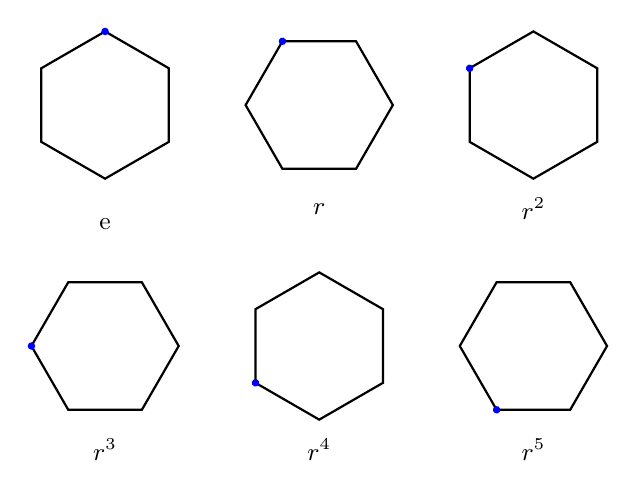
\begin{tikzpicture}[scale=0.85, every node/.style={font=\small}]
  \def\R{1.1}
  \def\Px{0.35}
  \def\Py{0.15}

  % 原图
  \begin{scope}[shift={(0,0)}]
    \draw[thick] (90:\R)
      \foreach \a in {150,210,270,330,30} { -- (\a:\R) } -- cycle;
    \fill[blue] (90:\R) circle (1.6pt);
    \node[below] at (0,-1.55) {e};
  \end{scope}

  % 旋转 30
  \begin{scope}[shift={(3.2,0)}, rotate=30]
    \draw[thick] (90:\R)
      \foreach \a in {150,210,270,330,30} { -- (\a:\R) } -- cycle;
    \fill[blue] (90:\R) circle (1.6pt);
  \end{scope}
  \node at (3.2,-1.55) {$r$};

  % 旋转 60
  \begin{scope}[shift={(6.4,0)}, rotate=60]
    \draw[thick] (90:\R)
      \foreach \a in {150,210,270,330,30} { -- (\a:\R) } -- cycle;
    \fill[blue] (90:\R) circle (1.6pt);
  \end{scope}
  \node at (6.4,-1.55) {$r^2$};

  % 旋转 90
  \begin{scope}[shift={(0,-3.6)}, rotate=90]
    \draw[thick] (90:\R)
      \foreach \a in {150,210,270,330,30} { -- (\a:\R) } -- cycle;
    \fill[blue] (90:\R) circle (1.6pt);
  \end{scope}
  \node at (0,-5.15) {$r^3$};

  % 旋转 120
  \begin{scope}[shift={(3.2,-3.6)}, rotate=120]
    \draw[thick] (90:\R)
      \foreach \a in {150,210,270,330,30} { -- (\a:\R) } -- cycle;
    \fill[blue] (90:\R) circle (1.6pt);
  \end{scope}
  \node at (3.2,-5.15) {$r^4$};

  % 旋转 150
  \begin{scope}[shift={(6.4,-3.6)}, rotate=150]
    \draw[thick] (90:\R)
      \foreach \a in {150,210,270,330,30} { -- (\a:\R) } -- cycle;
    \fill[blue] (90:\R) circle (1.6pt);
  \end{scope}
  \node at (6.4,-5.15) {$r^5$};
\end{tikzpicture}
\end{center}

现在我们来检查一下这个群是否符合公理：

\begin{enumerate}
  \item \textbf{封闭性（Closure）}：将两个不同次数的旋转叠加，输出的结果还是旋转后的某个操作

  \item \textbf{结合律（Associativity）}：旋转$n$次和旋转$m$次的加和是旋转$m+n$次

  从这里我们不难推断$r^5 + r = e$

  \item \textbf{单位元存在（Identity）}：对单位元旋转任意次都可以得到对应次数的图像

  \item \textbf{逆元存在（Inverse）}：逆旋转就好了
\end{enumerate}

显然这个二面体旋转群是一个成立的群

那你也许会很不理解：明明说是讲群论，讲这个二面体群有什么用呢？

事实上，在许多物理问题中，我们都不可能直接通过解方程得到答案，而是认识到它现实中的物理结构是一个

\newpage
\section{群的映射}

三种最常见的映射类型：

\subsection{HOMO / 同态}

考虑两个数字之和，要判断其结果是偶数还是奇数，相信你不会费心计算出结果，而只是判断末尾的情况

同态正是这样的一种操作，它将运算分为奇和偶，在群论中我们不说奇偶，而是将其转化为：

\[
\scalebox{1.3}{$
\begin{array}{c|cc}
+ & \text{even} & \text{odd} \\
\hline
\text{even} & \text{even} & \text{odd} \\
\text{odd} & \text{odd} & \text{even}
\end{array}
$}
\longrightarrow 
\scalebox{1.3}{$
\begin{array}{c|cc}
Z_2 & \text{1} & \text{0} \\
\hline
\text{1} & \text{1} & \text{0} \\
\text{0} & \text{0} & \text{1}
\end{array}
$}
\]

对于其它群也可以有相同的操作，我们称之为同态，一般记为：
\[
G_1 \xrightarrow{\quad \psi \quad } G_2
\]

他表示将$G_1$中的元素转化为$G_2$中更简便的形式，并且保持运算不变，例如：
\[
  1+2=3\xrightarrow{\quad \psi \quad } 2^1\times 2^2=2^3
\]

在这种定义下，无论是最常见的“$\times 7 $”还是“$det $”都是某些层次上的同态映射
\[
A \cdot B = C \xrightarrow{\quad \psi \quad } det(A) \cdot det(B) = det(C)
\]

我们不难发现，同态必须满足一致性原则，这一点很强
\[
a \cdot b = c \xrightarrow{\quad \psi \quad } \psi(a) \cdot \psi(b) = \psi(c)
\]

既然运算的关系一定是满足的，那么对于\textbf{循环群}而言我们不难在只确定一个元素的映射的情况下逆向推导出整个映射，现在让我们考虑一个$Z_8 \xrightarrow{\quad \psi \quad } Z_4$的映射，我们认为$1\xrightarrow{\quad \psi \quad }\psi(1)=1$,那么不难得到
\[
4\xrightarrow{\quad \psi \quad }\psi(1)+\psi(1)+\psi(1)+\psi(1)=1+1+1+1=0
\]

以此类推，我们不难逆向出整个映射：

\[
\begin{tikzcd}[column sep=2.2em, row sep=4.5em]
\mathbb{Z}_8:
& 0 \arrow[drr, mapsto]
& 1 \arrow[drr, mapsto]
& 2 \arrow[drr, mapsto]
& 3 \arrow[drr, mapsto]
& 4 \arrow[dll, mapsto]
& 5 \arrow[dll, mapsto]
& 6 \arrow[dll, mapsto]
& 7 \arrow[dll, mapsto] \\
\mathbb{Z}_4:
&
&
& 0
& 1
& 2
& 3
\end{tikzcd}
\]

你还记得我们第一章节讨论的二面体群吗

旋转和反转，两个看似毫不相关的操作，却可以在同态映射下呈现出显著的奇偶性：

\[
\begin{matrix}
r \cdot r = r^2\\
s \cdot r = sr\\
sr \cdot sr =e
\end{matrix}  
\xrightarrow{\quad \psi \quad }
\begin{matrix}
0 + 0 = 0\\
1 + 0 = 1\\
1 + 1 = 0
\end{matrix}  
\]



这可以极大的简化运算！比方说你要计算$sr \cdot r \cdot sr$，正常计算不难得到其结果为$e$,你可能会画图，或者利用大脑进行一系列空间想象，但是如果存在一个从二面体群到“元素是否翻转”的群，那么我们便可以快速的判断操作的结果：
\[
\psi(sr \cdot r \cdot sr) =s \cdot e \cdot s = e
\]
所以结果就是旋转三次

或者你也可以定义一个“元素是否旋转”的群，它只保留旋转的部分：
\[
\psi(sr \cdot sr ) =r \cdot r = r^2
\]
但是这就出现了错误！这个同态违反了一致性原则，所以这个同态不成立

事实上，不存在同态能将操作简化到只保留旋转，这一点我们可以证明，现在考虑一般群的一个运算，不难写出同态：
\[
\begin{aligned}
a \cdot e &= a \xrightarrow{\quad \psi \quad } \psi(a) \cdot \psi(e)=\psi(a),\\
a \cdot a^{-1} &= e \xrightarrow{\quad \psi \quad } \psi(a) \cdot \psi(a^{-1})=\psi(e).
\end{aligned}
\]

从单位元的定义出发，我们不难意识到任意情况下都满足$\psi(e)=e$,而且变换$\psi$不影响逆元的运算

现在我们再重新考虑二面体群到旋转群的映射，根据上面的信息我们不难得到：

\[
\begin{tikzcd}[column sep=1em, row sep=4.5em]
\mathbb{D}_6:
& e \arrow[drrr, mapsto]
& r 
& r^2 
& r^3 
& r^4 
& r^5
& s 
& sr 
& sr^2 
& sr^3 
& sr^4 
& sr^5 
\\
\mathbb{Z}_6:
&
&
&
& e 
& r 
& r^2 
& r^3 
& r^4 
& r^5 
\end{tikzcd}
\]

但是当我们考虑翻转的时候，问题出现了，翻转的逆元还是自己，但是唯一满足这个条件的只有单位元，这时候带翻转的映射就乱了套了，它只能被映射到单位元
\[
\begin{tikzcd}[column sep=1em, row sep=4.5em]
\mathbb{D}_6:
& e \arrow[drrr, mapsto]
& r \arrow[drr, mapsto]
& r^2 \arrow[dr, mapsto]
& r^3 \arrow[d,mapsto]
& r^4 \arrow[dl, mapsto]
& r^5 \arrow[dll, mapsto]
& s \arrow[dlll, mapsto]
& sr \arrow[dllll, mapsto]
& sr^2 \arrow[dlllll, mapsto]
& sr^3 \arrow[dllllll, mapsto]
& sr^4 \arrow[dlllllll, mapsto]
& sr^5 \arrow[dllllllll, mapsto]
\\
\mathbb{Z}_6:
&
&
&
& e 
& r 
& r^2 
& r^3 
& r^4 
& r^5 
\end{tikzcd}
\]

所以说不存在只保留旋转而筛去翻转的同态，至于为什么，我认为可能是由于翻转是一个于元素相关的操作，取不同的翻转比如斜向翻转，会造成不一样的结果，这说明它不是一个有用的性质


\subsection{ISO / 同构}

我们把正六边形按中心旋转所得到的变换记为
\[
R=\{e,r,r^2,r^3,r^4,r^5\},\qquad r^6=e,
\]
其中 $r$ 表示逆时针旋转 $60^\circ$。在复合运算下，$R$ 构成一个 6 阶循环群。那你难道不觉得$Z_5$正整数群和$D_5$旋转群难道是相同的吗？除了我们书写方式的不同，它们其它的所有运算性质都是相同的，比如说$1+2=3$和$r^1+r^2=r^3$这两种运算除去使用符号不一样，但是表示的意义，在循环中的位置都是一样的！这时候我们说在二者之间存在一个所谓的同构映射，这就是说如果我们定义映射
\[
\varphi:R\to \mathbb{Z}_6,\qquad \varphi(r^k)=\bar{k}\;(k=0,1,\dots,5).
\]
\[
\begin{tikzcd}[column sep=1em, row sep=4.5em]
\mathbb{D}_6:
& e \arrow[d,mapsto]
& r \arrow[d,mapsto]
& r^2 \arrow[d,mapsto]
& r^3 \arrow[d,mapsto]
& r^4 \arrow[d,mapsto]
& r^5\arrow[d,mapsto]
\\
\mathbb{Z}_6:
& e 
& r 
& r^2 
& r^3 
& r^4 
& r^5 
\end{tikzcd}
\]
则对任意 $i,j$，有
\[
\varphi(r^i\circ r^j)=\varphi(r^{i+j})=\overline{i+j}=\bar{i}+\bar{j}
=\varphi(r^i)+\varphi(r^j),
\]
因此 $\varphi$ 其实也是一种是群同态，但是它每一个输出又对应唯一一个输入，而且它是双向的的——每一个同构都存在对应的逆同构。一般而言我们把同构记作：
\[
R\cong \mathbb{Z}_6.
\]

同构是一个十分有用的性质，它允许我们了解我们联系各有优劣的群，有的群很容易理解但不强大；有的群很强大但是你很难理解。而我们只需要证明他同构那么我们就可以把在一侧无法解决的问题通过同构转移到另一侧，在那里计算并用逆同构转移回来来得到结果。
\[
Gal(Q(\xi_5)/Q)\cong\mathbb{Z}_4
\]
为了清楚的理解这个事情，接下来我们来了解一个新的群———乘法群。我们熟悉循环群，例如在$Z_9$中我们可以做加法，比如$5+6=2$，我们可以对乘法做同样的事情，在这个群里$5 \times 6 = 3$，但是有一个问题：乘法并不在这里构成一个群，它不满足每个数都有逆元，特别是$0$，那你也许会想：“那只要删掉没逆元的数字不就好了？”但是这样可能会破坏封闭定理，万一某个乘法结果恰好被我们删掉了呢？
\[
\{0,1,2,3,4,5,6,7,8\}\longrightarrow\{1,2,4,5,7,8\}
\]

在学习线性代数时候我们知道矩阵乘法$a \cdot b $的逆元是 $b^{-1} \cdot a^{-1}$（如果存在的话），这也适用于所有群，这个事实有时被称为袜鞋原则，意思是如果你先穿袜子再穿鞋，那么你反过来一定是先脱鞋再脱袜子。但是这个比喻在这里不是很合适，毕竟对于乘法而言，先穿鞋还是先穿袜子是等价的。总而言之我们要说的是对于剩下的元素，它们的乘法结果一定存在逆元，因为任意存在逆元的$a,b$所构成的新元$a \cdot b $都一定有其逆元$b^{-1} \cdot a^{-1}$，这也就是说我们不可能生成一个没逆元的新元素，所以封闭性其实是满足的。所以它确实是一个群——$\mathbb{Z}_9^{\times}$，这就是$\mathbb{Z}_9$乘法群。

显然这个规律对于任何循环群都是适用的：
\begin{figure}[H]
    \centering
    \begin{tikzpicture}
        % 字号调整
        \tikzset{
            dimstyle/.style={text=dim, font=\large\sffamily}, 
            highlightstyle/.style={text=highlight, font=\large\sffamily},
            labelstyle/.style={text=labelcolor, font=\Large\sffamily\bfseries}
        }

        % 定义 X 和 Y 坐标偏移量
        \def\xoff{2.2}
        \def\ybase{0}

        % ---- 第一行: Z6^x ----
        \node[labelstyle, anchor=east] at (\xoff-0.5, 0) {\(Z_6^\times\)};
        \node[dimstyle] at (\xoff+0, 0) {0};
        \node[highlightstyle] at (\xoff+1.0, 0) {1};
        \node[dimstyle] at (\xoff+2.0, 0) {2};
        \node[dimstyle] at (\xoff+3.0, 0) {3};
        \node[dimstyle] at (\xoff+4.0, 0) {4};
        \node[highlightstyle] at (\xoff+5.0, 0) {5};

        % ---- 第二行: Z7^x ----
        \node[labelstyle, anchor=east] at (\xoff-0.5, -1.2) {\(Z_7^\times\)};
        \node[dimstyle] at (\xoff+0, -1.2) {0};
        \node[highlightstyle] at (\xoff+1.0, -1.2) {1};
        \node[highlightstyle] at (\xoff+2.0, -1.2) {2};
        \node[highlightstyle] at (\xoff+3.0, -1.2) {3};
        \node[highlightstyle] at (\xoff+4.0, -1.2) {4};
        \node[highlightstyle] at (\xoff+5.0, -1.2) {5};
        \node[highlightstyle] at (\xoff+6.0, -1.2) {6};

        % ---- 第三行: Z8^x ----
        \node[labelstyle, anchor=east] at (\xoff-0.5, -2.4) {\(Z_8^\times\)};
        \node[dimstyle] at (\xoff+0, -2.4) {0};
        \node[highlightstyle] at (\xoff+1.0, -2.4) {1};
        \node[dimstyle] at (\xoff+2.0, -2.4) {2};
        \node[highlightstyle] at (\xoff+3.0, -2.4) {3};
        \node[dimstyle] at (\xoff+4.0, -2.4) {4};
        \node[highlightstyle] at (\xoff+5.0, -2.4) {5};
        \node[dimstyle] at (\xoff+6.0, -2.4) {6};
        \node[highlightstyle] at (\xoff+7.0, -2.4) {7};

        % ---- 第四行: Z9^x (无框) ----
        \node[labelstyle, anchor=east] at (\xoff-0.5, -3.6) {\(Z_9^\times\)};
        \node[dimstyle] at (\xoff+0, -3.6) {0};
        \node[highlightstyle] at (\xoff+1.0, -3.6) {1};
        \node[highlightstyle] at (\xoff+2.0, -3.6) {2};
        \node[dimstyle] at (\xoff+3.0, -3.6) {3};
        \node[highlightstyle] at (\xoff+4.0, -3.6) {4}; % 这里的4保留显色
        \node[highlightstyle] at (\xoff+5.0, -3.6) {5};
        \node[dimstyle] at (\xoff+6.0, -3.6) {6};
        \node[highlightstyle] at (\xoff+7.0, -3.6) {7};
        \node[highlightstyle] at (\xoff+8.0, -3.6) {8};

        % ---- 第五行: Z10^x ----
        \node[labelstyle, anchor=east] at (\xoff-0.5, -4.8) {\(Z_{10}^\times\)};
        \node[dimstyle] at (\xoff+0, -4.8) {0};
        \node[highlightstyle] at (\xoff+1.0, -4.8) {1};
        \node[dimstyle] at (\xoff+2.0, -4.8) {2};
        \node[highlightstyle] at (\xoff+3.0, -4.8) {3};
        \node[dimstyle] at (\xoff+4.0, -4.8) {4};
        \node[dimstyle] at (\xoff+5.0, -4.8) {5};
        \node[dimstyle] at (\xoff+6.0, -4.8) {6};
        \node[highlightstyle] at (\xoff+7.0, -4.8) {7};
        \node[dimstyle] at (\xoff+8.0, -4.8) {8};
        \node[highlightstyle] at (\xoff+9.0, -4.8) {9};

    \end{tikzpicture}
\end{figure}
我们观察这些被剔除的数字，不难发现这些数字基本都和循环群元素总个数存在公因数，这也解释了为什么$\mathbb{Z}_7$这样的质数循环群基本保留了所有的元素。如果你懂数论那么你一定可以证明这个事情一定成立，可惜这里我们要说的是群论，所以我就不在这里证明了毕竟地方太小写不下。

这是一个十分有趣的性质，也正是乘法群这个公因数的性质使得质数循环群$\mathbb{Z}_p$格外受到计算机科学家的青睐，尤其是在Difffie-Hellman密钥交换和RSA加密系统都利用它来进行安全的信息交换。

这里我们先来了解一个新概念——平方剩余，指$\mathbb{Z}_p^{\times}$中的平方数，它有一个十分有趣的性质，就是这个群中恰好有一半的数字都可以表示为平方数，比如$\mathbb{Z}_{11}^{\times}$中$4\times4=5$，同样的1，3，4，5，9都是平方剩余。在我们的认知中随着数字增大，平方数会越来越系数，但是在$\mathbb{Z}_p^{\times}$中不是，总是有一半的数字是平方剩余。这个性质被用来制作公平的随机数，比如两个电脑一起抛硬币，电脑完全可以发送更有利于自己的结果，那么这时候就可以利用$\mathbb{Z}_p^{\times}$的性质，将两个电脑发送的结果在$\mathbb{Z}_p^{\times}$上运算，即使一方发送了非随机的数字，在运算后也可以坍缩为完全的随机数。为什么呢？这里有一个有趣的性质，就是：
\[
\mathbb{Z}_p^{\times} \cong \mathbb{Z}_{p-1}
\]
这看起来十分的不可思议，毕竟一个是乘法群，一个是加法群。很不幸的是，这种同构完全没有任何规律，不过它确实是存在的。
\[
\begin{tikzcd}[column sep=1em, row sep=4.5em]
\mathbb{Z}_{11}^{\times}:
& 1 \arrow[d,mapsto]
& 2 \arrow[d,mapsto]
& 3 \arrow[drrrrrr,mapsto]
& 4 \arrow[dl,mapsto]
& 5 \arrow[d,mapsto]
& 6 \arrow[drrrr,mapsto]
& 7 \arrow[dr,mapsto]
& 8 \arrow[dllll,mapsto]
& 9 \arrow[dll,mapsto]
& 10 \arrow[dllll,mapsto]
\\
\mathbb{Z}_{10}:
& 0 
& 1 
& 2
& 3 
& 4 
& 5
& 6
& 7
& 8
& 9
\end{tikzcd}
\]
这时候平方的运算在$\mathbb{Z}_{10}$中就会转化为一个数加上它自己，而这样加和的结果总是偶数。观察上图你也不难发现所有的平方数最终都被映射为$\mathbb{Z}_{10}$中的偶数，而$\mathbb{Z}_{10}$中有一半是偶数，因此$\mathbb{Z}_{11}^{\times}$中也有一半是平方数。


\subsection{AUTO / 自同构}
同构是群结果相似，显然每个群一定和自己是相似的，所以它叫自同构。我们一定可以写出这样的自同构，这很显然，但问题是我们能写出几种自同构？除去平凡的自同构，我们还可以将所有数字映射为自身的相反数
\[
\begin{tikzcd}[column sep=1em, row sep=4.5em]
\mathbb{Z}:
& -5 \arrow[drrrrrrrrrr,mapsto]
& -4 \arrow[drrrrrrrr,mapsto]
& -3 \arrow[drrrrrr,mapsto]
& -2  \arrow[drrrr,mapsto]
& -1  \arrow[drr,mapsto]
&  0 \arrow[d,mapsto]
&  1 \arrow[dll,mapsto]
&  2 \arrow[dllll,mapsto]
&  3 \arrow[dllllll,mapsto]
&  4 \arrow[dllllllll,mapsto]
&  5 \arrow[dllllllllll,mapsto]
\\
\mathbb{Z}:
& -5
& -4
& -3
& -2 
& -1 
&  0
&  1
&  2 
&  3 
&  4 
&  5 
\end{tikzcd}
\]
一个群可以有多种自同构，比如$\mathbb{Z}_{9}$，它有足足6种自同构，这也十分好验证，只要我们对其中的单位元遍历映射每一个其它元上，我们就可以总结出所有成立的自同构了。如果你演算了这个过程，那么你会发现将$1$映射到${1,2,4,5,7,8}$中的元素的时候构成自同构，这并非独有现象，如果你对其它循环群做同样的测试，你会发现它们的自同构群也会很像对应的乘法群，那么问题来了，为什么呢？

首先自同构和同态不一样，同态会把原来的群变成新的东西，我要么找逆同态变回去，要么找新的同态转化，但是自同构不一样，你可以任意的建立任意次映射，群总还是它自己，它不仅保留了原有的运算系统，还有一整个元系统（各种映射函数），在这个元系统里你可以对这些自同构进行运算，你也不难猜到这些元系统也构成一个群，相信你学了这么多一定可以自己验证了吧！我给个提示，单位元是恒等自同构，也就是恒等映射$Id$，而组合恒等同构和任意其它同构，得到的效果$Id \cdot \psi = \psi$和$e \cdot a =a$的效果是一样的，所以其实逆同构就有$\psi \cdot \psi^{-1} = Id$，这正是逆元的行为！总而言之一个群所有的自同构映射函数就被成为自同构群，它被记为$Aut(G)$。

正如你所想，揭示并分析任意群的自同构群是群论的一个重要课题，但在我们这里我们专注于$Aut(Z_9)$，那么我们之前看到的规律就可以被描述为：
\[
Aut(Z_9) \cong \mathbb{Z}_{9}^{\times}
\]
我们先来看看把$1$映射为$2$的自同构，也就是$1+2=3$会变成$2+4=6$，作为物理学家，我们可以直观的说这个操作就是把整个式子乘了$2$倍，而$2$没有特别之处，任何这样的操作都其实只是乘以$n$的倍数，当然必要下会在$mod9$下循环回来，这已经暗示了和$\mathbb{Z}_{9}^{\times}$的联系。我们知道自同构可以被任意组合，也就是我们先乘$2$然后再乘$5$，这等价于直接乘$10$，但是再$\mathbb{Z}_{9}$的语境下这就不成立了，你无法把$1$映射到$10$，它本就不存在于这个群中，所以它其实的运算效果最后就是$\times 1$，这我们在$\mathbb{Z}_{9}^{\times}$有完全对应的关系，只是表达不是很一样，而这进一步解释了为什么映射到${0,3,6}$的自同构不存在，根据定义自同构一定有对应的逆，但是这三个元在$\mathbb{Z}_{9}^{\times}$中本来就没有逆元，怎么会存在自同构？唯一合理的结论就是它根本不存在自同构，这最终证明了我们想要展示的结论。但实际上运用同样的逻辑，我们也可以证明：
\[
Aut(Z_n) \cong \mathbb{Z}_{n}^{\times}
\]
这是自同构理论中最基本的知识。

让我们来看一个更复杂的自同构群，也就是最初提到的二面体群：
\[
\begin{tikzcd}[column sep=1em, row sep=4.5em]
\mathbb{D}_5:
& e \arrow[drrr, mapsto]
& r 
& r^2 
& r^3 
& r^4 
& s 
& sr 
& sr^2 
& sr^3 
& sr^4 
\\
\mathbb{Z}_5:
& e 
& r 
& r^2 
& r^3 
& r^4 
& s 
& sr 
& sr^2 
& sr^3 
& sr^4 
\end{tikzcd}
\]
以$D_5$为例我们来找出它所有可能的自同构，我们从单位旋转来逆向推导，结果发现它不能被映射到任何翻转上，因为它具有性质连续两次反转便会回到单位元。所以我们暂时忽略翻转，这时候它就退化为一个$Z_5$群，对我们而言，$Aut(Z_5) \cong \mathbb{Z}_{5}^{\times}$，所以：
\[
\begin{tikzcd}[column sep=1em, row sep=4.5em]
\mathbb{Z}_5:
& e 
& r \arrow[d, mapsto] \arrow[dr, mapsto]\arrow[drr, mapsto]\arrow[drrr, mapsto]
& r^2 
& r^3 
& r^4 
\\
\mathbb{Z}_5:
& e 
& r 
& r^2 
& r^3 
& r^4 
\end{tikzcd}
\]
至此我们已经完成了一半，回到二面体群，我们有：
\[
\begin{tikzcd}[column sep=1em, row sep=4.5em]
\mathbb{D}_5:
& e 
& r \arrow[d, mapsto] \arrow[dr, mapsto]\arrow[drr, mapsto]\arrow[drrr, mapsto]
& r^2 
& r^3 
& r^4 
& s 
& sr 
& sr^2 
& sr^3 
& sr^4 
\\
\mathbb{Z}_5:
& e 
& r 
& r^2 
& r^3 
& r^4 
& s 
& sr 
& sr^2 
& sr^3 
& sr^4 
\end{tikzcd}
\]
无论我们对旋转选择哪个自同构，它们都只忙于在旋转间映射，所以翻转就不可能再映射到某个旋转上了，可能的候选只剩下其它的翻转操作。显然任何翻转都是可以的，附带旋转的翻转其实就是略微倾斜的翻转，所以其实它的自同构就像
\[
\begin{tikzcd}[column sep=1em, row sep=4.5em]
\mathbb{D}_5:
& e 
& r \arrow[d, mapsto] \arrow[dr, mapsto]\arrow[drr, mapsto]\arrow[drrr, mapsto]
& r^2 
& r^3 
& r^4 
& s \arrow[d, mapsto] \arrow[dr, mapsto]\arrow[drr, mapsto]\arrow[drrr, mapsto]\arrow[drrrr, mapsto]
& sr 
& sr^2 
& sr^3 
& sr^4 
\\
\mathbb{Z}_5:
& e 
& r 
& r^2 
& r^3 
& r^4 
& s 
& sr 
& sr^2 
& sr^3 
& sr^4 
\end{tikzcd}
\]
这样我们就找到了所有的自同构，是不是比解析原来的群更简单？

\chapter{概率论}

和群论一样，概率论也是从一片看似完全不同的土壤里长出来的——它的根扎在赌徒的骰子和保险商的账本里，却在十九世纪末被统计物理学家一把拽进了自然法则的核心。今天回头看，这件事近乎奇迹：描述人类无知的工具，恰好也是描述自然最深层结构的语言。

经典力学给世界画出的是一幅确定性的图景：给定初始位置和动量，哈密顿方程告诉你系统过去和未来的全部历史。拉普拉斯那个著名的“妖”就站在这里——只要知道宇宙中每个粒子的当前位置和速度，它就能算出整个未来。这幅图景在逻辑上无懈可击，在实践中却毫无用处。一摩尔气体包含 $N_A\approx 6.022\times 10^{23}$ 个分子，写下它们的全部运动方程不但是不可能的，也是没有意义的——我们并不关心每个分子在哪里，我们关心的是压强、温度、熵这些少数几个宏观量。

正是这种“主观的无知”和“客观的规律”之间的张力，催生了统计物理学，也重新定义了概率论的角色。从麦克斯韦和玻尔兹曼开始，宏观热力学量不再被视为严格确定的值，而是微观状态的概率加权平均。一个孤立的平衡系统，其微观状态在等能量面上均匀分布——这是统计物理学的第一块基石，称为微正则系综。状态数 $\Omega(E)$ 的对数定义了熵：
\[
S=k_B\ln\Omega(E),
\]
其中 $k_B$ 是玻尔兹曼常数。这个公式刻在玻尔兹曼的墓碑上，它把热力学第二定律从一个能量“总是流向下坡”的朴素经验陈述，重新解释为一个严格的概率命题：系统向平衡态演化，不过是从概率极小的宏观状态走向概率极大的宏观状态。熵增不是自然的强迫，而是统计学上的压倒性优势。把一杯热水放在冷房间里之后，热量从热水流向冷水的概率比反过来大得太多了——多到违反它的可能性在我们这个宇宙的寿命尺度上从来没有发生过。

当系统和外界有热接触而交换能量时，微正则系综让位给正则系综。一个处于温度 $T$ 的平衡系统，其微观状态 $i$ 出现的概率由玻尔兹曼分布给出：
\[
P_i=\frac{1}{Z}e^{-E_i/k_BT},\qquad Z=\sum_i e^{-E_i/k_BT}.
\]
这里 $Z$ 是配分函数，它不只是一个归一化常数，而是通往所有热力学量的钥匙。亥姆霍兹自由能 $F=-k_BT\ln Z$，内能 $U=-\partial\ln Z/\partial\beta$，熵 $S=k_B(\ln Z+\beta U)$——整个热力学从配分函数中流水般地涌出。概率在这里不再是认知缺陷的标记，而成了物理预言的有机构成部分。你不必跟踪 $10^{23}$ 个粒子的轨迹，你只需要计算配分函数，它打包了全部统计信息的精华。

吉布斯把这个框架推到了极致。他引入的三套系综——微正则、正则、巨正则——每一套对应一组不同的物理约束，却都建立在一个共同的概率假设上：在给定的宏观约束下，所有与之相容的微观状态等可能。这个假设被称为等概率原理，它没有更基本的证明，但它的推论和实验吻合得如此彻底，以至于任何怀疑它的人都必须同时怀疑整个统计物理学大厦的可靠程度。巨正则系综允许系统和外界交换粒子，其配分函数推广为巨配分函数：
\[
\Xi=\sum_{N=0}^{\infty}e^{\beta\mu N}Z_N,
\]
其中 $\mu$ 是化学势。这个推广使得我们可以处理相变、量子气体的玻色-爱因斯坦凝聚、费米气体的低温行为——所有这些现象，最终都归结为概率分布的形式和一个求和。

从统计物理学的视角看，概率论的本质变得异常清晰：它不是我们对世界“知道得还不够多”时用的权宜之计，而是处理复杂系统时把微观信息“粗粒化”的系统方法。即使底层动力学是完全确定性的（量子力学另当别论），只要系统的自由度足够多，宏观行为就会以压倒性的概率锁定在热力学的预言上。大数定律和中心极限定理是这个过程的数学心脏：大量独立随机变量的和在极限下趋向正态分布——而一个含 $10^{23}$ 个粒子的系统，其物理量的涨落通常按 $1/\sqrt{N}$ 衰减，相对涨落小到观测不到。这就是为什么确定性方程能描述宏观世界：不是因为自然没有随机性，而是因为随机性的聚集效应把涨落压到了可忽略的数量级。

玻尔兹曼、麦克斯韦和吉布斯为概率论授予了一张自然科学的入场券。从此以后，概率不再是赌徒掷骰子时对下一面的猜测，而是温度、压强、相变的本质。它同时承诺了两件事：一方面，单个粒子的运动不值得追踪；另一方面，大量粒子的集体行为精确到令人尊敬。统计物理学矗立在这两种直觉的交界处，而概率是它唯一需要的通用语言。

\newpage
\section{概率论基本知识}
\subsection{概率空间}
定义概率空间 $(\Omega,\mathcal{F},P)$：$\Omega$ 为样本空间，$\mathcal{F}$ 为事件域，$P$ 为测度。

集合上极限：
\[
\lim_{n\to\infty}\sup A_n=\bigcap_{k=1}^{\infty}\bigcup_{n=k}^{\infty}A_n,
\]
下极限：
\[
\lim_{n\to\infty}\inf A_n=\bigcup_{k=1}^{\infty}\bigcap_{n=k}^{\infty}A_n.
\]

\subsection{随机变量}
随机变量 $X:(\Omega,\mathcal{F})\to(\mathbb{R},\mathcal{B}(\mathbb{R}))$。分布函数
\[
F(x)=P\{\omega:X(\omega)<x\},
\]
概率测度 $\mu((a,b])=F(b)-F(a)$，诱导 $\sigma$-代数 $\sigma(X)=X^{-1}(B)$。

\paragraph{四种收敛模式}
\begin{itemize}
  \item 几乎必然收敛：$P\{\omega:\lim_{n\to\infty}X_n(\omega)=X(\omega)\}=1$，记 $X_n\to X$ (a.s.)。
  \item 依概率收敛：$\forall\varepsilon>0,\ \lim_{n\to\infty}P(|X_n-X|\ge\varepsilon)=0$，记 $X_n\to X$ (P)。
  \item 依分布收敛：对 $F$ 的每个连续点 $x$，$\lim_{n\to\infty}F_n(x)=F(x)$，记 $X_n\to X$ (d)。
  \item $r$ 阶矩收敛：$r>0,\ \lim_{n\to\infty}\mathbb{E}(|X_n-X|^r)=0$，记 $X_n\to X$ in $L^r$。
\end{itemize}

\begin{figure}[htbp]
  \centering
  \begin{tikzpicture}[
    box/.style={draw,rounded corners=2pt,inner sep=3pt,minimum height=8mm,align=center},
    arrow/.style={-{Stealth[length=2mm]},semithick},
    node distance=8mm and 14mm
  ]
    \node[box,fill=cyan!10] (as) {几乎必然收敛};
    \node[box,fill=cyan!10,below=of as] (lr) {$r$ 阶矩收敛};
    \node[box,fill=green!10,right=16mm of $(as)!0.5!(lr)$] (p) {依概率收敛};
    \node[box,fill=gray!10,right=14mm of p] (d) {依分布收敛};

    \draw[arrow] (as) -- (p);
    \draw[arrow] (lr) -- (p);
    \draw[arrow] (p) -- (d);
  \end{tikzpicture}
  \caption{随机变量的几种收敛关系示意图}
\end{figure}



\section{概率学的几种定理}
\subsection{大数定律}
大数定律描述：当试验次数足够多时，随机事件的平均值会稳定地趋近于理论期望值。

\subsubsection{切比雪夫弱大数定律}
切比雪夫不等式：若 $\mathbb{E}X=\mu$，$\mathrm{Var}(X)=\sigma^2$，则对任意 $\varepsilon>0$，
\[
P\{|X-\mu|\ge \varepsilon\}\le \frac{\sigma^2}{\varepsilon^2}.
\]
弱大数定律（示意）：
\[
\frac{1}{n}\sum_{k=1}^n X_k \xrightarrow{P} \frac{1}{n}\sum_{k=1}^n \mu_k,\qquad (n\to\infty).
\]

\subsection{中心极限定律}
无论单个随机变量原本是什么分布，只要数量足够多，它们的和的分布就“看起来像”正态分布。

\subsection{特征函数}
\[
\varphi_X(t)=\mathbb{E}\bigl[e^{itX}\bigr].
\]
连续型随机变量可写为
\[
\varphi_X(t)=\int_{-\infty}^{\infty} e^{itx}f(x)\,dx.
\]
可把指数展开为级数再取期望：
\[
\varphi_X(t)=\mathbb{E}\!\left[1+\frac{itX}{1!}+\frac{(itX)^2}{2!}+\frac{(itX)^3}{3!}+\cdots\right].
\]

因为 $\mathbb{E}$ 是线性的，所以
\[
\varphi_X(t)
=\mathbb{E}[1]+it\,\mathbb{E}[X]+\frac{(it)^2}{2!}\mathbb{E}[X^2]+\frac{(it)^3}{3!}\mathbb{E}[X^3]+\cdots.
\]
由此可通过特征函数求矩（矩生成关系）：
\[
\mathbb{E}[X^k]=\frac{\varphi_X^{(k)}(0)}{i^k}.
\]
特别地，
\[
\mathbb{E}[X]=-i\varphi_X'(0),
\qquad
\mathrm{Var}(X)=\mathbb{E}\!\bigl[(X-\mathbb{E}[X])^2\bigr]
=-\varphi_X''(0)+\bigl(\varphi_X'(0)\bigr)^2.
\]

\section{概率模型}
\subsection{泊松过程}
设 $\{N(t),t\ge 0\}$ 表示时间区间 $[0,t]$ 上事件发生次数，满足 $N(0)=0$。对 $0\le t_1<t_2<\cdots<t_n$，考虑增量
\[
N(t_2)-N(t_1),\ N(t_3)-N(t_2),\ \dots,\ N(t_n)-N(t_{n-1}),
\]
也可写作 $N(t+s)-N(s)$。若 $N(t+s)-N(s)$ 的分布与 $s$ 无关（只与时间间隔 $t$ 有关），则
\[
P(N(t)=k)=\frac{(\lambda t)^k e^{-\lambda t}}{k!},\qquad k=0,1,2,\dots
\]
其期望与方差为
\[
\mathbb{E}[N(t)]=\lambda t,\qquad \mathrm{Var}[N(t)]=\lambda t.
\]

\subsubsection{复合泊松过程}
设
\[
X(t)=\sum_{i=1}^{N(t)}Y_i,
\]
其中 $Y_i$ 为独立同分布随机变量序列，可描述随时间的累加效应。其期望与方差：
\[
\mathbb{E}[X(t)]=\lambda t\,\mathbb{E}[Y],\qquad \mathrm{Var}[X(t)]=\lambda t\,\mathbb{E}[Y^2].
\]
简要推导：
\[
\mathbb{E}[X(t)]=\mathbb{E}\bigl[\mathbb{E}[X(t)\mid N(t)]\bigr]
=\mathbb{E}[N(t)\mathbb{E}[Y]]
=\mathbb{E}[Y]\mathbb{E}[N(t)]
=\lambda t\,\mathbb{E}[Y],
\]
\[
\mathrm{Var}[X(t)]
=\mathbb{E}\bigl[\mathrm{Var}[X(t)\mid N(t)]\bigr]
\mathrm{Var}\bigl[\mathbb{E}[X(t)\mid N(t)]\bigr]
=\lambda t\,\mathrm{Var}[Y]+\lambda t(\mathbb{E}[Y])^2
=\lambda t\,\mathbb{E}[Y^2].
\]

\subsubsection{条件泊松过程}
概率函数
\[
P(N(t)=k)=\mathbb{E}\!\left[\frac{(\Lambda t)^k e^{-\Lambda t}}{k!}\right],
\]
其中 $\Lambda$ 为随机变量，适用于个体差异导致“方差远大于均值”的计数数据。其期望与方差为
\[
\mathbb{E}[N(t)]=t\,\mathbb{E}[\Lambda],\qquad
\mathrm{Var}[N(t)]=t\,\mathbb{E}[\Lambda]+t^2\mathrm{Var}[\Lambda].
\]

\subsubsection{非齐次泊松过程}
在非齐次泊松过程中 $\lambda$ 为时间函数 $\lambda(t)$。定义均值函数
\[
m(t)=\int_0^t \lambda(u)\,du,
\]
则
\[
P(N(t)=k)=\frac{m(t)^k e^{-m(t)}}{k!},\qquad k=0,1,2,\dots
\]
且
\[
\mathbb{E}[N(t)]=m(t),\qquad \mathrm{Var}[N(t)]=m(t).
\]






\end{document}
